%% ----------------------------------------
%%
%% NYU PhD thesis template.
%% Created by José Koiller 2007--2008.
%% Modified by Siddharth Krishna, 2019.
%% Template available at https://github.com/siddharth-krishna/nyu-thesis-template
%%
%% ----------------------------------------


%% Use the first of the following lines during production to
%% easily spot "overfull boxes" in the output. Use the second
%% line for the final version.
%\documentclass[12pt,draft,letterpaper]{report}
\documentclass[12pt,oneside,letterpaper]{report}


% ----------------------------------------
% Macro to switch between draft version and final version
% ----------------------------------------

% Use or comment this to enable/disable draft version
% \def\draftversion{}
\newcommand{\draftfinal}[2]{\ifdefined\draftversion#1\else#2\fi}
\newcommand{\draftonly}[1]{\draftfinal{#1}{}}
\newcommand{\finalonly}[1]{\draftfinal{}{#1}}


% ----------------------------------------
% Thesis metadata
% ----------------------------------------

%% Replace the title, name, advisor name, graduation date and dedication below
%% with your own. Graduation months must be January, May or September.
\newcommand{\thesistitle}{Techniques for Sample-Efficient Reinforcement Learning}
\newcommand{\thesisauthor}{William Fairclough Whitney}
\newcommand{\thesisadvisor}{Professor Kyunghyun Cho}
\newcommand{\thesisdept}{Computer Science}
\newcommand{\gradmonth}{September}
\newcommand{\gradyear}{2021}

%% If you do not want a dedication, scroll down and comment out
%% the appropriate lines in this file.
\newcommand{\thesisdedication}{To my dog Weierstra\ss, with affection.}

% ----------------------------------------
% Layout and formatting
% ----------------------------------------

% Uncomment to get a big black box to spot "overfull hboxes"
% \setlength{\overfullrule}{5pt}



%% Color definitions:
\RequirePackage[prologue]{xcolor}
\definecolor[named]{ThesisBlue}{cmyk}{1,0.1,0,0.1}
\definecolor[named]{ThesisYellow}{cmyk}{0,0.16,1,0}
\definecolor[named]{ThesisOrange}{cmyk}{0,0.42,1,0.01}
\definecolor[named]{ThesisRed}{cmyk}{0,0.90,0.86,0}
\definecolor[named]{ThesisLightBlue}{cmyk}{0.49,0.01,0,0}
\definecolor[named]{ThesisGreen}{cmyk}{0.20,0,1,0.19}
\definecolor[named]{ThesisPurple}{cmyk}{0.55,1,0,0.15}
\definecolor[named]{ThesisDarkBlue}{cmyk}{1,0.58,0,0.21}

% School color found from university's graphic identity site:
% http://www.nyu.edu/employees/resources-and-services/media-and-communications/styleguide.html
\definecolor{SchoolColor}{rgb}{0.3412, 0.0235, 0.5490} % purple
\definecolor{chaptergrey}{rgb}{0.2600, 0.0200, 0.4600} % dialed back a little
\definecolor{midgrey}{rgb}{0.4, 0.4, 0.4}

\usepackage{hyperref}
\hypersetup{colorlinks,
  linkcolor=ThesisDarkBlue,
  citecolor=ThesisPurple,
  urlcolor=ThesisDarkBlue,
  filecolor=ThesisDarkBlue}


%% Captions of Figures, tables
\RequirePackage[labelfont={bf,sf,small,singlespacing},
                textfont={sf,small,singlespacing},
                % justification={justified,RaggedRight},
                % singlelinecheck=false,
                margin=0pt,
                figurewithin=chapter,
                tablewithin=chapter]{caption}

%% Chapter headings, captions
\usepackage{fix-cm}
\RequirePackage[raggedright,sc]{titlesec}
\definecolor{gray75}{gray}{0.75}
\newcommand{\hsp}{\hspace{20pt}}

\titleformat{\chapter}[hang]
{\Huge\sc}
{\textcolor{SchoolColor}{\thechapter}\hsp\textcolor{gray75}{|}\hsp}
{0pt}{\Huge\sc\raggedright}
% [\textcolor{gray75}{|}\hsp\textcolor{SchoolColor}{\thechapter}]


%% The following makes chapters and sections, but not subsections,
%% appear in the TOC (table of contents). Increase to 2 or 3 to
%% make subsections or subsubsections appear, respectively. It seems
%% to be usual to use the "1" setting, however.
\setcounter{tocdepth}{2}

%% Sectional units up to subsubsections are numbered. To number
%% subsections, but not subsubsections, decrease this counter to 2.
\setcounter{secnumdepth}{3}

%% Use the following commands, if desired, during production.
%% Comment them out for final version.
%\usepackage{layout} % defines the \layout command, see below
% TODO: remove this
% \usepackage{geometry}
% \geometry{
  %   right=2in,
  % }
\usepackage[margin=1in, includefoot, letterpaper]{geometry}
\geometry{marginpar=1.6in}
\setlength{\hoffset}{-.75in} % creates a large right margin for notes and \showlabels
%% Page layout (customized to letter paper and NYU requirements):

%% Controls spacing between lines (\doublespacing, \onehalfspacing, etc.):
\usepackage{setspace}

%% Use the line below for official NYU version, which requires
%% double line spacing. For all other uses, this is unnecessary,
%% so the line can be commented out.
\finalonly{
  \doublespacing % requires package setspace, invoked above
}




% ----------------------------------------
% User-specific packages and macros
% ----------------------------------------

%% This inputs your auxiliary file with \usepackage's and \newcommand's:
%% It is assumed that that file is called "defs.tex".
% ----------------------------------------
% Packages
% ----------------------------------------

%
% Place here your \usepackage's. Some recommended packages are already included.
%


\usepackage{lipsum}
% \usepackage{todonotes}
\usepackage{marginnote}
\usepackage{marginfit}
\usepackage{enotez}
\setenotez{
  backref=true,
  }
\usepackage{outlines}



% ----------------------------------------
% Comments and TODOs:
% ----------------------------------------

% Uncomment this to remove all comments
% \newcommand{\nocomments}{}

% Uncomment this to remove all TODOs
% \newcommand{\notodos}{}

% Comments and TODOs
% \newcommand{\fcomment}[2]{\ifdefined\nocomments{}\else\footnote{\textcolor{red}{#1:} #2}\fi}
% % \newcommand{\todo}[1]{\ifdefined\notodos{}\else\textcolor{red}{TODO\ifstrempty{#1}{}{: #1}}\fi}
% \newcommand{\ftodo}[1]{\ifdefined\notodos{}\else\fcomment{TODO}{#1}\fi}

\newcommand{\side}[1]{\ifdefined\nocomments{}\else\marginpar{
  \raggedright \setstretch{1.0} \footnotesize\textcolor{red}{#1} }\fi}

\newcommand{\sideline}[1]{\ifdefined\nocomments{}\else\marginnote{
  \raggedright \setstretch{1.0} \footnotesize\textcolor{red}{#1} }\fi}



% Graphics:
\usepackage[final]{graphicx}
%\usepackage{graphicx} % use this line instead of the above to suppress graphics in draft copies
%\usepackage{graphpap} % \defines the \graphpaper command

% Uncomment this to indent first line of each section:
% \usepackage{indentfirst}

% Good AMS stuff:
\usepackage{amsthm} % facilities for theorem-like environments
\usepackage[tbtags]{amsmath} % a lot of good stuff!

% Fonts and symbols:
\usepackage{amsfonts}
\usepackage{amssymb}

% Set the fonts
\RequirePackage[T1]{fontenc}
\ifxetex
  \RequirePackage[tt=false]{libertine}
\else
  \RequirePackage[tt=false, type1=true]{libertine}
\fi
\RequirePackage[varqu]{zi4}
\RequirePackage[libertine]{newtxmath}


% For typesetting inference rules
\usepackage{mathpartir}
% \usepackage{pftools}  % A local package
\newcommand{\bmmax}{2}
\usepackage{bm}

% Formatting tools:
%\usepackage{relsize} % relative font size selection, provides commands \textsmalle, \textlarger
%\usepackage{xspace} % gentle spacing in macros, such as \newcommand{\acims}{\textsc{acim}s\xspace}

% Page formatting utility:
%\usepackage{geometry}

\usepackage{booktabs}   %% For formal tables:
                        %% http://ctan.org/pkg/booktabs
\usepackage[labelformat=simple]{subcaption} %% For complex figures with subfigures/subcaptions
                        %% http://ctan.org/pkg/subcaption
% Options to subcaption are to label and refer to subfigures as Fig 1(a) etc.
\renewcommand\thesubfigure{(\alph{subfigure})}

\usepackage[T1]{fontenc} % needed for scaling fancy fonts (?)
\usepackage[utf8]{inputenc} % not sure this is needed

\usepackage{amssymb}
%\usepackage[table]{xcolor}

% For code
\usepackage[final]{listings}
\lstset{mathescape=true}

% For code highlighting
% \usepackage{bold-extra}

% Tikz
\usepackage{tikz}
\usetikzlibrary{matrix,arrows,positioning,calc,fit,backgrounds}

% To control enum item labelling/numbering
\usepackage[shortlabels, inline]{enumitem}
% To give custom item labels and reference them
\makeatletter
\newcommand{\myitem}[1][]{
  \protected@edef\@currentlabel{#1}%
\item[#1]
}
\makeatother

% To stop aligned env swallowing up []s
\usepackage{mathtools}

% To use ifstrempty
\usepackage{etoolbox}

% For math mode tables
\usepackage{array}
% A text column in array
\newcolumntype{L}{>$l<$}

% For \llbracket and \rrbracket
\usepackage{stmaryrd}

% For dashed boxes
\usepackage{dashbox}

% For big separating conjunction
\usepackage{scalerel}

% For mathpar environment
\usepackage{mathpartir}

\usepackage{xspace}
\usepackage{multirow}

% To stop citations overflowing lines
\usepackage{breakcites}

% For citet command
\usepackage{natbib}
\setcitestyle{%
    authoryear,%
    open={[},close={]},citesep={;},%
    aysep={},yysep={,},%
    notesep={, }}
\let\cite\citep

%%
%% Place here your \newtheorem's:
%%

\theoremstyle{plain}
\newtheorem{theorem}{Theorem}[chapter]
\newtheorem{conjecture}[theorem]{Conjecture}
\newtheorem{proposition}[theorem]{Proposition}
\newtheorem{lemma}[theorem]{Lemma}
\newtheorem{corollary}[theorem]{Corollary}
\theoremstyle{definition}
\newtheorem{example}[theorem]{Example}
\newtheorem{definition}[theorem]{Definition}
\theoremstyle{plain}


% ----------------------------------------
% Generic definitions
% ----------------------------------------
% Required packages: listings, tikz

% A footnote without a marker
\newcommand\blfootnote[1]{%
  \begingroup
  \renewcommand\thefootnote{}\footnote{#1}%
  \addtocounter{footnote}{-1}%
  \endgroup
}

\renewcommand{\le}{\leqslant}
\renewcommand{\ge}{\geqslant}
% \renewcommand{\emptyset}{\ensuremath{\varnothing}}
% \newcommand{\ds}{\displaystyle}

% Math stuff
% \newcommand{\R}{\ensuremath{\mathbb{R}}}
% \newcommand{\Q}{\ensuremath{\mathbb{Q}}}
% \newcommand{\Z}{\ensuremath{\mathbb{Z}}}
% \newcommand{\N}{\ensuremath{\mathbb{N}}}
% \newcommand{\T}{\ensuremath{\mathbb{T}}}
% \newcommand{\C}{\ensuremath{\mathbb{C}}}
% \newcommand{\eps}{\varepsilon}
% \newcommand{\closure}[1]{\ensuremath{\overline{#1}}}
% %\newcommand{\acim}{\textsc{acim}\xspace}
% %\newcommand{\acims}{\textsc{acim}s\xspace}

% \newcommand{\Land}{\bigwedge}
% \newcommand{\Lor}{\bigvee}
% \newcommand{\es}{\emptyset}
% \newcommand{\incl}{\subseteq}
% \newcommand{\impl}{\Rightarrow}
% \renewcommand{\iff}{\Leftrightarrow}
% \newcommand{\ra}{\rightarrow}
% \newcommand{\sat}{\vDash}
% \newcommand{\notsat}{\nvDash}
% \newcommand{\proves}{\vdash}
% \newcommand{\provesIff}{\mathrel{\dashv\vdash}}
% \newcommand{\boolTrue}{\top}
% \newcommand{\boolFalse}{\bot}

% \newcommand{\dom}{\operatorname{\mathsf{dom}}}
% \newcommand{\range}{\operatorname{\mathsf{rng}}}
% \newcommand{\restrict}[2]{{#1}|_{#2}}
% \newcommand{\pto}{\rightharpoonup}

% \newcommand{\defeq}{\coloneqq}
% \newcommand{\defiff}{\vcentcolon\iff}

% \newcommand{\pipe}{\triangleright}

% %% Caligraphic
% \newcommand{\Aa}{{\mathcal{A}}}
% \newcommand{\Bb}{{\mathcal{B}}}
% \newcommand{\Cc}{{\mathcal{C}}}
% \newcommand{\Dd}{{\mathcal{D}}}
% \newcommand{\Ee}{{\mathcal{E}}}
% \newcommand{\Ff}{{\mathcal{F}}}
% \newcommand{\Gg}{{\mathcal{G}}}
% \newcommand{\Hh}{{\mathcal{H}}}
% \newcommand{\Ii}{{\mathcal{I}}}
% \newcommand{\Jj}{{\mathcal{J}}}
% \newcommand{\Kk}{{\mathcal{K}}}
% \newcommand{\Ll}{{\mathcal{L}}}
% \newcommand{\Mm}{{\mathcal{M}}}
% \newcommand{\Nn}{{\mathcal{N}}}
% \newcommand{\Oo}{{\mathcal{O}}}
% \newcommand{\Pp}{{\mathcal{P}}}
% \newcommand{\Qq}{{\mathcal{Q}}}
% \newcommand{\Rr}{{\mathcal{R}}}
% \newcommand{\Ss}{{\mathcal{S}}}
% \newcommand{\Tt}{{\mathcal{T}}}
% \newcommand{\Uu}{{\mathcal{U}}}
% \newcommand{\Vv}{{\mathcal{V}}}
% \newcommand{\Ww}{{\mathcal{W}}}
% \newcommand{\Yy}{{\mathcal{Y}}}
% \newcommand{\Zz}{{\mathcal{Z}}}

% % Wrappers: Parens, brackets, etc
% % \newcommand{\op}[1]{\operatorname{#1}}
% \newcommand{\paren} [1] {\ensuremath{ \left( {#1} \right) }}
% \newcommand{\bigparen} [1] {\ensuremath{ \Big( {#1} \Big) }}
% % \newcommand{\bracket}[1]{\left[#1\right]}
% \newcommand{\tuple}[1]{\ensuremath{\langle #1 \rangle}}
% \newcommand{\abs}[1]{\ensuremath{\lvert #1 \rvert}}
% % \newcommand{\set}[1]{\ensuremath{\left\{#1\right\}}}
% \newcommand{\setcomp}[2]{\ensuremath{\left\{#1\;\middle|\;#2\right\}}}

% % References
% \newcommand{\refCh}[1]{Chapter~\ref{#1}}
% \newcommand{\refSc}[1]{Section~\ref{#1}}
% % \newcommand{\refSc}[1]{\S\ref{#1}}
% \newcommand{\refFig}[1]{Figure~\ref{#1}}
% \newcommand{\refDef}[1]{Definition~\ref{#1}}
% \newcommand{\refLem}[1]{Lemma~\ref{#1}}
% \newcommand{\refThm}[1]{Theorem~\ref{#1}}
% \newcommand{\refAlg}[1]{Algorithm~\ref{#1}}
% \newcommand{\refEx}[1]{Example~\ref{#1}}
% \newcommand{\refCor}[1]{Corollary~\ref{#1}}
% \newcommand{\refTab}[1]{Table~\ref{#1}}
% \newcommand{\refEq}[1]{\ensuremath{(\ref{#1})}}
% \newcommand{\refRule}[1]{(\ref{#1})}
% \newcommand{\refApp}[1]{Appendix~\ref{#1}}

% \newcommand{\tool}[1]{\textsf{#1}}
% \newcommand{\code}[1]{\textnormal{\small\texttt{#1}}}
% % \newcommand{\code}[1]{\text{\lstinline{#1}}}

% % TODO have macros for \forall and \exists

% \newcommand{\tick}{\ensuremath{\checkmark}}
% \newcommand{\cross}{\text{\sffamily X}}


% ----------------------------------------
% Paper specific macros & commands
% ----------------------------------------


% Put your definitions here


%%% Local Variables:
%%% mode: latex
%%% TeX-master: "thesis"
%%% End:

\usepackage[capitalise,nameinlink]{cleveref}



% ----------------------------------------
% Document header
% ----------------------------------------

%% Cross-referencing utilities. Use one or the other--whichever you prefer--
%% but comment out both lines for final version.
\usepackage{showlabels}
% \usepackage{showkeys}


\begin{document}
\side{remove showlabels}
\side{remove offset}
\side{set nocomments}

%% Produces a test "layout" page, for "debugging" purposes only.
%% Comment out for final version.
%\layout % requires package layout (see above, on this same file)


%%%%%% Title page %%%%%%%%%%%
%% Sets page numbering to "roman style" i, ii, iii, iv, etc:
\pagenumbering{roman}
%
%% No numbering in the title page:
\thispagestyle{empty}
%
\vspace*{25pt}
\begin{center}
  {\Large
    \begin{doublespace}
      {\textcolor{SchoolColor}{\textsc{\thesistitle}}}
    \end{doublespace}
  }
  \vspace{.7in}

  by
  \vspace{.7in}

  \thesisauthor
  \vfill

  \begin{doublespace}
    \textsc{
    A dissertation submitted in partial fulfillment\\
    of the requirements for the degree of\\
    Doctor of Philosophy\\
    Department of \thesisdept\\
    New York University\\
    \gradmonth, \gradyear}
  \end{doublespace}
\end{center}
\vfill

\noindent\makebox[\textwidth]{\hfill\makebox[2.5in]{\hrulefill}}\\
\makebox[\textwidth]{\hfill\makebox[2.5in]{\hfill\thesisadvisor}}

\newpage


%%%%%%%%%%%%% Copyright page %%%%%%%%%%%%%%%%%%
\thispagestyle{empty}
\vspace*{25pt}
\begin{center}
  \scshape \noindent \small \copyright \  \small  \thesisauthor \\
  all rights reserved, \gradyear
\end{center}
\vspace*{0in}
\newpage


%%%%%%%%%%%%%% Dedication %%%%%%%%%%%%%%%%%
%% Comment out the following lines if you do not want to dedicate
%% this to anyone...
\cleardoublepage
\phantomsection
\addcontentsline{toc}{chapter}{Dedication}
\vspace*{\fill}
\begin{center}
  \thesisdedication \sideline{add dedication}
\end{center}
\vfill
\newpage


%%%%%%%%%%%%%% Acknowledgements %%%%%%%%%%%%
%% Comment out the following lines if you do not want to acknowledge
%% anyone's help...
\chapter*{Acknowledgements}
\addcontentsline{toc}{chapter}{Acknowledgments}

I am grateful to my family for their encouragement during my entire education.
There have been a lot of ups and downs and they have always supported me in my decisions.

Thank you to my advisor, Kyunghyun Cho, who has been there for me when I needed him.
He pushed me to think more clearly and critically about my ideas, but more importantly, he is one of the best people I know.
Thanks are also due to Martin Riedmiller and Abhinav Gupta for mentoring me on important projects and opening their groups to me, as well as for being on my committee.
I am also grateful to Yann Lecun and Lerrel Pinto for serving on my committee and for their valuable insights.
Tejas Kulkarni and Josh Tenenbaum will always deserve thanks for taking me in during my Master's and introducing me to the world of machine learning research.

I have been lucky to collaborate with wonderful, gifted people during my PhD, including David Brandfonbrener, Michael Bloesch, Jost Tobias Springenberg, Abbas Abdolmaleki, Mikael Henaff, Min Jae Song, Rajesh Ranganath, Joan Bruna, Jaan Altosaar, Owen Lewis, Emily Denton, Rob Fergus, and Rajat Agarwal, as well as those mentioned above.
Without all of you this would never have gotten done, and I would not have become the researcher I am.

My house full of machine learning people has been a continual pleasure.
I would like to thank everyone who lived there, especially Cinjon, David, Elman, and Martin, for being around to spitball ideas or even, every once in a while, to take my mind off of research.

Finally, thank you to Margaret for making the last year of my PhD a delightful adventure instead of a stressful slog.
It's possible that I could do it without you, but why would I want to?



\newpage


%%%% Abstract %%%%%%%%%%%%%%%%%%
\chapter*{Abstract}
\addcontentsline{toc}{chapter}{Abstract}

By leveraging advances in deep learning, reinforcement learning (RL) has recently made such advances that for any task which has a simulator, and thus enables the collection of nearly unlimited data, it might now be expected to yield superhuman performance.
However, many practically relevant tasks take place in the physical world.
Constructing physical simulators of sufficient fidelity and correspondence to transfer is a non-trivial challenge, so for the majority of physical tasks at least some amount of training on real data is required.
Collecting data in the real world is sufficiently expensive that it makes up much of the cost of training a reinforcement learning agent.

This thesis focuses on improving the sample efficiency of reinforcement learning in order to make them more practical to use on physical systems.
It includes three approaches to this goal.
The first part studies the data collection process, and in particular the opportunity for exploration to improve the sample efficiency of RL.
The second part considers the use of representation learning to improve generalization, and thus sample efficiency, in reinforcement learning.
The third part examines the offline RL setting, which consists of pure policy optimization using a fixed dataset and therefore does not require additional data collection.

Taken together, this work studies techniques for improving the sample efficiency of reinforcement learning by collecting data which is more useful and diverse, then learning more from every sample.
It represents an early step on the path to RL as an everyday tool for control of physical systems.


% This thesis focuses on improving the sample efficiency of reinforcement learning in order to make them more practical to use on physical systems.
% It comprises three approaches to this goal.

% The first part studies the data collection process, and in particular the lack of impact that directed exploration methods have had on sample-efficient RL.
% By performing exploration with continually-updated bonuses and learning separate task and exploration policies, it finds that exploration can significantly reduce the sample requirements of RL, especially with sparse rewards.

% The second part considers the use of representation learning to improve generalization, and thus sample efficiency, in reinforcement learning.
% It proposes a representation learning objective which leverages the dynamics of the environment along with a modified RL algorithm for its temporally-abstract actions.

% The third part examines the offline RL setting, in which agents learn from a fixed dataset and therefore do not require additional data collection.
% It studies the limitations of commonly-used methods while proposing surprisingly effective simple baselines, providing insight into the challenges posed by this setting.



% Reinforcement learning, which studies the challenge of decision-making in an uncertain environment, was for many years limited to simple tasks.
% In recent years progress in deep learning has enabled reinforcement learning to scale to dramatically larger tasks and consume proportionally more data.
% These advances have been so decisive that for any task which has a simulator, and thus enables the collection of nearly unlimited data, reinforcement learning might now be expected to yield superhuman performance.

% However, many practically relevant tasks take place in the physical world.
% Constructing physical simulators of sufficient fidelity and correspondence to transfer is a non-trivial challenge, so for the majority of physical tasks at least some amount of training on real data is required.



\newpage


%%%% Table of Contents %%%%%%%%%%%%
\tableofcontents


%%%%% List of Figures %%%%%%%%%%%%%
%% Comment out the following two lines if your thesis does not
%% contain any figures. The list of figures contains only
%% those figures included within the "figure" environment.
\cleardoublepage
\phantomsection
\addcontentsline{toc}{chapter}{List of Figures}
\listoffigures
\newpage


%%%%% List of Tables %%%%%%%%%%%%%
%% Comment out the following two lines if your thesis does not
%% contain any tables. The list of tables contains only
%% those tables included within the "table" environment.
\cleardoublepage
\phantomsection
\addcontentsline{toc}{chapter}{List of Tables}
\listoftables
\newpage


%%%%% Body of thesis starts %%%%%%%%%%%%
\pagenumbering{arabic} % switches page numbering to arabic: 1, 2, 3, etc.



% ----------------------------------------
% Body of Thesis
% ----------------------------------------

% ----------------------------------------
% Body of Thesis
% ----------------------------------------

\chapter{Introduction} \label{sec:introduction}


Reinforcement learning (RL) provides a framework for systems which learn to make decisions under uncertainty about their environment.
Such a system must simultaneously determine which of all possible environments it is interacting with and solve for an optimal strategy in that environment.
This uncertainty is the core challenge of reinforcement learning, and one of the most fundamental questions of the field is how much experience a learning system requires to resolve its uncertainty and perform well.
We call this the sample complexity of reinforcement learning.

Classically reinforcement learning was restricted to environments with small, countable state and action spaces.\endnote{Or more accurately, environments admitting assumptions that allow them to be treated as such. A 2-D continuous state space can be treated as a discrete grid of states with arbitrarily little waste under the assumption that the environment changes sufficiently slowly, for example.}
In this setting a variety of algorithms were developed with robust guarantees on their performance relative to the ideal policy and on the amount of data required to approach perfect behavior.
Bandit algorithms for environments without temporal dependence and dynamic programming for those with non-trivial dynamics both yielded practical success.
However, the specter of exponentially-increasing sample complexity limited these approaches to low-dimensional settings.

The combination of deep learning with reinforcement learning in the last decade has given rise to the new subfield of "deep reinforcement learning", which leverages function approximation to scale reinforcement learning to tasks with large or uncountable state or action spaces.
Deep reinforcement learning has led to dramatic results across a range of domains, from board games like Go to complex multiplayer computer games like StarCraft, from controlling automated balloons to manipulating Rubik's cubes, and even to abstract tasks like chip design.

A key unifying feature of these most impressive deep RL results is the availability of simulators.
Each of these domains admits the construction of a simulation of sufficient fidelity that a policy may be trained in simulation and then deployed on the real task with little to no fine tuning.
Furthermore, these simulations are inexpensive relative to collecting "real" data, reducing the cost of training a policy by orders of magnitude.
By turning data collection into computation, simulation freed deep RL from paying attention to sample efficiency, as it was more important how computationally fast an algorithm was than how many hours or years of (virtual) experience it consumed.\endnote{Of course, not everyone in the deep RL community ignores sample efficiency. Notably many people working on robotics have maintained remarkable discipline in only running simulated benchmarks for physically plausible amounts of time, but there is also a small but vibrant community working on reaching human Atari performance with human-like amounts of experience.}



\section{The Cost of Free Data}

Our reliance on simulation comes with hidden costs.
Simulation-based RL has generated spectacular results, and simulation should be a primary tool in any effort to solve a real-world task.
However, the availability of cheap simulation has shaped what the deep RL community studies by reinforcing work on simulatable domains and the large-data regime.
This has resulted in slower progress on questions in the sample-limited regime.
Sample-efficient reinforcement learning is important due to the fundamental scientific importance of understanding sample complexity and the intractibility of simulating every domain of interest.


\paragraph{Sample complexity is foundational.}
The study of sample complexity in reinforcement learning addresses fundamental questions about what information is needed to reliably solve a problem.
The observation that realistic, high-dimensional tasks are solvable with small sample sizes may be surprising, given that there are theoretical lower bounds requiring a number of samples which is linear in the number of states or exponential in the horizon \citep{Du2020IsAG}.
This disagreement requires explanation, and it suggests that real-world problems contain a significant amount of structure which makes them easier to solve.
Understanding this structure in more detail, as well as how it interacts with the inductive biases of the function approximators we use, could lead to significant breakthroughs.


\paragraph{Simulators are expensive.}
While many simulators already exist that are computationally inexpensive, many important systems of interest are computationally difficult to simulate with sufficient precision for transfer to the real world.
Simulations of fluid dynamics, deformable materials, and large numbers of contacts (to name a few) can be significantly slower than real-time.
Furthermore, the development of new realistic simulators is \emph{financially} expensive not only because of the engineering of the simulator itself, but additionally due to the need to create and maintain a close correspondence between the simulation and the physical system of interest.
These costs inhibit the use of simulators for domains which are too complex or too niche.

\vspace{0.9\baselineskip}

This thesis consists of work done in the last several years which makes deep RL somewhat more capable in the sample-limited regime.
With this line of work I hope to unlock the wide range of environments which currently lack high-fidelity simulators.
Beyond simply enabling RL in more complex environments, improvements to sample efficiency has the potential to allow agents to adapt on the fly to the specifics of the environment or objectives they interact with.
A home robot might come to know the best way to pick up \emph{your} cups, or an automated factory could produce more rapidly over the course of a production run as the networked assembly arms pool experience about manipulating each component part.
In these settings learning more efficiently can be directly translated into consumer experience and dollars saved.



% \section{Defining Sample Complexity}

% Intuitively the sample complexity
% For the purposes of this work, I will define sample complexity as follows.

% \begin{definition}[Sample complexity]
% The sample complexity $L$ of
% \end{definition}



% \section{The Components of Sample-Efficient RL}

% Reinforcement learning can be thought of as comprising two distinct processes: data collection and policy optimization.
% Data collection, also known as \emph{exploration}, is when the agent interacts with the environment in order to gain more information about the optimal policy.
% Policy optimization is the process of using data collected from the environment to produce a policy that achieves as much reward as possible.
% There are three main variations on the RL setting which lead to interactions between these two steps: the \emph{online} or \emph{regret} setting, the \emph{learn-and-deploy} setting, and the \emph{offline} or \emph{batch} setting.
% These settings are discussed in more detail in \Cref{sec:regret-deployment}.

% For the overall reinforcement learning process to be as sample-efficient as possible, data collection and policy optimization must both themselves be efficient.
% Efficient data collection





\section{Elements of Sample-Efficient Learning}

Reinforcement learning can be thought of as comprising two distinct processes: data collection and policy optimization.
Data collection, also known as \emph{exploration}, is when the agent interacts with the environment in order to gain more information about the optimal policy.
Policy optimization is the process of using data collected from the environment to produce a policy that achieves as much reward as possible.
% There are three main variations on the RL setting which lead to interactions between these two steps: the \emph{online} or \emph{regret} setting, the \emph{learn-and-deploy} setting, and the \emph{offline} or \emph{batch} setting.
% These settings are discussed in more detail in \Cref{sec:regret-deployment}.
In order that an RL algorithm overall be sample efficient, both exploration and policy optimization must themselves be efficient.

Efficient exploration means rapidly acquiring information about the optimal policy.
This means collecting data that is diverse, such that valuable states and actions will be quickly uncovered, but also biasing data collection towards states and actions which are more likely to be optimal.
If done well exploration spans the environment and then collects evidence to allow the agent to discard poor policies and differentiate between actions which are optimal and those which are merely good.

Efficient policy optimization means squeezing as much performance as possible out of the data which is currently available.
While this is often discussed in the narrow frame of model-free RL, this process might include building models, learning representations, or even meta-learning.
In principle one might hope to feed some prior beliefs along with whatever data has been collected from the environment and get back the best policy which is supported by that data.
Recent work in off-policy RL and the offline RL setting have made progress towards this vision, but it remains some way off.



\section{Overview}

This thesis consists of work on improving the sample efficiency of reinforcement learning through three main directions: (1) collecting more diverse data without confounding policy learning; (2) learning representations which capture structure in the environment; and (3) studying policy optimization in the batch setting to develop policy improvement operators that are robust to limited data.
The motivating challenge through much of this work is robotic manipulation using low-dimensional positions or high-dimensional images as observations and with continuous-valued action spaces.
However, the findings described here are applicable more widely across reinforcement learning.

The rest of the thesis is organized as follows:
\begin{itemize}
    \item \Cref{sec:rl-settings} introduces background on the problem of sample-efficient RL and how it relates to the several settings under which RL has been studied.
    \item \Cref{sec:exploration} describes the role of exploration in sample-efficient RL, with \Cref{sec:deep} illustrating how exploration techniques adapted from deep RL to the sample-limited robotic setting can improve sample efficiency and performance.
    \item \Cref{sec:representation} discusses the role of representation in reinforcement learning, with connections to representation learning more generally in \Cref{sec:representation-eval} and work on representations for sample-efficient RL in \Cref{sec:dyne}.
    \item \Cref{sec:offline} studies policy optimization in the offline setting, first describing the impact of overparaterized models in offline bandit problems in \Cref{sec:offline-bandits}, then studying the repeated application of policy improvement operators in the full offline RL problem in \Cref{sec:offline-rl}.
\end{itemize}









\printendnotes



\chapter{The Many Settings of Reinforcement Learning} \label{sec:rl-settings}

\section{Notation}

A Markov decision process (MDP) $\mdp$ consists of a tuple $(\mathcal{S}, \mathcal{A}, P, R, \gamma, s_0)$, where $\mathcal{S}$ is the state space, $\mathcal{A}$ is the action space, $P$ is the transition function mapping $\mathcal{S} \times \mathcal{A}$ to distributions on $\mathcal{S}$, $R$ is the scalar reward function on $\mathcal{S} \times \mathcal{A}$, $\gamma$ is the discount factor, and $s_0$ is the starting state.
Note that a single start state can be converted to a start distribution by letting $P(s_0, \cdot)$ be independent of the action taken.
% This work focuses on the episodic setting, where after some number of steps $T$
An \emph{agent} interacts with an MDP by producing a policy $\pi$ at each timestep and observing the transitions it visits.

The \emph{value} of a state $s$ for a policy $\pi$ is the (discounted) sum of future rewards obtained by running that policy starting from the state $s$:
\begin{align}
    V^{\pi}(s) = \E_{\substack{a_t \sim \pi(\cdot \mid s_t) \\ s_{t+1} \sim P(s_t, a_t)}} \sum_{t=0}^\infty \gamma^t R(s_t, a_t) ~\big|~ s_0=s
\end{align}
Similarly the value of a state-action pair $(s, a)$ is written as
\begin{align}
    Q^{\pi}(s, a) = \E_{\substack{a_t \sim \pi(\cdot \mid s_t) \\ s_{t+1} \sim P(s_t, a_t)}} \sum_{t=0}^\infty \gamma^t R(s_t, a_t) ~\big|~ s_0=s, a_0 = a
\end{align}
Any MDP admits a deterministic optimal policy $\pi^*$ with corresponding value functions $V^*$ and $Q^*$ such that $V^*(s) \ge V^\pi(s)$ for all $s$ and $\pi$ \citep{sutton2018reinforcement}.


\section{Discounting and Resets}

When $\gamma < 1$ we say that the setting is \emph{discounted}, and for $\gamma = 1$ we say that it is \emph{undiscounted}.
An environment may have a time limit $T$ such that after every $T$ steps, the state is reset to $s_0$.
In this case we call it \emph{episodic}.
To satisfy the Markov property, episodic environments should include the current timestep $t$ in the state.

For episodic environments, it is natural to define a policy's quality in terms of the total reward earned (on average) in a single episode, with discounted environments preferring rewards obtained earlier in the episode.
For non-episodic environments comparisons between policies are less clear-cut; see Section 2 of \citet{strehl2008analysis} for a discussion.

Common practice in deep reinforcement learning is to train agents with discounting and resets, but not include the timestep in the state observations and simply ignore the transition from $s_T$ to $s_0$.
Policies are typically evaluated by the total undiscounted reward in an episode, despite the conflict with the training setup.
In most cases the rewards are truncated to reflect the limited episode duration \citep{schulman2017proximal,Fujimoto2018AddressingFA,haarnoja2018soft}.
Since the agent is unable to tell when an episode will end, this effectively introduces noise into value prediction targets, and this noise varies by state depending on how often the agent has ended an episode on that state.
In other cases value targets may be bootstrapped from the state $s_T$ as if the environment were not episodic.
This has two issues: (1) it introduces bias by treating an estimate of $V(s_T)$ as the true value, when in some states and environments this estimate may never be updated; and (2) by pretending the environment has no resets, it introduces a mismatch between the training and test objectives.\endnote{This mismatch is decreased if the divergence between the distributions $P(s_T, \pi(\cdot \mid s_T))$ and $s_0$ is smaller. Like most problems in RL, it also becomes smaller if smaller discount factors are used. However in general there are actions which would provide more short-term reward, and thus perform better toward the end of an episode, than the infinite-horizon optimal actions.}
However, it does not introduce noise.

More fundamentally, practically all discounted policy gradient algorithms drop the discounting term from the state distribution.
\citet{Nota2020IsTP} show that this results in following a direction which is not the gradient of any function, and which is not guaranteed to converge to a good solution with respect to the discounted or undiscounted objectives.
While this is deeply worrying, these methods frequently work well in practice.
This may be due to their usage with overparameterized neural network models, which are largely invariant to a reweighting of the data \citep{byrd2018effect,brandfonbrener2021offlinecontextual}.

% This thesis focuses on the episodic setting.
% Following common practice in deep reinforcement learning, agents are trained with algorithms which use $\gamma < 1$, but evaluated according to the total reward earned in an episode.


\section{Defining Sample Complexity}

We say that a policy $\pi$ is $\varepsilon$-optimal if $V^*(s_0) \le V^\pi(s_0) + \varepsilon$.
Define $\bm{\pi} = A(\mdp, i)$ to be the policy obtained by running the agent (i.e. algorithm) $A$ in the environment $\mdp$ for $i$ timesteps, being careful to note that the policy $\bm{\pi}$ is itself a random variable due to the randomness in the experience collected in those $i$ steps.
Let the \emph{sample complexity} of learning a $\varepsilon$-optimal policy on $\mdp$ with $A$ be the expected number of steps (indexed as $i$) such that
\begin{align}
    V^{\pi_i}(s_0) < V^*(s_0) - \varepsilon, && \text{where } \pi_i = A(\mdp, i).
\end{align}
This definition is related to those proposed by \citet{Fiechter1994EfficientRL} and \citet{strehl2008analysis} for PAC learning.
Sometimes it is also useful to consider the "anytime" performance of an algorithm $A$ on an MDP $\mdp$.
An algorithm $A_1$ would dominate $A_2$ if $\forall i$, $V^{A_1(\mdp, i)}(s_0) \ge V^{A_2(\mdp, i)}(s_0)$.



\section{Online and Deployment Settings} \label{sec:regret-deployment}

While the overall MDP framework is largely shared in the community, several different objectives for a learning agent are commonly studied.
The online and offline settings are perhaps the most studied in the theory community, but the "learn-and-deploy" setting has the most relevance for present applications of RL.


\paragraph{The online setting.}
% \side{talk about sample complexity}
Here an RL agent learns by continually interacting with the environment with the goal of maximizing the total reward earned across all time.
This gives rise to the explore-exploit tradeoff when acting: at each moment, the agent may choose to take an action which is uninformative but leads to greater short-term reward, or one which will yield more information at the cost of lower reward.
The objective for this setting is to minimize the rate of accumulation of \emph{regret}, which measures the difference between the total reward obtained by an optimal policy and the agent:
\begin{align}
    L(A, \mdp, T) = \E \left[ \sum_{i=1}^T R(s^*_i, a^*_i) - R(s_i, a_i) \right].
\end{align}
This setting is appropriate when an agent is being trained "on the job," where mistakes early in learning have just as much deleterious effect as those made later.
In this context, sample efficiency controls the total amount of regret the agent will accumulate.

\paragraph{The learn-and-deploy setting.}
% \side{talk about sample complexity}
This setting consists of distinct learning and deployment phases.
In the learning phase, the agent is not required to perform well and may collect whatever data is most informative.
In the deployment phase, the policy is fixed and should be as close to optimal as possible.
Note that the policy produced at the end of the training procedure need bear no resemblance to those used to collect data.
For episodic environments, with a training period consisting of $N$ steps we can write the this objective as
\begin{align}
    L(A, \mdp, N) = V^*(s_0) - V^{\pi_N}(s_0), && \text{where } \pi_N = A(\mdp, N)
\end{align}
Historically this setting has not been much discussed, though it is analagous to the task of best-arm identification in bandits \citep{Russo2016SimpleBA,Kaufmann2016OnTC}.
It is also related to the iterative technique of fitted Q iteration \citep{Ernst2005TreeBasedBM,Riedmiller2005NeuralFQ}.

Crucially, this setting is the one used in practice in nearly every application of reinforcement learning.
RL algorithms are not yet safe and reliable enough to allow them to update a policy on the fly, especially with a physical system which may be damaged or cause injury.
Furthermore, most works studying RL implicitly provide results in this setting by evaluating according to a different policy than the one used for training, for example showing learning curves with a deterministic policy \citep{Mnih2015HumanlevelCT,Lillicrap2016ContinuousCW,Fujimoto2018AddressingFA,haarnoja2018soft}.
Comparisons of final, large-data performance similarly reflect this setting \citep{Silver2016MasteringTG,Vinyals2019GrandmasterLI,openai2019dota,OpenAI2019SolvingRC}.

In this setting, sample efficiency reflects the amount of data the agent needs to collect during training time before it can perform near-optimally at deployment time.


\paragraph{The offline setting.}
% \side{talk about sample complexity}
Also known as the \emph{batch} setting, this consists only of pure policy optimization given a fixed dataset of environment interactions collected by an extrinsic behavior policy.
After learning from this data in whatever way it sees fit, an algorithm produces a fixed policy with the objective of earning as much reward as possible.
Though described as a reinforcement learning setting, it does not include any actual reinforcement as the agent never learns from its own interactions with the environment.
However, this makes the offline RL setting uniquely valuable for isolating how much can be learned from particular data.
This setting is also appealing as it would in principle allow an agent to be trained in a risk-free way by using data collected from a safe policy, and for free (in terms of samples) if data from one experiment can be repurposed as training data for another.\endnote{While there are doubtless some settings where this cross-task data reuse is possible, it has quite clear limits. For a policy to be trained to solve task B using data collected from task A, the policy used for task A would have had to actually also solve task B. It could have been done piecewise rather than in a single good trajectory, but unless the tasks are extremely similar it is vanishingly unlikely. Perhaps a more practical application would be to start with a safe but poor policy for solving a task, then incrementally collect new data, refine the policy using offline RL, validate that the new policy is also safe, and then collect data once more.}
For this setting, sample efficiency must be redefined to include the behavior policy under which the data was collected.
It then reflects the minimum amount of data collected under that behavior policy required for a particular algorithm to recover the optimal policy.\endnote{Note that this quantity of data should be expected to be extraordinarily large for most behavior policies.}

% \side{break into \textbackslash paragraphs}
% \side{write math definitions}
% \side{write sample complexity definitions}
% \begin{itemize}
%     \item The \emph{online} or \emph{regret} setting.

%     \item The \emph{learn-and-deploy} setting.
%     \side{Need a better name for learn-and-deploy}
%     This setting consists of distinct learning and deployment phases. In the learning phase, the agent is not required to perform well and may collect whatever data is most informative. In the deployment phase, the policy is fixed and should be as close to optimal as possible. This setting schematically breaks down into pure data collection followed by pure policy optimization, though in practice policy optimization is an essential tool during exploration.
%     \item The \emph{offline} or \emph{batch} setting.
%     This consists only of pure policy optimization given a fixed dataset of environment interactions collected by an extrinsic behavior policy. After learning from this data in whatever way it sees fit, an algorithm produces a fixed policy with the objective of earning as much reward as possible. Though described as a reinforcement learning setting, it does not include any actual reinforcement as the agent never learns from its own interactions with the environment. However, this makes the offline RL setting uniquely valuable for isolating how much can be learned from particular data.
% \end{itemize}


% \side{Do I want a section on simulated versus physical envs?}
% \section{Simulated and Physical Environments}


\printendnotes

% \part{Data Collection}
\part{Exploration and Sample Efficiency} \label{sec:exploration}
% Introducing exploration for sample-efficient control.


\chapter{Decoupled Exploration and Exploitation Policies} \label{sec:deep}
\newcommand{\norm}[1]{\left\lVert#1\right\rVert}
\newcommand{\KL}[2]{D_{\mathrm{KL}} \bigl( #1 ~||~ #2 \bigr)}
\newcommand{\trans}{\mathbf{T}}
\newcommand{\qex}{Q_{\text{explore}}}
\newcommand{\qtask}{Q_{\text{task}}}
\newcommand{\tex}{\tau_{\text{explore}}}
\newcommand{\ttask}{\tau_{\text{task}}}
\newcommand{\pitask}{\pi_{\text{task}}}
\newcommand{\piexplore}{\pi_{\text{explore}}}
\newcommand{\algname}{Decoupled Exploration and Exploitation Policies} % name TBD
\newcommand{\algshort}{DEEP} % name TBD

\section{Introduction}
Recent progress in reinforcement learning (RL) for continuous control has led to significant improvements in sample complexity and performance.
While earlier on-policy algorithms required hundreds of millions of environment steps to learn, recent off-policy algorithms have brought the sample complexity of model-free RL in range of solving tasks on real robots \citep{haarnoja2018softapp}.

In parallel, a rich literature has been developed for directed exploration in deep reinforcement learning, inspired in part by the theoretical impact of exploration on sample complexity.
% \citep{Stadie2015IncentivizingEI,Osband2016DeepEV,houthooft2016vime,pathak2017curiosity,Tang2017Exploration,burda2018exploration,Fortunato2018NoisyNF,Plappert2018ParameterSN,osband2019deep,Badia2020NeverGU,Machado2020CountBasedEW,Rashid2020OptimisticEE,Dean2020SeeHE}.
The bulk of these methods fall into the family of bonus-based exploration (BBE) methods, in which a policy receives a bonus for visiting states deemed to be interesting or novel.
BBE algorithms have enabled RL to solve a variety of long-horizon, sparse-reward tasks, most notably the game Montezuma's Revenge from the Arcade Learning Environment (ALE) \citep{Bellemare2015TheAL}.

These two subfields both aim to minimize the sample complexity of model-free RL, and their methods are in principle perfectly complementary.
Off-policy algorithms extract improved policies from data collected by (notionally) arbitrary behavior, and their performance is limited only by the coverage of the data;
meanwhile exploration generates data with improved coverage.
% -- whose performance is limited only by the coverage of the data --
% from data collected by (notionally) arbitrary behavior, while exploration methods generate data with improved coverage.
% Off-policy algorithms extract improved policies from (notionally) arbitrary data, with performance in principle limited only by the coverage of the data, while exploration methods generate data with improved coverage.
However, to date the impact of directed exploration techniques on sample-efficient control has been minimal, with state of the art algorithms using undirected exploration such as maximum-entropy objectives.
In this paper we investigate the missing synergy between off-policy continuous control and directed exploration.


We find that BBE is poorly suited to the few-sample regime due to slowly-decaying bias in the learned policy and slow adaptation to the non-stationary exploration bonus.
Bias due to optimizing a reward function other than the task reward leads a policy trained with BBE to exhibit poor performance until the bonus decays toward zero.
Meanwhile, the non-stationary (continually decreasing) exploration bonus cannot necessarily be optimized by a fixed policy, violating one of the core assumptions of RL.
This leads to slow exploration as the policy adapts only gradually, especially in the off-policy case where replay buffers will contain stale rewards.
These observations underline research by \citet{Taiga2020On} showing that across the ALE, no BBE algorithm outperforms undirected $\varepsilon$-greedy exploration.

We demonstrate that bias and slow coverage are the culprits of BBE's lackluster performance by proposing a new exploration algorithm, \algname{} (\algshort{}), which addresses these limitations.
\algshort{} decouples the learning of a \emph{task policy}, which is trained to maximize the true task reward, and an \emph{exploration policy}, which maximizes only the exploration bonus.
Both policies are trained off-policy using data collected according to the product of the two policy distributions.
Unlike the policy learned by BBE, \algshort{}'s task policy is always unbiased in the sense that it reflects the current belief about the optimal action in each state.
Furthermore, this decoupling allows \algshort{} to aggressively update the exploration policy without affecting the convergence of the task policy, thereby adapting more rapidly to the changing exploration bonus.

We perform experiments using policies based on Q-learning \citep{sutton2018reinforcement,mnih2015human} on toy tasks and soft actor-critic (SAC) \citep{haarnoja2018softapp} on larger-scale tasks from the DeepMind Control Suite \citep{tassa2018deepmind}.
Our results show that on tasks with dense rewards and uniform resets, BBE often performs worse than the underlying policy-learning algorithm while \algshort{} incurs no cost for exploring.
On tasks with more natural resets and sparse rewards, \algshort{} covers the state space more rapidly than BBE and reaches peak performance in a fraction of the samples required with undirected exploration.
In total, \algshort{} strictly outperforms undirected exploration while solving many sparse environments just as fast as dense ones.


\section{Background}

\subsection{Notation}

A Markov decision process (MDP) $\mdp$ consists of a tuple $(\mathcal{S}, \mathcal{A}, P, R, \gamma)$, where $\mathcal{S}$ is the state space, $\mathcal{A}$ is the action space, $P$ is the transition function mapping $\mathcal{S} \times \mathcal{A}$ to distributions on $\mathcal{S}$, $R$ is the scalar reward function on $\mathcal{S} \times \mathcal{A}$, and $\gamma$ is the discount factor.
We use lower-case $(s, a, r)$ to refer to concrete realizations of states, actions, and rewards.
We use $\mdp_f$ to denote the MDP $\mdp$ with the original reward function $R$ replaced by another function $f$.
For convenience we assume exploration rewards are within $[0, 1]$, and we define $\bar{r} = \nicefrac{1}{1 - \gamma}$, which is the maximum discounted value possible.


\subsection{Bonus-based exploration: a recipe for exploration in deep RL} \label{sec:intrinsic_rewards}

Bonus-based exploration has emerged as the standard framework for exploration in the deep reinforcement learning community.
In this framework, an agent learns in a sequence of MDPs $\widetilde{\mdp} = \{\mdp_{\widetilde{R}_n} \}_{n=1}^N$ where the reward function $\widetilde{R}_n$ changes as a function of each transition.
A typical choice is $\widetilde{R}_n = R + R^+_n$, where $R^+_n$ is an exploration bonus which measures the ``novelty'' of a transition $(s, a, s')$ given the history of all transitions up to $n$.
After taking each transition $(s, a, s')$, the reward $\widetilde{r} = \widetilde{R}_n(s, a, s')$ is calculated and the tuple $(s, a, s', \widetilde{r})$ is added to a replay dataset $D$.
The agent optimizes its reward in this (non-stationary) MDP $\widetilde{\mdp}$ via some model-free RL algorithm operating on the replay dataset.
The realization of a particular algorithm in this family amounts to defining a novelty function and picking a model-free RL algorithm \citep{Stadie2015IncentivizingEI,houthooft2016vime,bellemare2016unifying,pathak2017curiosity,Tang2017Exploration,burda2018exploration,Machado2020CountBasedEW}.
We illustrate this recipe in \cref{alg:bbe}.

\paragraph{Pseudo-counts.}
Building upon theoretically-motivated exploration methods for discrete environments \citep{strehl2008analysis}, \citet{bellemare2016unifying} proposed to give exploration bonuses based on a \emph{pseudo-count} function $\hat N$.
A pseudo-count has two key properties.
Like a true count, a pseudo-count increases by 1 each time a state (or state-action pair) is visited.
Unlike a true count, a pseudo-count generalizes across states and actions; that is, when a state $s$ is visited, the pseudo-count for nearby states $s + \varepsilon$ may increase as well.


\begin{figure*}
% \begin{minipage}[b]{\textwidth}
\begin{algorithm}[H]
    % \small
    \centering
    \caption{Bonus-based exploration}\label{alg:bbe}
    \begin{algorithmic}[1] % The number tells where the line numbering should start
        \Require{replay dataset $D$, policy $\pi$, bonus $R^+_n$}
        \item[]
        \State $n \gets 0$
        \Repeat
            \For{one episode}
                \item[]
                \item[]
                \State Collect $(s, a, s', r) \sim P(s, \pi(s))$
                \State $\widetilde{r} \gets r + R^+_n(s, a, s')$
                \State $D \gets D \cup (s, a, s', \widetilde{r})$
                \State $R^+_{n+1} \gets \text{Update}(R^+_n, (s, a, s'))$
                \State $n \gets n + 1$
            \EndFor
            \State Train $\pi$ with samples from $D$
        \Until{$n = N$}
    \end{algorithmic}
\end{algorithm}
% \end{minipage}
\hfill

% \begin{minipage}[b]{\textwidth}
\begin{algorithm}[H]
    % \small
    \centering
    \caption{\algname{}}\label{alg:deep}
    \begin{algorithmic}[1]
        \Require{replay dataset $D$, temperature $\tau$,}
        task policy $\pitask$, exploration policy $\piexplore$, bonus $R^+_n$
        % \Require{policy $\pi$, exploration value $\qex$}
        \State $n \gets 0$
        \Repeat
        \For{one episode}
            \State Update $\piexplore$ on $\mdp_{R^+_n}$
                \State Set $\beta(a|s) \propto \pitask(a|s) \cdot \piexplore(a|s)$ %by \cref{eq:behavior_policy}
                \State Collect $(s, a, s', r) \sim P(s, \beta(s))$
                \item[]
                \State $D \gets D \cup (s, a, s', r)$
                \State $R^+_{n+1} \gets \text{Update}(R^+_n, (s, a, s'))$
                \State $n \gets n + 1$
            \EndFor
            \State Train $\pitask$ with samples from $D$
        \Until{$n = N$}
    \end{algorithmic}
\end{algorithm}
% \end{minipage}
\caption{
Comparison of classic bonus-based exploration (BBE) with our method (\algshort{}).
BBE computes exploration bonuses at the time of visiting a transition, adds them to the real rewards, and uses a replay buffer of experience to learn a policy.
\algshort{} separates the exploration policy $\piexplore$ from the task policy $\pitask$, allowing $\pitask$ to be an unbiased estimate of the optimal policy throughout training.
It always uses the \emph{current} exploration reward function $R_n^+$ when updating the exploration value function, and is fast-adapting to deal with the non-stationary bonus MDP.
% \red{(include the reward function as an input and show it updating)}
% Finally \algshort{}'s behavior policy actions and updates are optimistic, ensuring the agent will reach and take transitions it has never seen.
}
\end{figure*}


\section{Limitations of bonus-based exploration}

\begin{figure}[h]
    \centering
    \begin{subfigure}[b]{0.49\textwidth}
        \centering
        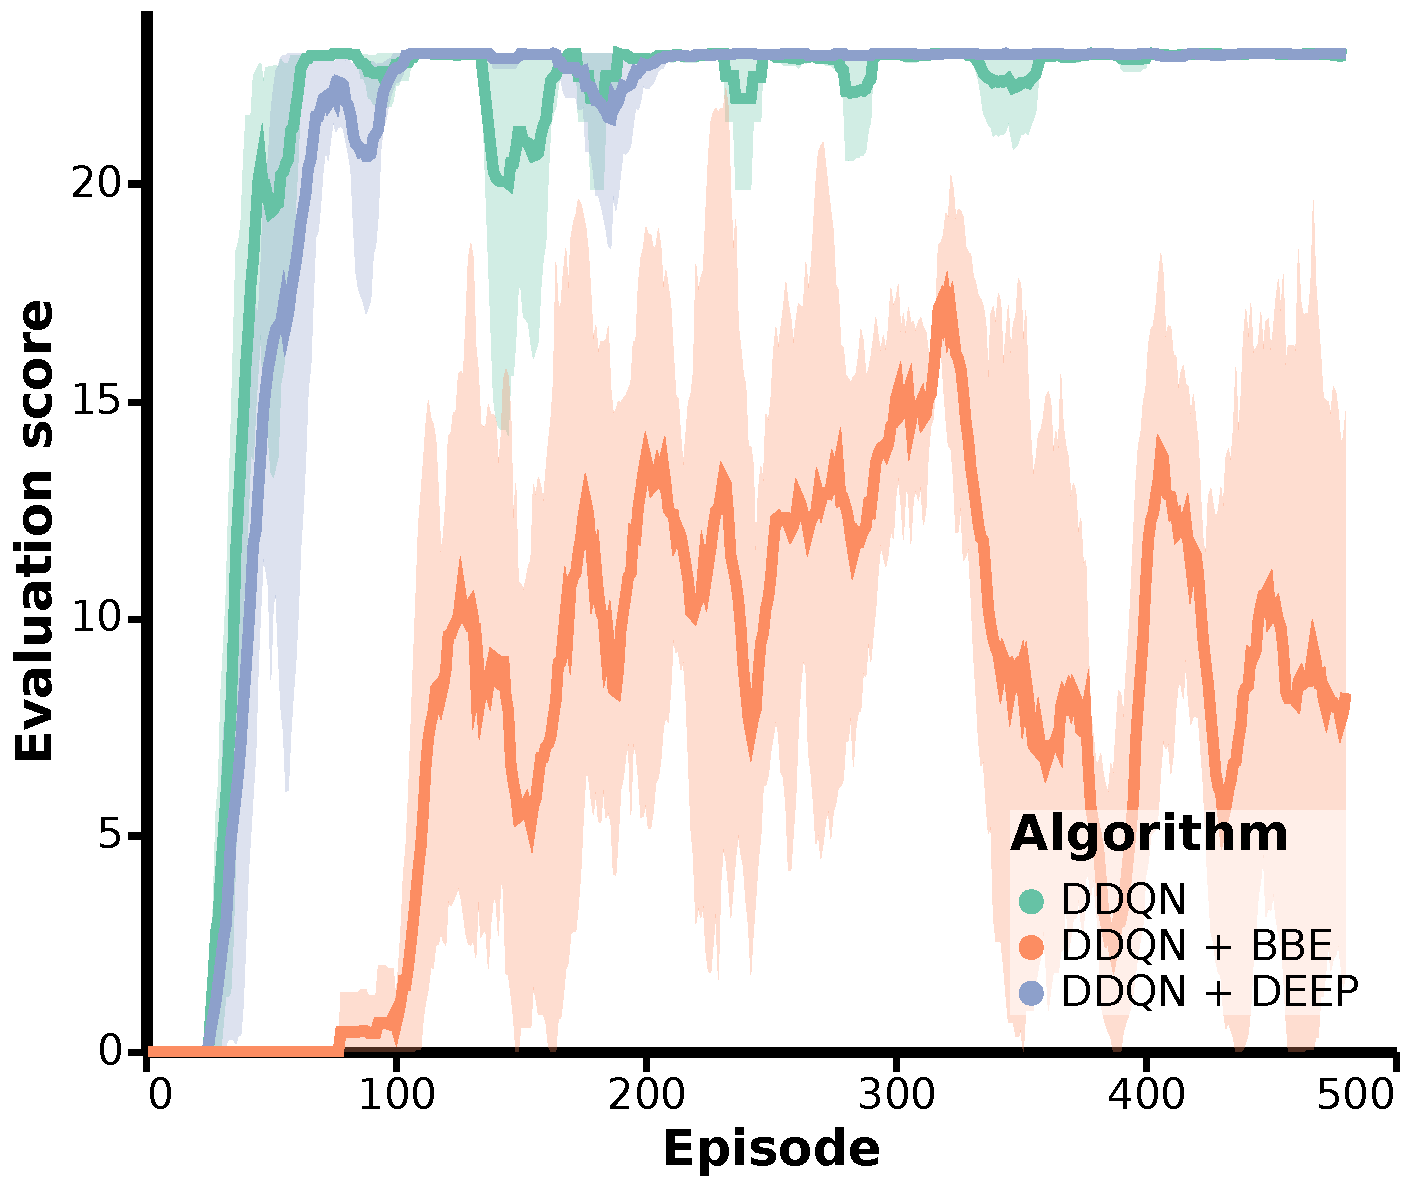
\includegraphics[width=0.8\textwidth]{figures/deep/grid40_warmstart.pdf}
        \caption{Reward}
    \end{subfigure}
    \hfill
    \begin{subfigure}[b]{0.49\textwidth}
        \centering
        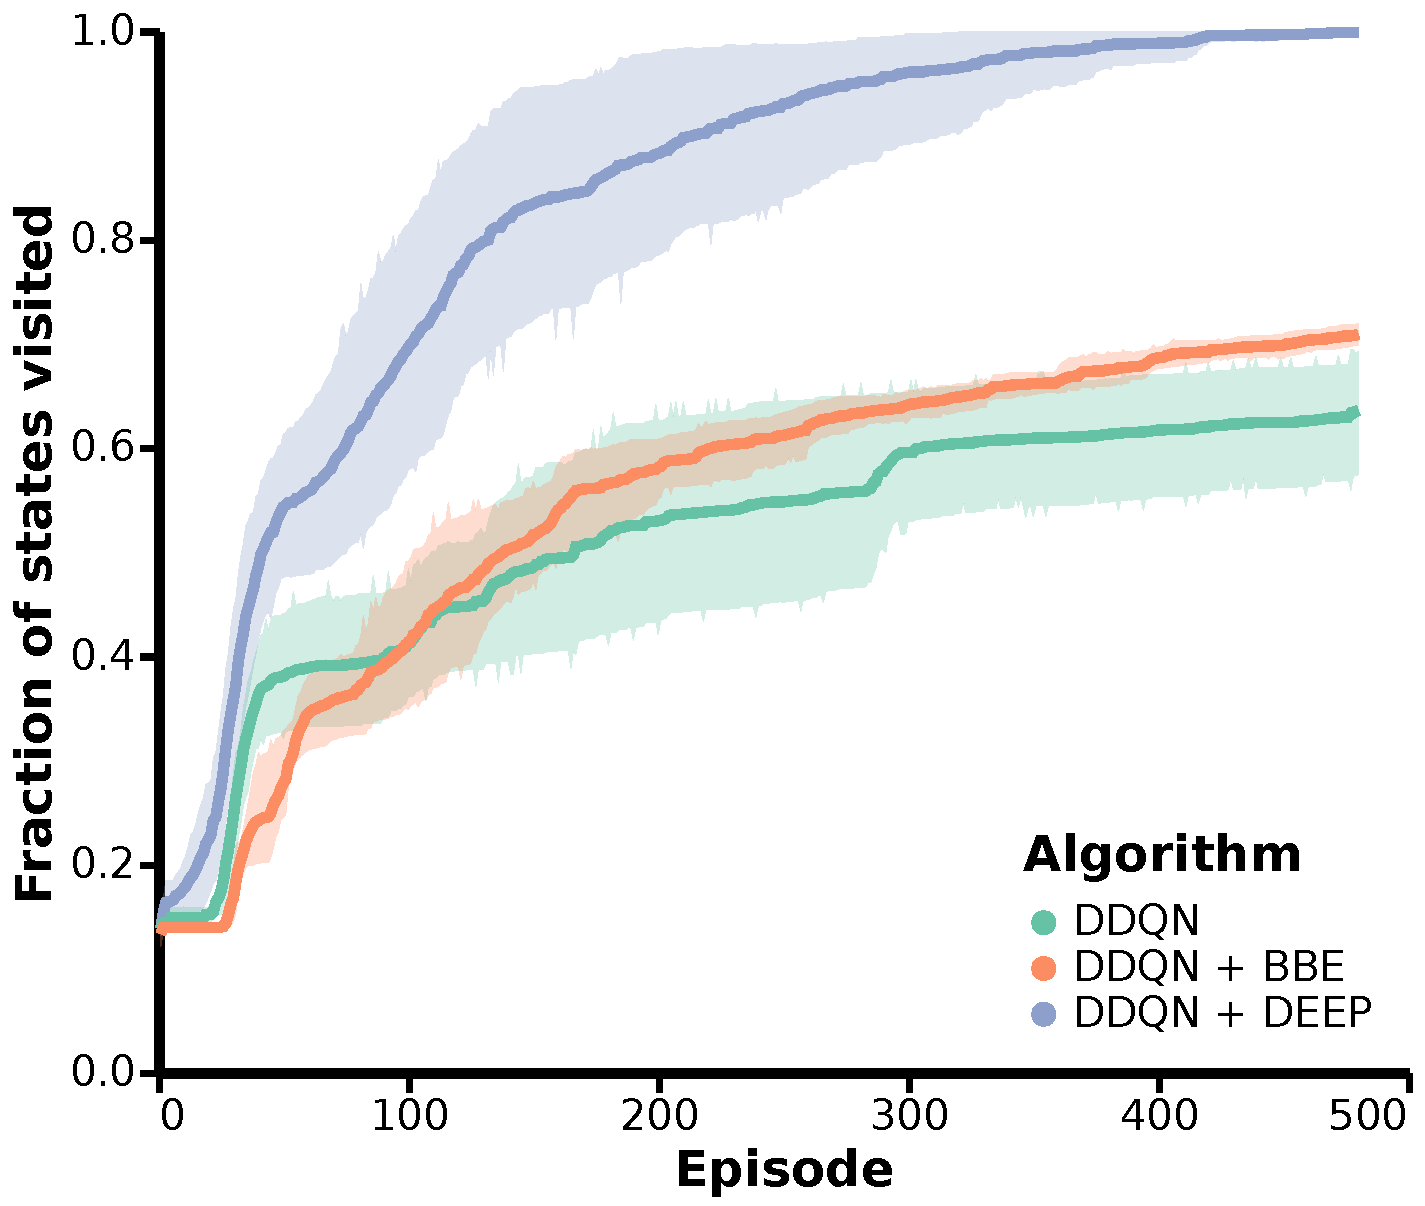
\includegraphics[width=0.8\textwidth]{figures/deep/grid40_warmstart_visits.pdf}
        \caption{Coverage}
    \end{subfigure}
    \caption{Experiments in a $40 \times 40$ grid-world environment with one goal state, where learning algorithms were warm-started with 20 episodes of data from a skilled policy.
    \textbf{(a)} With enough signal to find the goal, DDQN (Double DQN, \citet{Hasselt2016DeepRL}) alone rapidly converges to the optimal policy. BBE introduces bias, causing the policy to continually explore. Our method, \algshort{}, learns the task policy just as rapidly as DDQN alone.
    \textbf{(b)} Though it performs well, DDQN simply goes to the goal during each train episode and does not explore other options. BBE continues to seek out new states at a slow but steady rate. \algshort{} explores far more than BBE during data collection despite simultaneously performing just as well as DDQN at evaluation time.}
    \label{fig:gridworld_warmstart}
\end{figure}

The bonus-based exploration algorithm, illustrated in \Cref{alg:bbe}, has two weaknesses which limit its usefulness for sample-efficient policy learning.


\paragraph{Bias with finite samples.}
Because they estimate the optimal policy on the modified MDP $\mdp'$, bonus-based exploration algorithms learn biased policies as long as the exploration bonus is nonzero.
According to theory, the exploration bonus should be scaled larger than is done in practice \citep{strehl2008analysis} and decay slower than $\nicefrac{1}{N(s)}$ \citep{Kolter2009NearBayesianEI} in order to guarantee convergence to the optimal policy.
This behavior, shown in \Cref{fig:gridworld_warmstart}, can result in slow convergence to the optimal policy and substantially biased policies after a practically feasible number of samples.

\begin{figure}[h]
    \begin{center}
        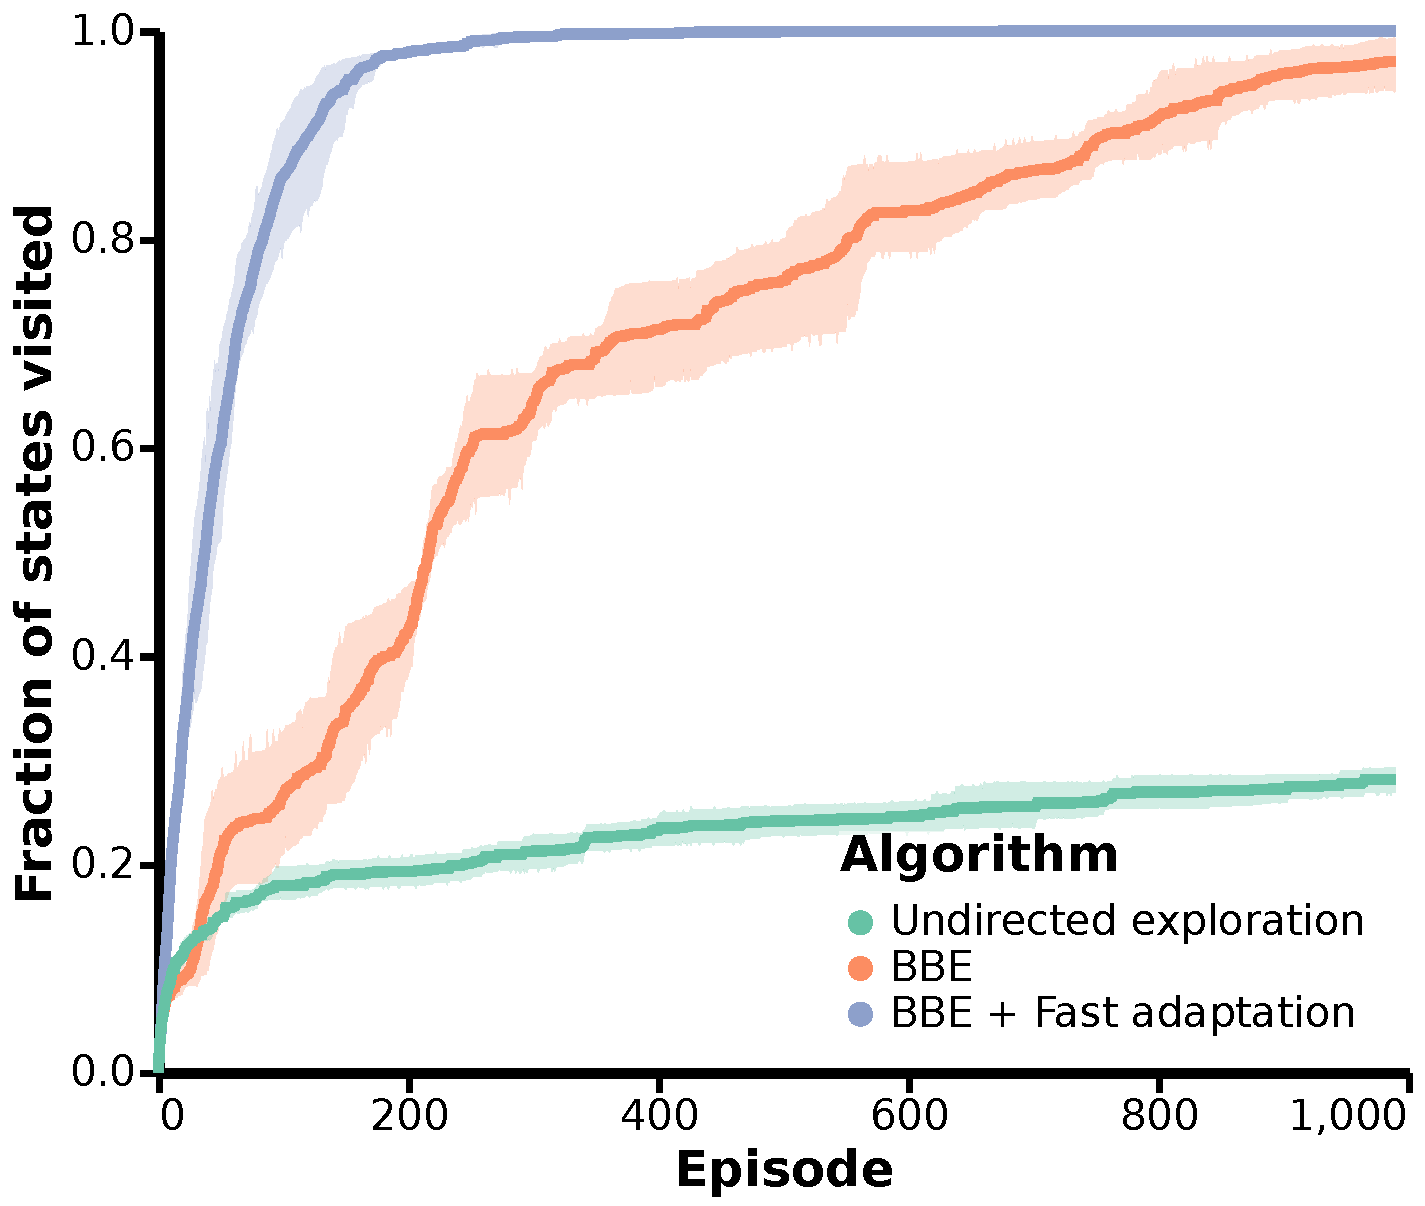
\includegraphics[width=0.35\textwidth]{figures/deep/grid40_visits_neurips.pdf}
    \end{center}
    % \caption{A test of pure exploration speed. Undirected exploration with a uniformly random policy covers the state space very slowly. BBE, with its ability to seek unknown states, is faster. However, BBE does not adapt rapidly to the changing rewards, leading it to be slower than the fast adaptation scheme we propose.}
    \caption{Pure exploration}
    \label{fig:gridworld_visits}
\end{figure}

% \caption{Two experiments in a $40 \times 40$ grid-world environment with one goal state. \textbf{(a)} Learning algorithms warm-started with 20 episodes of data from a skilled policy. Since there is plenty of signal to find the goal, DDQN without exploration rapidly converges to the optimal policy. BBE introduces bias, causing the policy to continually explore. Our method, \algshort{}, learns the task policy just as rapidly as DDQN alone.
% \textbf{(b)} A test of pure exploration speed. Undirected exploration with a uniformly random policy covers the state space very slowly. BBE, with its ability to seek unknown states, is faster. However, BBE does not adapt rapidly to the changing rewards, leading it to be slower than the fast adaptation scheme we propose.\textcolor{red}{TOBI: TODO these need to take the count function/bonus reward as input and update them.}}


\paragraph{Slow adaptation to changing rewards.}
Algorithms in this family update the policy according to the schedule of the underlying model-free RL algorithm -- for example at the end of each episode.
This works well for the stationary MDPs that these algorithms were developed for, but the modified MDP $\mdp'$ which represents the exploration problem is non-stationary.
This leads to an agent which determines the most novel state and then stays there for an entire episode.
This degenerate behavior leads to potentially exploring only a single state per episode instead of visiting a sequence of new states as the reward function evolves.\endnote{Some implementations of bonus-based exploration may update the policy within an episode, for example via a single gradient step per environment step on transitions sampled i.i.d.~from a replay.
However, such a small update is typically not enough to change the qualitative behavior of the agent and adapting to the changing MDP has not been an emphasis in prior work.}
The use of replay buffers compounds this effect, since algorithms in this family compute exploration rewards at the time the transition is collected, rather than when it is used.
An algorithm which is unaware of the non-stationary nature of the MDP will maximize the return on this mixture of reward functions rather than the reward that incorporates the current bonus, resulting in slow coverage of the environment.
\Cref{fig:gridworld_visits} shows uniform random actions, BBE, and BBE with the fast adaptation scheme we propose in \Cref{sec:fast_adaptation} all exploring in a $40 \times 40$ grid-world without rewards.
While BBE covers the state space much faster than undirected exploration, it is unnecessarily slow.
See Appendix \ref{sec:gridworld-vis} for visualizations.


\section{Decoupled exploration for sample-efficient control}
In this section, we describe a new algorithm called \algname{} (\algshort{}) which addresses the limitations of BBE.
The core insight is that by leveraging off-policy RL algorithms, \algshort{} can learn two policies from the same replay: a task policy $\pitask$, which maximizes the reward on the original MDP $\mdp_R$, and an exploration policy $\piexplore$, which maximizes only the reward on the bonus MDP $\mdp_{R^+_n}$.
This decoupling serves two purposes.
First, it enables good performance even before exploration is complete by using $\pitask$ at test time.
Second, it allows $\piexplore$ to be updated aggressively in order to more closely match the non-stationary bonus MDP; unlike $\pitask$, it is not important that $\piexplore$ converge exactly to an optimal policy.

Like BBE, \algshort{} is a family of algorithms related by their structure; a particular algorithm in this family consists of a choice of an exploration reward function and an off-policy RL algorithm for learning each policy.
Throughout this work, we use a pseudo-count based exploration reward.
For discrete tasks we use Double DQN (DDQN, \citet{Hasselt2016DeepRL}) and Boltzmann policies.
For tasks with continuous actions we use soft actor-critic (SAC) for $\pitask$ and a DDQN policy for $\piexplore$.


\subsection{Pseudo-count estimation} \label{sec:kernel_counts}
Following \citet{bellemare2016unifying}, we use an exploration reward derived from pseudo-counts.
Instead of the high-dimensional pixel observations of the ALE, Control Suite has low-dimensional ($<$100-D) observations corresponding to joint and object locations and velocities.
% This allows us to replace the pseudo-counts extracted from a density estimator used in that work with a directly specified pseudo-count function based on kernels.
This lower dimensionality renders extracting pseudo-counts from a density estimator unnecessary, and in our experiments we specify a pseudo-count function based on kernels.
For a real-valued state-action pair $x = [s, a]$ and a set of previous observations $\{x_i\}_{i=1}^n$, define the pseudo-count of $x$ and the exploration reward as
\begin{align}
    \hat N_n(x) = \sum_{i=1}^n k(x_i, x) && R^+_n(s, a) = \hat N_n \big([s, a] \big)^{-1/2}
\end{align}
where $k$ is a kernel function scaled to have a global maximum $k(x, x) = 1$.
This satisfies the key requirement for a pseudo-count function, namely that a visit to a state $x$ increases $\hat N(x)$ by 1 and $\hat N(x')$ by at most 1 for any other state $x'$.
In our experiments we use a Gaussian kernel (scaled to have a maximum value of 1) with diagonal covariance.
For implementation details see Appendix \ref{sec:count_implementation}.
% \todo{write the actual reward function}

\subsection{Separating task and exploration policies}

\algshort{} uses two separate policies.
Each is trained off-policy using transitions sampled from the replay buffer; $\pitask$ is updated using the rewards from $R$ logged in the replay, while $\piexplore$ is updated using rewards from $R^+_n$.
Since $\pitask$ is trained only on the rewards for the true task, it is unbiased in the sense that it reflects the current best estimate of the optimal policy.
This stands in contrast to BBE policies, which optimize the sum of task and exploration rewards and thus represent a biased estimate of the optimal task policy until the exploration rewards go to zero.
Our method is agnostic to the choice of algorithm and policy parameterization.
However, it will be most effective with policy learning algorithms that work well when trained far off-policy and produce high-entropy policies (e.g. policies which cover all optimal actions).
For these reasons we use the state-of-the-art maximum-entropy algorithm SAC to learn $\pitask$ in environments with continuous actions. For experiments with discrete action spaces we forego explicitly learning the task policy $\pitask$; instead we learn the task Q-function via DDQN \citep{Hasselt2016DeepRL} and define the task policy as $\pitask(a | s; Q) \propto \exp(Q(s, a) / \tau)$, where $\tau > 0$ becomes a hyperparameter -- we refer to the supplementary material for details.


\subsection{Fast-adapting exploration policy} \label{sec:fast_adaptation}
The non-stationary nature of the exploration reward function poses a challenge to typical model-free RL algorithms, which assume a fixed reward function.
BBE methods update a single policy using a replay buffer which, at a step $n$, contains rewards from a mixture of bonus reward functions $\{R_1^+, \ldots, R_n^+\}$, computed using different past novelty or count estimates.\endnote{See e.g. the code from \citet{Machado2020CountBasedEW}:  \url{https://github.com/mcmachado/count_based_exploration_sr/blob/master/function_approximation/exp_eig_sr/train.py\#L204}}
This results in slow adaptation to the non-stationary objective of exploration.
\algshort{} makes two changes to mitigate the impact of the non-stationarity in the exploration reward function.

First, \algshort{} leverages access to $R^+_n$ to compute exploration rewards when they are needed to update $\piexplore$ rather than when the transition is collected.
We choose to use Q-learning rather than a more sophisticated algorithm in order to learn $\piexplore$ as rapidly as possible; with changing rewards, using a policy to amortize the maximization of a value function as in SAC or DDPG would slow down learning.
We represent $\piexplore$ directly as a Boltzmann policy of this exploration Q-function $\qex$:
\begin{align}
    \piexplore(a \mid s) \propto \exp \left\{ \frac{\qex(s, a)}{\tex} \right\},
\end{align}
where $\tex$ is a temperature hyperparameter.

Second, by decoupling $\piexplore$ from $\pitask$, \algshort{} unlocks the ability to update $\piexplore$ more aggressively without affecting $\pitask$'s convergence to the optimal policy.
This enables the exploration policy to more rapidly adapt to the non-stationary exploration reward.
In our experiments we achieve this by using a larger learning rate and more updates per environment step than is usually done; future work might investigate more sophisticated schemes such as prioritized sweeping \citep{Moore1993PrioritizedSR} or prioritized experience replay \citep{Schaul2016PrioritizedER}.
To improve stability we use DDQN updates and clip Q targets at $\bar{r}$, the maximum discounted exploration value.
% \todo{discuss clipping targets at 100?}

\paragraph{Optimism.} \label{sec:optimistic}
Further adapting $\piexplore$ to the unique properties of the exploration reward function, we propose to leverage optimism in its updates and actions.
We propose to make $\qex$ optimistic by leveraging the pseudo-count function in a manner similar to that proposed by \citet{Rashid2020OptimisticEE}.
We assume that the value function is trustworthy for transitions with very large counts, and very untrustworthy for transitions with near-zero counts.
When the count is zero we impose an optimistic prior which assumes the transition will lead to a whole episode of novel transitions; as the count increases we interpolate between this prior and the learned value function using a weighting function:
\begin{align} \label{eq:optimism}
\qex^+(s, a) = w(s, a) \cdot \qex(s, a) + (1 - w(s, a))  \cdot \bar{r}, \qquad w(s, a) = \frac{\sqrt{N(s, a)}}{\sqrt{N(s, a) + c}}
\end{align}
where $\bar{r} = \nicefrac{1}{1-\gamma}$, is the maximum discounted return in the bonus MDP and $c$ is a small constant representing how many counts' worth of confidence to ascribe to the optimistic prior.
We use this optimistic $\qex^+$ for computing targets for Bellman updates and for computing $\piexplore$ (Eq. \ref{eq:behavior_policy}).
For details of the implementation of the fast-adapting $\piexplore$, see Appendix \ref{sec:fast_updates_appendix}.


\subsection{Product distribution behavior policy}
A good behavior policy should attempt to explore all of the transitions which are relevant for learning the optimal policy.
This entails a trade-off between taking actions which are more novel and ones which are more likely to be relevant to a high-performing policy.
\algshort{} encodes this by representing the behavior policy as a product of the task policy $\pitask$ and the pure-exploration policy $\piexplore$:
\begin{align} \label{eq:behavior_policy}
\beta(a \mid s) \propto \pitask(a \mid s) ~ \piexplore(a \mid s).
\end{align}
% where $\tex$ is a temperature hyperparameter controlling the aggressiveness of the exploration and $\qex^+$ is an optimistic version of the exploration value function (see \Cref{sec:optimistic}).

The choice to parameterize $\beta$ as a factored policy was made for its simplicity and ease of off-policy learning.
Alternative formulations for making this trade-off while preserving the unbiased task policy are possible, and we view the form of our proposed behavior policy as just one option among many.
One alternative would be interleaving the behavior of multiple policies within one episode, akin to e.g. Scheduled Auxiliary Control \citep{Riedmiller2018LearningBP}.

In order to approximately sample from this behavior policy, we use self-normalized importance sampling with $\pitask$ as the proposal distribution:
\begin{enumerate}
    \item Draw $k$ samples $a_1, \ldots, a_k$ from $\pitask$
    \item Evaluate $\piexplore(a_i \mid s)$ for each $i \in 1 \ldots k$
    \item Draw a sample from the discrete distribution $p(a_i) = \piexplore(a_i \mid s) / \sum_{i'} \piexplore(a_{i'} \mid s)$.
\end{enumerate}
Note that since the proposal distribution is $\pitask$, the $\pitask$ terms in computing weights cancel and only the $\piexplore$ terms remain.
Importance weighting is consistent in the limit of $k \to \infty$ but introduces bias towards $\pitask$ \citep{Vehtari2015ParetoSI}.
With small $k$, this bias makes it unlikely that $\beta$ will select actions that are very unlikely under $\pitask$; roughly speaking, this procedure selects the ``most exploratory'' action in the support of the task policy.
This may act as a backstop to prevent the behavior from going too far outside the task policy to be useful.
\algshort{} works best when $\pitask$ is trained in a way that preserves variance in the policy (e.g. SAC's target entropy), enabling the behavior policy to select exploratory actions. In discrete action spaces we additionally use self-normalized importance sampling -- using a uniform proposal over actions -- to obtain samples from $\pitask$ in step 1.
% and \algshort{} with a deterministic task policy would .

% If the RL algorithm for learning $\pitask$
% If the RL algorithm for learning $\pitask$
% As mentioned above, this procedure works best when $\pitask$ is trained in a way that preserves variance in the policy (e.g. by enforcing a minimum entropy in the policy).
% If the choice of RL algorithm does not give such a guarantee importance sampling based on a mix of a random proposal and the task policy could be performed.


\section{Experiments}
% \red{Goals: (1) show that BBE hurts on dense environments, and ours doesn't; (2) show that ours learns fastest on spare environments}

In this section we perform experiments to give insight into the behavior of undirected exploration, BBE, and \algshort{}.
% In particular, we investigate how each algorithm's performance changes as the task requires more exploration
First we perform a set of investigative experiments to probe how \algshort{} interacts with environments with different reward structures.
Then we perform experiments on pairs of benchmark continuous control tasks with easy and hard exploration requirements.

\begin{figure}[h]
    \centering
    \begin{subfigure}[b]{0.49\textwidth}
        \centering
        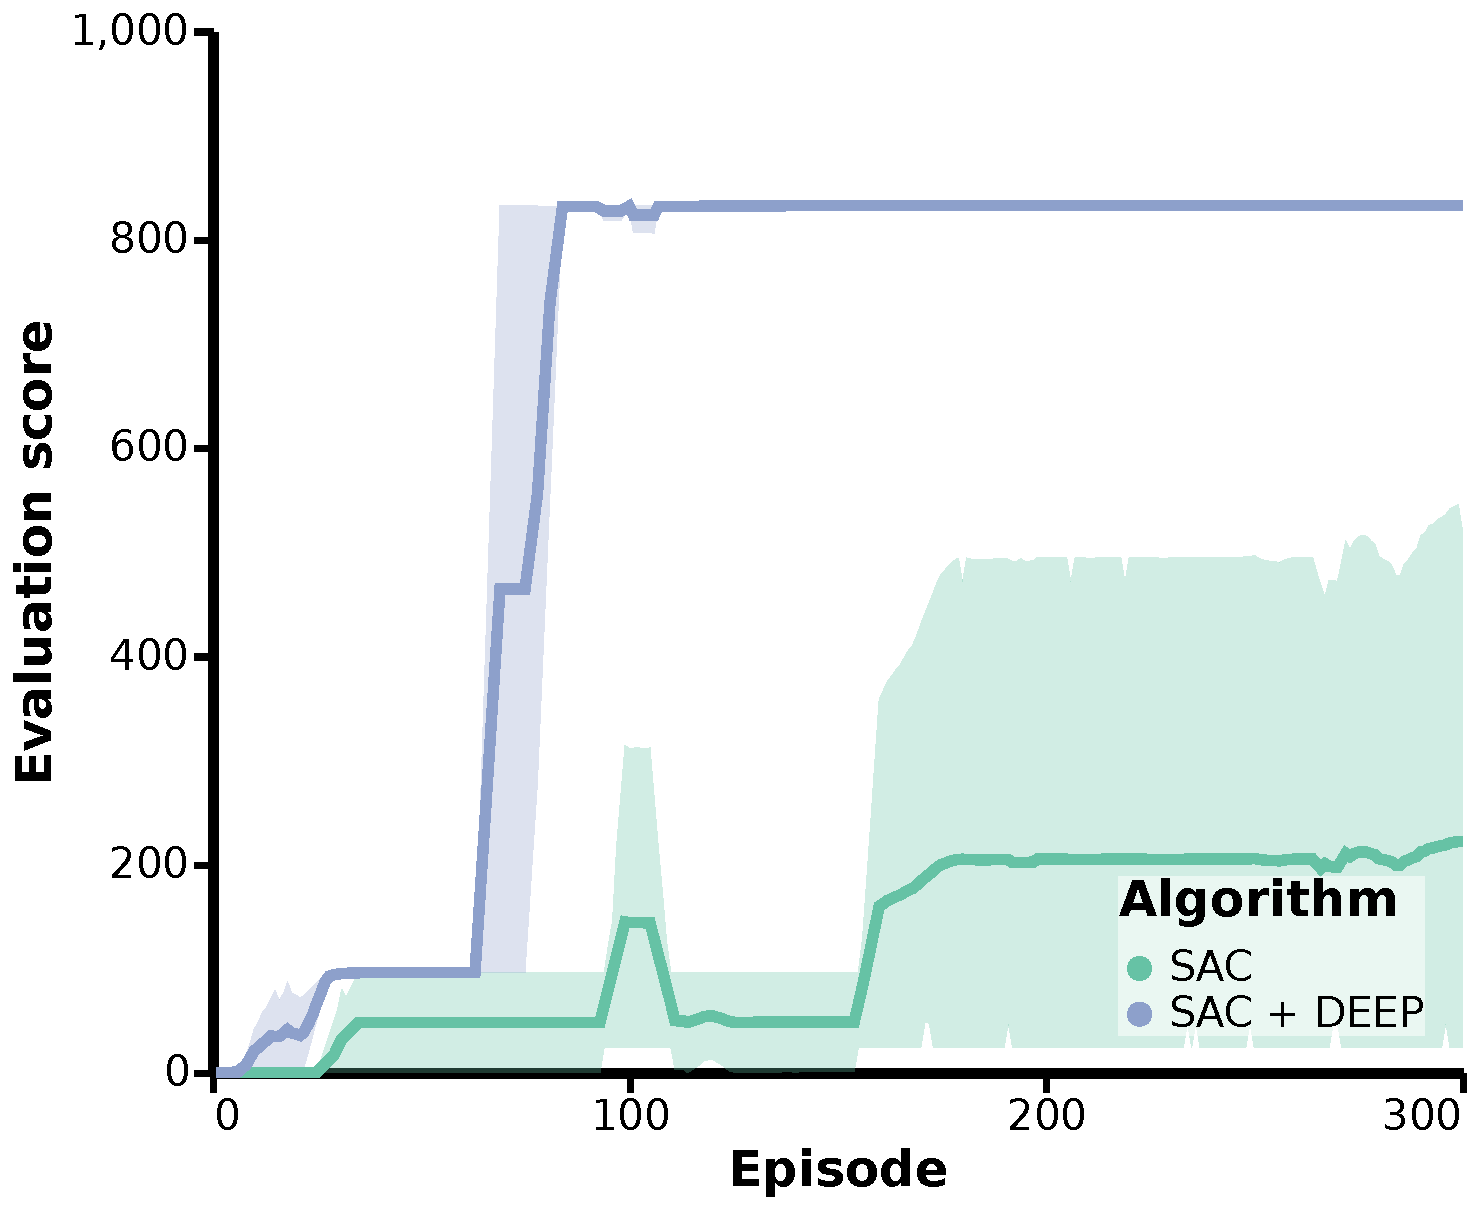
\includegraphics[width=0.8\textwidth]{figures/deep/hallway_velocity_4_distractor.pdf}
        \caption{Local optimum environment} \label{fig:hallway_local_optimum}
    \end{subfigure}
    \hfill
    \begin{subfigure}[b]{0.49\textwidth}
        \centering
        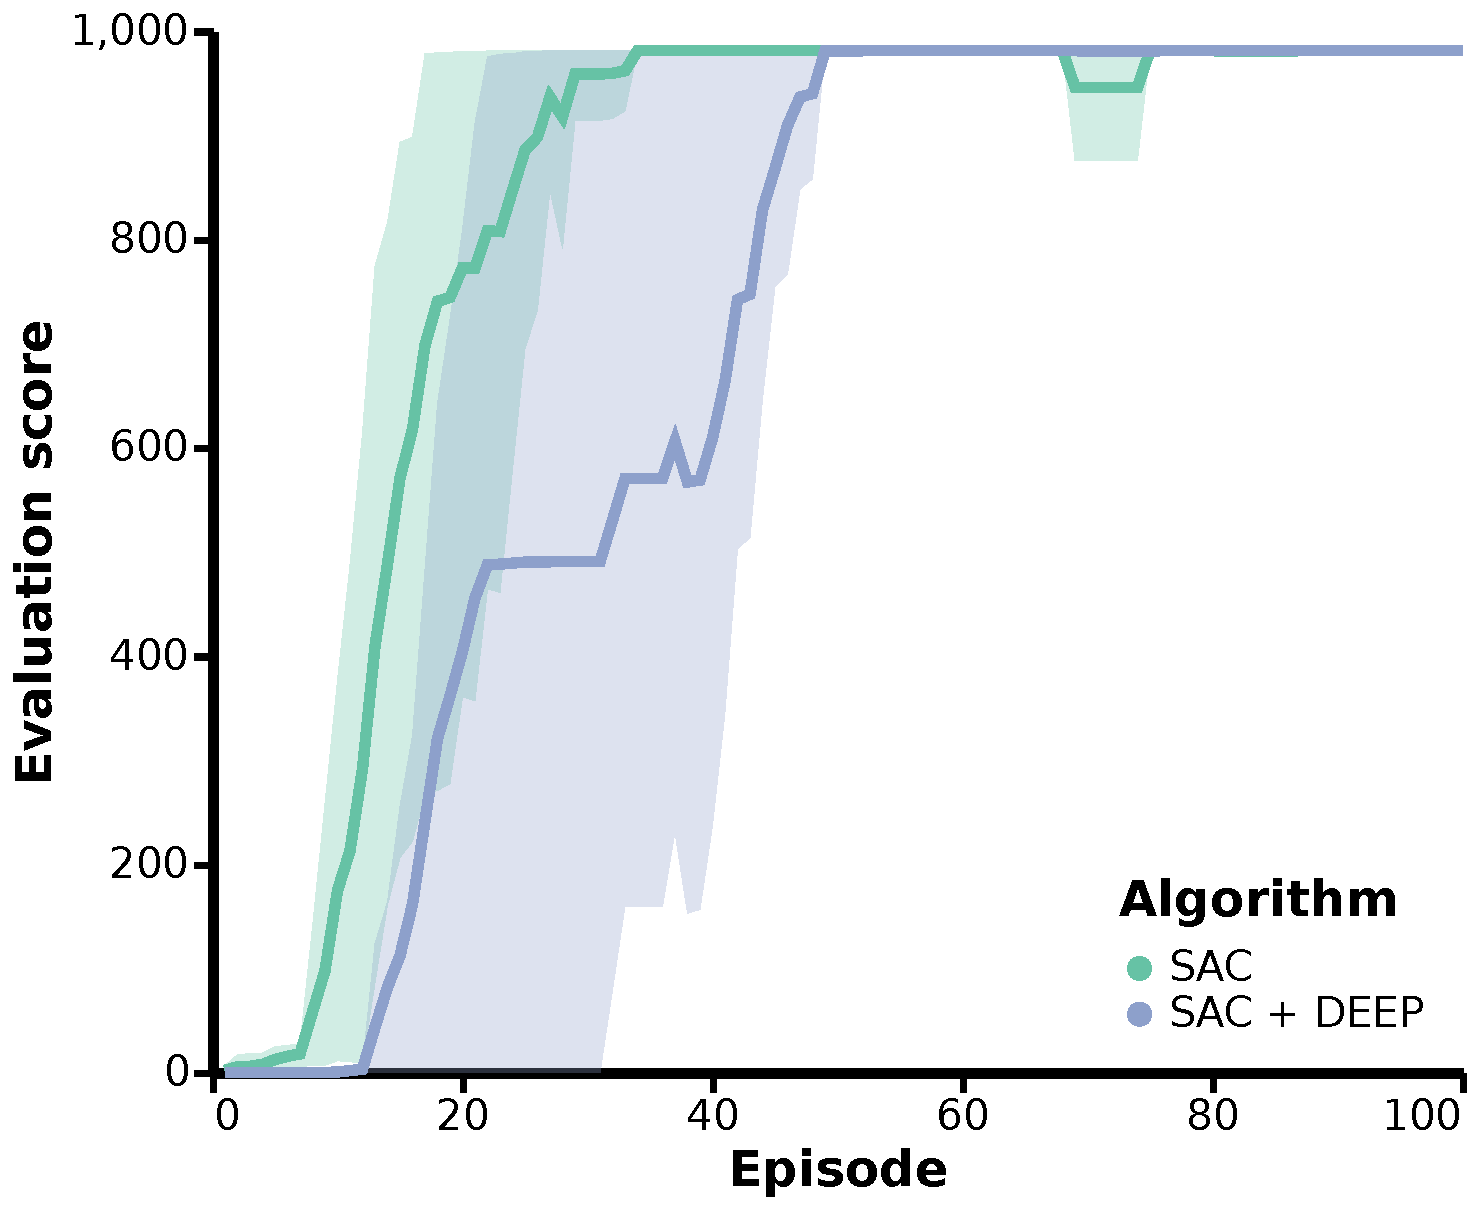
\includegraphics[width=0.8\textwidth]{figures/deep/hallway_velocity_4_inverse_distractor.pdf}
        \caption{Adversarial environment}\label{fig:inverse_distractor}
    \end{subfigure}
    \caption{Two environments illustrating different reward structures.
    \textbf{(a)} An environment with a locally-optimal goal (reward 0.1) near the start state. SAC finds this nearby goal, but doesn't explore far enough to find the real goal (reward 1.0). When trained with \algshort{}, it finds the distractor goal but moves on to the real goal.
    \textbf{(b)} An adversarial environment for \algshort{} which has a very small goal state close to the start state, making it easy to find with random actions but hard with directed exploration.}
    \label{fig:hallway}
\end{figure}

\subsection{Investigative experiments}

We construct a simple MuJoCo \citep{todorov2012mujoco} environment called Hallway to look more closely at how exploration interacts with reward structure.
This environment consists of a long narrow 2D room with the agent controlling the velocity of a small sphere, which starts each episode at one end of this hallway.
The following two experiments share dynamics and differ only in their rewards.

\paragraph{Local optima.}
A valuable role for exploration is enabling an agent to escape from locally optimal behavior.
% behavior that is locally but not globally optimal.
To test this, we add two goal states with shaped rewards to the Hallway environment.
The first is close to the start state but only provides reward at most 0.1, while the second is at the far end of the hallway but provides reward 1.0.
\Cref{fig:hallway_local_optimum} shows that exploration using \algshort{} allows the agent to quickly find its way to the faraway optimal reward while SAC gets stuck in the local optimum.


\paragraph{Limitations.}
% While \algshort{} outperforms SAC in each of the Control Suite environments, there is no such thing as a universally optimal exploration strategy.
\algshort{} covers states quickly, but there is no such thing as a universally optimal exploration strategy.
For example, there exist environments for which the random walk dynamics of undirected exploration find the optimal strategy faster than uniform state coverage.
\Cref{fig:inverse_distractor} provides one such example: a Hallway environment with a very small goal state close to the start state.
SAC discovers this goal faster than SAC + \algshort{}, though \algshort{} does eventually find it as well.


\subsection{Benchmark experiments}
Next we provide experiments based on DeepMind Control Suite \citep{tassa2018deepmind}, a standard benchmark for continuous control RL algorithms.
We introduce versions of several environments which are modified to remove the accommodations that make them solvable without exploration, then provide results of SAC, SAC + BBE, and SAC + \algshort{} on the original and modified environments.

\subsubsection{Results}
\begin{figure}[ht]
    \centering
    \begin{subfigure}[b]{0.24\textwidth}
        \centering
        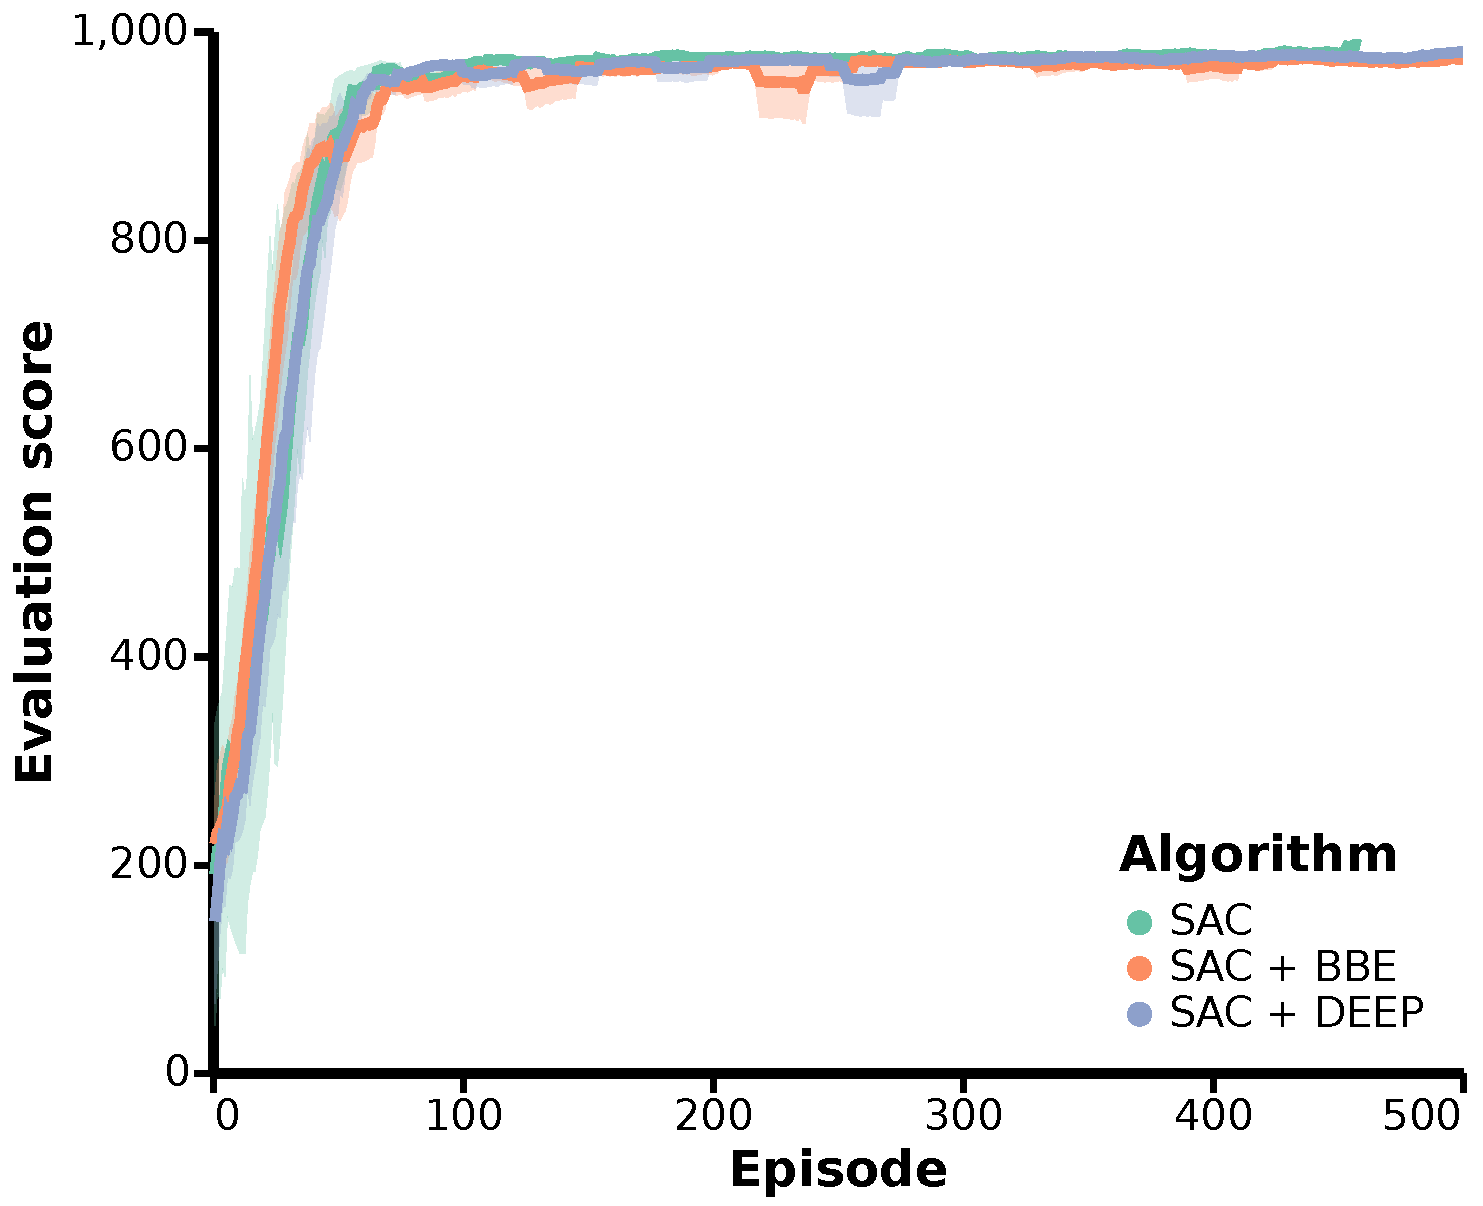
\includegraphics[width=\textwidth]{figures/deep/neurips_ball_in_cup.pdf}
        \caption{Ball-in-cup}
    \end{subfigure}
    \begin{subfigure}[b]{0.24\textwidth}
        \centering
        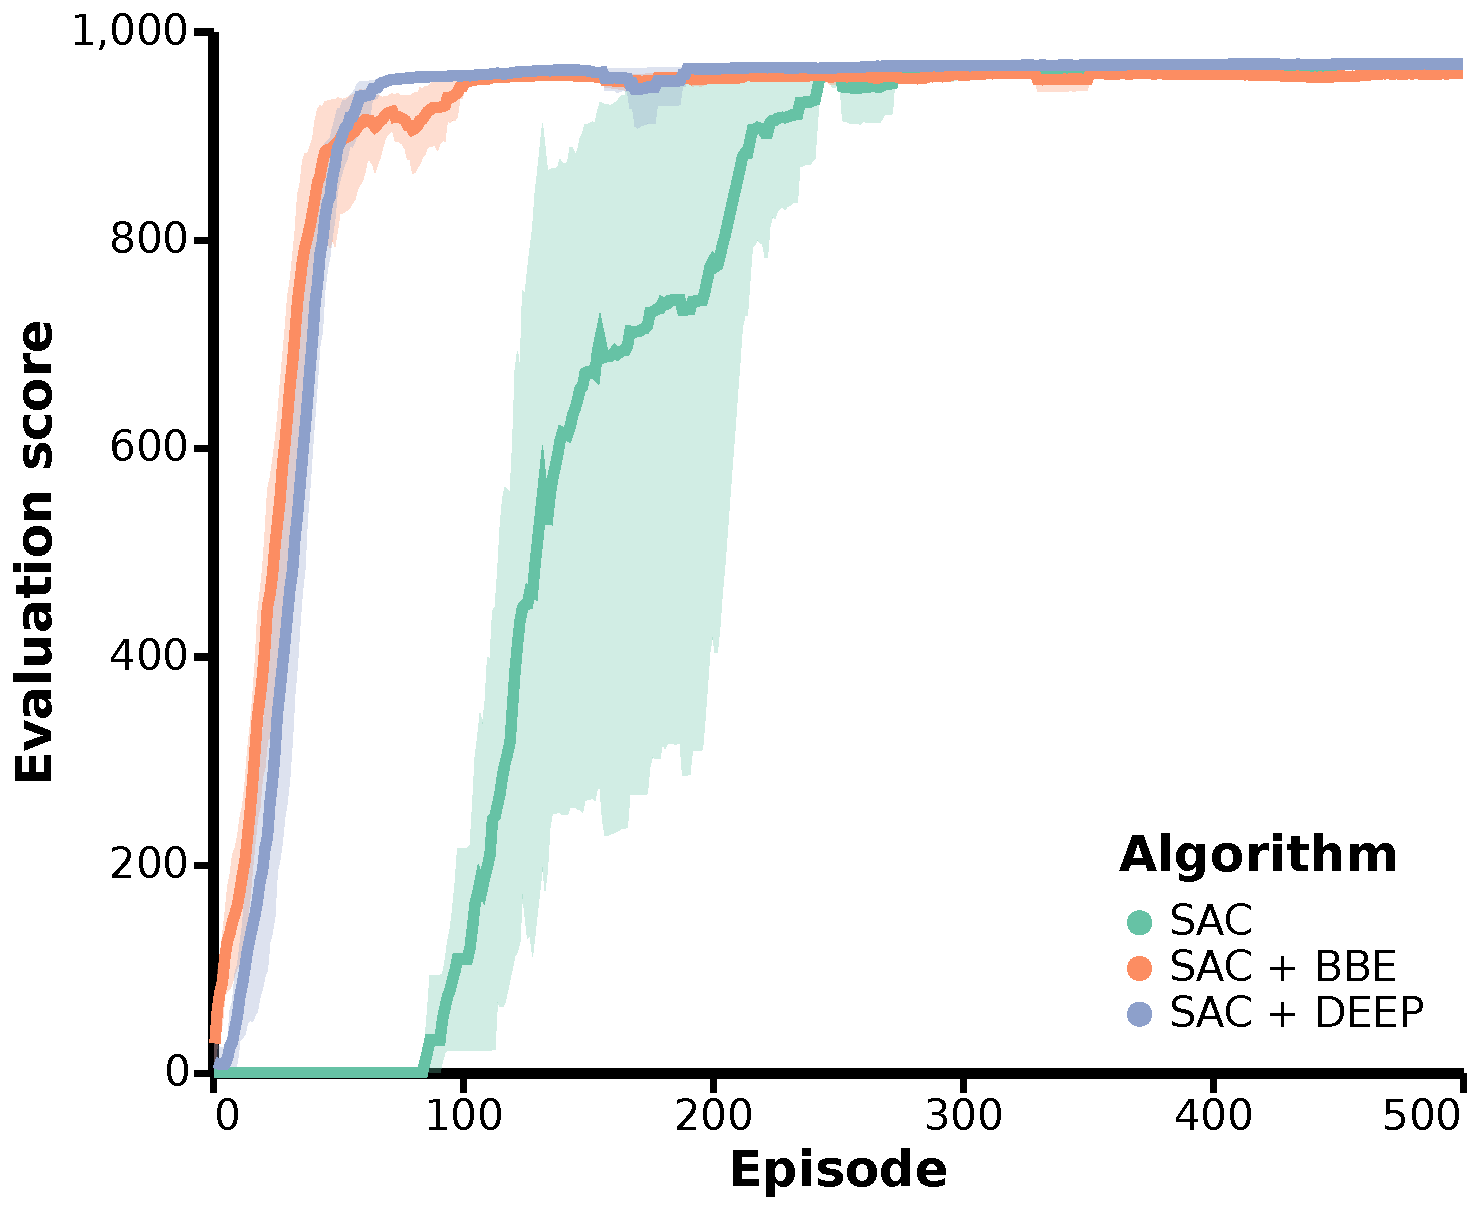
\includegraphics[width=\textwidth]{figures/deep/neurips_ball_in_cup_explore.pdf}
        \caption{Ball-in-cup explore}
    \end{subfigure}
    % \caption{Adding \algshort{} does not result in worse performance on the original ball-in-cup environment. In a version of the environment with resets that do not provide full coverage, \algshort{} performs just as well, whereas the performance of plain SAC is greatly impaired.}
    % \label{fig:ball_in_cup}
    \hfill
    \begin{subfigure}[b]{0.24\textwidth}
        \centering
        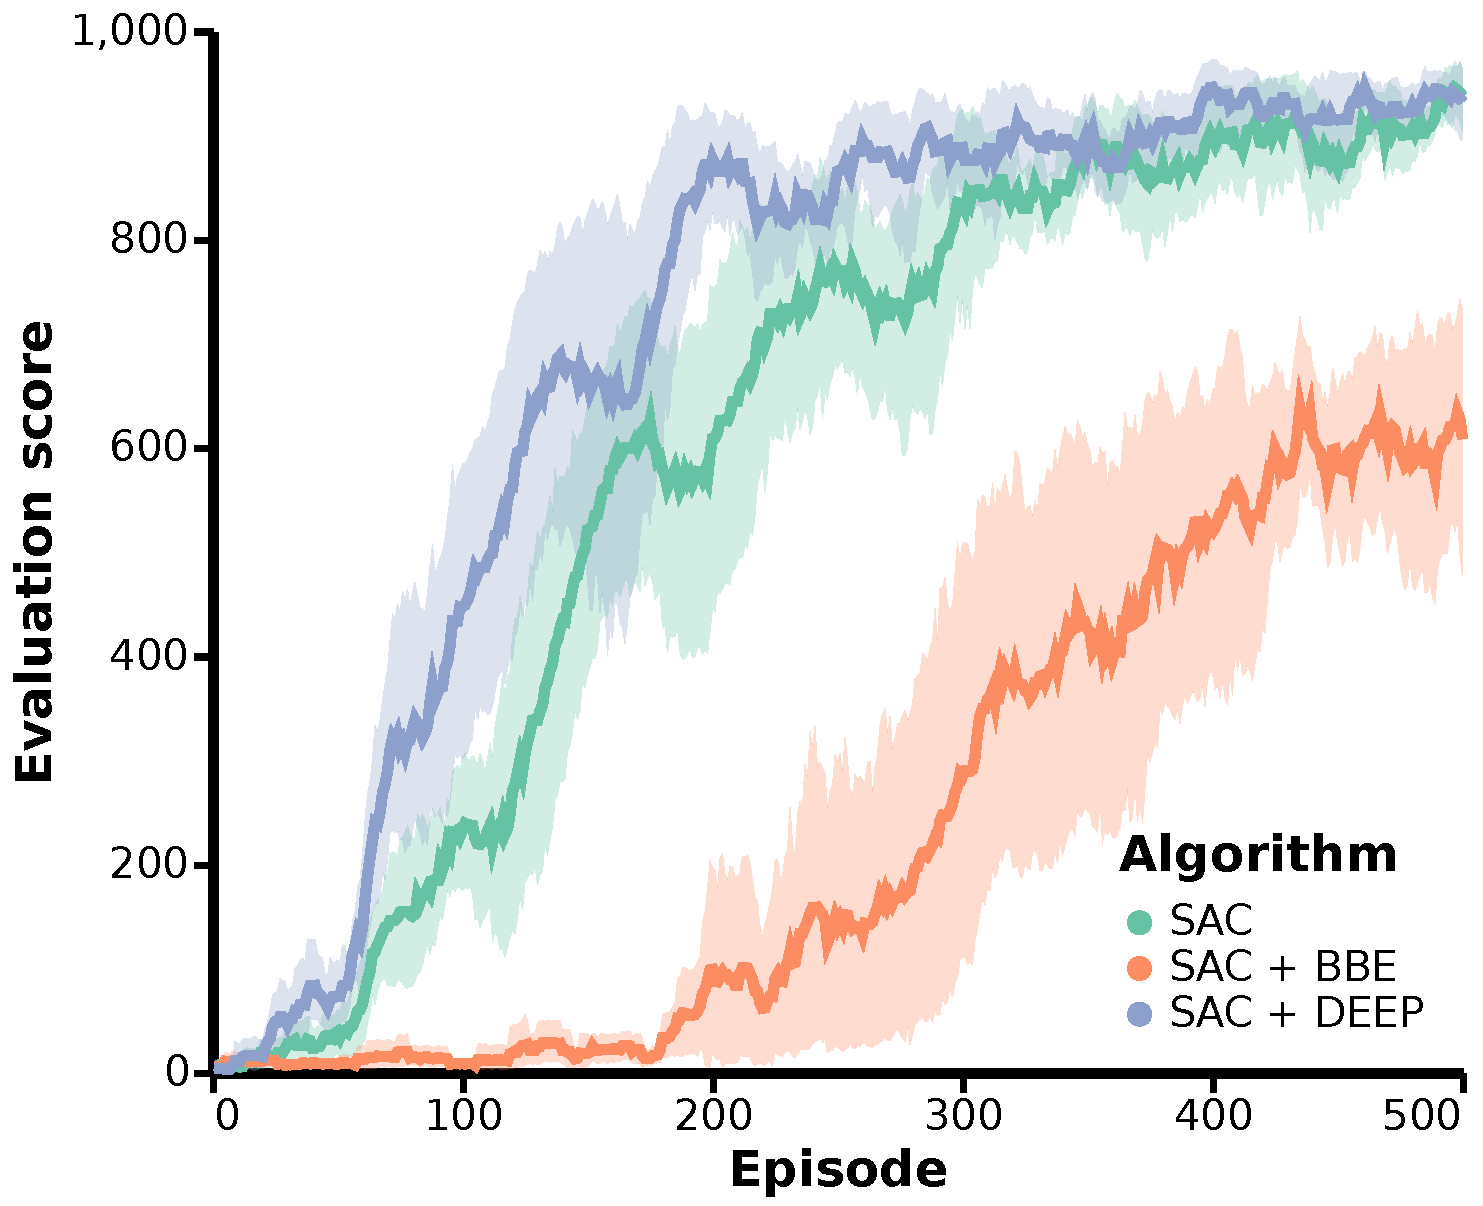
\includegraphics[width=\textwidth]{figures/deep/neurips_reacher.pdf}
        \caption{Reacher}
    \end{subfigure}
    \begin{subfigure}[b]{0.24\textwidth}
        \centering
        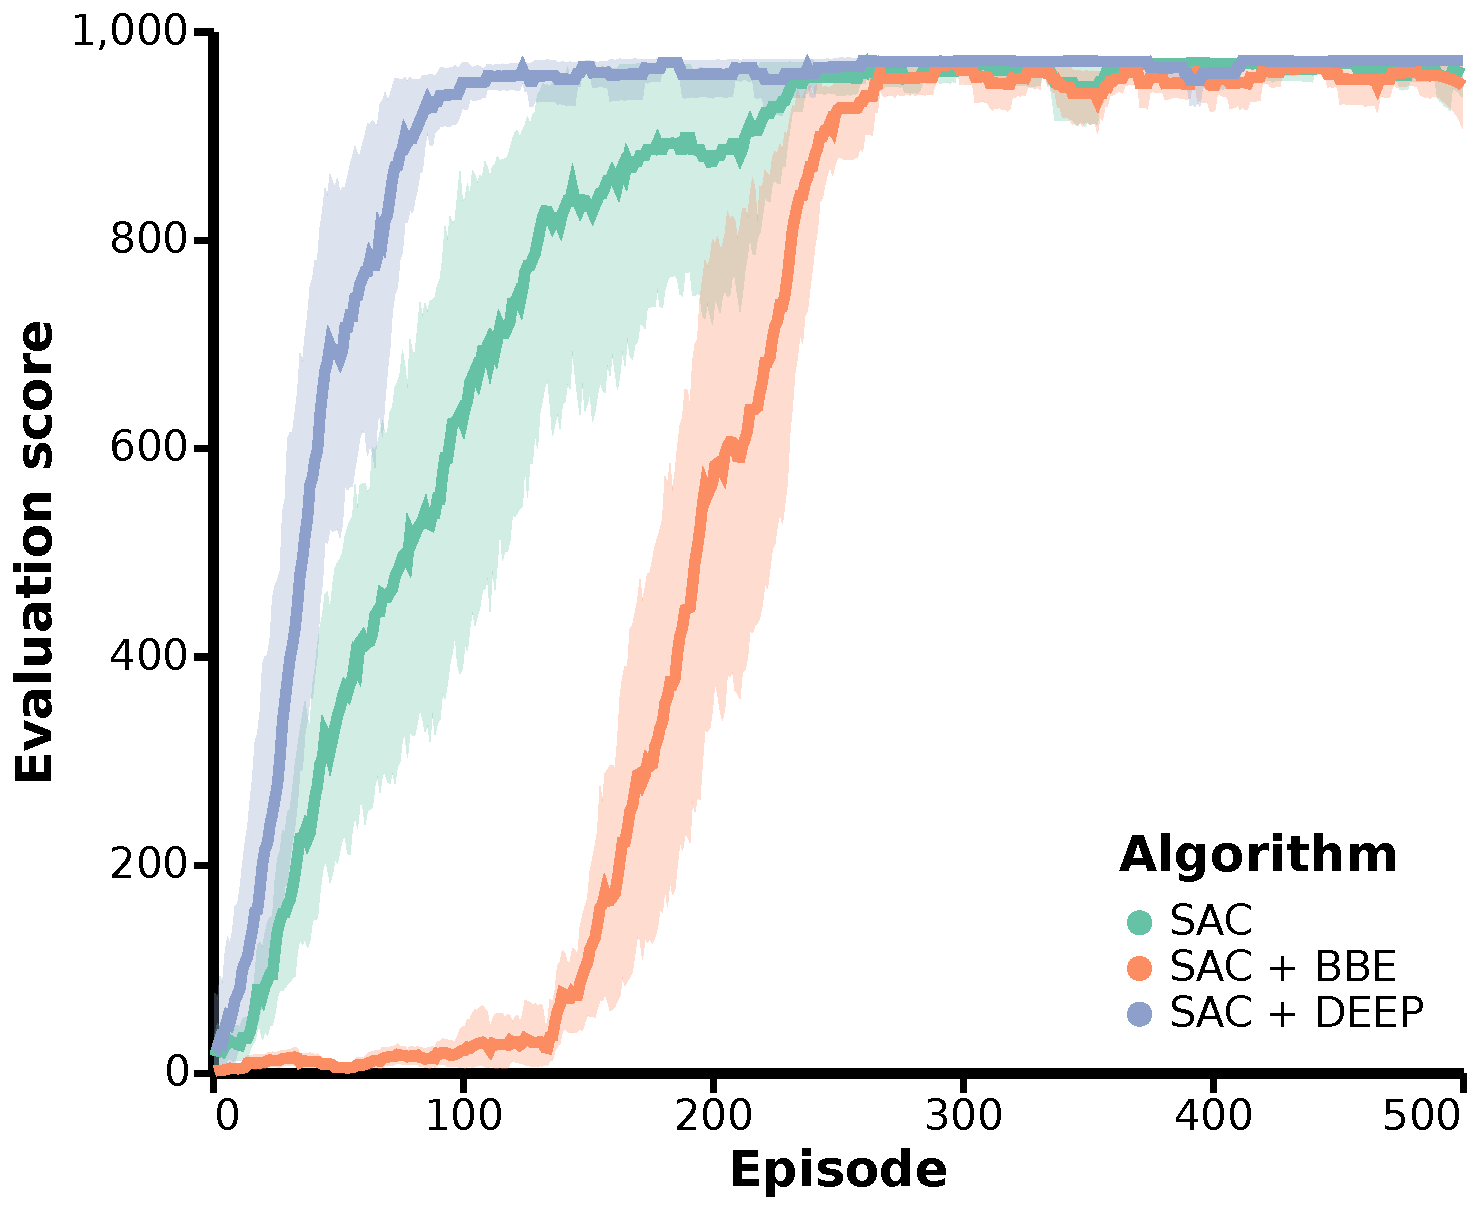
\includegraphics[width=\textwidth]{figures/deep/neurips_reacher_explore.pdf}
        \caption{Reacher explore}
    \end{subfigure}
    % \caption{Results on the original Reacher environment and on a version modified to reset the arm in one quadrant and the target in the opposite quadrant.}
    % \label{fig:reacher}
    \vspace{1em}

    \begin{subfigure}[b]{0.24\textwidth}
        \centering
        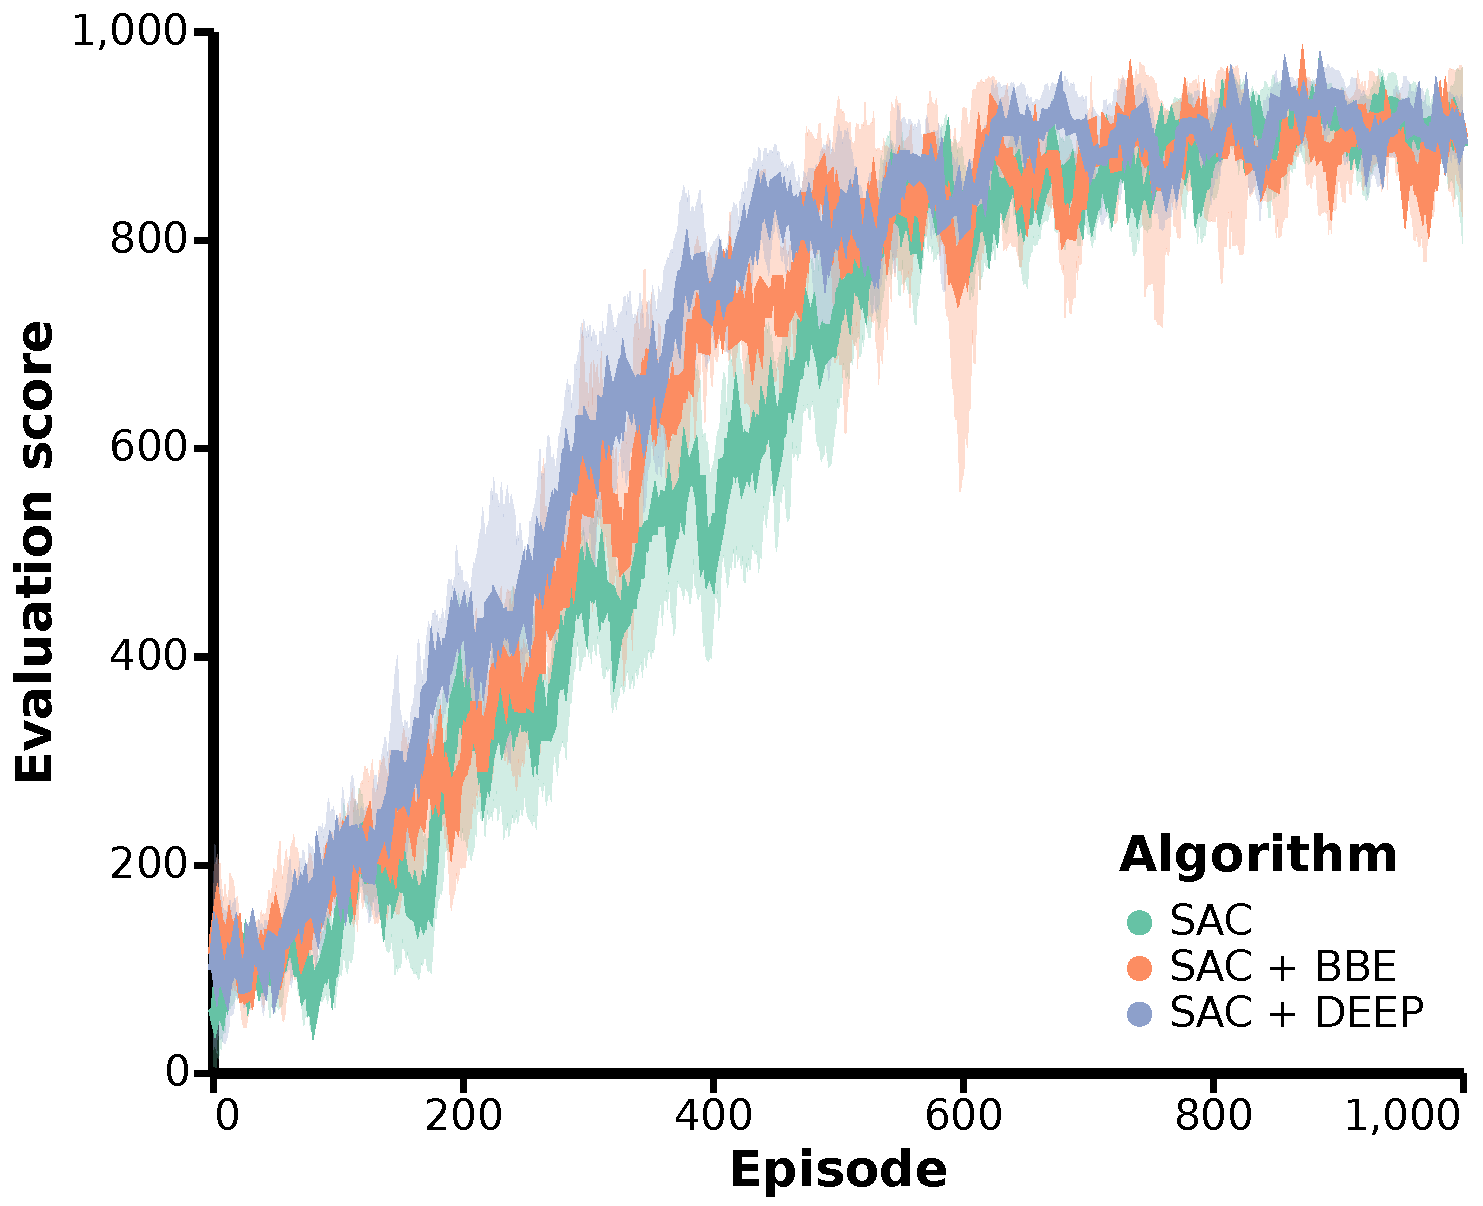
\includegraphics[width=\textwidth]{figures/deep/neurips_finger.pdf}
        \caption{Finger}
    \end{subfigure}
    \begin{subfigure}[b]{0.24\textwidth}
        \centering
        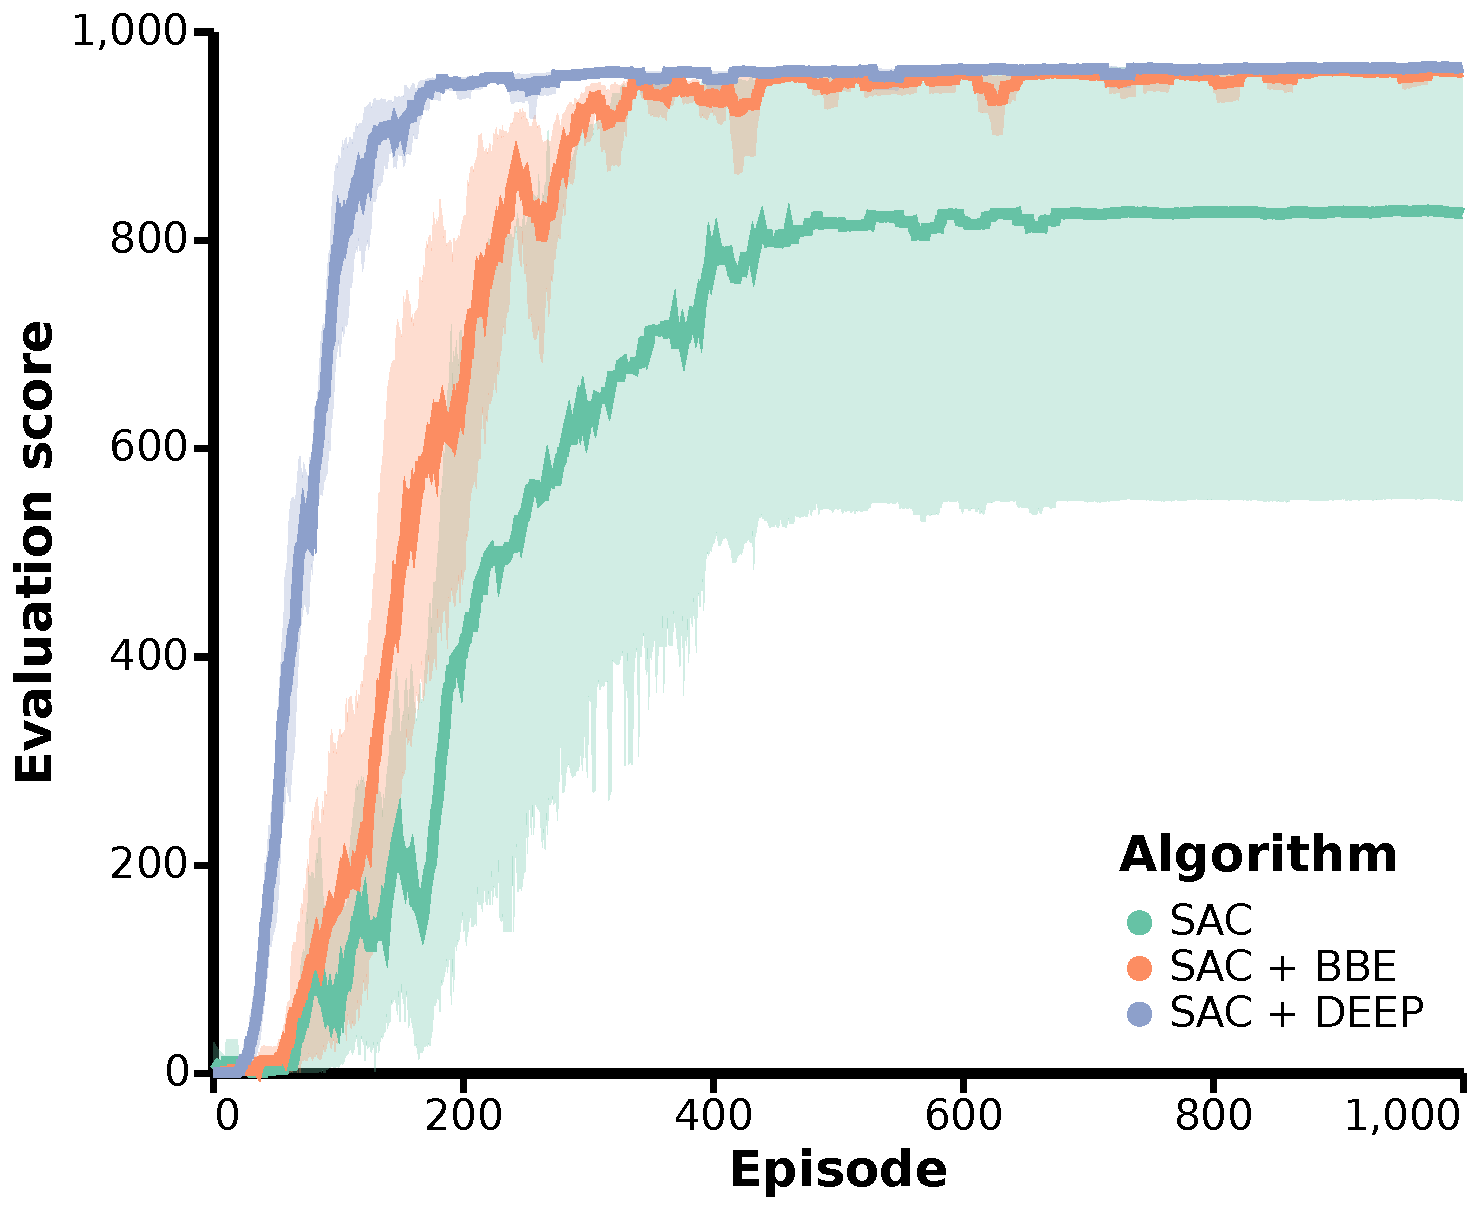
\includegraphics[width=\textwidth]{figures/deep/neurips_finger_explore.pdf}
        \caption{Finger explore}
    \end{subfigure}
    \hfill
    \begin{subfigure}[b]{0.24\textwidth}
        \centering
        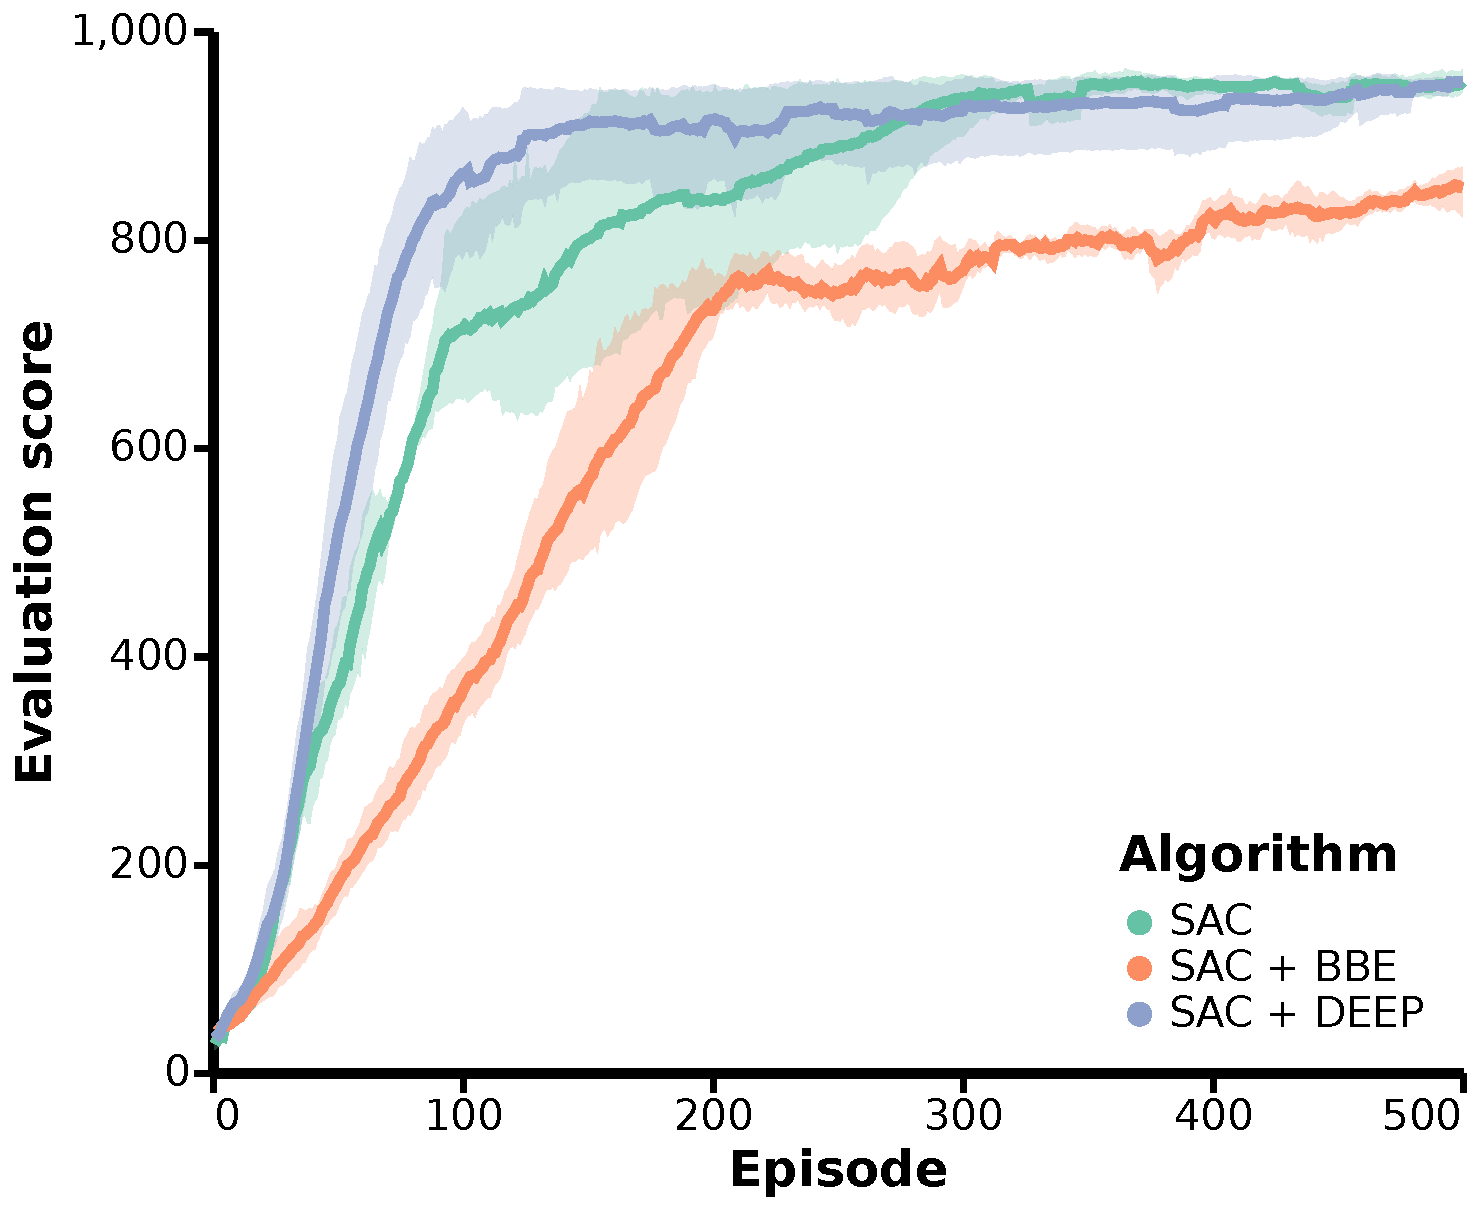
\includegraphics[width=\textwidth]{figures/deep/neurips_walker.pdf}
        \caption{Walker}
    \end{subfigure}
    \begin{subfigure}[b]{0.24\textwidth}
        \centering
        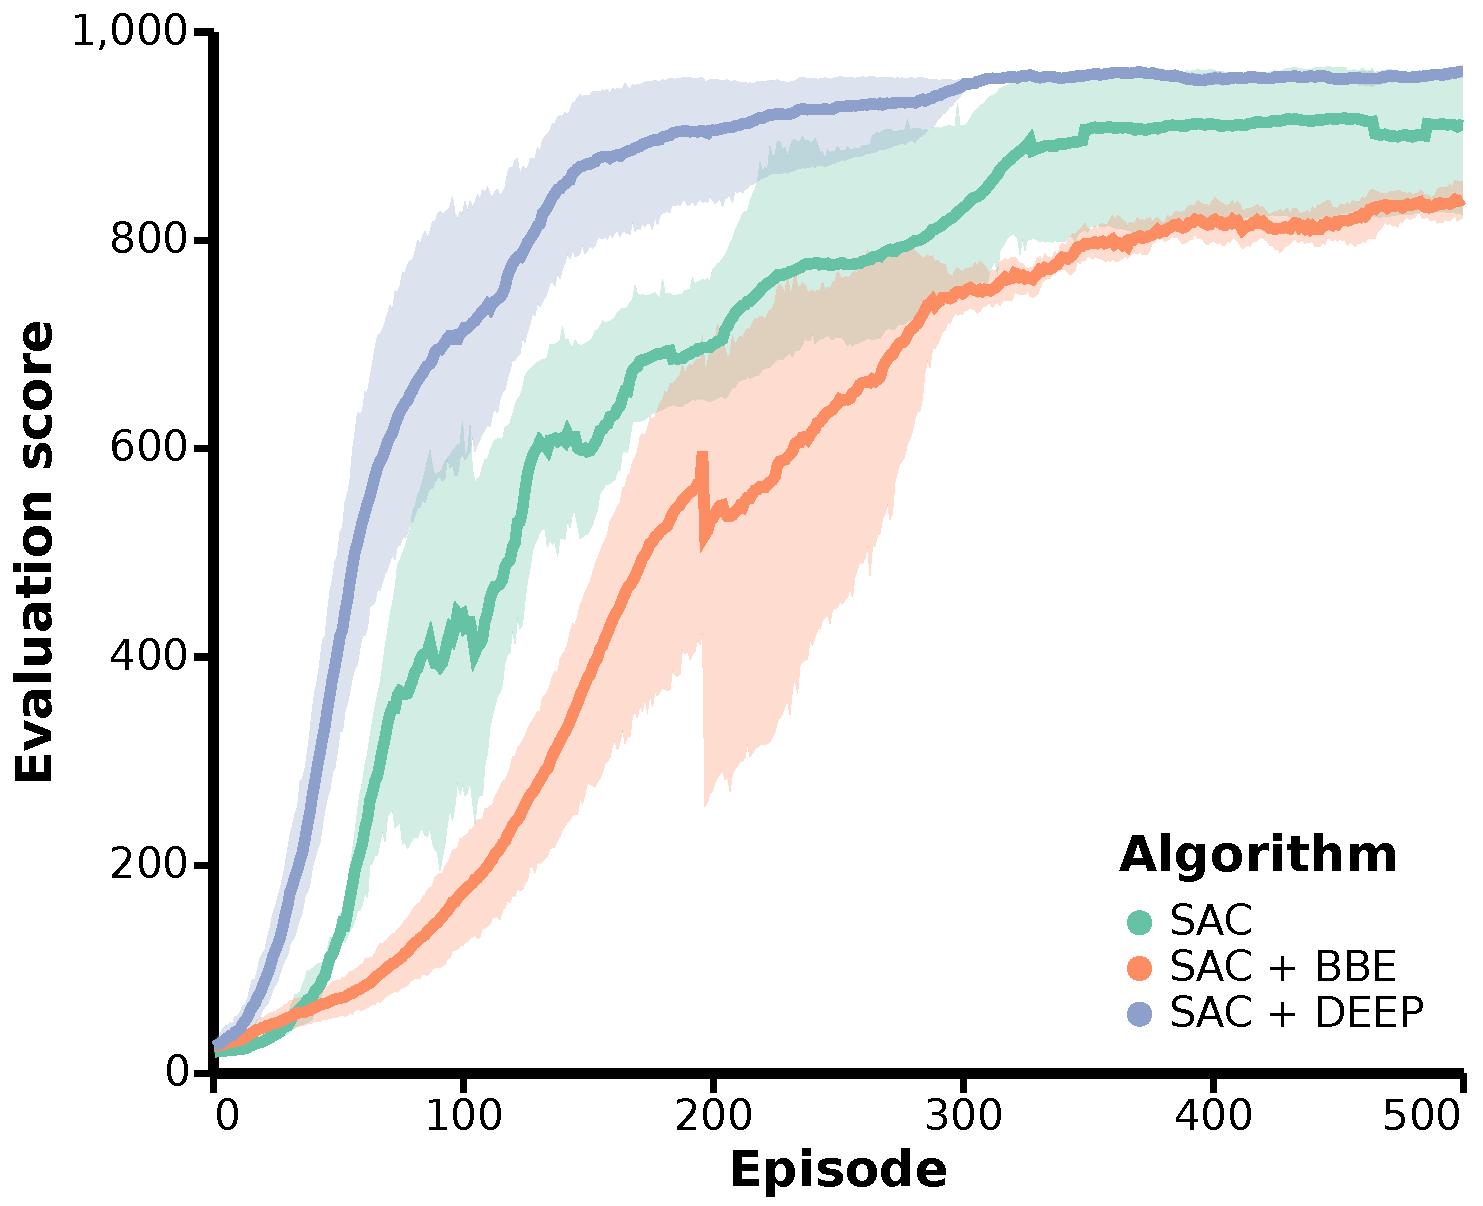
\includegraphics[width=\textwidth]{figures/deep/neurips_walker_explore.pdf}
        \caption{Walker explore}
    \end{subfigure}
    \caption{Results on original Control Suite environments (left in each pair) and modified versions without exploratory resets and rewards (right).
    Across the original environments, SAC + \algshort{} performs as well or better than SAC, while SAC + BBE performs much worse on some environments.
    On the exploration environments, \algshort{} + SAC learns much faster than SAC.
    BBE sometimes provides significant gains over SAC but sometimes performs worse even on exploration environments.
    % \red{(Rename algorithm and make fonts bigger)}}
    }
    \label{fig:control_suite}
\end{figure}

\subsubsection{Environments for evaluating exploration}
% The DeepMind Control Suite \citep{tassa2018deepmind} is a standard benchmark for continuous control RL algorithms.
While Control Suite has driven great progress in policy learning, it was not designed to evaluate an agent's exploration capabilities; in fact, the included environments were selected to be solvable by algorithms with only undirected exploration. From that work:
\begin{quote}
    We ran variety of learning agents (e.g. Lillicrap et al. 2015; Mnih et al. 2016) against all tasks, and iterated on each task’s design until we were satisfied that
    [\ldots]
    % we were satisfied that the physics was stable and non-exploitable, and that
    the task is solved correctly by at least one agent. \citep{tassa2018deepmind}
\end{quote}
Control Suite avoids the need for directed exploration via two mechanisms.
First, in many environments the start state distribution is sufficiently wide (e.g. uniform over reachable states) to guarantee that any policy will see high-value states.\endnote{Some environments, such as Manipulator, additionally start a fraction of episodes at the goal state.}
Second, some environments have rewards shaped to guide the agent towards better performance (e.g. a linearly increasing reward for forward walking speed).

To construct a benchmark for continuous control with exploration, we selected four environments with different objectives (manipulation and locomotion, single-objective or goal-conditional) and observation dimensions (6-24).
We then created ``exploration'' versions of these environments with restricted start state distributions and sparse rewards.
The original environments and their exploration versions together form a benchmark which measures an algorithm's exploration ability and policy convergence.
Environment details are in Appendix \ref{sec:environments_appendix} and their implementation is in the supplement.

\subsubsection{Algorithms}
We include experiments on these eight benchmark tasks with three algorithms: SAC \citep{haarnoja2018softapp} with no additional exploration; BBE with SAC for the policy learner; and \algshort{} with SAC for $\pitask$ and DDQN for $\piexplore$.
BBE and \algshort{} use the pseudo-count reward described in \Cref{sec:kernel_counts} and the SAC implementation is that of \citet{pytorch_sac} with no hyperparameter changes.

The kernel-based exploration bonus used for BBE and \algshort{} requires a scaling law to set the kernel variance as a function of the observation dimension.
We adapt the scaling relationship from \citep{Henderson2012NormalRB} (see Appendix \ref{sec:count_implementation}).
BBE has an additional hyperparameter for the scale of the bonus.
We performed a sweep with values in $\{ 10^{-2}, 10^{-1}, 1, 10 \}$ and found that $1$ performed best overall.
This setting, which makes the maximum bonus equal to the maximum environment reward, ensures that visiting a new state remains the best option until the true goal state is discovered.
Further implementation details are available in Appendix \ref{sec:appendix_benchmark_implementation}.
We additionally performed an ablation which, like \algshort{}, learns separate Q functions for the two rewards, but which learns one policy to maximizes the sum of their Q values.
In our experiments (available in Appendix \ref{sec:benchmark_results_appendix}) this ablation never outperforms BBE, so for clarity we exclude it here.
% Those results are available in Appendix \ref{sec:benchmark_results_appendix}.



\begin{figure}[ht]
    \centering
    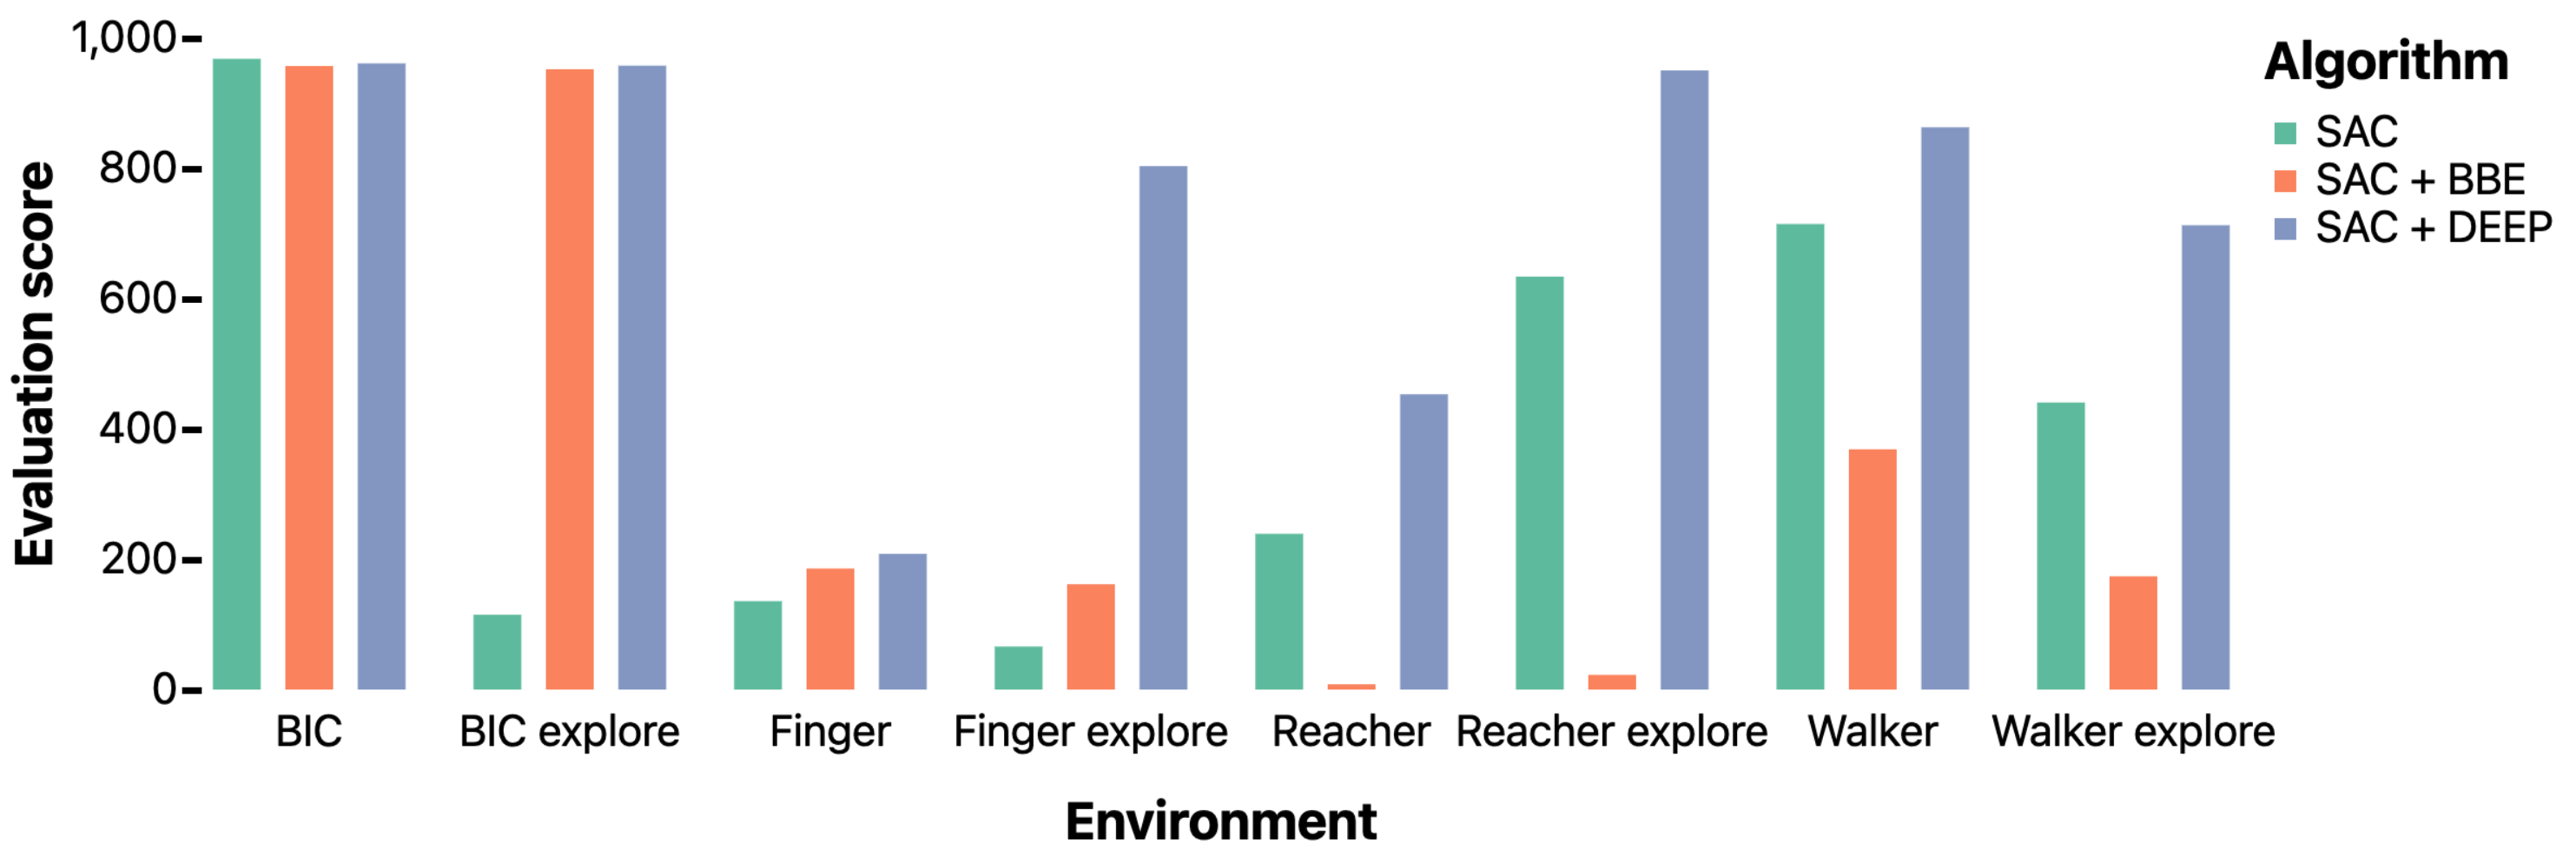
\includegraphics[width=0.95\textwidth]{figures/deep/control_suite_summary_100.png}
    \caption{Results after 100 episodes. In this extremely sample-limited regime, exploration speed and fast policy convergence are both essential. In every environment, SAC with \algshort{} (blue, right column in each set of three) performs comparably to or better than SAC alone or SAC with BBE.}
    \label{fig:control_suite_summary}
\end{figure}

We present experiments on the original versions of four Control Suite tasks and their exploration counterparts.
The results are shown in \Cref{fig:control_suite} with the means and 95\% confidence intervals over 8 seeds.
We find that across the original environments, \algshort{} gives similar or slightly better performance to SAC, while BBE significantly impairs SAC on two of the four environments and matches SAC on the other two.
Across the exploration environments, \algshort{} gives the best performance and sample efficiency.
BBE performs better than SAC alone on two exploration environments and worse than SAC on the other two.
\Cref{fig:control_suite_summary} shows the performance of each algorithm after only 100 episodes, highlighting the substantial benefits from using \algshort{} in the few-sample regime.



Overall, SAC + \algshort{} never performs worse than SAC alone, while yielding substantial improvements in environments where rewarding states are harder to discover.
BBE's more mixed performance provides a possible explanation for the limited influence that methods of that family have had on sample-efficient continuous control, and perhaps more generally on sample-efficient RL.
Given that in this setting the addition of BBE is as likely to harm as to help, its lack of adoption is unsurprising.








\section{Related work}

\paragraph{Sample-efficient continuous control.}
% As discussed in the introduction, there has been a large amount of progress on sample efficient off-policy RL that
Our method leverages progress on sample efficient off-policy RL, as it can be combined with any off-policy algorithm.
A strong line of work has brought the sample complexity of model-free control within range of solving tasks on real robots \citep{Popov2017DataefficientDR,kalashnikov2018qt,haarnoja2018soft,fujimoto2018addressing,haarnoja2018softapp,Abdolmaleki2018MaximumAP}.

% In general, current RL algorithms can be clustered into two categories: on-policy algorithms which are reliable but require hundreds of millions of environment steps to solve tasks \citep{Mnih2016AsynchronousMF,Schulman2015TrustRP,schulman2017proximal}, and recent off-policy algorithms which have brought the sample complexity of model-free control within range of solving tasks on real robots \citep{Popov2017DataefficientDR,kalashnikov2018qt,haarnoja2018softA,fujimoto2018addressing,haarnoja2018softapp,Abdolmaleki2018MaximumAP}.

%\subsection{Exploration in deep RL}

\paragraph{Bonus-based exploration.}
There have been many bonuses proposed in the BBE framework.
Several works \citep{Stadie2015IncentivizingEI,pathak2017curiosity,burda2018exploration} propose to use prediction error of a learned model to measure a transition's novelty, with the key differences being the state representation used for making predictions.
% \citet{Stadie2015IncentivizingEI} make predictions in the raw observation space, while \citet{pathak2017curiosity} use a learned embedding from an inverse dynamics model, and \citet{burda2018exploration} use a randomly-initialized neural network to embed the states.
\citet{houthooft2016vime} propose a bonus based on the information gain of the policy.
\citet{bellemare2016unifying} and others \citep{ostrovski2017count,Tang2017Exploration} use continuous count analogues to calculate the count-based bonuses of \citet{strehl2008analysis}.
%  also use the bonus formula from \citet{strehl2008analysis}, but compute counts using a locality-sensitive hashing function to bin the states.
\citet{Machado2020CountBasedEW} use the norm of learned successor features as a bonus, and show that it implicitly counts visits.
Unlike previous work, our paper focuses on the updates and representation of the behavior policy, and \algshort{} can be used in conjunction with any of these bonuses.
Never Give Up \citep{Badia2020NeverGU} uses an episodic exploration bonus and trains policies with different bonus scales including a task policy.
% exploration bonus with an episodic structure, encouraging a behavior policy to visit each state infinitely often while rapidly adapting the reward within each episode.
% Instead of a single policy, NGU learns an ensemble of policies with different scales of the exploration bonus, allowing it to act greedily with respect to a task policy.
However, it is designed to maximize asymptotic performance rather than sample efficiency and does not learn faster than a baseline early in training.


\paragraph{Optimism.}
Classic exploration methods \citep{Kearns1998NearOptimalRL,Brafman2002RMAXA,strehl2008analysis,Jaksch2008NearoptimalRB}, depend on an optimistically-defined model.
Model-free methods with theoretical guarantees \citep{Strehl2006PACMR,Jin2018IsQP} use Q functions initialized optimistically.
% Optimism is difficult to ensure with neural networks, since even an optimistic initialization will rapidly wash out due to generalization from other observed points.
Similar to our \cref{eq:optimism}, \citet{Rashid2020OptimisticEE} propose a method for ensuring optimism in Q learning with function approximation by using a count function.
% Our method uses a similar formulation for learning an optimistic exploration Q function.
However, \algshort{} leaves the task policy unbiased in the few-sample regime by separating the exploration policy from the task policy.


\paragraph{Temporally-extended actions.}
% While undirected exploration methods such as $\epsilon$-greedy explore large spaces only slowly, the use of temporally-extended actions which dither less can explore faster.
A variety of work proposes to speed up $\epsilon$-greedy exploration via temporally-extended actions which reduce dithering.
Some methods \citep{Schoknecht2003ReinforcementLO,neunert2020continuousdiscrete} propose to bias policies towards repeating primitive actions, resulting in faster exploration without limiting expressivity.
% \citet{Schoknecht2003ReinforcementLO} propose to augment the action space with multi-step actions, which consist of repeating a primitive action for a specified duration, and show that this reduces the first passage time for reaching faraway states on a random walk.
% \citet{neunert2020continuousdiscrete} propose a method for learning policies in hybrid continuous-discrete action spaces and allow the policy to choose to repeat the given action for multiple steps, resulting in faster exploration without limiting the expressivity of the policy.
\citet{Dabney2020TemporallyExtendedE} describe a temporally-extended version of $\epsilon$-greedy exploration which samples a random action and a random \emph{duration} for that action.
% They then train off-policy RL on the collected data.
\citet{Whitney2020DynamicsawareE} use a learned temporally-extended action space representing the reachable states within a fixed number of steps.
While these methods improve over single-step $\epsilon$-greedy, they are unable to perform directed exploration or discover faraway states.

% where each point in the space represents a state reachable in $k$ timesteps and a sequence of actions to get to that state, and show that uniform exploration in this space reaches faraway states with higher probability.

\paragraph{Randomized value functions.}
% Thompson sampling is a formulation of exploration that samples from the posterior distribution over value functions and then acts greedily .
Modern works \citep{Osband2016DeepEV,osband2019deep} extend Thompson sampling \citep{thompson1933likelihood} to neural networks and the full RL setting.
Relatedly, \citep{Fortunato2018NoisyNF,Plappert2018ParameterSN} learn noisy parameters and sample policies from them for exploration.


\section{Discussion}
In this paper we have investigated the potential for directed exploration to improve the sample efficiency of RL in continuous control.
We found that BBE suffers from bias and slow state coverage, leading to performance which is often worse than undirected exploration.
We introduced \algname{}, which separately learns an unbiased task policy and an exploration policy and combines them to select actions at training time.
\algshort{} pays no performance penalty even on dense-reward tasks and explores faster than BBE.
In our experiments, \algshort{} combined with SAC provides strictly better performance and sample efficiency than SAC alone.
We believe that with its combination of reliable and efficient policy learning across dense and sparse environments, SAC + \algshort{} provides a compelling default algorithm for practitioners.

\side{add appendices}

\printendnotes

\part{Representations and Auxiliary Tasks} \label{sec:representation}
Introduction to representation for RL.

\chapter{Evaluating Learned Representations} \label{sec:representation-eval}
\newcommand{\mdl}{\text{MDL}}
\newcommand{\hyp}{h}
\newcommand{\hypclass}{\mathcal{H}}
\newcommand{\method}{\textsc{LeCalf}}
\renewcommand{\eps}{\varepsilon}

\definecolor{col_a}{HTML}{FFE5E6}
\definecolor{col_b}{HTML}{E5F3FF}
\definecolor{col_c}{HTML}{E6FFE5}

\newcolumntype{a}{>{\columncolor{col_a}} r}
\newcolumntype{b}{>{\columncolor{col_b}} r}
\newcolumntype{c}{>{\columncolor{col_c}} r}

\setlength{\aboverulesep}{0pt}
\setlength{\belowrulesep}{0pt}
\setlength{\extrarowheight}{.75ex}


\section{Introduction}

One of the first steps in building a machine learning system is selecting a representation of data.
Whereas classical machine learning pipelines often begin with feature engineering, the advent of deep learning has led many to argue for pure end-to-end learning where the deep network constructs the features \citep{lecun2015deep}.
However, huge strides in unsupervised learning \citep{Hnaff2020DataEfficientIR,Chen2020ASF, he2019momentum, Oord2018RepresentationLW, bachman2019learning, devlin2018bert, liu2019roberta, raffel2019exploring, gpt3} have led to a reversal of this trend in the past two years, with common wisdom now recommending that the design of most systems start from a pretrained representation.
With this boom in representation learning techniques, practitioners and representation researchers alike have the question: Which representation is best for my task?


\begin{figure}[h]
\centering
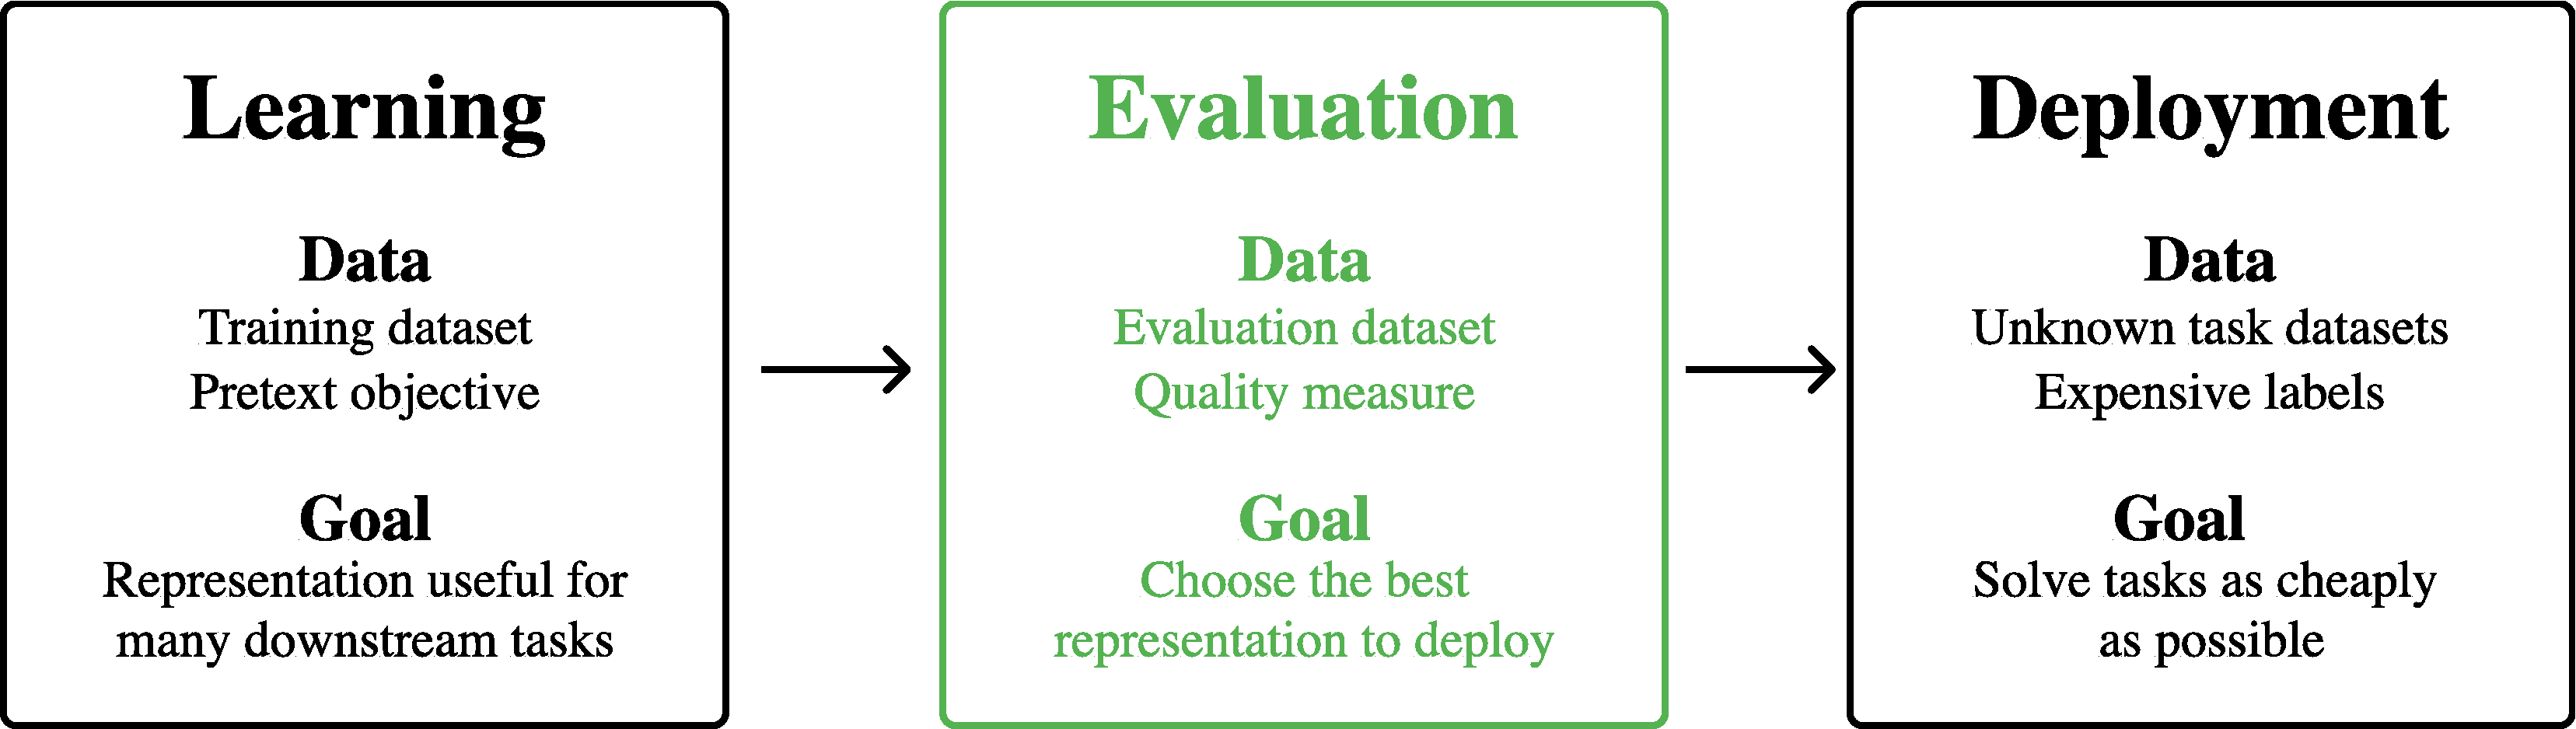
\includegraphics[width=0.48\textwidth]{figures/repr-eval/representation_pipeline.pdf}
\caption{The representation learning pipeline.}
\label{fig:representation_pipeline}
\end{figure}

This question exists as the middle step of the representation learning pipeline shown in \Cref{fig:representation_pipeline}.
The first step is representation learning, which consists of training a representation function on a training set using a pretext objective, which may be supervised or unsupervised.
The second step, which this paper considers, is representation evaluation.
In this step, one uses a measure of representation quality and a labeled \emph{evaluation dataset} to see how well the representation performs.
The final step is deployment, in which the practitioner or researcher puts the learned representation to use.
Deployment could involve using the representation on a stream of user-provided data to solve a variety of end tasks \citep{embedtheworld}, or simply releasing the trained weights of the representation function for general use.
In the same way that BERT \citep{devlin2018bert} representations have been applied to a whole host of problems, the task or amount of data available in deployment might differ from the evaluation phase.


% Answering this question in a principled manner requires deciding how to define ``task'' and ``best''.

% In this paper, we take the task to be finding a predictor that achieves low expected risk on a downstream supervised learning problem.
We take the position that the best representation is the one which allows for the most \emph{efficient} learning of a predictor to solve the task.
We will measure efficiency in terms of either number of samples or information about the optimal predictor contained in the samples.
This position is motivated by practical concerns; the more labels that are needed to solve a task in the deployment phase, the more expensive to use and the less widely applicable a representation will be.
To date the field has lacked clearly defined and motivated tools for analyzing the complexity of learning with a given representation.
This work seeks to
% elucidate the subleties of representation evaluation and
provide those tools for the representation learning community.

\begin{figure*}[t]
\begin{subfigure}[b]{.33\textwidth}
  \centering
  % include first image
  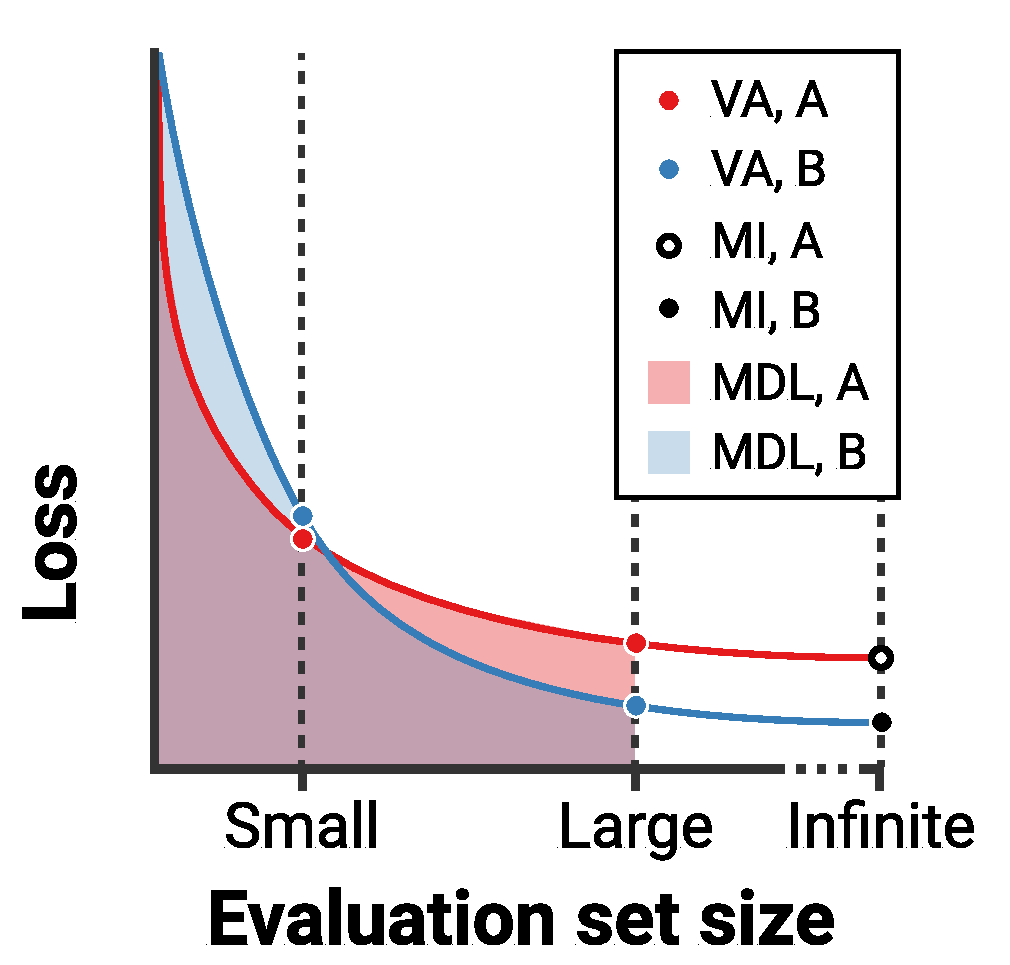
\includegraphics[height=130px]{figures/repr-eval/cartoon_left.pdf}
  \caption{Existing measures}
  \label{fig:cartoon_left}
\end{subfigure}
\begin{subfigure}[b]{.32\textwidth}
  \centering
  % include second image
  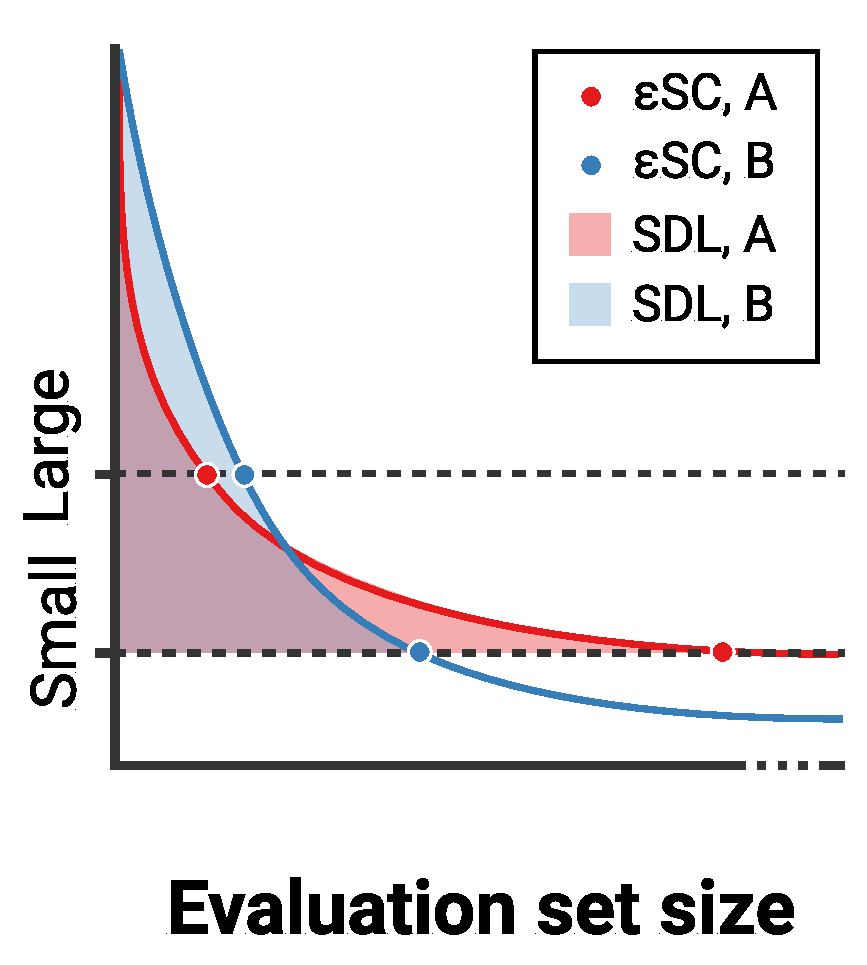
\includegraphics[height=130px]{figures/repr-eval/cartoon_right.pdf}
  \caption{Proposed measures}
  \label{fig:cartoon_right}
\end{subfigure}
\begin{subfigure}[b]{.32\textwidth}
  \centering
  % include second image
  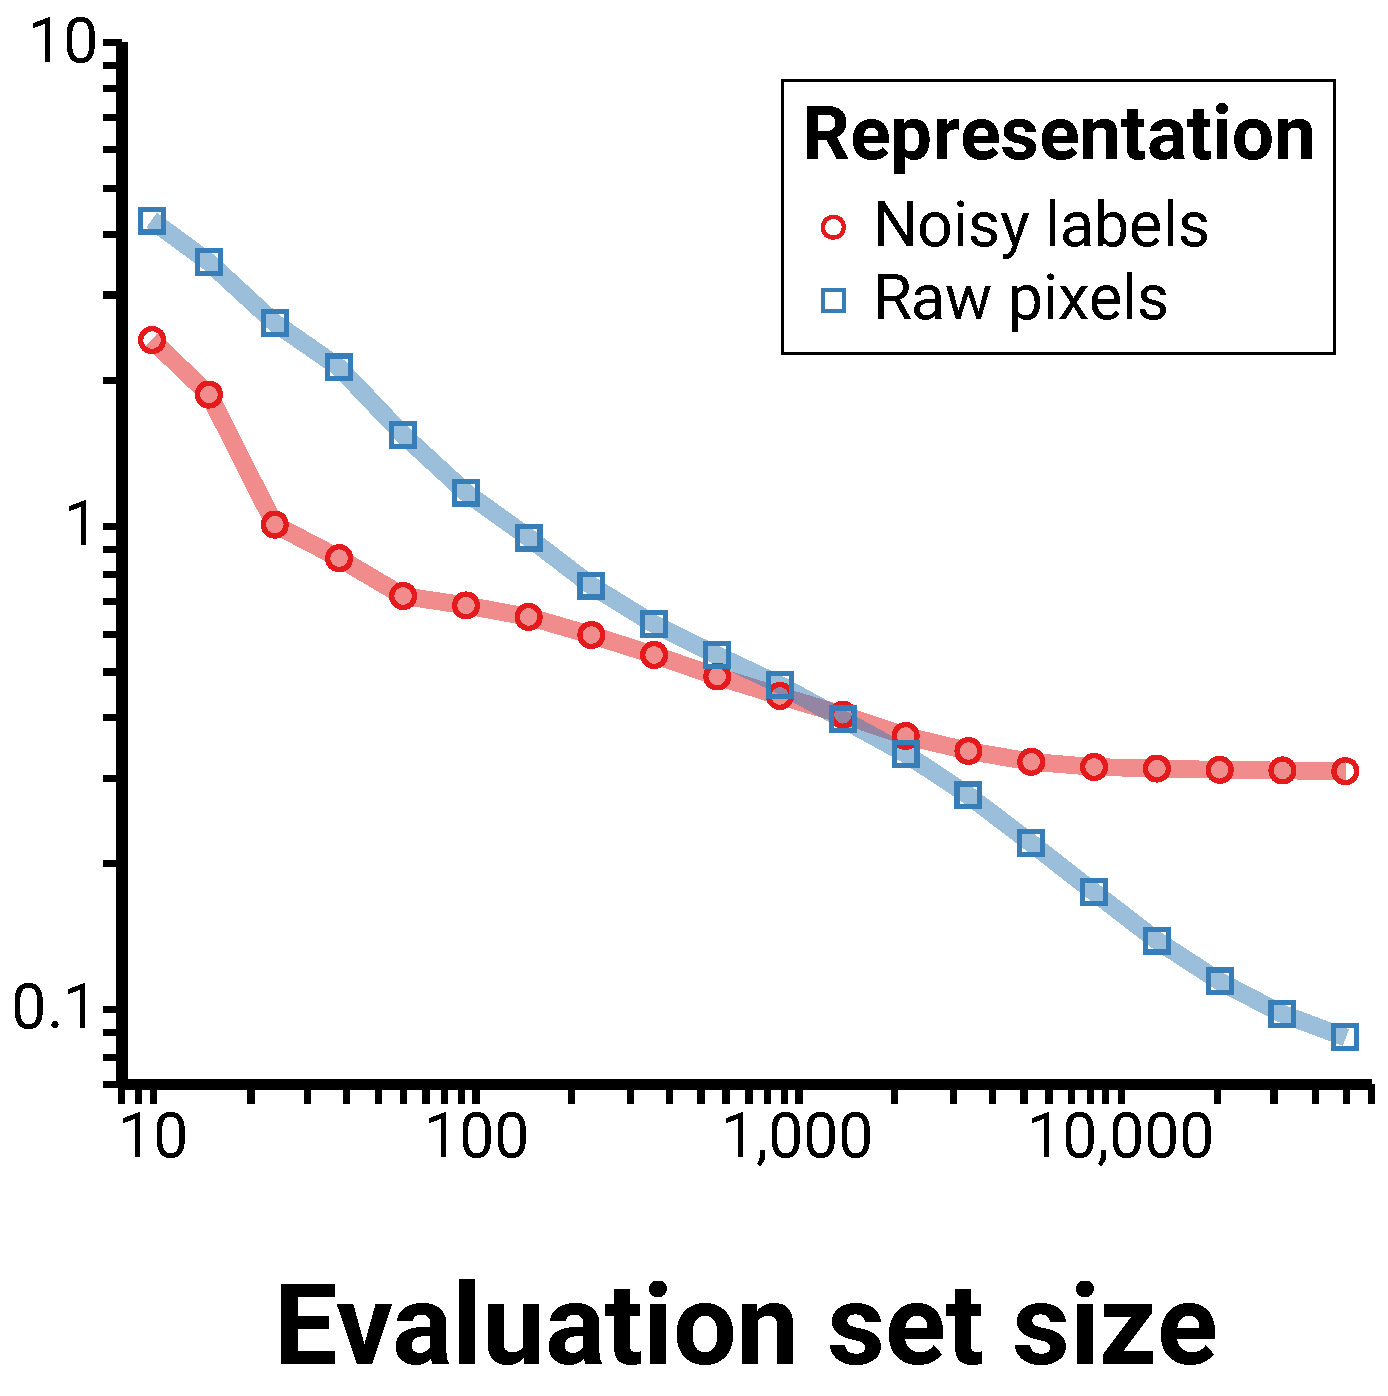
\includegraphics[height=130px]{figures/repr-eval/noisygt_bold_fixedloss.pdf}
  \caption{Illustrative experiment}
  \label{fig:noisygt}
\end{subfigure}
\caption{
Each measure for evaluating representation quality is a simple function of the ``loss-data'' curve shown here, which plots validation loss of a probe against evaluation dataset size.
\textbf{Left:} Validation accuracy (VA), mutual information (MI), and minimum description length (MDL) measure properties of a given evaluation dataset, with VA measuring the loss at a finite amount of evaluation data, MI measuring it at infinity, and MDL integrating it from zero to $n$.
This dependence on evaluation dataset size can lead to misleading conclusions as the amount of available data changes.
\textbf{Middle:} Our proposed methods instead measure the complexity of learning a predictor with a particular loss tolerance.
$ \eps$ sample complexity ($\eps$SC) measures the number of samples required to reach that loss tolerance, while surplus description length (SDL) integrates the surplus loss incurred above that tolerance.
Neither depends on the evaluation dataset size.
\textbf{Right:} A simple example task which illustrates the issue.
One representation, which consists of noisy labels, allows quick learning, while the other supports low loss in the limit of data.
Evaluating either representation at a particular evaluation dataset size risks drawing the wrong conclusion.
}
\label{fig:fig}
\end{figure*}

% This position is motivated by practical concerns; a standard ML application involves an iterative process between collecting data and learning models, and the greatest cost in many applications is data collection \red{(citation needed)}.
% The promise of representation learning is that it can enable solving new tasks while spending less effort collecting data.
% \red{MJ: The last sentence is a bit unclear to me. Alternative: we view dataset size as a quantity subject to change. This perspective is in contrast with previous evaluation methods which tend to implicitly assume that dataset size is given and fixed.}


We build on a substantial and growing body of literature that attempts to answer the question of which representation is best.
Simple, traditional means of evaluating representations, such as the validation accuracy of linear probes \citep{ettinger2016probing,Shi2016String,Alain2016Understanding}, have been widely criticized \citep{Hnaff2020DataEfficientIR,resnick2019probing}.
Instead, researchers have taken up a variety of alternatives such as the validation accuracy (VA) of nonlinear probes \citep{Conneau2018Cram,Hnaff2020DataEfficientIR}, mutual information (MI) between representations and labels \citep{bachman2019learning, Pimentel2020InformationTheoreticPF}, and minimum description length (MDL) of the labels conditioned on the representations \citep{Blier2018TheDL,Yogatama2019LinguisticIntel,Voita2020InformationTheoreticPW}.


We find that these methods all have clear limitations.
% which stem
% VA and MDL measure properties of the data, with VA measuring as the attainable accuracy using a specific amount of data and MDL measuring the compressibility of a fixed number of labels given the observations.
As can be seen in \Cref{fig:fig}, VA and MDL are liable to choose different representations for the same task when given evaluation datasets of different sizes.
Instead we want an evaluation measure which depends on the data \emph{distribution}, not a particular evaluation dataset sample or evaluation dataset size.
Furthermore, VA and MDL lack a predefined notion of success in solving a task.
In combination with small evaluation datasets, these measures may lead to premature evaluation by producing a judgement even when there is not enough data to solve the task or meaningfully distinguish one representation from another.
Meanwhile, MI measures the lowest loss achievable by any predictor irrespective of the number of samples required to learn it or the computational cost to compute it.
None of these existing techniques measure the improved data efficiency that a good representation can yield, despite this being one of the primary applications for representation learning.
% However, we note that these measures might still be appropriate for selecting representations in settings where .

% Even when none of the representations under consideration enable solving the task with the given amount of data,

% This means that a practitioner who evaluates two representations using a small dataset will choose the one
% Evaluating with a too-small dataset can lead a practitioner to make a premature choice of representation even when none have solved the task.

To eliminate these issues, we propose two measures of representation quality.
In both of our measures, the user specifies a tolerance $\eps$ so that a population loss of less than $\eps$ qualifies as solving the task.
Then the measure computes the cost of learning a predictor which achieves that loss.
% For example, a researcher might want to build representations that enable a learned model to perform at state of the art for ImageNet from pixels while using as few labels as possible, as in the contrastive representation learning work of \citet{Hnaff2020DataEfficientIR}.
% This allows them to compare the complexity of learning a specific function with  different representations.
% That is, the user specifies a target function and these measures compute how complex it is to learn.
% i.e. approximating the optimal predictor to low error.
The first measure is the \emph{surplus description length} (SDL) which modifies the MDL to measure the complexity of learning an $\eps$-loss predictor rather than computing the complexity of the labels in the evaluation dataset.
The second is the \emph{$\eps$-sample complexity} ($\eps$SC) which measures the sample complexity of learning an $\eps$-loss predictor.
These measures resolve the issues with prior work and provide tools for researchers and practitioners to evaluate the extent to which a learned representation can improve data efficiency.
Furthermore, they formalize existing research challenges for learning representations which allow state of the art performance while using as few labels as possible (e.g.~\citet{Hnaff2020DataEfficientIR}).

To facilitate our analysis, we also propose a framework called the \emph{loss-data framework}, illustrated in \Cref{fig:fig}, that plots the validation loss against the evaluation dataset size \citep{Talmor2019oLMpics, Yogatama2019LinguisticIntel, Voita2020InformationTheoreticPW}.
This framework simplifies comparisons between measures.
Prior work measures integrals (MDL) and slices (VA and MI) along the data axis.
Our work proposes instead measuring integrals (SDL) and slices ($\eps$SC) along the loss axis.
This illustrates how prior work makes tacit choices about the function to learn based on the choice of evaluation dataset size.
Our work instead makes an explicit, interpretable choice of what function to learn via the threshold $\eps$ and measures the complexity of learning such a function.
We experimentally investigate the behavior of these methods, illustrating the sensitivity of VA and MDL, and the robustness of SDL and $\eps$SC, to evaluation dataset size.

\paragraph{Efficient implementation.} To enable reproducible representation evaluation for representation researchers, we have developed a highly optimized open source Python package
at \url{https://github.com/willwhitney/reprieve}.
This package enables construction of loss-data curves with arbitrary representations and datasets and is library-agnostic, supporting representations and learning algorithms implemented in any Python ML library.
By leveraging the JAX library \citep{jax2018github} to parallelize the training of probes on a single accelerator, our package constructs loss-data curves in around two minutes on one GPU.



\section{The loss-data framework for representation evaluation}

In this section we formally present the representation evaluation problem, define our loss-data framework, and show how prior work fits into the framework.


\paragraph{Notation.}
We use bold letters to denote random variables.
A supervised learning problem is defined by a joint distribution $ \mathcal{D}$ over
observations and labels $(\rmX, \rmY)$ in the sample space $ \mathcal{X} \times \mathcal{Y}$ with density denoted by $ p$.
Let the random variable $\rmD^n$ be a sample of $n$ i.i.d. $(\rmX, \rmY)$ pairs, realized by $D^n = (X^n, Y^n) = \{(x_i, y_i)\}_{i=1}^n$.
This is the evaluation dataset.
Let $ \mathcal{R}$ denote a representation space and $\phi: \mathcal{X} \to \mathcal{R}$ a representation function.
The methods we consider all use parametric probes, which are neural networks $\hat{p}_\theta: \mathcal{R} \to P(\mathcal{Y})$ parameterized by $ \theta\in \R^d$ that are trained on $D^n$ to estimate the conditional distribution $p(y \mid x)$.
We often abstract away the details of learning the probe by simply referring to an algorithm $\mathcal{A}$ which returns a predictor: $\hat{p} = \mathcal{A}(\phi(D^n))$. Abusing notation, we denote the composition of $ \mathcal{A}$ with $\phi$ by $\mathcal{A}_\phi$.
Define the population loss and the expected population loss for $\hat{p} = \mathcal{A}_\phi(D^n)$, respectively as
\begin{align}
    L(\mathcal{A}_\phi, D^n) = \E_{(\rmX, \rmY)} - \log \hat{p}(\rmY \mid \rmX) \label{eq:loss_data} && L(\mathcal{A}_\phi, n) = \E_{\rmD^n} L(\mathcal{A}_\phi, \rmD^n). %\label{eq:loss_n}
\end{align}
The expected population loss averages over evaluation dataset samples, removing the variance that comes from using some particular evaluation dataset to train a probe.
In this section we will focus on population quantities, but note that any algorithmic implementation must replace these by their empirical counterparts.

\paragraph{The representation evaluation problem.} The representation evaluation problem asks us to define a real-valued measurement of the quality of a representation $ \phi$ for solving solving the task defined by $(\rmX, \rmY)$. Explicitly, each method defines a real-valued function $ m(\phi, \mathcal{D}, \mathcal{A}, \Psi)$ of a representation $\phi$, data distribution $ \mathcal{D}$, probing algorithm $ \mathcal{A}$, and some method-specific set of hyperparameters $ \Psi $. By convention, smaller values of the measure $ m $ correspond to better representations.
Defining such a measurement allows us to compare different representations.



\subsection{Defining the loss-data framework.}
The loss-data framework is a lens through which we contrast different measures  of representation quality. The key idea, demonstrated in \Cref{fig:fig}, is to plot the loss $ L(\mathcal{A}_\phi, n) $ against the evaluation dataset size $ n$.
Explicitly, at each $ n$, we train a probing algorithm $ \mathcal{A}$ using a representation $ \phi$ to produce a predictor $ \hat p$, and then plot the loss of $ \hat p$ against $ n$.
Similar analysis has appeared in \citet{Voita2020InformationTheoreticPW, Yogatama2019LinguisticIntel, Talmor2019oLMpics}.
We can represent each of the prior measures as points on the curve at fixed $ x $ (VA, MI) or integrals of the curve along the $ x$-axis (MDL).
Our measures correspond to evaluating points at fixed $ y $ ($\eps$SC) and integrals along the $ y$-axis (SDL).


\subsection{Existing methods in the loss-data framework} \label{sec:existing_methods}

\paragraph{Nonlinear probes with limited data.}

A simple strategy for evaluating representations is to choose a probe architecture and train it on a limited amount of data from the task and representation of interest \citep{Hnaff2020DataEfficientIR, Zhang2018LanguageMT}.
Each representation is typically scored by its validation accuracy, leading us to call this the validation accuracy (VA) measure.
This method can be interpreted in our framework by replacing the validation accuracy with the validation loss and taking an expectation over draws of evaluation datasets of size $n$.
On the loss-data curve, this measure corresponds to evaluation at $x=n$, so that
\begin{align}
    m_{\mathrm{VA}}(\phi, \mathcal{D}, \mathcal{A}, n) = L(\mathcal{A}_\phi, n).
\end{align}

\paragraph{Mutual information.}
Mutual information (MI) between a representation $\phi(\rmX)$ and targets $\rmY$ is another often-proposed metric for learning and evaluating representations \citep{Pimentel2020InformationTheoreticPF, bachman2019learning}.
In terms of entropy, mutual information is equivalent to the information gain about $\rmY$ from knowing $\phi(\rmX)$:
\begin{align}
    I(\phi(\rmX); \rmY) = H(\rmY) - H(\rmY \mid \phi(\rmX)).
\end{align}
In general mutual information is intractable to estimate for high-dimensional or continuous-valued variables \citep{McAllester2018FormalLO}, and a common approach is to use a very expressive model for $\hat{p}$ and maximize a variational lower bound:
\begin{align}
    I(\phi(\rmX); \rmY) &\ge H(\rmY) + \E_{(\rmX, \rmY)} \log \hat{p}(\rmY \mid \phi(\rmX)).
\end{align}
Since $H(\rmY)$ is not a function of the parameters, maximizing the lower bound is equivalent to minimizing the negative log-likelihood.
Moreover, if we assume that $ \hat p$ is expressive enough to represent $ p$ and take $ n \to \infty$, this inequality becomes tight.
As such, MI estimation can be seen a special case of nonlinear probes as described above, where instead of choosing some particular setting of $n$ we push it to infinity. We formally define the mutual information measure of a representation as
\begin{align}
    m_{\mathrm{MI}}(\phi, \mathcal{D}, \mathcal{A}) = \lim_{n\to \infty} L(\mathcal{A}_\phi, n).
\end{align}
A decrease in this measure reflects an increase in the mutual information.
On the loss-data curve, this corresponds to evaluation at $ x= \infty$.


\paragraph{Minimum description length.}
Recent studies \citep{Yogatama2019LinguisticIntel,Voita2020InformationTheoreticPW} propose using the Minimum Description Length (MDL) principle \citep{Rissanen1978ModelingBS,Grnwald2004ATI} to evaluate representations.
These works use an online or prequential code \citep{Blier2018TheDL} to encode the labels given the representations. The codelength $ \ell$ of $ Y^n $ given $ \phi(X^n) $ is then defined as
\begin{align}
    \ell(Y^n \mid \phi(X^n)) = - \sum_{i=1}^n \log \hat{p}_i(y_{i} \mid \phi(x_{i})),
\end{align}
where $\hat{p}_i$ is the output of running a pre-specified algorithm $\mathcal{A}$ on the evaluation dataset up to element $i$: $\hat{p}_i = \mathcal{A}_\phi(X^n_{1:i}, Y^n_{1:i})$.
This measure can exhibit large variance on small evaluation datasets, especially since it is sensitive to the (random) order in which the examples are presented.
We remove this variance by taking an expectation over the sampled evaluation datasets for each $i$ and define a population variant of the MDL measure~\citep{Voita2020InformationTheoreticPW} as
\begin{align} \label{eq:mdl_expected}
    m_{\mathrm{MDL}}(\phi, \mathcal{D}, \mathcal{A},n) = \E \Big[ \ell(\rmY^n \mid \phi(\rmX^n)) \Big] = \sum_{i=1}^n L(\mathcal{A}, i).
\end{align}
Thus, $m_\mathrm{MDL}$ measures the area under the loss-data curve on the interval $x \in [0, n]$.

\section{Limitations of existing methods}

Each of the prior methods, VA, MDL, and MI, have limitations that we attempt to solve with our methods. In this section we present these limitations.

\subsection{Sensitivity to evaluation set size in VA and MDL}
As seen in \Cref{sec:existing_methods}, the representation quality measures of VA and MDL
both depend on $n$, the size of the evaluation dataset.
Because of this dependence, the ranking of representations given by these evaluation metrics can change as $n$ increases.
Choosing to deploy one representation rather than another by comparing these metrics at arbitrary $n$ may lead to premature decisions in the machine learning pipeline since a larger  evaluation dataset could give a different ordering.


\paragraph{A theoretical example.}
\label{sec:counter_ex}
Let $s \in \{0,1\}^d$ be a fixed binary vector and consider a data generation process where the $\{0,1\}$ label of a data point is given by the parity on $s$, i.e., $y_i = \langle x_i, s \rangle \bmod{2}$ where $y_i \in \{0,1\}$ and $x_i \in \{0,1\}^d$. Let $Y^n = \{y_i\}_{i=1}^n$ be the given labels and consider the following two representations: (1) Noisy label: $z_i = \langle x_i, s \rangle + e_i \bmod{2}$, where $e_i \in \{0,1\}$ is a random bit with bias $\alpha < 1/2$, and (2) Raw data: $x_i$.

For the noisy label representation, guessing $y_i = z_i$ achieves validation accuracy of $1-\alpha$ for any $n$, which, is information-theoretically optimal. On the other hand, the raw data representation will achieve perfect validation accuracy once the evaluation dataset contains $d$ linearly independent $x_i$'s. In this case, Gaussian elimination will exactly recover $s$. The probability that a set of $n > d$ random vectors in $\{0,1\}^d$ does not contain $d$ linearly independent vectors decreases exponentially in $n-d$. Hence, the expected validation accuracy for $n$ sufficiently larger than $d$ will be exponentially close to 1. As a result, the representation ranking given by validation accuracy and description length favors the noisy label representation when $n \ll d$, but the raw data representation will be much better in these metrics when $n \gg d$. This can be misleading.
Although this is a concocted example for illustration purposes, our experiments in \Cref{sec:experiments} validate that dependence of representation rankings on $n$ does occur in practice.

\subsection{Insensitivity to representation quality  \& computational complexity in MI}
\label{sec:mutual_info}
MI considers the lowest validation loss achievable with the given representation and ignores any concerns about statistical or computational complexity of achieving such accuracy.
This leads to some counterintuitive properties which make MI an undesirable metric:
\begin{enumerate}
    \item MI is insensitive to statistical complexity. Two random variables which are perfectly predictive of one another have maximal MI, though their relationship may be sufficiently complex that it requires exponentially many samples to verify~\citep{McAllester2018FormalLO}.
    \item MI is insensitive to computational complexity. For example, the mutual information between an intercepted encrypted message and the enemy's plan is high~\citep{Shannon1948TheMT, Xu2020ATheory}, despite the extreme computational cost required to break the encryption.
    \item MI is insensitive to representation. By the data processing inequality \citep{Cover2006ElementsOI}, \emph{any} $\phi$ applied to $\rmX$ can only decrease its mutual information with $\rmY$; no matter the query, MI always reports that the raw data is at least as good as the best representation.
\end{enumerate}


\subsection{Lack of a predefined notion of success}
All three prior methods lack a predefined notion of successfully solving a task and
will always return some ordering of representations.
When the evaluation dataset is too small or all of the representations are poor, it may be that no representation can yet solve the task (i.e. achieve a useful accuracy).
Since the order of representations can change as more data is added, any judgement would be premature.
Indeed, there is often an implicit minimum requirement for the loss a representation should achieve to be considered meaningful.
As we show in the next section, our methods makes this requirement explicit.



\section{Surplus description length \& $\eps$ sample complexity}

The methods discussed above measure a property of the data, such as the attainable accuracy on $n$ points, by learning an unspecified function.
Instead, we propose to precisely define the function of interest and measure its complexity using data.
Fundamentally, we shift from making a statement about the inputs of an algorithm, like VA and MDL do, to a statement about the outputs.

\subsection{Surplus description length (SDL)}
Imagine trying to efficiently encode a large number of samples of a random variable $\rve$ which takes values in $\{1 \ldots K\}$ with probability $p(\rve)$.
An optimal code for these events has expected length\endnote{Code length in nats due to the base $e$.} $\E[\ell(\rve)] = \E_{\rve} [ - \log p(\rve)] = H(\rve)$.
If this data is instead encoded using a probability distribution $\hat p$, the expected length becomes $H(\rve) + \KL{p}{\hat p}$.
We call $\KL{p}{\hat p}$ the \emph{surplus description length} (SDL) from encoding according to $\hat p$ instead of $p$:
\begin{align}
    \KL{p}{\hat p}
    = \E_{\rve \sim p} \left[ \log p(\rve) - \log \hat p(\rve) \right].
\end{align}
When the true distribution $p$ is a delta, the entire length of a code under $\hat p$ is surplus since $\log 1 = 0$.

Recall that the prequential code for estimating MDL computes the description length of the labels given observations in an evaluation dataset by iteratively creating tighter approximations $\hat p_{1} \ldots \hat p_{n}$ and integrating the area under the curve.
Examining \Cref{eq:mdl_expected}, we see that
\begin{align}
     m_{\mathrm{MDL}}(\phi, \mathcal{D}, \mathcal{A},n) = \sum_{i=1}^n L(\mathcal{A}_\phi, i) \geq \sum_{i=1}^n H(\rmY \mid \phi(\rmX)).
\end{align}

If $H(\rmY \mid \phi(\rmX)) > 0$, MDL grows without bound as the size of the evaluation dataset $n$ increases.

Instead, we propose to measure the complexity of a learned predictor $p(\rmY \mid \phi(\rmX))$ by computing the surplus description length of encoding an infinite stream of data according to the online code instead of the true conditional distribution.
\begin{definition}[Surplus description length of online codes] \label{def:sdl_entropy}
    Given random variables $\rmX, \rmY \sim \mathcal{D}$, a representation function $ \phi$, and a learning algorithm $\mathcal{A}$, define
    \begin{align}
        m_{\mathrm{SDL}}(\phi, \mathcal{D}, \mathcal{A}) &=
        \sum_{i=1}^\infty \Big[ L(\mathcal{A}_\phi, i) - H(\rmY \mid \rmX) \Big].
    \end{align}
\end{definition}
This surplus description length beyond the optimal code improves on MDL by being bounded.
However, as discussed in \Cref{sec:mutual_info} entropy is intractible to estimate, and in practice it is more relevant to measure the cost of learning a good enough predictor rather than a theoretically perfect one.

We generalize this definition to measure the complexity of learning an approximating conditional distribution with loss $\eps$.
This corresponds to the additional description length incurred by encoding data with the learning algorithm $\mathcal{A}$ rather than using a fixed predictor with loss $\eps$.
\begin{definition}[Surplus description length of online codes with a specified baseline] \label{def:sdl}
    Take random variables $\rmX, \rmY \sim \mathcal{D}$, a representation function $ \phi$, a learning algorithm $\mathcal{A}$, and a loss tolerance $\eps \ge H(\rmY \mid \rmX)$. Let $[c]_+$ denote $\max(0, c)$ and then we define
    \begin{align}
        m_{\mathrm{SDL}}(\phi, \mathcal{D}, \mathcal{A},\eps) &= \sum_{i=1}^\infty \Big[ L(\mathcal{A}_\phi, i) - \eps \Big]_+.
    \end{align}
\end{definition}
One interpretation of this measure is that it gives the cost (in terms of information) for re-creating an $\eps$-loss predictor when using the representation $\phi$.

In our framework, the surplus description length corresponds to computing the area between the loss-data curve and a baseline set by $y = \eps$.
Whereas MDL measures the complexity of a sample of $n$ points, SDL measures the complexity of a function which solves the task to $\eps$ tolerance.

\paragraph{Estimating the SDL.}
Naively computing SDL would require unbounded data and the estimation of $L(\mathcal{A}_\phi, i)$ for every $i$.
However, any reasonable learning algorithm obtains a better-generalizing predictor when given more i.i.d. data from the target distribution \citep{Kaplan2020ScalingLF}.
If we assume that algorithms are monotonically improving so that $L(\mathcal{A}, i+1) \le L(\mathcal{A}, i)$, SDL only depends on $i$ up to the first point where $L(\mathcal{A}, n) \le \eps$.
Approximating this integral can be done efficiently by taking a log-uniform partition of the evaluation dataset size and computing the Riemann sum as in \citet{Voita2020InformationTheoreticPW}.
Note that evaluating a representation only requires training probes, not the large representation functions themselves, and thus has modest computational requirements.
Crucially, if the tolerance $\eps$ is set unrealizeably low or the amount of available data is insufficient, an implementation is able to report that the given complexity estimate is only a lower bound.


\subsection{$\eps$ sample complexity ($\eps$SC)}

In addition to surplus description length we introduce a second, conceptually simpler measure of representation quality: $\eps$ sample complexity.

\begin{definition}[Sample complexity of an $\eps$-loss predictor] \label{def:sample_complexity}
    Given random variables $\rmX, \rmY \sim \mathcal{D}$, a representation function $ \phi$, a learning algorithm $\mathcal{A}$, and a loss tolerance $\eps \ge H(\rmY \mid \phi(\rmX))$, define
    \begin{align}
         m_{\eps\mathrm{SC}}(\phi, \mathcal{D}, \mathcal{A},\eps) &= \min \Big\{ n \in \mathbb{N} : L(\mathcal{A}_\phi, n) \leq \eps \Big\}.
    \end{align}
\end{definition}

The $\eps$ sample complexity measures the complexity of learning an $\eps$-loss predictor by the number of samples it takes
to find it.
This measure allows the comparison of two representations by first picking a target function to learn (via a setting of $\eps$), then measuring which representation enables learning that function with less data.

In our framework, sample complexity corresponds to taking a horizontal slice of the loss-data curve at $y = \eps$, analogous to VA's slice at $y=n$.
VA makes a statement about the data (by setting $n$) and reports the accuracy of some function given that data.
In contrast, $\eps$ sample complexity specifies the desired function and determines its complexity by how many samples are needed to learn it.

\paragraph{Estimating the $\eps$SC.}
Given an assumption that algorithms are monotonically improving such that $ L(\mathcal{A}, n+1) \le L(\mathcal{A}, n)$, $\eps$SC can be estimated efficiently.
With $n$ finite samples in the evaluation dataset, an algorithm may estimate $\eps$SC by splitting the data into $k$ uniform-sized bins and estimating $L(\mathcal{A}, \nicefrac{ik}{n})$ for $i \in \{1 \ldots k \}$.
By recursively performing this search on the interval which contains the transition from $L > \eps$ to $L < \eps$, we can rapidly reach a precise estimate or report that $m_{\eps\mathrm{SC}}(\phi, \mathcal{D}, \mathcal{A},\eps) > n$.

\paragraph{Using objectives other than negative log-likelihood.}
% \todo{this}
Our exposition of $\eps$SC uses negative log-likelihood for consistency with other methods, such as MDL, which require it.
However, it is straightforward to extend $\eps$SC to work with whatever objective function is desired under the assumption that said objective is monotone with increasing data when using algorithm $\mathcal{A}$.
A natural choice in many cases would be prediction accuracy, where a practitioner might target e.g. a 95\% accurate predictor.

\subsection{Setting $\eps$}

A value for the threshold $\eps$ corresponds to the set of $\eps$-loss predictors that a representation should make easy to learn.
Choices of $\eps \ge H(\rmY \mid \rmX)$ represent attainable functions, while selecting $\eps < H(\rmY \mid \rmX)$ leads to unbounded SDL and $\eps$SC for any choice of the algorithm $\mathcal{A}$.

For evaluating representation learning methods in the research community, we recommend using SDL and establishing benchmarks which specify (1) a downstream task, in the form of an evaluation dataset; (2) a criterion for success, in the form of a setting of $\eps$; (3) a standard probing algorithm $\mathcal{A}$.
The setting of $\eps$ can be done by training a large model on the raw representation of the full evaluation dataset and using its validation loss as $\eps$ when evaluating other representations.
This guarantees that $\eps \ge H(\rmY \mid \rmX)$ and the task is feasible with any representation at least as good as the raw data.
In turn, this ensures that SDL is bounded.


In practical applications, $\eps$ should be a part of the design specification for a system.
As an example, a practitioner might know that an object detection system with 80\% per-frame accuracy is sufficient and labels are expensive.
For this task, the best representation would be one which enables the most sample efficient learning of a predictor with error $\eps = 0.2$ using a 0~--~1 loss.





\section{Experiments} \label{sec:experiments}

We empirically show the behavior of VA, MDL, SDL, and $\eps$SC with two sets of experiments on real data.
These experiments have the following goals:
\begin{enumerate}
    \item Test whether the theoretical issue of sensitivity to evaluation dataset size for VA and MDL occurs in practice.
    \item Demonstrate that SDL and $\eps$SC produce lower bounds when insufficient data is available and concrete quantities otherwise.
    \item Evaluate whether the computation of SDL and $\eps$SC scales to large-scale tasks.
\end{enumerate}

\begin{figure}[t!]
\centering
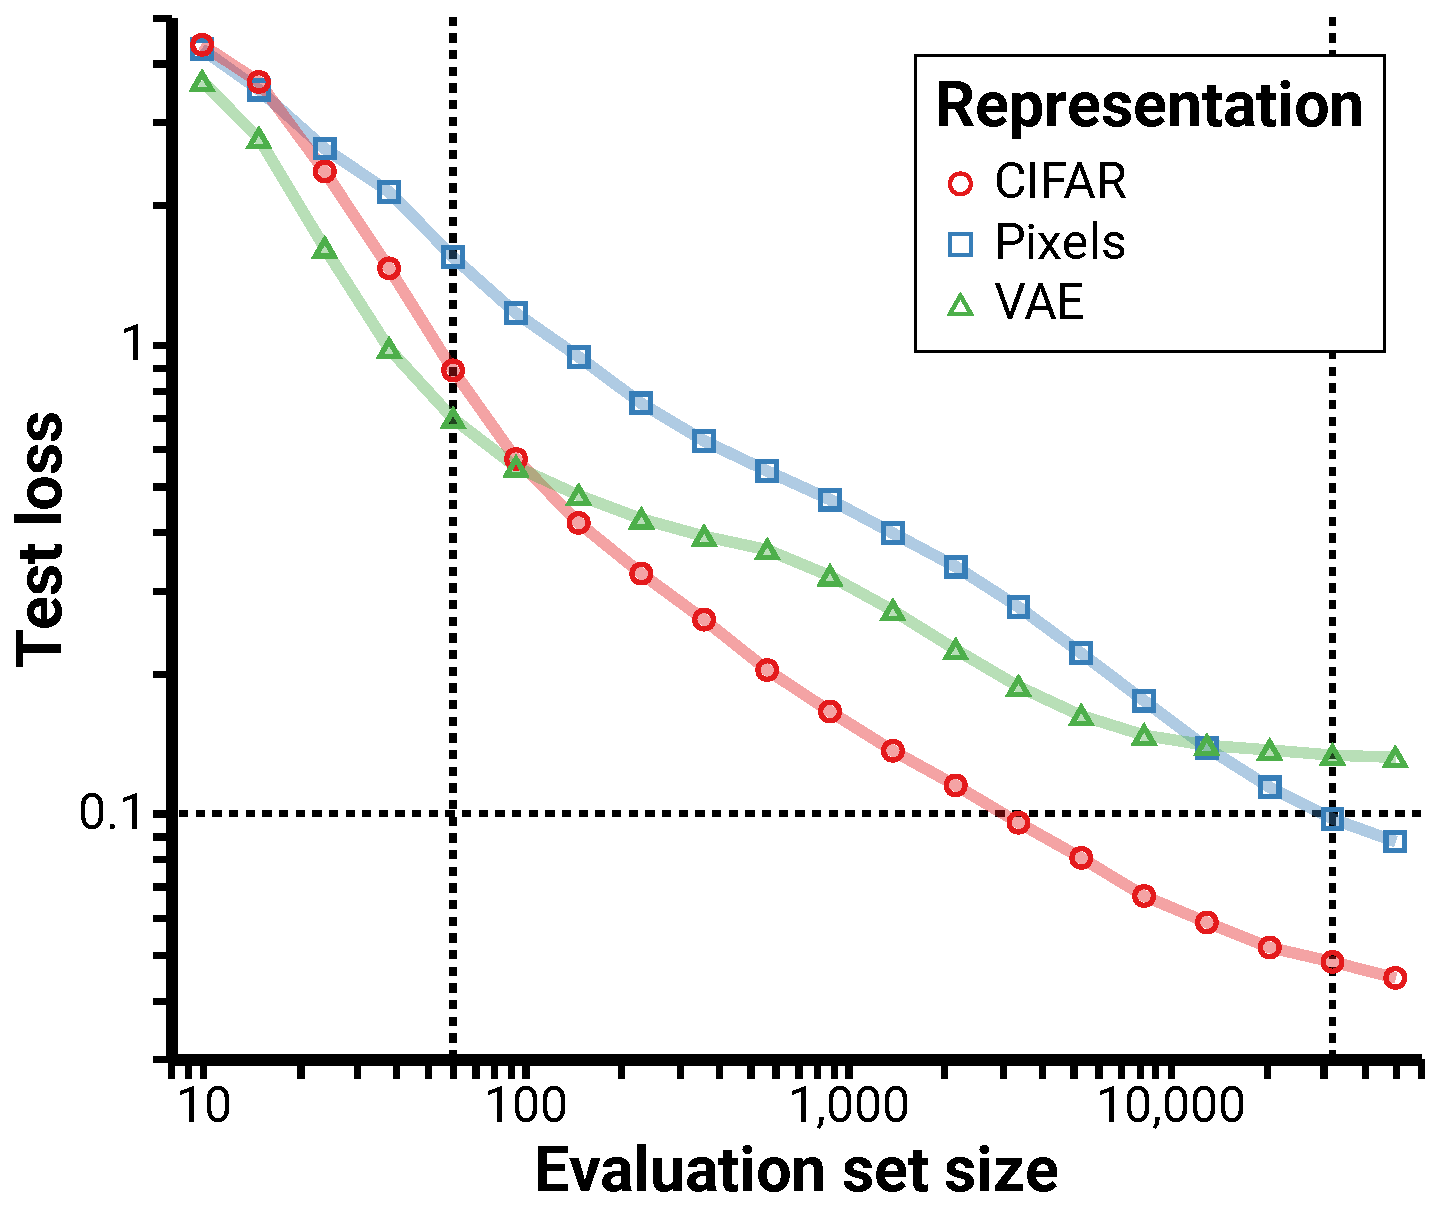
\includegraphics[width=0.45\textwidth]{figures/repr-eval/mnist_reprs_fixedloss_oneeps.pdf}
  \caption{Results using three representations on MNIST.
  The intersections between curves indicate evaluation dataset sizes where VA would change its ranking of these representations. Curves are estimated using eight bootstrap-sampled evaluation datasets and initializations at each point to ensure the measured quantities are close to the expectation.}
  \label{fig:multi_mnist}
\end{figure}

\begin{table}[th]
    \centering
    {\small
\begin{tabular}{llabc}
\toprule
      & Representation &     CIFAR &    Pixels &      VAE \\
n & {} &           &           &          \\
\midrule
60    & VA &      0.88 &      1.54 &       \textbf{0.70} \\
      & MDL &    122.75 &    147.34 &       \textbf{93.8} \\
      & SDL, $\varepsilon$=0.1 &  > 116.75 &  > 141.34 &     > 87.8 \\
      & $\varepsilon$SC, $\varepsilon$=0.1 &    > 60.0 &    > 60.0 &     > 60.0 \\
31936 & VA &      \textbf{0.05} &      0.10 &       0.13 \\
      & MDL &    \textbf{2165.1} &   5001.57 &    4898.37 \\
      & SDL, $\varepsilon$=0.1 &     \textbf{260.6} &   1837.08 &  > 1704.77 \\
      & $\varepsilon$SC, $\varepsilon$=0.1 &      \textbf{3395} &     31936 &  > 31936.0 \\
\bottomrule
\end{tabular}
}
    \caption{Estimated measures of representation quality on MNIST. At small evaluation dataset sizes, VA and MDL state that the VAE representation is the best, even though every representation yields poor prediction quality with that amount of data. Since SDL and $\eps$SC have a target for prediction quality, they are able to report when the evaluation dataset is insufficient to achieve the desired performance.}
    \label{tab:multi_mnist}
\end{table}

\subsection{Tasks and representations}
For the first experiment, shown in \Cref{fig:multi_mnist} and \Cref{tab:multi_mnist}, we use the small-scale task of MNIST classification.
We evaluate three representations: (1) the last hidden layer of a small convolutional network pretrained on CIFAR-10; (2) the raw pixels; and (3) the bottleneck of a variational autoencoder (VAE) \citep{Kingma2014AutoEncodingVB,Rezende2014StochasticBA} trained on MNIST.


For the second experiment, shown in \Cref{fig:elmo_layers} and \Cref{tab:elmo_layers}, we compare the representations given by different layers of a pretrained ELMo model \citep{Peters2018DeepCW}.
We use the part-of-speech task introduced by \citet{Hewitt2019DesigningProbes} and implemented by \citet{Voita2020InformationTheoreticPW} with the same probe architecture and other hyperparameters as those works.
This leads to a large-scale representation evaluation task, with 4096-dimensional representation vectors and an output space of size $48^k$ for a sentence of $k$ words.

In each set of experiments we compute loss-data curves by estimating the expected population loss at each evaluation dataset size using a bootstrapped sample from the full evaluation dataset, reducing the variance of the results.
Note that in each experiment we omit MI as for a finite evaluation dataset, the MI measure is the same as validation loss.
Details of the experiments, including representation training, probe architectures, and hyperparameters, are available in Appendix \ref{sec:experiment_details}.

\subsection{Results}
These experiments demonstrate that the issue of sensitivity to evaluation dataset size in fact occurs in practice, both on small problems (\Cref{tab:multi_mnist}) and at scale (\Cref{tab:elmo_layers}): VA and MDL choose different representations when given evaluation sets of different sizes.
Because these measures are a function of the evaluation dataset size, making a decision about which representation to use with a small evaluation dataset would be premature.

By contrast, SDL and $\eps$SC are functions only of the data \emph{distribution}, not a finite sample.
Once they measure the complexity of learning an $\eps$-loss function, that measure is invariant to the size of the evaluation dataset.
Crucially, since these measures contain a notion of success in  solving a task, they are able to avoid the issue of premature evaluation and notify the user if there is insufficient data to evaluate and return a lower bound instead.

The part of speech experiment in \Cref{fig:elmo_layers} and \Cref{tab:elmo_layers} demonstrates that SDL and $\eps$SC can scale to tasks of a practically relevant size.
This experiment is of a similar size to the widespread use of BERT \citep{devlin2018bert} or SimCLR \citep{Chen2020ASF}, and evaluating our measures to high precision took about an hour on one GPU.

\begin{figure}[tb]
\centering
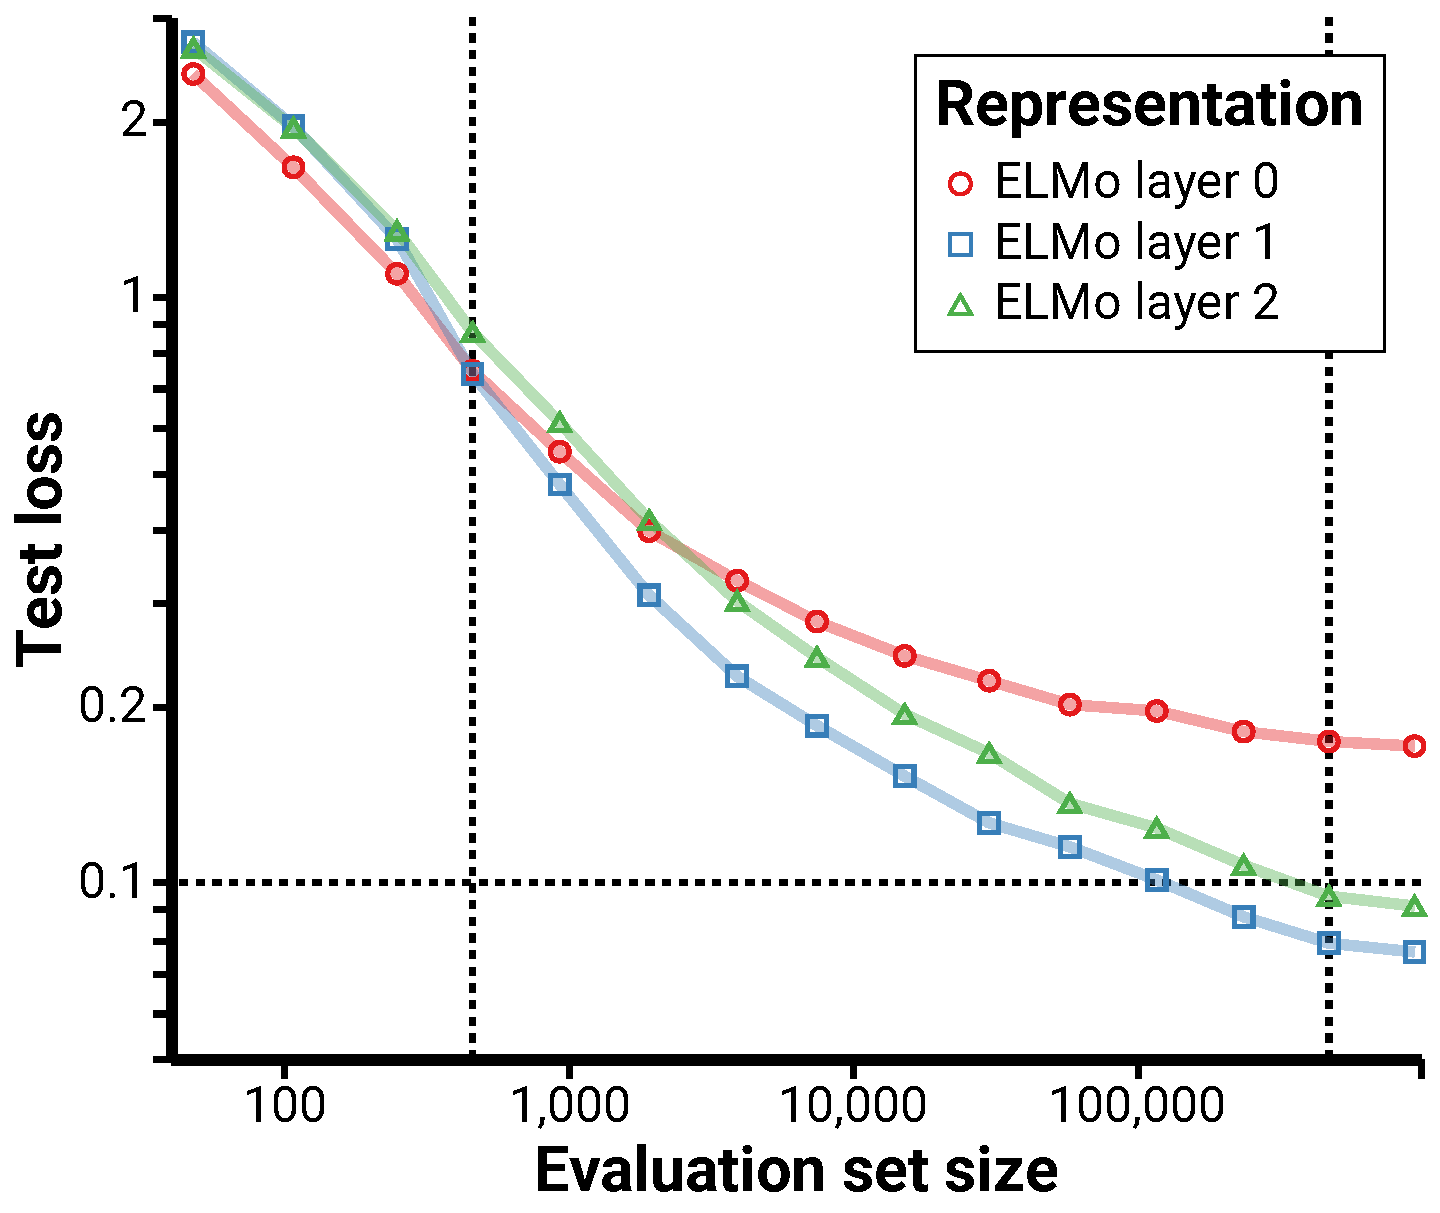
\includegraphics[width=0.45\textwidth]{figures/repr-eval/elmo_layers_oneeps.pdf}
\caption{Results using three representations on the part of speech classification task. Loss-data curves are estimated using four bootstrap-sampled evaluation datasets and network initializations at each point.}
\label{fig:elmo_layers}
\end{figure}

\begin{table}[tb]
    \centering
    {\small
\begin{tabular}{llabc}
\toprule
       & ELMo layer &           0 &         1 &         2 \\
n & {} &             &           &           \\
\midrule
461    & VA &        0.75 &      \textbf{0.74} &     0.87 \\
       & MDL &      \textbf{884.54} &   1009.26 &  1017.72 \\
       & SDL, $\varepsilon$=0.1 &    > 478.67 &  > 528.51 &  > 561.7 \\
       & $\varepsilon$SC, $\varepsilon$=0.1 &       > 461 &     > 461 &    > 461 \\
474838 & VA &        0.17 &      \textbf{0.08} &     0.09 \\
       & MDL &    92403.41 &  \textbf{52648.50} & 65468.54 \\
       & SDL, $\varepsilon$=0.1 &  > 40882.72 &   \textbf{2765.11} &  7069.56 \\
       & $\varepsilon$SC, $\varepsilon$=0.1 &    > 474838 &    \textbf{237967} &   474838 \\
\bottomrule
\end{tabular}
}
    \caption{Estimated measures of representation quality on the part of speech classification task. With small evaluation datasets, MDL finds that the lowest ELMo layer gives the best results, but when the evaluation dataset grows the outcome changes.}
    \label{tab:elmo_layers}
\end{table}



\section{Related work}

\paragraph{Representation evaluation methods.}
Until recently, the standard technique for evaluating representation quality was the use of linear probes \citep{Kiros2015SkipThoughtV,Hill2016LearningDR,Oord2018RepresentationLW,Chen2020ASF}.
However, \citet{Hnaff2020DataEfficientIR} find that evaluation with linear probes is largely uncorrelated with the more practically relevant objective of low-data accuracy, and \citet{resnick2019probing} show that linear probe performance does not predict performance for transfer across tasks.
Beyond linear probes, \citet{Zhang2018LanguageMT} and \citet{Hewitt2019DesigningProbes} show that restrictions on model capacity or evaluation dataset size are necessary to separate the performance of randomly- and linguistically-pretrained representations.
\citet{Voita2020InformationTheoreticPW} propose using the MDL framework, which
measures the description length of the labels given the observations.
An earlier work by~\citet{Yogatama2019LinguisticIntel} also uses prequential codes to evaluate representations for linguistic tasks.
\citet{Talmor2019oLMpics} look at the loss-data curve (called ``learning curve'' in their work) and use a weighted average of the validation loss at various training set sizes to evaluate representations.

\paragraph{Foundational work.}
A fundamental paper by \citet{Blier2018TheDL} introduces prequential codes as a measure of the complexity of a deep learning model.
\citet{Xu2020ATheory} introduce predictive $\mathcal{V}$-information, a theoretical generalization of mutual information which takes into account computational constraints,
and is essentially the mutual information lower bound often reported in practice.
Work by \citet{Dubois2020LearningOR} describe representations which, in combination with a specified family of predictive functions, have guarantees on their generalization performance.


\section{Discussion}

In this work, we have introduced the loss-data framework for comparing representation evaluation measures and used it to diagnose the issue of sensitivity to evaluation dataset size in the validation accuracy and minimum description length measures.
We proposed two measures, surplus description length and $\eps$ sample complexity, which eliminate this issue by measuring the complexity of learning a predictor which solves the task of interest to $\eps$ tolerance.
Empirically, we showed that sensitivity to evaluation dataset size occurs in practice for VA and MDL, while SDL and $\eps$SC are robust to the amount of available data and are able to report when it is insufficient to make a judgment.

Each of these measures depends on a choice of algorithm $\mathcal{A}$, including hyperparameters such as probe architecture, which could make the evaluation procedure less robust.
To alleviate this, future work might consider a set of algorithms $A = \{\mathcal{A}_i\}_{i=1}^K$ and a method of combining them, such as the model switching technique of \citet{Blier2018TheDL,Erven2012CatchingUF} or a Bayesian prior.

Finally, while existing measures such as VA, MI, and MDL do not measure our notion of the best representation for a task, under other settings they may be the correct choice.
For example, if only a fixed set of data will ever be available, selecting representations using VA might be a reasonable choice; and if unbounded data is available for free, perhaps MI is the most appropriate measure.
However, in many cases the robustness and interpretability offered by SDL and $\eps$SC make them a practical choice for practitioners and representation researchers alike.


\clearpage
\begin{subappendices}
% \newappendix{Algorithmic details for estimating surplus description length} \label{sec:sdl_details}

% Recall that the SDL is defined as
% \begin{align}
%         m_{\mathrm{SDL}}(\phi, \mathcal{D}, \mathcal{A},\eps) &= \sum_{n=1}^\infty \Big[ L(\mathcal{A}_\phi, n) - \eps \Big]_+
% \end{align}
% For simplicity, we assume that $L$ is bounded in $[0,1]$. Note that this can be achieved by truncating the cross-entropy loss.

% \begin{algorithm}
% \caption{Estimate surplus error}
% \label{alg:sdl}
% \KwIn{tolerance $\eps $, max iterations $M$, number of datasets $K$, representation $ \phi$, data distribution $\mathcal{D}$, algorithm $\mathcal{A}$ }
% \KwOut{Estimate $\hat m $ of  $m(\phi, \mathcal{D}, \eps, \mathcal{A})$ and indicator $ I$ of whether this estimate is tight or lower bound}
% \vspace{1mm} \hrule \vspace{1mm}
% Sample $ K$ datasets $ D_M^{k}\sim \mathcal{D}$ of size $ M+1$\\
% \For{$n = 1$ \KwTo $M$}{
%     For each $ k \in [K]$, run $ \mathcal{A}$ on $ D_M^{k}[1:n]$ to produce a predictor $ \hat p_n^k$\\
%     Take $ K $ test samples $ (x_k, y_k) = D_M^k[M+1]$\\
%     Evaluate $ \hat L_n = \frac{1}{K}\sum_{k=1}^K \ell(\hat p_n^k, x_k , y_k) $
%     }
% Set $ \hat m = \sum_{n=1}^M [\hat L_n - \eps]_+$ \vspace{1mm}\\
% \lIf {$ \hat L_M \leq \eps/2$} {Set $I = $ \texttt{tight} \textbf{else} {Set $ I = $ \texttt{lower bound}}}
% \Return $\hat m, I$
% \end{algorithm}

% In our experiments we replace $D^k_M[1:n]$ of Algorithm \ref{alg:sdl} with sampled subsets of size $n$ from a single evaluation dataset.
% Additionally, we use between 10 and 20 values of $n$ instead of evaluating $L(\mathcal{A}_\phi, n)$ at every integer between $1$ and $M$.
% This strategy, also used by \citet{Blier2018TheDL} and \citet{Voita2020InformationTheoreticPW}, corresponds to the description length under a code which updates only periodically during transmission of the data instead of after every single point.

% \begin{theorem}
% Let the loss function $L$ be bounded in $[0,1]$ and assume that it is decreasing in $ n$. With $ (M+1)K $ datapoints, if the sample complexity is less than $ M$, the above algorithm returns an estimate $ \hat m$ such that with probability at least $ 1- \delta$
% \begin{align}
%     |\hat m - m(\phi, \mathcal{D}, \eps, \mathcal{A})| \leq  M\sqrt{ \frac{\log (2M/\delta)}{2K}}.
% \end{align}
% If $ K \geq \frac{\log(1/\delta)}{2\eps^2}$ and the algorithm returns \texttt{tight} then with probability at least $ 1-\delta$ the sample complexity is less than $ M $ and the above bound holds.
% \end{theorem}
% \begin{proof}
% First we apply a Hoeffding bound to show that each $ \hat L_n$ is estimated well. For any $ n$, we have
% \begin{align}
%     P \bigg( \big|\hat L_n   - L(\mathcal{A}_\phi,n)  \big| > \sqrt{\frac{\log(2M/\delta)}{2K}} \bigg) \leq 2 \exp\bigg(-2K  \frac{\log(2M/\delta)}{2K}\bigg) = 2 \frac{\delta}{2M} = \frac{\delta}{M}
% \end{align}
% since each $ \ell(\hat p_n^k, x_k , y_k)$ is an independent variable, bounded in [0,1] with expectation $ L(\mathcal{A}_\phi, n)$.

% Now when sample complexity is less than $ M$, we use a union bound to translate this to a high probability bound on error of $ \hat m$, so that with probability at least $ 1- \delta$:
% \begin{align}
%     |\hat m - m(\phi, \mathcal{D}, \eps, \mathcal{A})| &= \bigg|\sum_{n=1}^M [\hat L_n - \eps]_+  - [L(\mathcal{A}_\phi,n) - \eps]_+  \bigg|\\
%     &\leq \sum_{n=1}^M\bigg| [\hat L_n - \eps]_+  - [L(\mathcal{A}_\phi,n) - \eps]_+ \bigg|\\
%     &\leq \sum_{n=1}^M \bigg|\hat L_n - L(\mathcal{A}_\phi,n) \bigg|\\
%     &\leq M \sqrt{ \frac{\log (2M/\delta)}{2K}}
% \end{align}
% This gives us the first part of the claim.

% We want to know that when the algorithm returns \texttt{tight}, the estimate can be trusted (i.e. that we set $ M $ large enough). Under the assumption of large enough $K$, and by an application of Hoeffding, we have that
% \begin{align}
%     P \bigg(  L(\mathcal{A}_\phi,M) - \hat L_M  > \eps/2 \bigg) \leq  \exp\bigg(-2K \eps^2 \bigg) \leq  \exp\bigg(-2 \frac{\log(1/\delta)}{2\eps^2} \eps^2 \bigg) = \delta
% \end{align}
% If $ \hat L_M \leq \eps/2$, this means that $ L(\mathcal{A}_\phi,M) \leq \eps$ with probability at least $ 1-\delta$. By the assumption of decreasing loss, this means the sample complexity is less than $ M$, so the bound on the error of $ \hat m$ holds.
% \end{proof}



% \newappendix{Algorithmic details for estimating sample complexity} \label{sec:sc_details}
% Recall that $\eps$ sample complexity ($\eps$SC) is defined as
% \begin{align}
%      m_{\eps\mathrm{SC}}(\phi, \mathcal{D}, \mathcal{A},\eps) &= \min \Big\{ n \in \mathbb{N} : L(\mathcal{A}_\phi, n) \leq \eps \Big\}.
% \end{align}

% We estimate $m_{\eps\mathrm{SC}}$ via recursive grid search. To be more precise, we first define a search interval $[1,N]$, where $N$ is a large enough number such that $L(\mathcal{A}_\phi,N) \ll \eps$. Then, we partition the search interval in to 10 sub-intervals and estimate risk of hypothesis learned from $D^n \sim \mathcal{D}^n$ with high confidence for each sub-interval. We then find the leftmost sub-interval that potentially contains $m_{\eps\mathrm{SC}}$ and proceed recursively. This procedure is formalized in Algorithm~\ref{alg:esc} and its guarantee is given by Theorem~\ref{thm:esc}.
% \begin{algorithm}[h!]
% \caption{Estimate sample complexity via recursive grid search}
% \label{alg:esc}
% \KwIn{Search upper limit $N$, parameters $\eps$, confidence parameter $\delta$, data distribution $\mathcal{D}$, and learning algorithm $\mathcal{A}$.}
% \KwOut{Estimate $\hat{m}$ such that $m_{\eps\mathrm{SC}}(\phi,\mathcal{D},\mathcal{A},\eps) \le \hat m$ with probability $1-\delta$.}
% \vspace{1mm} \hrule \vspace{1mm}
% let $S = 2\log (20k/\delta)/\eps^2$, and let $[\ell,u]$ be the search interval initialized at $\ell = 1, u = N$.\\
% \For{$r=1$ \KwTo $k$}{
%     Partition $[\ell,u]$ into 10 equispaced bins and let $\Delta$ be the length of each bin. \\
%     \For{$j = 1$ \KwTo $10$}{
%         Set $n = \ell + j \Delta$. \\
%         Compute $\hat L_n = \frac{1}{S}\sum_{i=1}^S \ell(\mathcal{A}(D^n_i),x_i,y_i)$ for $S$ independent draws of $D^n$ and test sample $(x,y)$. \\
%         \If{$\hat L_n \le \eps/2$}{
%         Set $u = n$ and $\ell = n - \Delta$. \\
%         \textbf{break}
%         }
%         }
% }
% \Return $\hat m = u$, which satisfies $m_{\eps\mathrm{SC}}(\phi,\mathcal{D},\mathcal{A},\eps) \le \hat m$ with probability $1-\delta$, where the randomness is over independent draws of $D^n$ and test samples $(x,y)$.
% \end{algorithm}

% \begin{theorem}
% \label{thm:esc}
% Let the loss function $L$ be bounded in $[0,1]$ and assume that it is decreasing in $ n$. Then, Algorithm~\ref{alg:esc} returns an estimate $ \hat m$ that satisfies $m_{\eps\mathrm{SC}}(\phi,\mathcal{D},\mathcal{A},\eps) \le \hat m$ with probability at least $ 1- \delta$.
% \end{theorem}

% \begin{proof}
% By Hoeffding, the probability that $|\hat L_n-L(\mathcal{A}_{\phi},n)| \ge \eps/2$, where $\hat L$ is computed with $S = 2\log(20k/\delta)/\eps^2$ independent draws of $D^n \sim \mathcal{D}^n$ and $(x,y) \sim \mathcal{D}$, is less than $\delta/(10k)$. The algorithm terminates after evaluating $\hat L$ on at most $10k$ different $n$'s. By a union bound, the probability that $|\hat L_n - L(\mathcal{A}_{\phi},n)| \le \eps/2$ for all $n$ used by the algorithm is at least $1-\delta$. Hence, $\hat L_n \le \eps/2$ implies $L(\mathcal{A}_\phi,n) \le \eps$ with probability at least $1-\delta$.
% \end{proof}

\newappendix{Experimental details} \label{sec:experiment_details}

In each experiment we first estimate the loss-data curve using a fixed number of dataset sizes $n$ and multiple random seeds, then compute each measure from that curve.
Reported values of SDL correspond to the estimated area between the loss-data curve and the line $y=\eps$ using Riemann sums with the values taken from the left edge of the interval.
This is the same as the chunking procedure of \citet{Voita2020InformationTheoreticPW} and is equivalent to the code length of transmitting each chunk of data using a fixed model and switching models between intervals.
Reported values of $\eps$SC correspond to the first measured $n$ at which the loss is less than $\eps$.

All of the experiments were performed on a single server with 4 NVidia Titan X GPUs, and on this hardware no experiment took longer than an hour.
All of the code for our experiments, as well as that used to generate our plots and tables, is included in the supplement.


\subsection{MNIST experiments}

For our experiments on MNIST, we implement a highly-performant vectorized library in \hyperlink{https://jax.readthedocs.io/en/latest/}{JAX} to construct loss-data curves.
With this implementation it takes about one minute to estimate the loss-data curve with one sample at each of 20 settings of $n$.
We approximate the loss-data curves at 20 settings of $n$ log-uniformly spaced on the interval $[10, 50000]$ and evaluate loss on the test set to approximate the population loss.
At each dataset size $n$ we perform the same number of updates to the model; we experimented with early stopping for smaller $n$ but found that it made no difference on this dataset.
In order to obtain lower-variance estimates of the expected risk at each $n$, we run 8 random seeds for each representation at each dataset size, where each random seed corresponds to a random initialization of the probe network and a random subsample of the evaluation dataset.

Probes consist of two-hidden-layer MLPs with hidden dimension 512 and ReLU activations.
All probes and representations are trained with the Adam optimizer \citep{Kingma2015AdamAM} with learning rate $10^{-4}$.

Each representation is normalized to have zero mean and unit variance before probing to ensure that differences in scaling and centering do not disrupt learning.
The representations of the data we evaluate are implemented as follows.

\paragraph{Raw pixels.}
The raw MNIST pixels are provided by the Pytorch \texttt{datasets} library \citep{Paszke2019PyTorchAI}.
It has dimension $28 \times 28 = 784$.

\paragraph{CIFAR.}
The CIFAR representation is given by the last hidden layer of a convolutional neural network trained on the CIFAR-10 dataset.
This representation has dimension 784 to match the size of the raw pixels.
The network architecture is as follows:

\begin{verbatim}
    nn.Conv2d(1, 32, 3, 1),
    nn.ReLU(),
    nn.MaxPool2d(2),
    nn.Conv2d(32, 64, 3, 1),
    nn.ReLU(),
    nn.MaxPool2d(2),
    nn.Flatten(),
    nn.Linear(1600, 784)
    nn.ReLU()
    nn.Linear(784, 10)
    nn.LogSoftmax()
\end{verbatim}

\paragraph{VAE.}
The VAE (variational autoencoder; \citet{Kingma2014AutoEncodingVB,Rezende2014StochasticBA}) representation is given by a variational autoencoder trained to generate the MNIST digits.
This VAE's latent variable has dimension 8.
We use the mean output of the encoder as the representation of the data.
The network architecture is as follows:
\begin{verbatim}
self.encoder_layers = nn.Sequential(
    nn.Linear(784, 400),
    nn.ReLU(),
    nn.Linear(400, 400),
    nn.ReLU(),
    nn.Linear(400, 400),
    nn.ReLU(),
)
self.mean = nn.Linear(400, 8)
self.variance = nn.Linear(400, 8)

self.decoder_layers = nn.Sequential(
    nn.Linear(8, 400),
    nn.ReLU(),
    nn.Linear(400, 400),
    nn.ReLU(),
    nn.Linear(400, 784),
)
\end{verbatim}

\subsection{Part of speech experiments}

We follow the methodology and use the official code\endnote{Code available at \url{https://github.com/lena-voita/description-length-probing}.} of \citet{Voita2020InformationTheoreticPW} for our part of speech experiments using ELMo \citep{Peters2018DeepCW} pretrained representations.
In order to obtain lower-variance estimates of the expected risk at each $n$, we run 4 random seeds for each representation at each dataset size, where each random seed corresponds to a random initialization of the probe network and a random subsample of the evaluation dataset.
We approximate the loss-data curves at 10 settings of $n$ log-uniformly spaced on the range of the available data $n \in [10, 10^6]$.
To more precisely estimate $\eps$SC, we perform one recursive grid search step: we space 10 settings over the range which in the first round saw $L(\mathcal{A}_\phi, n)$ transition from above to below $\eps$.

Probes consist of the MLP-2 model of \citet{Hewitt2019DesigningProbes,Voita2020InformationTheoreticPW} and all training parameters are the same as in those works.
\end{subappendices}
\printendnotes

\chapter{Dynamics-Aware Embeddings} \label{sec:dyne}
\section{Introduction}

In recent years, there has been a lot of excitement around end-to-end model-free reinforcement learning for control, both in simulation \citep{lillicrap2015continuous, andrychowicz2018learning, haarnoja2018soft, fujimoto2018addressing} and on real hardware \citep{kalashnikov2018qt, haarnoja2018softapp}.
In this paradigm, we simultaneously learn intermediate representations and policies by maximizing rewards provided by environment.
End-to-end learning has one indisputable advantage: since every component of the system is optimized for the end objective, there are no sub-optimal modules that limit best-case performance by losing task-relevant information.

Learning only from the target task is however a double-edged sword.
When the end objective provides only weak signal for learning, a policy with a poor representation may require many samples to learn a better one.
By contrast, a policy with a good representation may be able to rapidly fit a simple function of that representation even with weak signal.



\begin{figure}[h]
    \centering
    % \vspace{-10pt}
    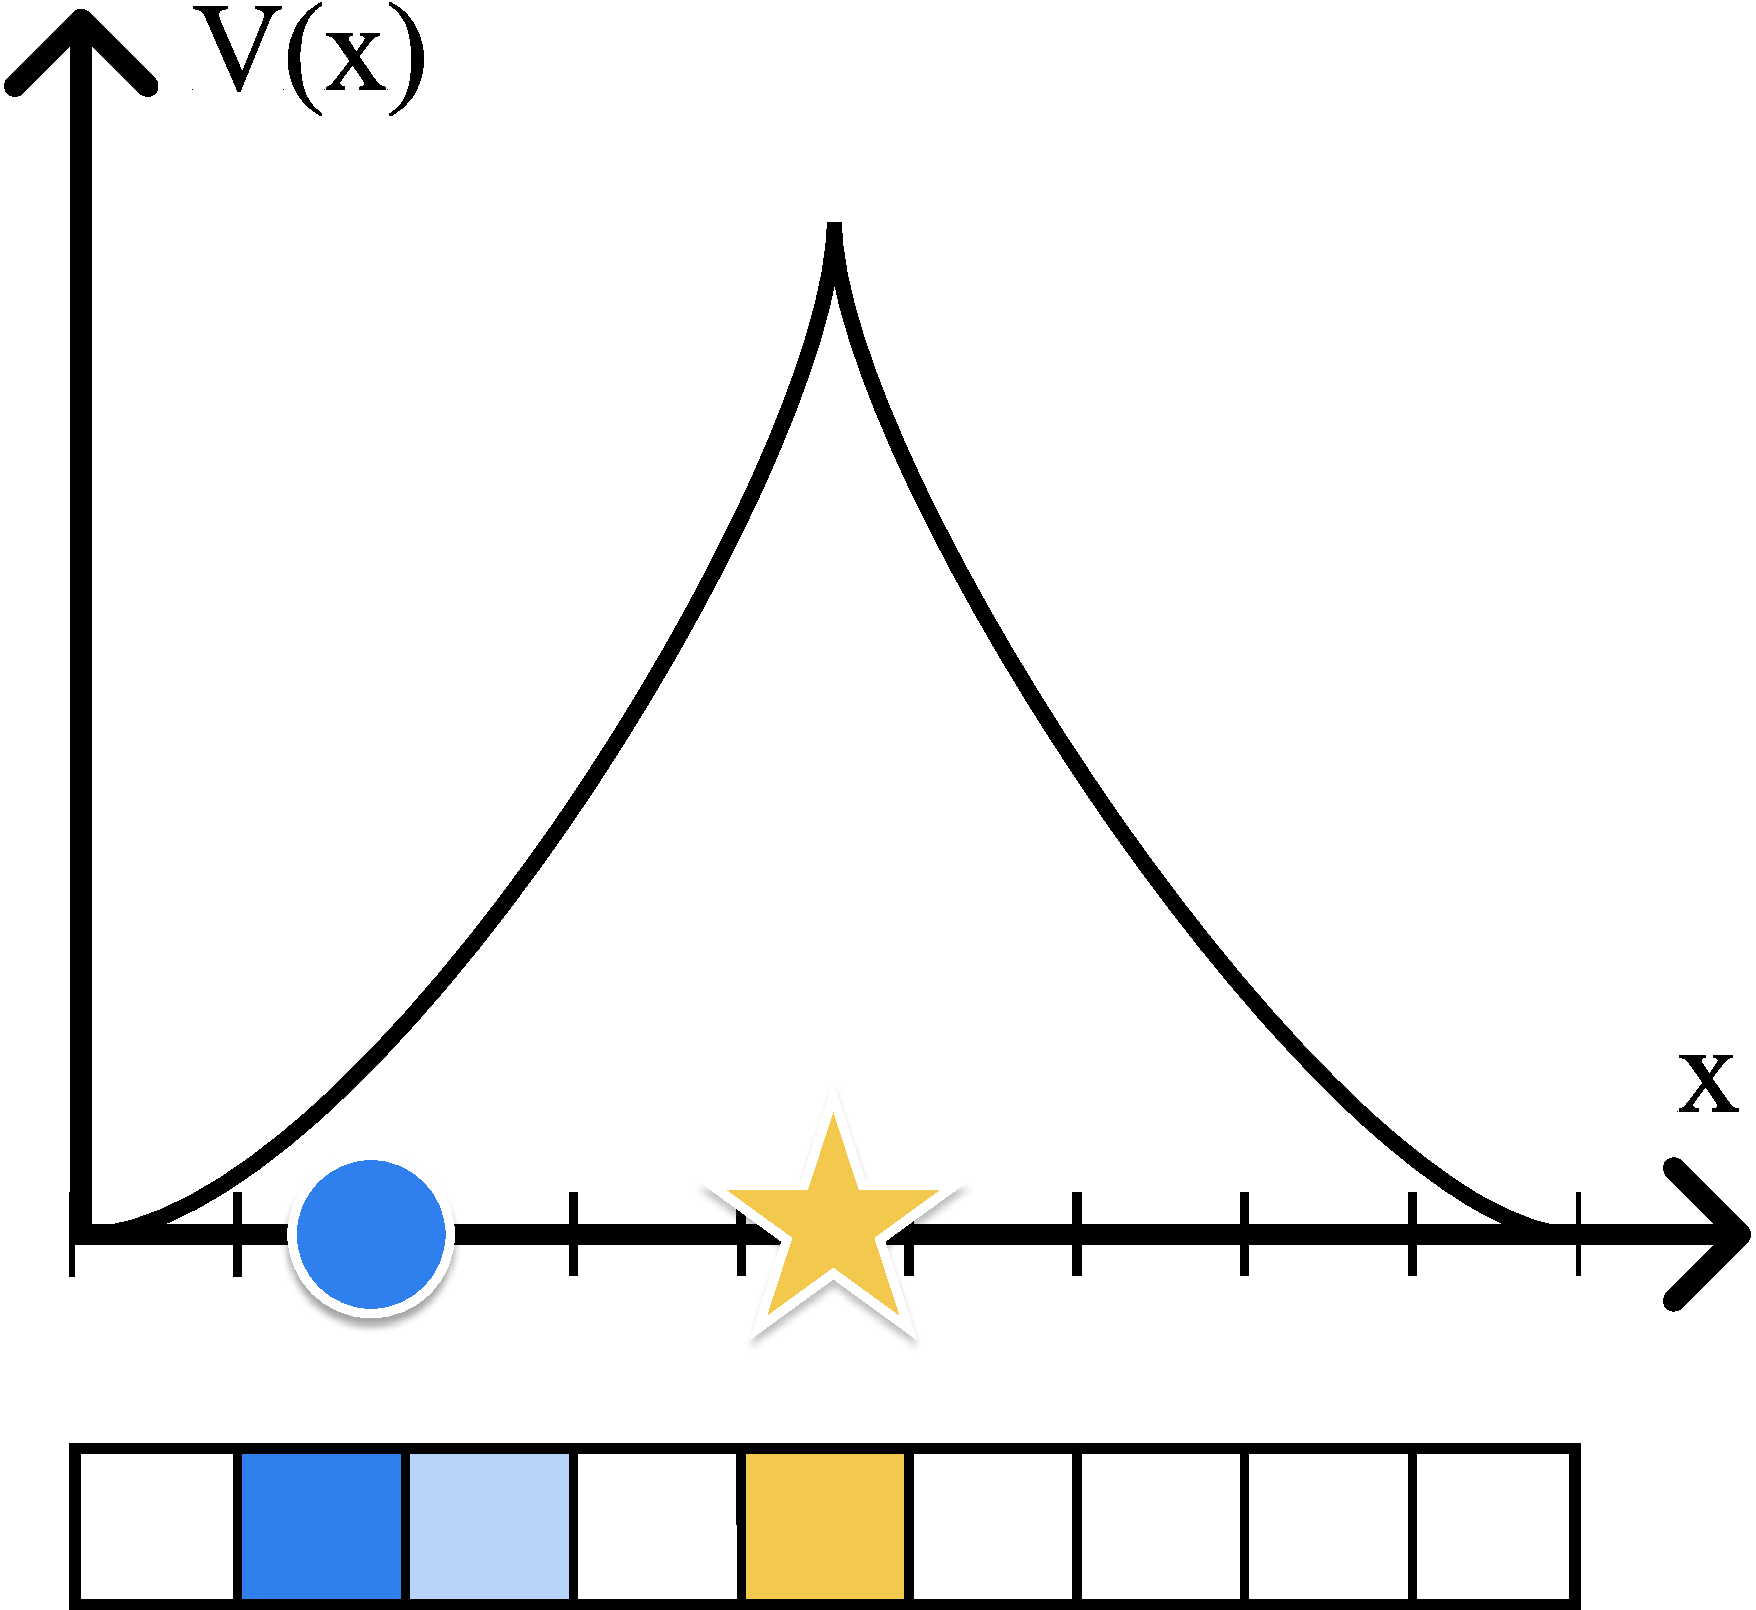
\includegraphics[width=0.4\textwidth]{figures/dyne/env_illustration_1d.pdf}
    \caption{A 1D environment. The agent (blue dot) can move continuously left and right to reach the goal (gold star).}
    \label{fig:pixel_illustration}
    % \vspace{-10pt}
\end{figure}

Consider the environment shown in \Cref{fig:pixel_illustration}, and two representations of its state: coordinates and pixels.
As a function of the agent's $x$ coordinate, the value function is simple and smooth.
The coordinate representation has structure which is useful for learning about the task; namely, points which are close in $L^2$ distance have similar values.
By contrast, a pixel representation of the agent's state (below, blue) is practically a one-hot vector.
Two states whose $x$ coordinates differ by one unit have pixels exactly as different as states which differ by 100 units.
This illustrates the importance of good representations and the potential of representation learning to aid RL.

% In this work, we consider the problem of self-supervised representation learning for reinforcement learning.
% % Our key insight is that the difference between two states or two actions should be measured by the difference in their effects on the environment.
% Our contributions are as follows:
%
% \begin{enumerate}
%     % \item We describe a set of goals that representations in RL should aim to achieve, providing a framework for analyzing a representation's strengths and weaknesses.
%     \item We construct a representation learning objective that captures the structure of the dynamics. This objective, called Dynamics-aware Embedding or DynE, yields embeddings where nearby states and actions have similar outcomes.
%     \item We show that this single objective greatly simplifies learning from pixels and enables faster exploration through temporally abstract actions.
% \end{enumerate}

% In this work, we turn this intuition into an objective
 % consider the problem of self-supervised representation learning for reinforcement learning.
% We propose to learn embeddings of states and actions such that a pair of states or actions will only be close together if they have similar
We propose a self-supervised objective for learning embeddings of states and action sequences such that a pair of states or action sequences will be close together if they have similar outcomes.
% This addresses the difficulty depicted in \Cref{fig:pixel_illustration} by constructing a smooth representation from a difficult one (e.g. pixels).
% Simultaneously our objective provides a principle for learning a temporally abstract action space for control which is task-independent and generalizes across goals and objects to interact with.
This objective simultaneously trains a smooth embedding space for states and a temporally abstract action space for control which is task-independent and generalizes across goals and objects.

% which is task-independent and remains valid
% which we show leads to faster policy learning in environments which require exploration.
% This abstract action space

We demonstrate the effectiveness of our representation learning objective by training the twin delayed deep deterministic policy gradient algorithm (TD3) \citep{fujimoto2018addressing} with learned action and state spaces.
With a learned representation of temporally abstract actions, our method exhibits improved sample efficiency compared to state-of-the-art RL methods on control tasks, with larger gains on more complex environments.
When additionally combined with our learned state representation, our method allows TD3 to scale to pixel observations.
We demonstrate good performance on a simple family of goal-conditioned 2D control tasks within a few million environment steps without adjusting any TD3 hyperparameters.
This stands in contrast to end-to-end model-free RL from pixels, which requires extensive tuning \citep{lillicrap2015continuous} and on the order of 100 million environment steps\endnote{Number of steps required to train D4PG taken from \citet{hafner2018learning}, as \citet{barth2018distributed} does not include this information.} \citep{barth2018distributed}.





\section{Dynamics-aware embeddings}

\subsection{Notation}

We consider the framework of reinforcement learning in Markov decision processes (MDPs).\endnote{In the interest of space we omit the usual recap of Markov decision processes and reinforcement learning.
We refer the reader to Section 2 of \citet{silver2014deterministic} for notation and background on MDPs.}
We denote the state of an environment (e.g.\ joint angles of a robot or pixels) by $s \in \mathcal{S}$, and we assume that the states given by the environment satisfy the Markov property.
We refer to a sequence of actions $\{ a_1, \ldots, a_k \} \in \mathcal{A}^k$ using the shorthand $\va^k$.
We use $s' \sim \trans(s, a)$ to refer to the environment's (stochastic) transition function, and overload it to accept sequences of actions: $s_{t+k} \sim \trans(s_t, \va^k_t)$.


\subsection{Model and learning objective}

\begin{figure}[t]
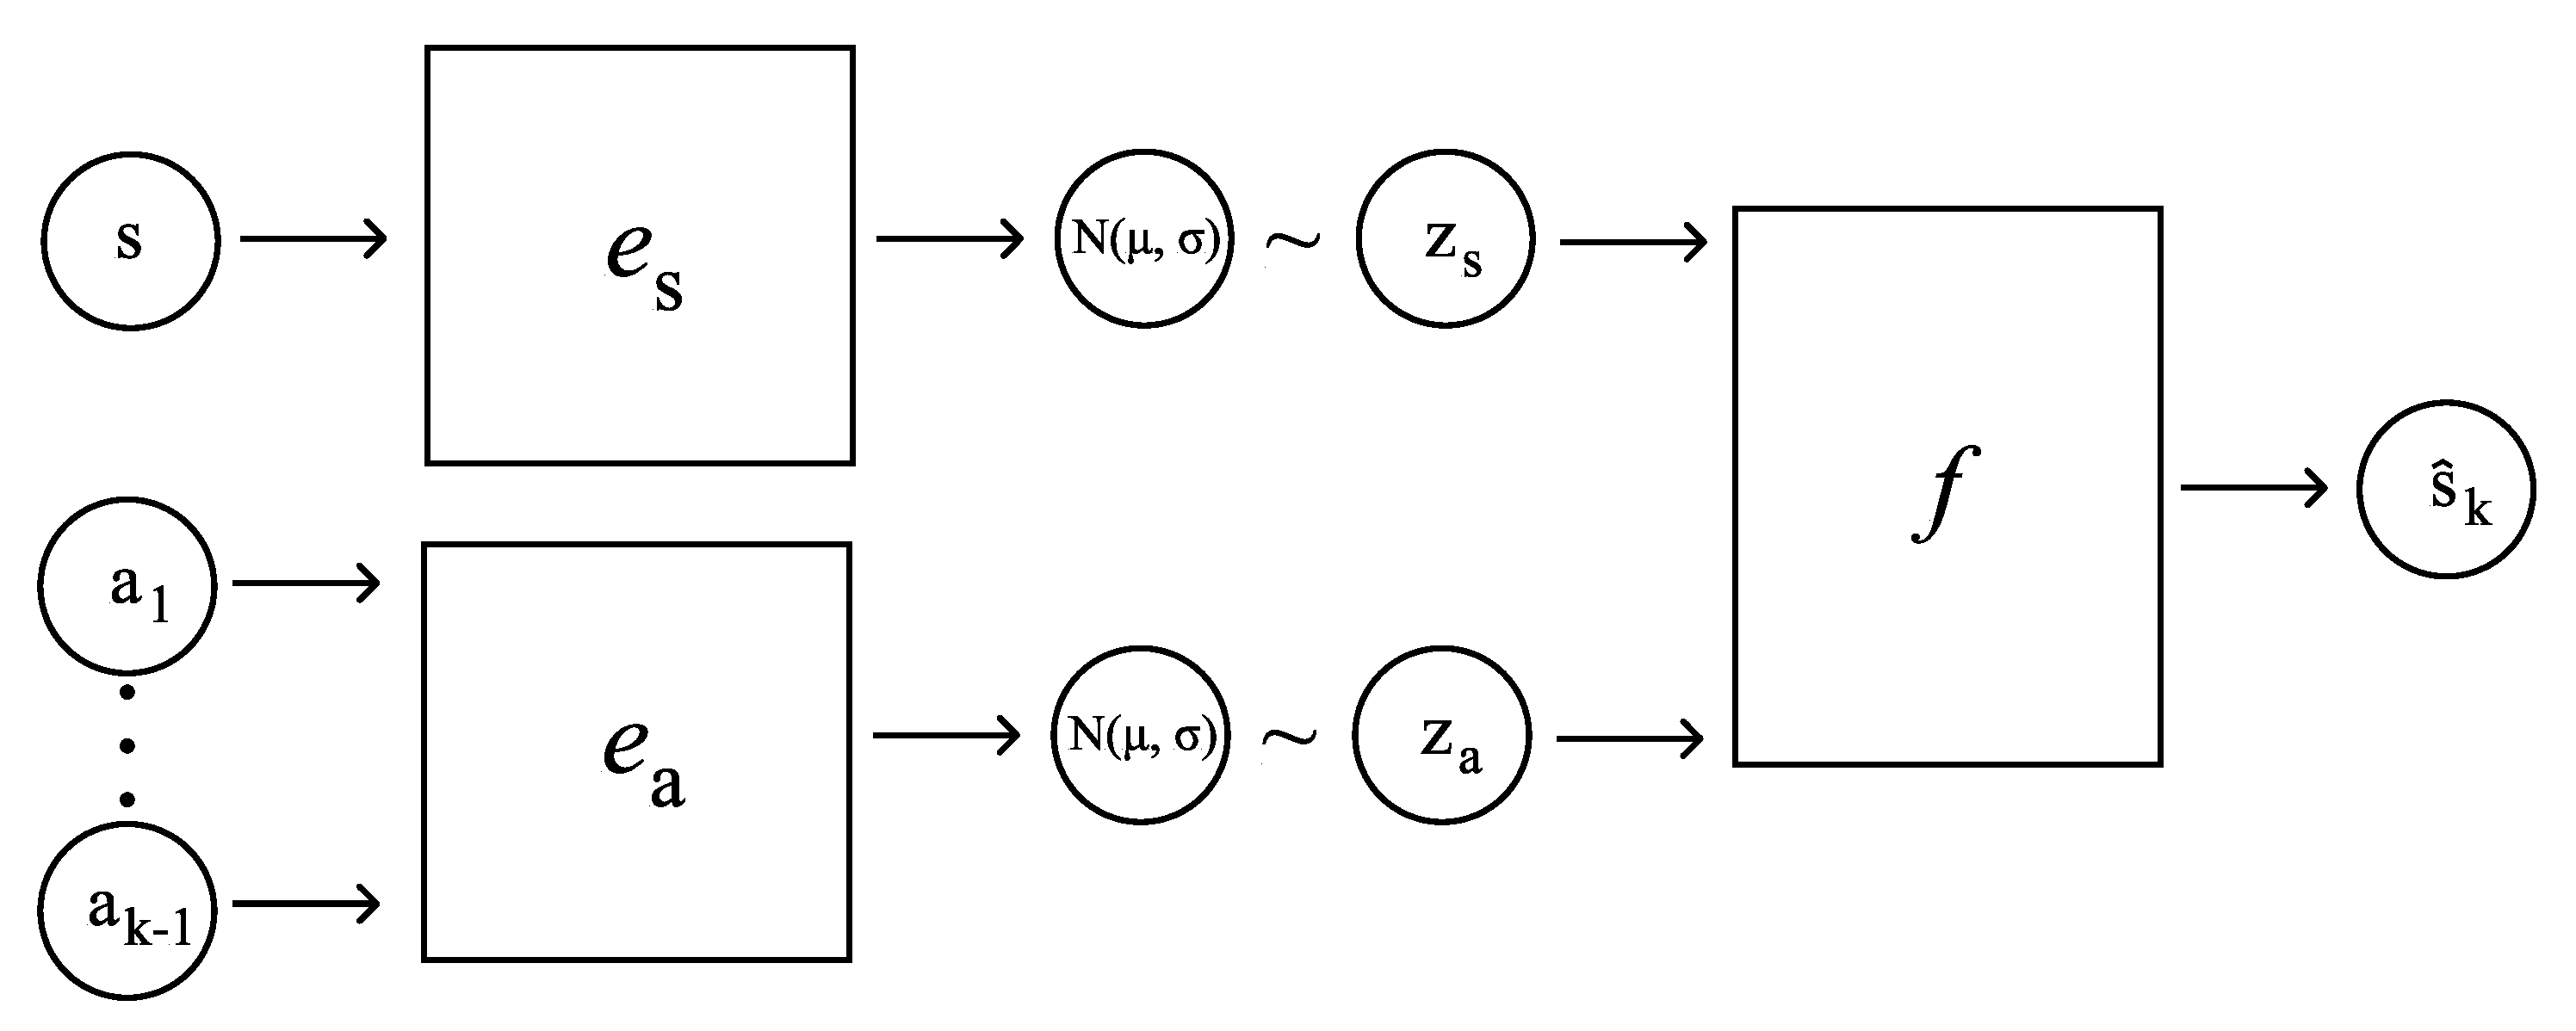
\includegraphics[width=0.7\textwidth]{figures/dyne/model_diagram.pdf}
\centering
\caption{Computational architecture for training the DynE encoders $e_a$ and $e_s$. The encoders are trained to minimize the information content of the learned embeddings while still allowing the predictor $f$ to make accurate predictions.}
\label{fig:model}
\end{figure}

We propose that a good representation for reinforcement learning should represent states or actions close together if they have similar outcomes (resulting trajectories).
This allows the agent to generalize from a small number of samples since each sample accurately reflects the value of all the states or actions in its neighborhood.
In a Markov decision process the outcome of taking an action $a$ in a state $s$ is summarized by the distribution of resulting states $p(s' | s, a) = \trans(s, a)$.
Therefore we construct a method which embeds states and actions such that nearby embeddings have similar distributions of next states.


% be smooth with respect to the optimal value function

% In most practical environments, everything an agent needs to know about a state or an action is captured by its outcome.
% This suggests that any good representation of a state $s$ and an action sequence $\va^k$ should form the sufficient statistics of the distribution of outcomes $p(s' | s, a)$.

Our method, which we call Dynamics-aware Embedding (DynE), learns encoders $e_s$ and $e_a$ which embed a state and action sequence into latent spaces $z_s \in \mathcal{Z}_s$ and $z_a \in \mathcal{Z}_a$ respectively.
These encodings are optimized to form a maximally compressed representation of the sufficient statistics of $p(s' | s, \va^k)$ such that $p(s' | s, \va^k) \approx p(s' | z_s, z_a)$.
% We approximate this objective by maximizing a variational lower bound:
We approximate this by maximizing the following objective:
\begin{align}
\mathcal{L}(\phi_s, \phi_a, \theta) = \E_{s, \va^k, s' \sim \rho^\pi} \Big[ & - \log p(s' | z_s, z_a; \theta)    && \text{predict } s' \label{eq:logprob} \\
 &+ \beta \KL{e_s(s; \phi_s)}{\mathcal{N}(0, \mI)}      && \text{compress } s  \label{eq:skl} \\
 &+ \gamma \KL{e_a(\va^k; \phi_a)}{\mathcal{N}(0, \mI)} \Big]       && \text{compress } \va^k  \label{eq:akl}
\end{align}
where $z_s \sim e_s(s)$, $z_a \sim e_a(\va^k)$, and $\rho^\pi$ is the distribution of transitions under a behavior policy $\pi$.

The DynE objective is similar to a $\beta$-VAE \citep{higgins2017beta} for $s'$ but with a different variational family; like a $\beta$-VAE, it forms a variational lower bound on $p(s')$ when $\beta = \gamma = 1$.
Where a variational autoencoder \citep{kingma2013auto,rezende2014stochastic} or $\beta$-VAE chooses the variational family to be $\mathcal{Q} = \{q(z | s')\}$, we use a factored latent space $\{ z_s, z_a \}$ and independent posterior approximations given the previous state and the action: $\mathcal{Q} = \{ (q(z_s | s), q(z_a | \va^k)) \}$.
This factorization yields separate encoders for states and actions where the state encoder's output is valid for any action and vice versa.
% Like a $\beta$-VAE, when

% Two encoded states $s$ and $\tilde{s}$ should therefore only be close together if the outcome distributions $\trans(s, a)$ and $\trans(\tilde{s}, a)$ are similar for any $a$.

The DynE objective can also be interpreted in the information bottleneck (IB) framework \citep{tishby2000information}.
In the IB framework term \labelcref{eq:logprob} is the prediction objective and terms \labelcref{eq:skl,eq:akl} regularize the latent representation to remove all extraneous information.
Our construction is nearly identical to the approximate information bottleneck proposed by \citet{alemi2016deep}, with the main difference being the factorization of the representation into separate state and action components.

In our experiments we use an isotropic Normal distribution for $p(s' | z_s, z_a; \theta)$ such that term \labelcref{eq:logprob} reduces to $\norm{f(z_s, z_a; \theta) - s'}_2^2$ where $f$ computes the mean.
% This can be interpreted as learning a generative model for $s'$: $z_s, z_a \sim \mathcal{N}(0, \mI)$, $s' \sim \mathcal{N}(f(z_s, z_a), \sigma^2)$ with a fixed $\sigma^2$.
We use diagonal-covariance Normal distributions for $e_s$ and $e_a$ such that $\{\mu_s, \sigma_s^2\} = e_s(s)$, $\{\mu_a, \sigma_a^2\} = e_a(\va^k)$, $z_s \sim \mathcal{N}(\mu_s, \sigma_s^2)$, and $z_a \sim \mathcal{N}(\mu_a, \sigma_a^2)$.
The behavior policy we use for data collection is $\pi = Unif(\mathcal{A})$.



\section{Using learned embeddings for reinforcement learning}

\subsection{Decoding to raw actions}

In order to be useful for RL, the abstract action space produced by the encoder must be decodeable to raw actions in the environment.
Since the mapping from action sequences to high-level actions is many-to-one, inverting it is nontrivial.
We simplify this ill-posed problem by defining an objective with a single optimum.

Once the action encoder $e_a$ is fully trained, we hold it fixed and train an action decoder $d_a$ to minimize

\begin{align}
\mathcal{L}(d_a) = \E_{z_a \sim \mathcal{N}(0, \mI)} \Big[ || e_a(d_a(z_a)) - z_a ||_2^2 + \lambda || d_a(z_a) ||_2^2 \Big] \label{eq:decoder}
\end{align}

The first term of this objective ensures that the action decoder $d$ is a one-sided inverse of $e_a$; that is, $e_a(d_a(z_a)) = z_a$ but $d_a(e_a(a_1, \ldots, a_k)) \ne a_1, \ldots, a_k$.
The second term of the loss ensures that $d_a$ is in particular the minimum-norm one-sided inverse of $e_a$ and gives the objective for the output of $d_a$ a single minimum.
% Intuitively, there may be many sequences of actions which (nearly) always have identical results in terms of $\trans(s, \va^k) ~ \forall s$; \Cref{eq:decoder} selects the one which is smoothest and consumes the least energy.
% The minimum-norm inverse, i.e. the inverse which produces the actions with the smallest norm, is desireable as it leads to actions which are smooth and consume less energy.
Out of all the action sequences which have the same outcome, the minimum-norm sequence is desireable as it leads to trajectories which are smooth and consume less energy.
We choose $\lambda$ to be small (e.g. $10^{-2}$) to ensure that the reconstruction criterion dominates the optimization.


% \red{maybe delete this paragraph, or at least tighten it up}

% This action decoder takes only an embedded action as its input, not a state.
% As a result, if there are multiple environments that share similar dynamics, we can use the same decoder even when the task or the state representations may be different.
% The dynamics must be similar in the sense that the same sets of actions map to similar outcomes across all the environments.
% A sequence of actions does not need to have the \emph{same} outcome in environment A as it does in environment B, but if $\va^k_1$ and $\va^k_2$ are equivalent in environment A they should be equivalent in environment B.
% We show in \Cref{fig:lowd_results} that an action decoder trained on one environment generalizes extremely well to related environments.


\subsection{Efficient RL with temporal abstraction}

Once equipped with a decoder which maps from high-level actions to sequences of raw actions, we train a high-level policy that solves a task by selecting high-level actions.
In this section we extend the deterministic policy gradient \citep{silver2014deterministic} family of algorithms to work with temporally-extended actions while maintaining off-policy updates and learning from every environment step.
This allows our method to achieve superior sample efficiency when working with high-level actions.
In particular, we extend the twin delayed deep deterministic policy gradient (TD3) algorithm \citep{fujimoto2018addressing} to work with the DynE representation of actions to form an algorithm we call DynE-TD3.

We first describe why DPG requires modifications to accommodate temporally-abstracted actions. One simple approach to combining DynE with DPG would be to incorporate the $k$-step DynE action space into the environment to form a new MDP.
This MDP allows the use of DPG without modification; however, it only emits observations once every $k$ timesteps.
As a result, after $N$ steps in the original environment, the deterministic policy $\mu$ and critic function $Q$ can only be trained on $N/k$ observations.
This has a substantial impact on sample efficiency when measured in the original environment.

Instead we require an algorithm which can perform updates to the policy $\mu$ and critic $Q$ for every environment step.
To do this, we train both $\mu$ and $Q$ in the abstract action space with minor changes to their updates.
We distinguish these functions which use DynE actions from their raw equivalents by adding a superscript $\text{DynE}$, i.e. $\mu^{\text{DynE}}$ and $Q^{\text{DynE}}$.
We augment the critic function with an additional input, $i$, which represents the number of steps $0 \le i < k$ of the current embedded action $z$ that have already been executed.
This forms the DynE-TD3 critic:

\begin{align}
\label{eq:critic}
Q^{\text{DynE}}(e_s(s_t), z_t, i) = \sum_{j=0}^{k-i-1} \big( \gamma^j r_{t+j} \big) + \gamma^{k-i} Q^{\text{DynE}} \Big( e_s(s_{t+k-i}), \mu^{\text{DynE}}(e_s(s_{t+k-i})), 0 \Big)
\end{align}

In plain language, the value of being on step $i$ of abstract action $e_t$ is the value of finishing the remaining $(k-i)$ steps of $z_t$ and then continuing on following the policy.
This is similar to the idea of $k$-step returns \citep{sutton2018reinforcement}, but with a variable $k$ which depends on the step within the current plan.
Whereas $k$-step returns would typically require an off-policy correction such as Retrace \citep{munos2016safe}, conditioning on $z_t$ and $i$ determines all $k-i$ actions in the return.
In effect, they remain a single action, making the update valid off policy.
The DynE critic is trained by minimizing the Bellman error implied by \cref{eq:critic}.

To update the policy we follow the standard DPG technique of using the gradient of the critic.
We modify the algorithm to take into account that $i=0$ at the time of issuing a new high-level action.
The gradient of the return with respect to the policy parameters is then

\begin{align}
\nabla_\theta J_\pi(\mu^{\text{DynE}}_\theta) \approx \E_{s \sim \rho^\pi} \Big[ \nabla_\theta \mu^{\text{DynE}}_\theta(e_s(s)) ~ \nabla_z Q^{\text{DynE}}(e_s(s), z, 0)|_{z=\mu^{\text{DynE}}_\theta(e_s(s))} \Big]
\end{align}

given that data was collected according to a behavior policy $\pi$.


\section{Related work}
Successor representations, an inspiration for this work, represent a state by the expected rate of future visits to other states \citep{dayan1993improving,kulkarni2016deep,barreto2017successor}.
Successor representations have been demonstrated to be an effective model of animal and human learning \citep{momennejad2017successor,stachenfeld2017hippocampus}.
They are also one of the earliest realizations of the idea of representing each state by its future.
Whereas successor representations learn future occupancy maps for a particular policy, we learn an embedding space where states are close together if they have similar outcomes for any policy.

Several papers have proposed using (variational) auto-encoders to learn embeddings for observations \citep{lange2010deep,van2016stable,higgins2017darla,caselles2018continual}; unlike our work, these models operate on a single observation at a time and do not depend on the environment dynamics.
Forward prediction has also been used as an auxiliary task to speed RL training \citep{jaderberg2016reinforcement}, and \citet{Jonschkowski2017PVEsPE} learn representations which adhere to physical constraints.
\citet{ghosh2018learning} propose to learn state embeddings using the action distribution of a goal-conditioned policy; however, their technique depends on already having a successful policy.
Other work has proposed to use mutual information maximization to learn embeddings which facilitate exploration via intrinsic motivation \citep{kim2018emi}.

% Another line of work couples the process of learning a model of the environment with training a policy on imagined rollouts \citep{sutton1991dyna,deisenroth2011pilco,ha2018world,clavera2018model,kaiser2019model,henaff2019model}.These works are similar to ours in that they learn forward models of the environment and use them to speed the training of model-free policies.
% However, our work differs from theirs in that we use forward modeling only as a surrogate objective for representation learning.

Similarly to this work, hierarchical reinforcement learning seeks to learn temporal abstractions.
These abstractions are variously defined as skills \citep{florensa2017stochastic, hausman2018learning}, options \citep{sutton1999between, bacon2017option}, or goal-directed sub-policies \citep{kulkarni2016hierarchical, vezhnevets2017feudal}.
% Whereas these works train a low-level policy by maximizing the reward of the overall task or a heuristically-defined subtask, in this work we seek to learn a representation of the transition structure of the environment which can be used for any downstream task.
Most closely related are SeCTAR \citep{CoReyes2018SelfConsistentTA} and HIRO \citep{Nachum2018NearOptimalRL}.
SeCTAR simultaneously learns a generative model of future states and a low-level policy which can reach those states.
% Unlike this work, their latent space represents a particular trajectory through the environment rather than an outcome, making it state-dependent.
% Furthermore, SeCTAR assumes the reward function is given ahead of time.
HIRO learns a representation of goals such that a high-level policy can induce any action in a low-level policy.
% However, their off-policy performance depends on an approximate re-labeling of action sequences to train the high-level policy.
Unlike this work, both SeCTAR and HIRO learn state-dependent low-level policies, not action representations.
Furthermore SeCTAR assumes the reward function is given ahead of time, and HIRO's off-policy performance depends on an approximate re-labeling of action sequences to train the high-level policy.
% A follow-up paper \citep{Nachum2018NearOptimalRL} learns a representation for goal states such that a high-level policy can induce any action in a low-level policy.

Also related are methods which attempt to learn embeddings of single actions to enable efficient learning in very large action spaces \citep{dulac2015deep, chandak2019learning}.
In particular, \citet{chandak2019learning} learns a latent space of actions based on the effects of an action on the environment. However, their latent spaces are for a single action and they do not consider learned state representations.
Another related direction is learning embeddings of one or more actions from demonstrations \citep{tennenholtz2019natural}; this embedded action space builds in prior knowledge from the demonstrator and can allow faster learning.



\section{Representation Experiments}

% In this section we empirically investigate the properties of the learned DynE representations and their relationship with the environment dynamics.
% We first visualize the relationship between DynE actions and their effects in the environment, then show how this tight coupling between actions and multi-step outcomes can improve exploration.
In this section we empirically investigate how the learned DynE representations reshape the problem of reinforcement learning.
First we make a connection between temporal abstraction and exploration, revealing that DynE actions result in better state coverage.
Then we probe the relationship between DynE state embeddings and the task value function.
% \red{change if I use a state plot}


% \subsection{Visualizing the DynE action space}
% \label{sec:latent-vis}

% \red{replace this figure with one about states or clean it up}

% To better understand the structure in the DynE action embedding space, we visualize the relationship between the outcome of a sequence of actions and the DynE embedding of those actions.
% In particular, when embedding an action sequence, the DynE objective seeks to preserve information about the outcome of that action sequence (i.e. the change in state), but minimize information about the original action sequence.
% Therefore we should see that all action sequences which have similar outcomes embed close together, regardless of the actions along the way.
% We investigate this by plotting the 2D DynE embedding of 10K action sequences and coloring them by their outcome under the environment dynamics.
% If the DynE embedding depends on the actions within the sequence and not just the outcome, some sequences with similar outcomes (colors) will be embedded far apart.
% \Cref{fig:spaces} shows the result of this experiment in a simple Point environment with an easy-to-visualize 2D $(x, y)$ state.
% For this simple problem, we see that all pairs of action sequences $\va^k_1$ and $\va^k_2$ with similar outcomes are close together in the embedding space.
% % The correspondence between the two spaces appears to remain strong for high-dimensional and nonlinear environments, but is much harder to render in two dimensions.

% \begin{figure}[h]
% \centering
% \begin{subfigure}[t]{0.35\textwidth}
%     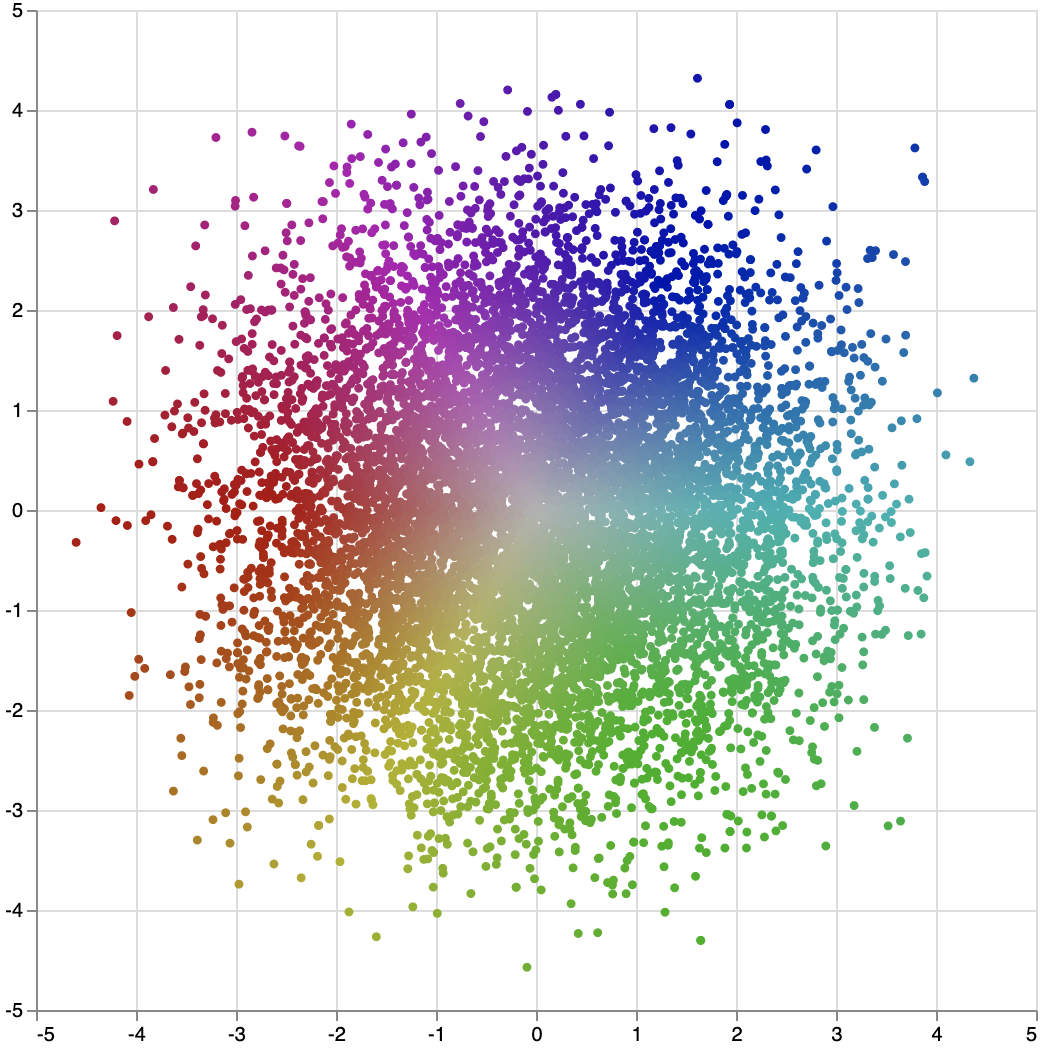
\includegraphics[width=\textwidth]{figures/dyne/state_space_rainbow.png}
%     \caption{Outcome space}
% \end{subfigure}
% \begin{subfigure}[t]{0.35\textwidth}
%     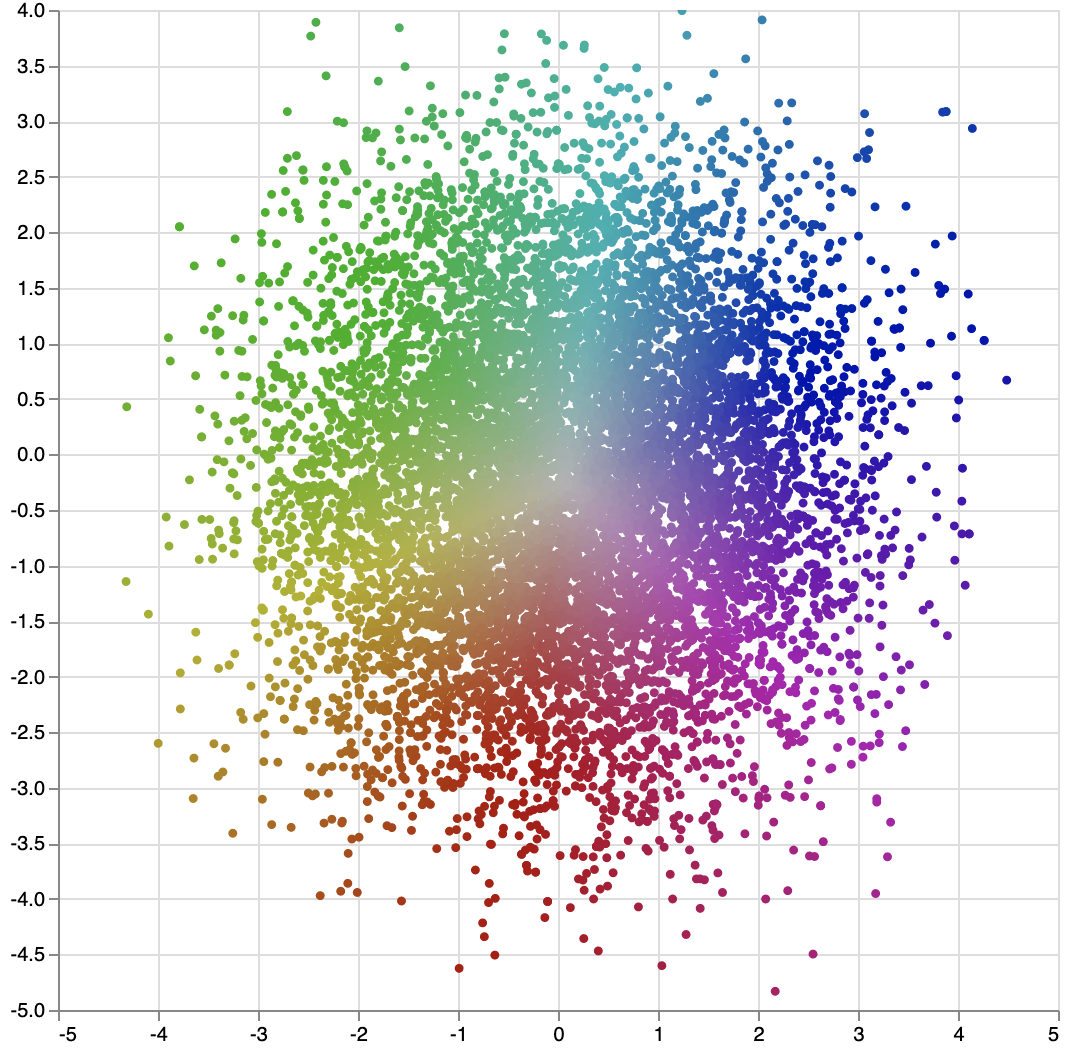
\includegraphics[width=\textwidth]{figures/dyne/latent_space_rainbow.png}
%     \caption{DynE action space}
% \end{subfigure}
% \caption{The mapping between the outcomes and embeddings of action sequences.
% We sample 10K random sequences of four actions and evaluate their outcomes in the environment dynamics, measured by $(\Delta x, \Delta y) = s_{t+4} - s_t$.
% \textbf{(a)} We plot the outcome $(\Delta x, \Delta y)$ of each action sequence and color each point according to its location in the plot.
% \textbf{(b)} We use DynE to embed each action sequence into two dimensions; each point in this plot corresponds to a point in (a) and takes its color from that corresponding point.
% The similarity of the two plots and the smooth color gradient in (b) indicate that DynE is embedding action sequences according to their outcomes.
% }
% \label{fig:spaces}
% \end{figure}

\subsection{Temporal abstraction and exploration}


% \red{rewrite to explain why temporal abstraction helps exploration}


When embedding an action sequence, the DynE objective seeks to preserve information about the outcome of that action sequence (i.e. the change in state), but minimize information about the original action sequence.
% Therefore we expect all action sequences which have similar outcomes to embed close together, regardless of the actions along the way.
% Appendix \ref{sec:latent-vis} empirically verifies this property in a simple environment.
As shown in Appendix \ref{sec:latent-vis}, this leads to a representation where all action sequences which have similar outcomes embed close together.
% This has benefits for exploration.
% Uniformly selecting a raw action at every timestep leads to over-sampling the area around the starting position.
% If uniformly selecting an abstract DynE action of length $k$ results in reaching a state uniformly sampled from the $k$-step ball around the starting point,
We propose that this temporally abstract action space, where actions correspond to multi-step outcomes, allows random actions to explore the environment more efficiently.

We empirically validate the exploration benefits of the temporally abstract DynE actions.
\Cref{fig:exploration_histogram} shows that uniformly sampling a DynE action results in a nearly uniform distribution over the states reachable within $k$ steps.
Over the course of an entire episode, selecting DynE actions uniformly at random reaches faraway states more often than random exploration with raw actions.
% We also provide a visualization of the learned DynE action space in Appendix \ref{sec:latent-vis}
Appendix \ref{sec:exploration_trajs} shows the qualitative difference between random trajectories in the raw and DynE action spaces, and Appendix \ref{sec:varying_k} studies the impact of varying $k$ on the performance of a learned policy.

\begin{figure}[h]
\centering
    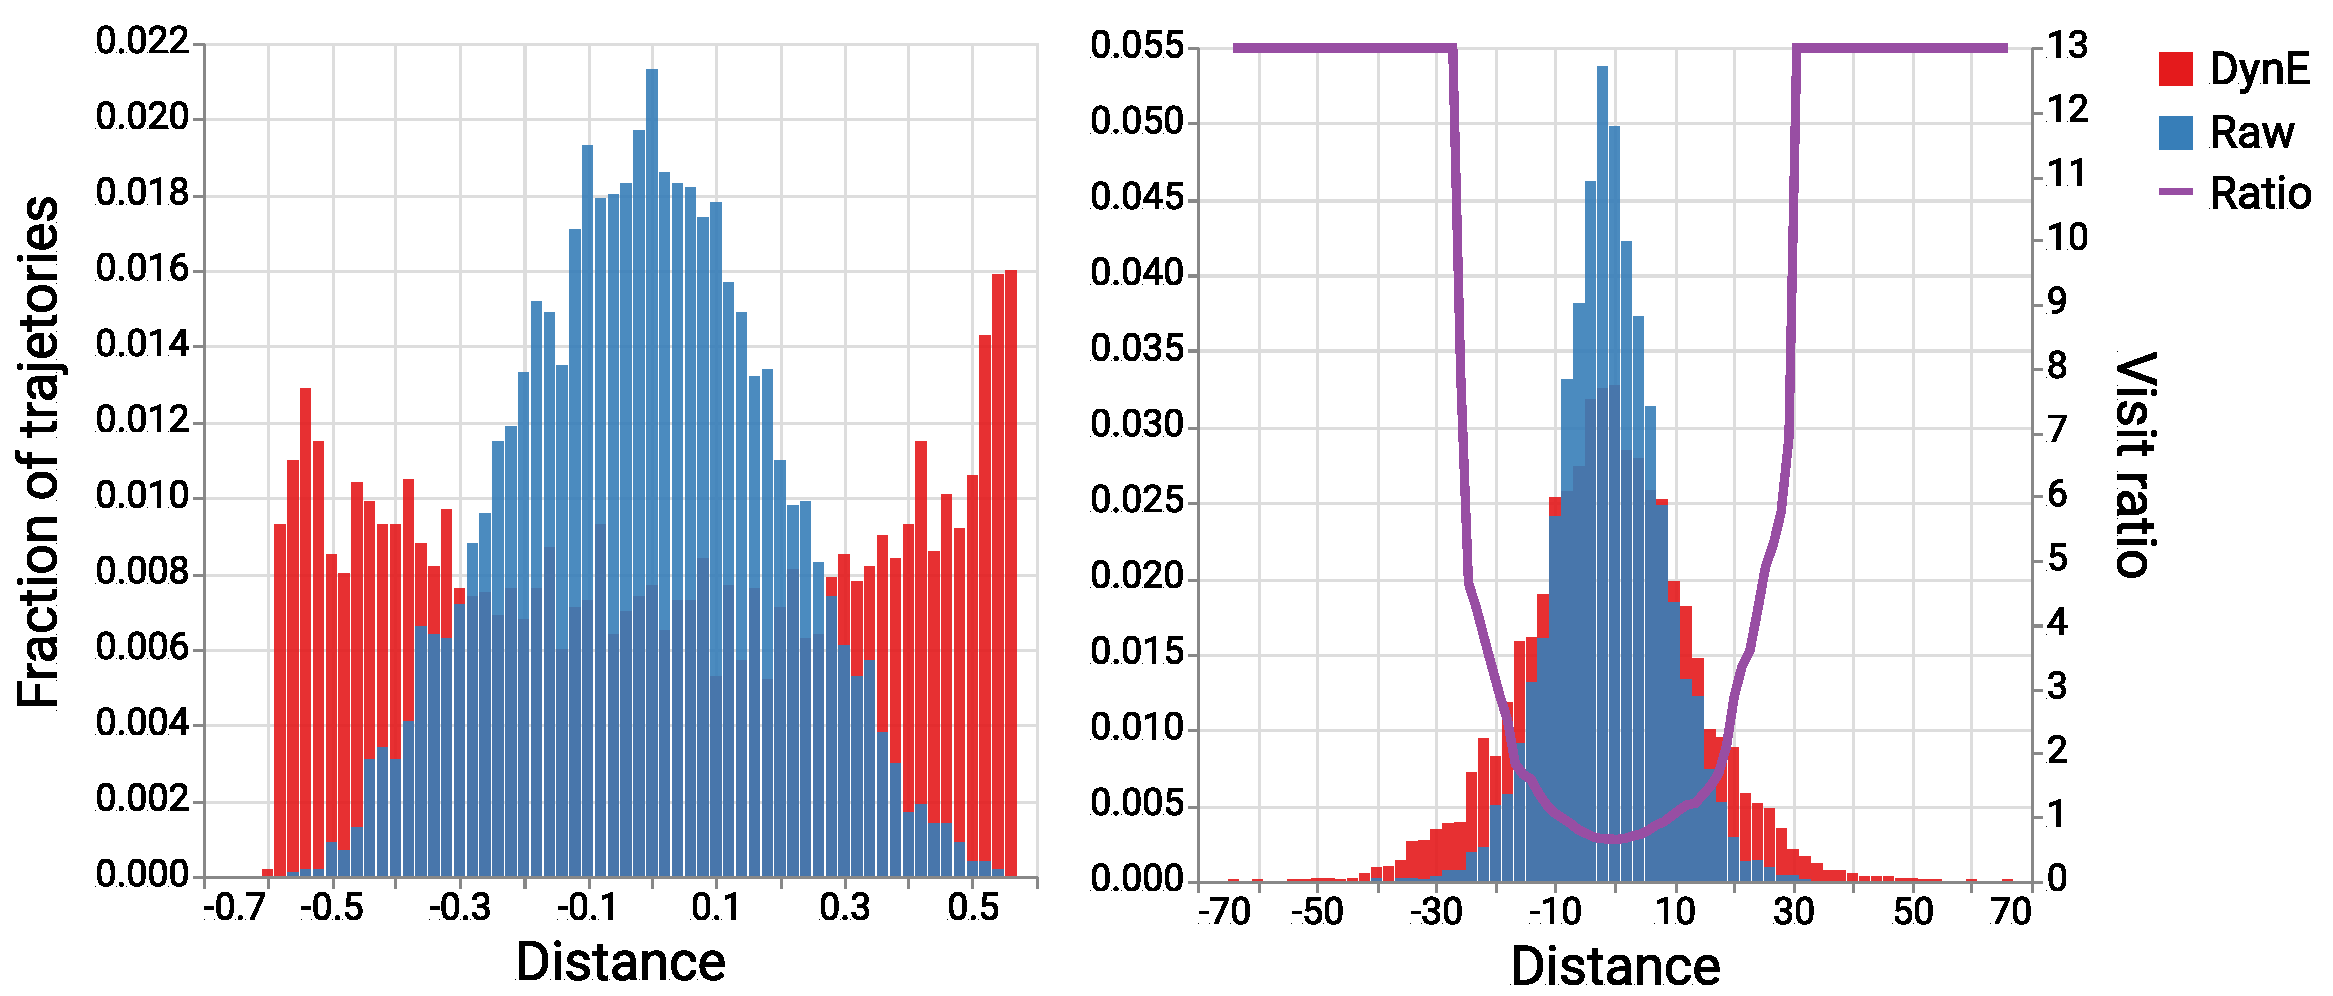
\includegraphics[width=0.7\textwidth]{figures/dyne/exploration_histograms_ratio_sidelegend.pdf}
\caption{The distribution of state distances reached by uniform random exploration using DynE actions ($k=4$) or raw actions in Reacher Vertical. \textbf{Left:} Randomly selecting a 4-step DynE action reaches a state uniformly sampled from those reachable in 4 environment timesteps. \textbf{Right:} Over the length of an episode (100 steps), random exploration with DynE actions reaches faraway states very much more often than exploration with raw actions. The visit ratio shows how frequently DynE exploration reaches a certain distance compared to raw exploration.}
\label{fig:exploration_histogram}
\end{figure}

\subsection{State representations}

The DynE objective compresses states while preserving information about the outcome of taking any action in that state.
If this compression is successful, states which have similar outcomes will be close together in embedding space.
In an MDP, two states which have identical successor states have values which differ by at most the range of the reward function $r_{\max} - r_{\min}$.
While in general states which lead to merely similar successors may have arbitrarily different value, we suggest that in many tasks of interest, similar successors may entail similar value.

We investigate whether the DynE state embedding leads to neighborhoods with similar value in the Reacher Vertical environment.
We collect 10K states from a random policy in the environment and perform dimensionality reduction on three representations of those states: the DynE embedding of state images, low-dimensional joint states, and pixels.
\Cref{fig:state_tsne} shows the results of this dimensionality reduction, in which every point is colored by its value under a fully-trained TD3 policy on the low-d states.
DynE embeddings have neighborhoods with more similar values than states or pixels.

\begin{figure}[h]
\vspace{-0.5em}
\centering
    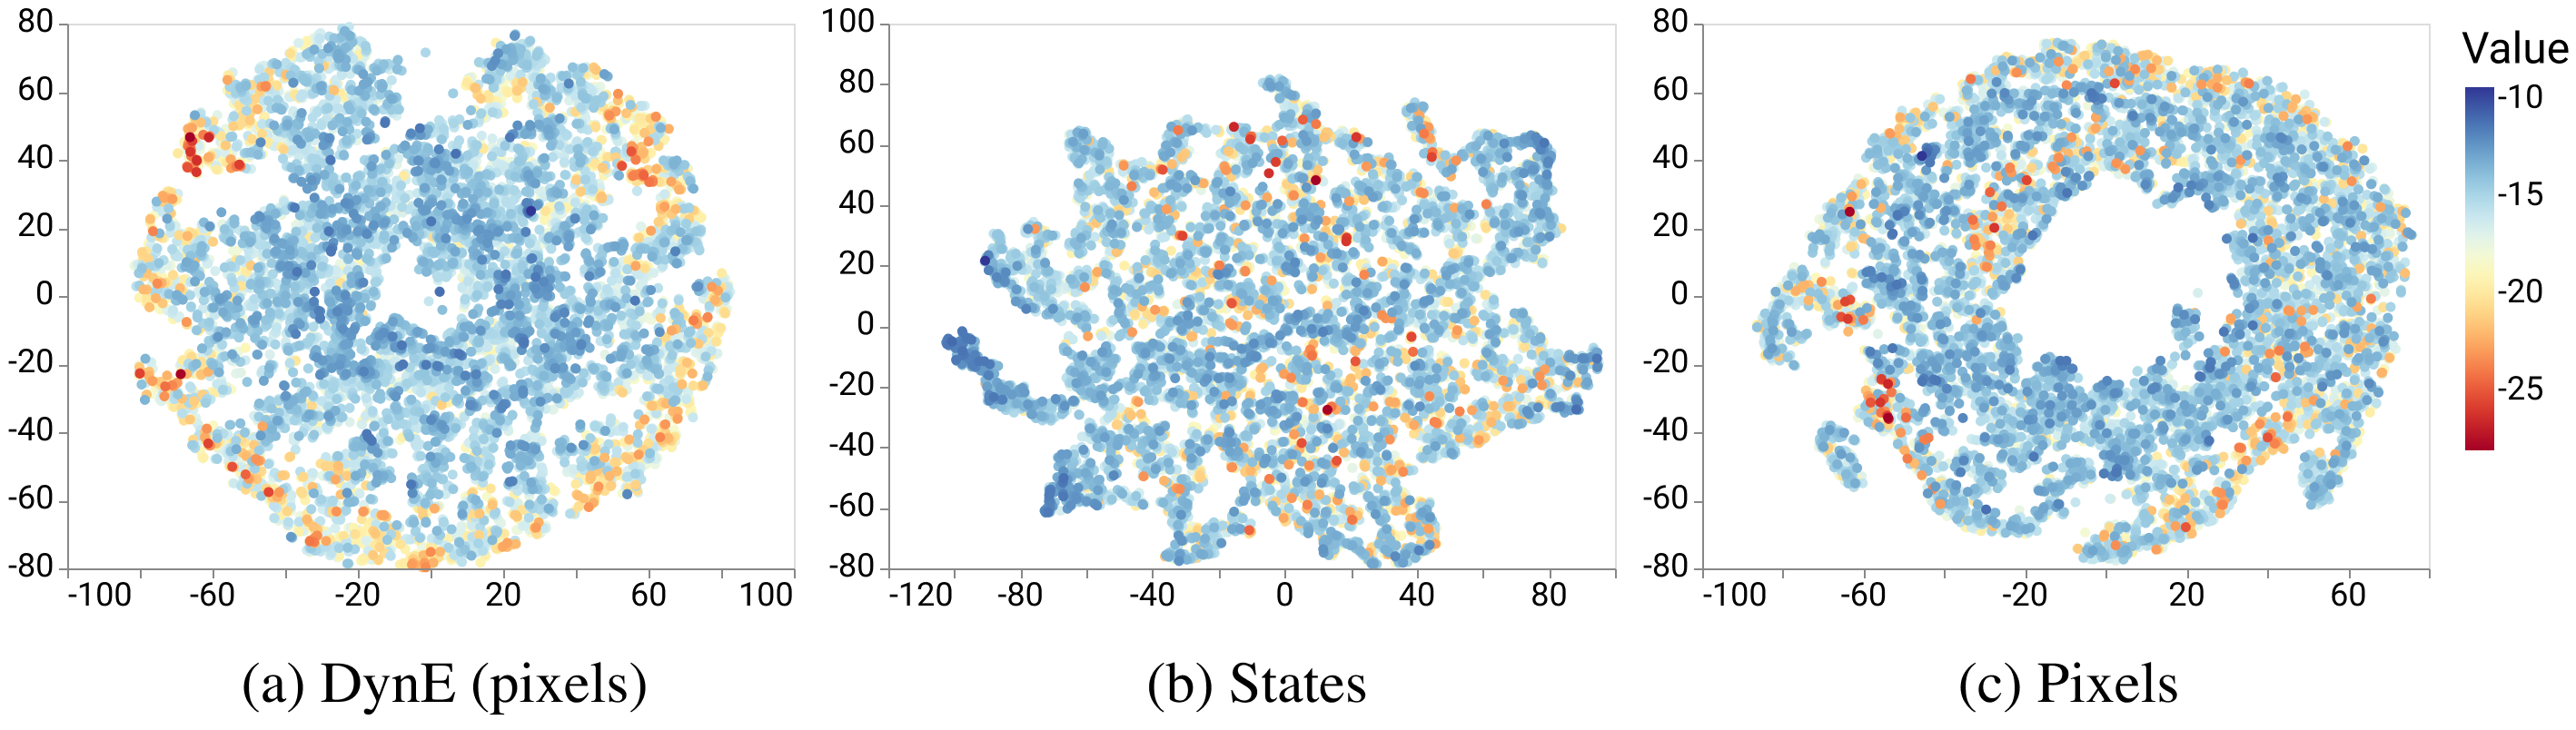
\includegraphics[width=0.99\textwidth]{figures/dyne/state_tsne.png}
\caption{The relationship between state representations and task value. Each plot shows the t-SNE dimensionality reduction of a state representation, where each point is colored by its value under a near-optimal policy.
(a) The DynE embedding from pixels places states with similar values close together.
(b) The low-dimensional states, which consist of joint angles, relative positions, and velocities, have some neighborhoods of similar value, but also many regions of mixed value.
(c) The relationship between the pixel representation and the task value is very complex.
% (b) and (c) The low-dimensional states, which consist of angles and velocities, have some neighborhoods of similar value, but also many isolated points.
% (c) The relationship between the pixel representation and the task value is very complex.
}
\label{fig:state_tsne}
\end{figure}

% We provide a similar investigation of the relationship between DynE's action embeddings and their outcomes in the environment in Appendix \ref{sec:latent-vis}, which shows that DynE actions have a one-to-one correspondence with outcome states.

\section{Reinforcement learning experiments}
%  and their effectiveness for deep RL
In this section we assess the effectiveness of the DynE representations for deep RL, individually analyzing the contributions of the action and state representations before combining them.
% we separately analyze the contributions of the learned action and state representations.
First we evaluate the DynE action space on a set of six tasks with low-dimensional state observations, testing its usefulness across a set of tasks and object interactions.
% including transferring the learned action space between environments with similar dynamics but different tasks and objects.
Then, we test the DynE state space on a set of three tasks with pixel observations.
Finally, we combine DynE actions with DynE observations, verifying that the two learned representations are complementary.

Appendix \ref{sec:hyperparams} provides a full description of hyperparameters and model architectures, and all of the code for DynE is available on GitHub at \url{https://github.com/dyne-submission/dynamics-aware-embeddings}.

\paragraph{Environments}

We use six continuous control tasks from two families implemented in the MuJoCo simulator \citep{todorov2012mujoco} to evaluate our method.
Within each family, the task and observation space change but the robot being controlled stays roughly the same, allowing us to test the transferrability of the DynE action space between tasks.
The Reacher family consists of three of tasks which involve controlling a 2D, 2DoF arm to interact with various objects.
The 7DoF family of tasks from OpenAI Gym \citep{brockman2016openai} is quite difficult, featuring three tasks in which a 3D, 7DoF arm must use different end effectors to push or throw various objects to randomly-generated goal positions.
Images and detailed descriptions of both families of tasks are available in Appendix \ref{sec:task-renders}.


\subsection{Low-dimensional states}
\label{sec:action_experiments}


% We use both families of tasks to evaluate the performance of the DynE action space and its generality across tasks.
% Whereas directly transferring a policy to an environment with different objects and observations would be impossible, DynE actions .

For training the DynE action representation we use 100K steps with a uniformly random behavior policy in the simplest environment in each family with no reward or other supervisory signal.
As this DynE pretraining is unsupervised and only occurs once for each family of environments, the $x$ axis on these training curves refers only to the samples used to train the policy.\endnote{On all environments except the simplest (Reacher Vertical) shifting the DynE-TD3 plot by 100K steps does not affect the ordering of the results.}
We then transfer this action representation to all three environments in the family.
When training DynE-TD3 we use all of the default hyperparameters from the TD3 implementation across all environments.

We directly test the impact of switching from raw to DynE actions by comparing TD3 to DynE-TD3.
For completeness we compare with two additional state-of-the-art model-free methods: soft actor-critic (SAC) \citep{haarnoja2018soft,haarnoja2018softapp} and proximal policy optimization (PPO) \citep{schulman2017proximal}.
We also compare with soft actor-critic with latent space policies (SAC-LSP) \citep{haarnoja2018latent}, an innovative hierarchical method which transforms a low-level action space into an abstract one by training an invertible low-level policy.
In all cases we use the official implementations\endnote{TD3: \url{https://github.com/sfujim/TD3/}}\endnote{SAC and SAC-LSP: \url{https://github.com/haarnoja/sac}}\endnote{PPO: \url{https://github.com/openai/baselines/tree/master/baselines/ppo2}}
and the MuJoCo hyperparameters used by the authors.
We also attempted to compare with the hierarchical method by \citet{Nachum2018NearOptimalRL}, but after several emails with the authors and dozens of experiments we were unable to get it to converge on tasks other than those in their paper.

\paragraph{Results}
\Cref{fig:lowd_results} shows the results of these experiments.
Most significantly, they show that switching from the raw action space (TD3 curve) to the DynE action space results in faster training and allows TD3 to solve the difficult 7DoF suite of tasks.
We see that the DynE action space generalizes across several tasks with the same robot, even when interacting with objects unseen during training.
% They show that (1) high-quality policies can be trained on the DynE action space; (2) TD3 shows substantial efficiency gain from using the DynE action space; and (3) the DynE space generalizes across several tasks with the same robot, even when interacting with objects unseen during training.
It is especially worth noting that the gains from DynE increase as the tasks become harder, maintaining convergence, stability, and low variance in the face of high-dimensional control with difficult exploration.
Since SAC-LSP \citep{haarnoja2018latent} performs similarly but worse than SAC we test it only on the simpler Reacher family of tasks; meanwhile, the PPO curves do not enter the frame on the Reacher family of tasks due to its poor sample efficiency.

\begin{figure}[t]
\centering
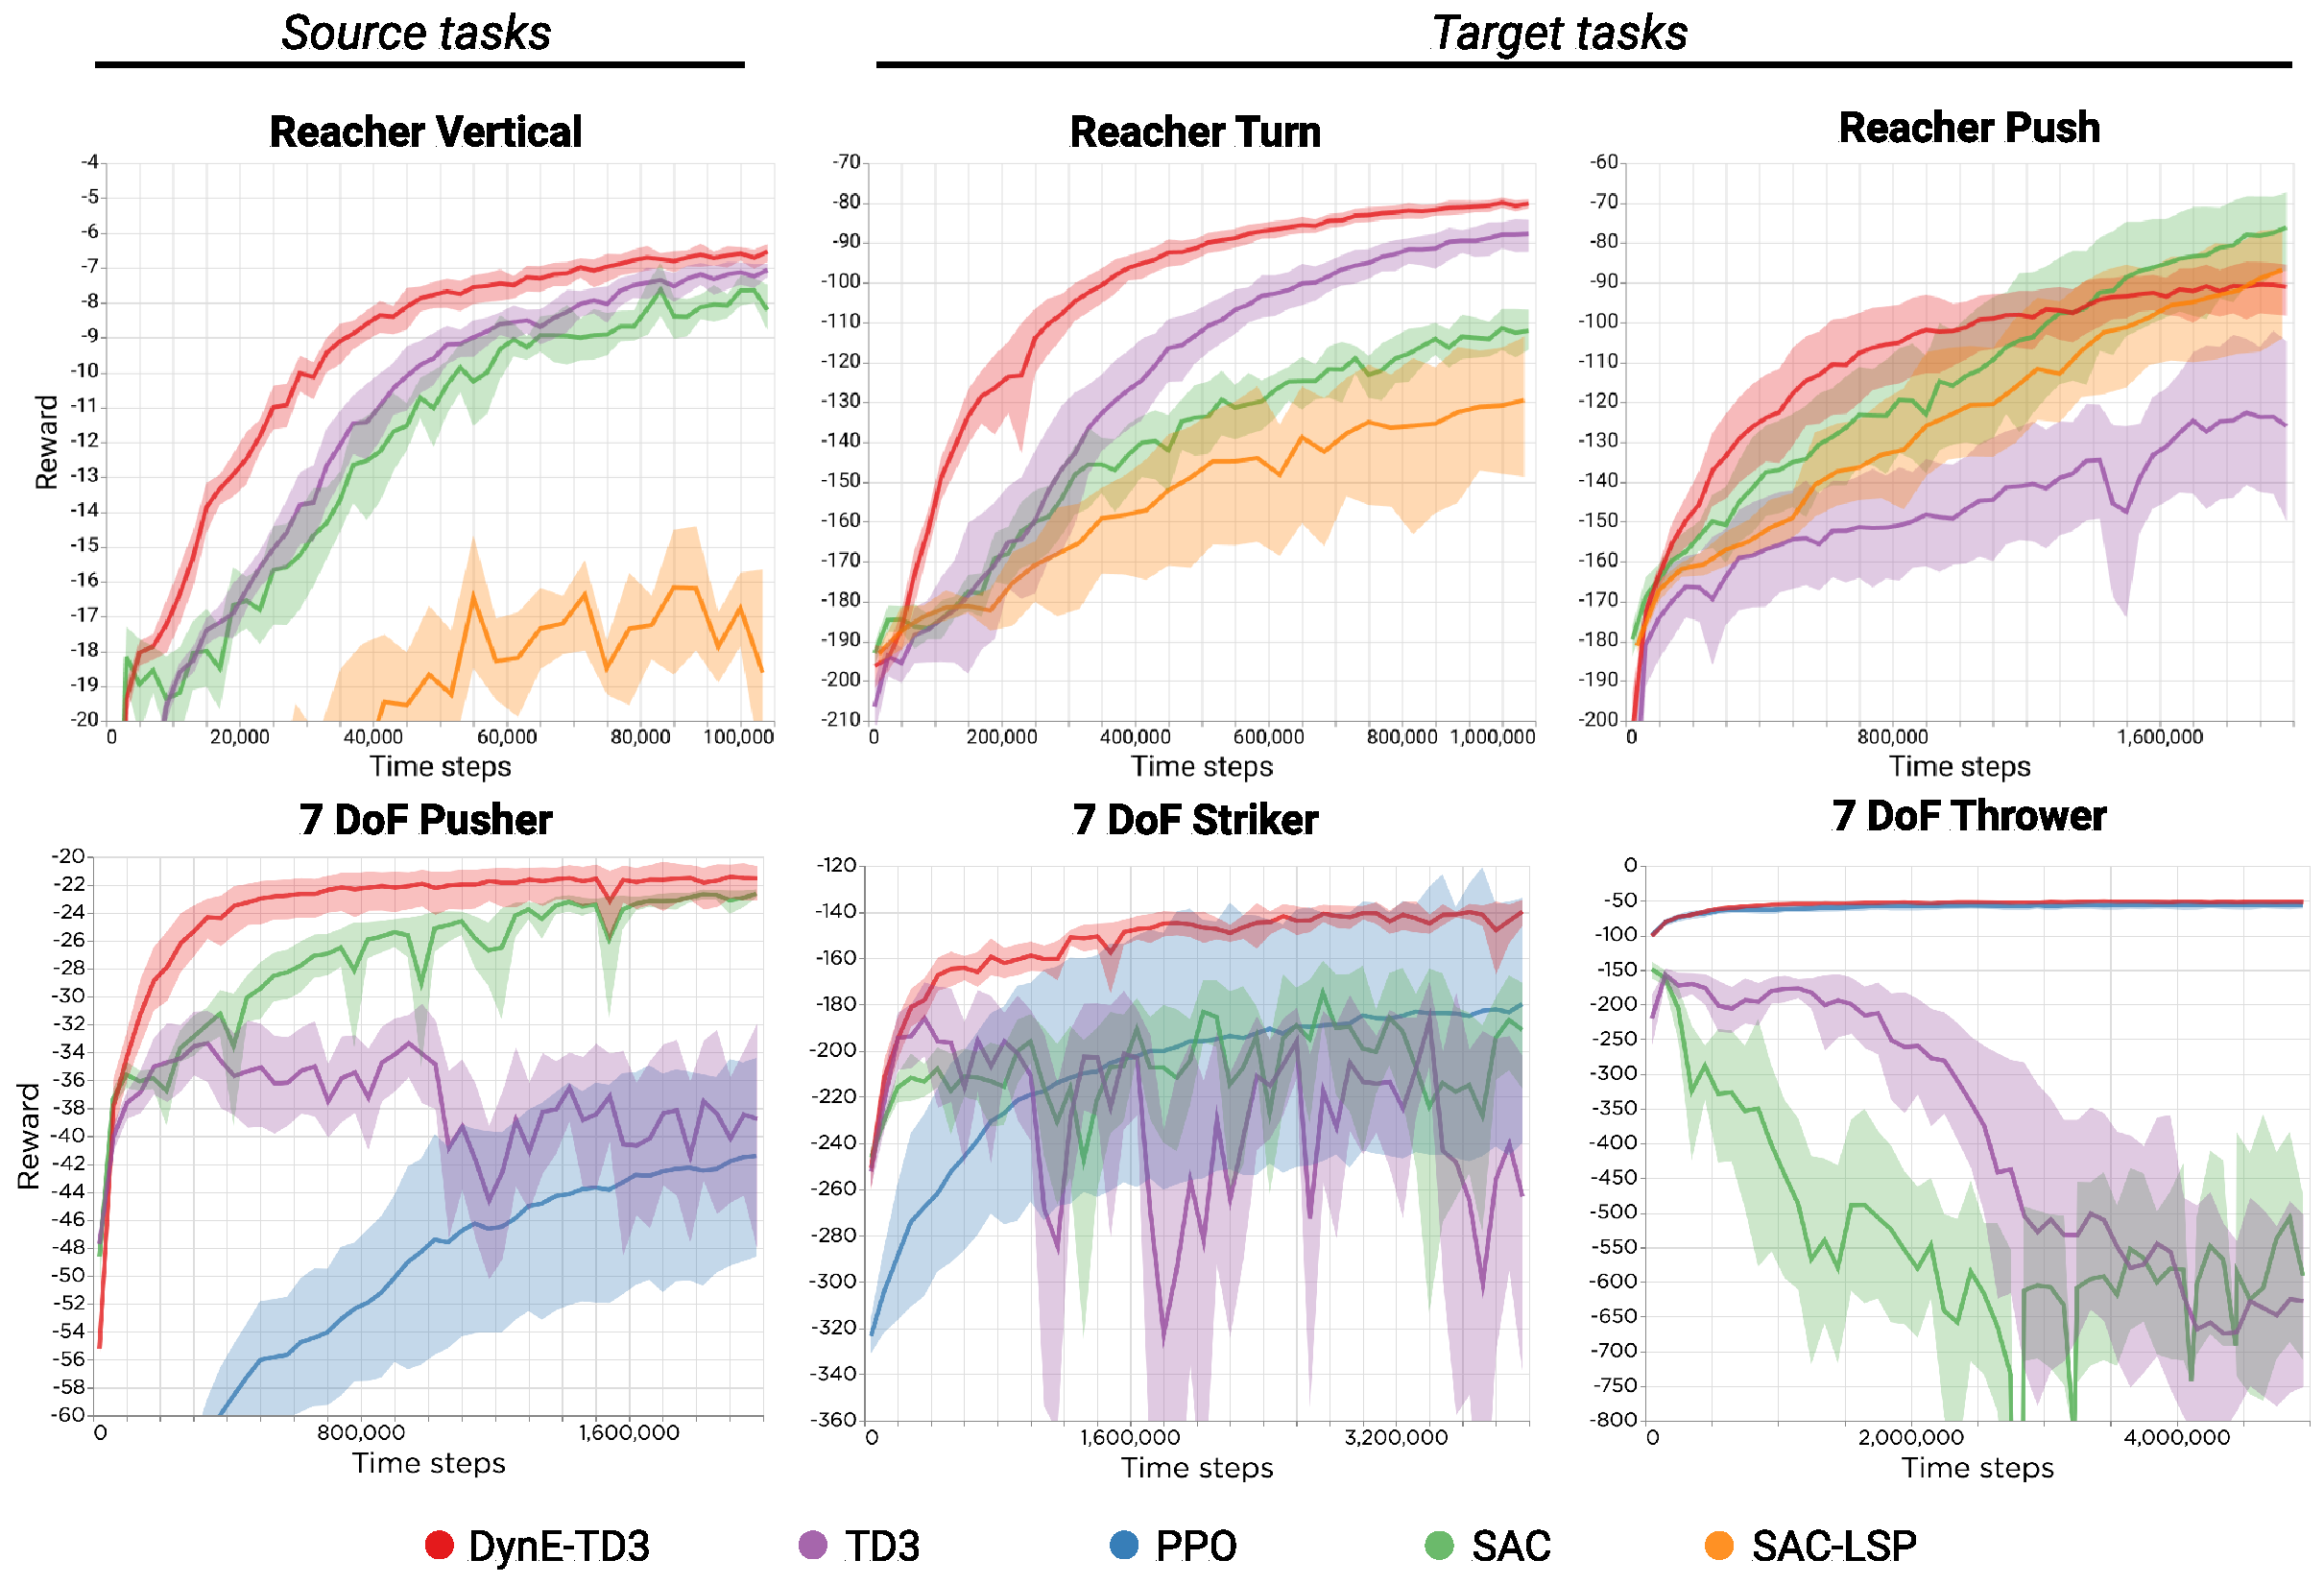
\includegraphics[width=0.9\textwidth]{figures/dyne/states_results_lsp_smalltitle.pdf}
\caption{Performance of DynE-TD3 and baselines on two families of environments with low-dimensional observations.
Dark lines are mean reward over 8 seeds and shaded areas are bootstrapped 95\% confidence intervals.
Across all the environments, TD3 learns faster with the DynE action space than with the raw actions.
Within each family of environments, the DynE action space was trained only on the simplest task (left).}
\label{fig:lowd_results}
\end{figure}

\subsection{Pixels}

% \red{talk about DARLA and why it's a good comparison}

Using the Reacher family of environments we evaluate several state representations by their effectiveness for policy learning with TD3.
% To train the DynE state space we use 100K steps from a uniformly random policy in each environment; since the DynE state representation must be trained on each environment, we include those 100K steps in the $x$ axis of our training curves.

We evaluate two established methods for learning representations from single images.
``DARLA'' is the Disentangled Representation Learning Agent proposed by \citet{higgins2017darla} with the denoising autoencoder loss, which is referred to in that work as $\beta$-VAE$_{DAE}$.
``VAE'' is a standard variational autoencoder \citep{kingma2013auto,rezende2014stochastic}, which has previously been found to learn effective representations for control \citep{van2016stable}; it is equivalent to DARLA with the pixel-space loss and $\beta=1$.
% To enable direct comparison we train both state representation baselines on the same dataset we use for DynE, then use their encoding as the state space for TD3.
Since these representations operate on a single frame at a time, we apply them to the most recent four frames independently and then concatenate the embeddings before feeding them to the policy.
These representations have compressed latent spaces, but they encode no knowledge of the environment's dynamics, allowing us to evaluate the importance of incorporating the dynamics into our embeddings.

Next we evaluate representation learning methods whose objectives incorporate the dynamics.
``S-DynE,'' for State DynE, is the DynE state embedding $e_s$, and ``SA-DynE'' combines the DynE state and action representations.
``S-Deterministic'' and ``SA-Deterministic'' are ablations of the corresponding DynE methods which have the same forward-prediction objective but no KL or noise on the latent representations.
Comparing the DynE methods to their respective ablations reveals the contribution of explicitly introducing a compression objective to the latent space.

% Finally, we evaluate whether using a learned action space in combination with the learned state space yields additional gains.
% We label the policies trained with both state and action DynE representations ``SA-DynE''.
% ``SA-Deterministic'' is an ablation of SA-DynE with no KL or noise in either the state or action latent spaces.
For training all of the learned representations we use a dataset of 100K steps in each environment from a uniformly random policy.
In every case we train TD3 with the learned representations using all of the default hyperparameters from the official TD3 implementation.

% Next we evaluate two state representation learning methods whose objectives incorporate the dynamics.
% ``S-DynE,'' for State DynE, is the DynE state embedding $e_s$.
% ``S-Deterministic'' is an ablation of S-DynE which has the same forward-prediction objective but with no KL or noise on the latent representation.
% Comparing these two reveals the contribution of explicitly introducing a compression objective to the latent space.

% Finally, we evaluate whether using a learned action space in combination with the learned state space yields additional gains.
% We label the policies trained with both state and action DynE representations ``SA-DynE''.
% ``SA-Deterministic'' is an ablation of SA-DynE with no KL or noise in either the state or action latent spaces.
% For training all of the learned representations we use a dataset of 100K steps in each environment from a uniformly random policy.
% In every case we train TD3 with the learned representations using all of the default hyperparameters from the official TD3 implementation.


We compare these representation learning methods with TD3 trained from pixels.
As there are no experiments on pixels in the TD3 paper, we performed extensive search over network architectures and hyperparameters.
We included in our search the configurations used in the pixel experiments of DDPG \citep{lillicrap2015continuous} as well as those used in successful discrete-action RL works from pixels \citep{schulman2017proximal,pytorchrl,espeholt2018impala}.
% For the experiments shown here, we use a simple linear control problem to evalute which combination of architecture and hyperparameters works best, then use those settings throughout.


% For both methods we train the state representation on the same dataset we use for DynE and
% As this encoder operates on a single image at a time, we mirror the stacked-image input to the other models by concatenating the encoding of the current frame with the encodings of the three most recent frames.

% Finally, we evaluate whether DynE actions yield additional improvement when combined with DynE states.
% We use the state encoder $e_s$ and the action decoder $d$ from the same DynE model we use for the S-DynE-TD3 results.
% We call the policies trained with both state and action DynE representations SA-DynE-TD3.

% \red{add deterministic model}

% \red{rewrite discussion of baselines: deterministic has dynamics but weaker structure, DARLA \& VAE have good structure but no dynamics}

% \red{explain that all the results on pixels use TD3}


\begin{figure}[t]
\centering
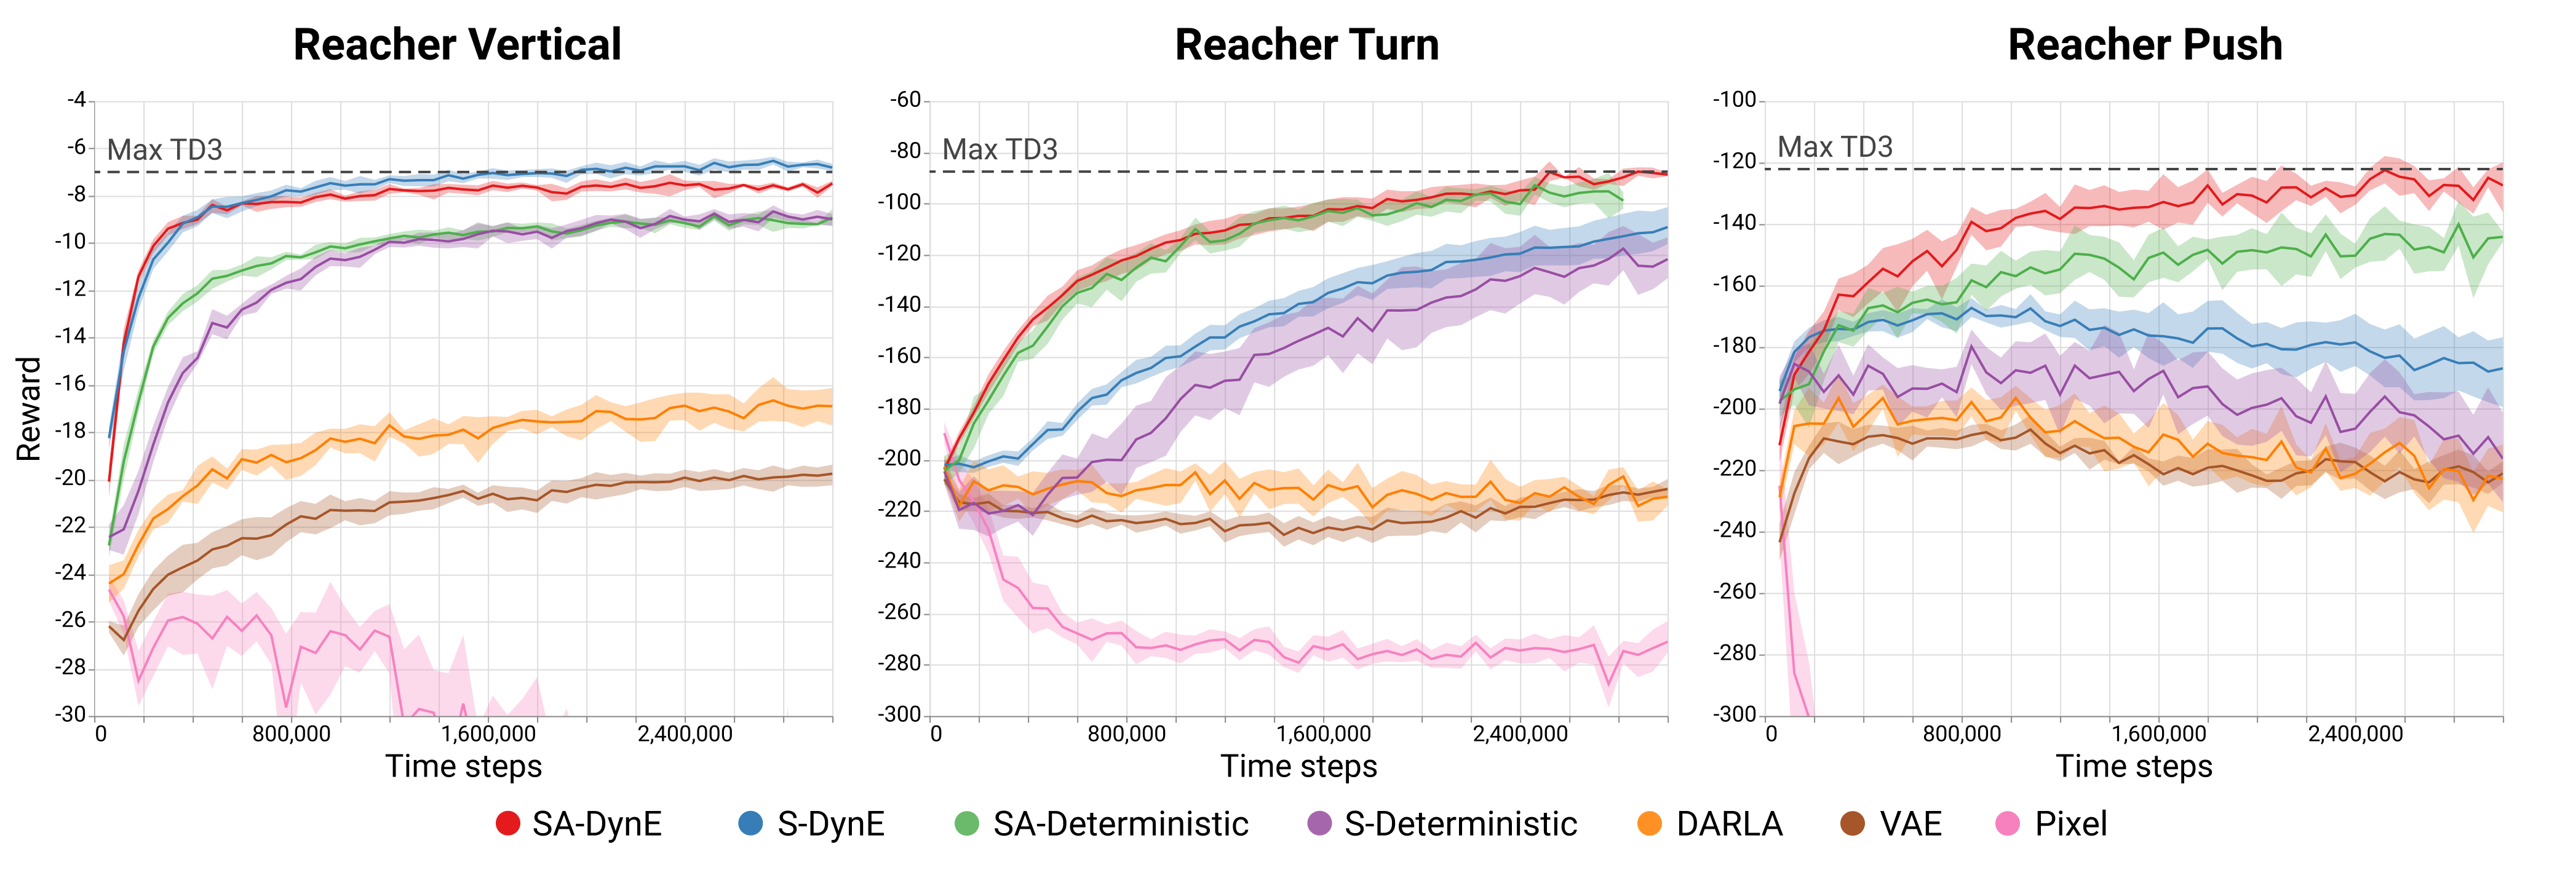
\includegraphics[width=0.95\textwidth]{figures/dyne/pixels_results_sdet.png}
\caption{Performance of TD3 trained with various representations.
Learned representations for state which incorporate the dynamics make a dramatic difference.
SA-DynE converges stably and rapidly and achieves performance from pixels that nearly equals TD3's performance from states.
Dark lines are mean reward over 8 seeds and shaded areas are bootstrapped 95\% confidence intervals.}
\label{fig:pixel_results}
\end{figure}

\paragraph{Results}
Figure~\ref{fig:pixel_results} shows the results of these experiments.
We find that the single-image methods are unable to solve any of the three tasks from pixels; TD3 from pixels diverges in all cases, while VAE and DARLA learn gradually at best.
If simply reducing the dimension of the states were sufficient to enable effective policy training, we would expect good performance from these methods.
S-DynE and S-Deterministic, which incorporate the dynamics into their representation learning objectives, perform far better.
The minimality imposed by the DynE objective allows S-DynE and SA-Dyne to outperform their deterministic ablations.
% Instead we find that S-DynE-TD3 trains with many fewer samples and reaches higher performance than VAE-TD3, demonstrating that the particular structure learned by DynE plays a crucial role in learning.
% S-DynE-TD3 is able to achieve decent performance on the two simpler environments, establishing a lower bound on the fidelity of the DynE state representation.
SA-DynE learns rapidly and reliably, finding behaviors which qualitatively solve all three tasks.
The improvement of SA-DynE over S-DynE shows that the state and action representations are complementary.

% Furthermore, training a policy from pixels using SA-DynE-TD3 has dramatically better sample complexity than training PPO from low-dimensional states across all three environments and equals SAC from low-d states on \texttt{ReacherTurn}.
% For a comparison of these methods across different observation spaces see Appendix \labelcref{sec:extended_results}.
% These results show that the DynE action and state representations are effective at scaling model-free RL to environments with high-dimensional states and difficult exploration.




\section{Discussion}

In this work we proposed a method, Dynamics-aware Embedding (DynE), that jointly learns embedded representations of states and actions for reinforcement learning.
% We described how DynE embeddings exhibits the properties of fidelity, structure, and reach and how they affect policy learning.
Our experiments reveal that DynE action embeddings lead to more efficient exploration, resulting in more sample efficient learning on complex tasks, while DynE state embeddings allow unmodified model-free RL algorithms to scale to pixel observations.
When combined, the DynE state and action embeddings result in stable, sample-efficient learning of high-quality policies from pixels.

\side{add appendices}

\printendnotes

\part{Improving Performance with \\Batched Data} \label{sec:offline}
Introduction to offline RL.

\chapter{Offline Contextual Bandits with Overparameterized Models} \label{sec:offline-bandits}
\newcommand{\one}{\mathbbm{1}}

\section{Introduction}

% In the offline contextual bandit problem, we are given a dataset of context, action, reward tuples collected by some behavior policy, and the goal is to learn a new policy which maximizes the expected reward.
% The problem can represent many decision making applications. For example, problems in recommender systems \citep{li2010contextual, bottou2013counterfactual}, healthcare \citep{Prasad2017ARL, Raghu2017DeepRL}, and robotics \citep{pinto2016supersizing} can all be cast as offline policy learning problems.
% In these domains it is often critical to be able to learn the policy offline without deploying untrained algorithms in the real world.

%An important class of machine learning problems is given by offline contextual bandits.
The offline contextual bandit problem can be used to model decision making from logged data in domains as diverse as recommender systems \citep{li2010contextual, bottou2013counterfactual}, healthcare \citep{Prasad2017ARL, Raghu2017DeepRL}, and robotics \citep{pinto2016supersizing}.
Prior work on the problem has primarily focused on underparameterized models with finite and small VC dimensions. This work has come from the bandit literature \citep{strehl2010learning, swaminathan2015counterfactual, swaminathan2015self}, the reinforcement learning literature \citep{munos2008finite, chen2019information}, and the causal inference literature \citep{bottou2013counterfactual, athey2017efficient, kallus2018balanced, zhou2018offline}.



%The offline contextual bandit is superficially similar to supervised learning, with the only difference being that feedback is only given for the selected action rather than the full feedback observed in a supervised problem.
In contrast, the best performance in modern supervised learning is often achieved by massively overparameterized models that are capable of fitting random labels \citep{zhang2016understanding}. Use of such large models renders vacuous the bounds that require a small model class. But, the massive capacity of popular neural network models is now often viewed as a feature rather than a bug. Large models reduce approximation error and allow for easier optimization \citep{du2018gradient} while still being able to generalize in regression and classification problems \citep{belkin2018overfitting, belkin2019does}.
In this paper, we investigate whether the strong performance of overparameterized models in supervised learning translates to the offline contextual bandit setting.
The main prior work that considers this setup is \citep{joachims2018deep}, which we discuss in detail in Section~\ref{sec:related}.



To formalize the differences between the supervised learning and contextual bandit settings, we introduce a novel regret decomposition.
This decomposition shares the approximation and estimation terms from classic work in supervised learning \citep{vapnik1982, bottou2008tradeoffs}, but adds a term for ``bandit'' error which captures the excess risk due to only receiving partial feedback.

% To frame our discussion, we introduce a novel regret decomposition into approximation, estimation, and ``bandit'' errors.
% %The bandit error measures the expected difference between the value of a policy learned from a full feedback dataset and one learned from a bandit feedback dataset.
% This extends prior work from supervised learning that decomposes excess risk into estimation and approximation error \citep{vapnik1982, bottou2008tradeoffs} by adding the bandit error.
% The bandit error captures the error that is due to only observing the action selected by the behavior policy at each point in the dataset.

We use this framework to address the question: can we use overparameterized models for offline contextual bandits? Or is the bandit error a fundamental problem when we use large models?
We find mixed results.
Value-based algorithms benefit from the same generalization behavior as overparameterized supervised learning, but policy-based algorithms do not.
We show that this difference is explained by a property of their objectives called \emph{action-stability}.
An objective is action-stable if there exists a single prediction which is simultaneously optimal for any observed action (where a ``prediction'' is a vector of state-action values for a value-based objective or an action distribution for a policy-based objective).
%\rr{i'm tempted to say something stronger that overparamterization is important for action-stable since if the model is not flexible enough, the random sampled actions from the behavior can bend the model inappropriately}
Action-stable objectives perform well when combined with overparameterized models since the random actions taken by the behavior policy do not change the optimal prediction.
However, interpolating an unstable objective results in learning a different function for every sample of actions, even though the true optimal policy remains unchanged.

% We show that this discrepancy is due to the \emph{action-stability} of their objectives.

% We focus on understanding the offline policy learning problem better by focusing on the issue of overfitting. Understanding overfitting is especially important in a modern context where we often use overparameterized models that are capable of interpolating the training data. We show that there are important distinctions in (1) how overfitting impacts policy learning versus supervised learning and (2) how overfitting impacts policy-based versus value-based algorithms.


% We also introduce the concept of an ``action-stable'' objective function. An objective is action-stable at a datapoint if there exists a model output which optimizes the objective regardless of which action is sampled from the behavior.
% Intuitively, an algorithm that is not action-stable will be sensitive to noise in the behavior policy and thus have large bandit error.
%This decomposition is conceptually useful because it allows us to disentangle the the estimation error, which captures overfitting due to noise in the rewards, from the bandit error due to the actions.

%This gives us a notion of bandit overfitting which extends the idea of  ``propensity overfitting'' from \cite{swaminathan2015self, joachims2018deep}.
%This introduction of bandit error emphasizes the difference between overfitting in policy learning as compared to supervised learning.

%Armed with this framework, we compare policy-based and value-based algorithms in the overparameterized setting.
%for solving the offline policy learning problem.
%While the methods perform similarly in the classical setting of small model classes,

On the theory side, we prove that overparameterized value-based algorithms are action stable and have small bandit error via reduction to overparameterized regression.
Meanwhile we prove that policy-based algorithms are not action-stable which allows us to prove lower bounds on the ``in-sample'' regret and lower bounds on the regret for simple nonparametric models.
%, and a formal connection between noisy classification and policy-based learning.

Empirically, we demonstrate the gap in both action stability and bandit error between policy-based and value-based algorithms when using large neural network models on synthetic and image-based datasets.


%This paper presents the first analysis of the offline contextual bandit problem when using overparameterized models.
In summary, our main contributions are:
\begin{itemize}
    % \item We conduct the first analysis of the offline contextual bandit problem when using overparameterized models.
    \item We introduce the concept of bandit error, which separates contextual bandits from supervised learning.
    \item We introduce action-stability and show that a lack of action-stability causes bandit error.
    % \item We decompose regret  bandit error and action-stable algorithms.
    \item We show a gap between policy-based and value-based algorithms based on action-stability and bandit error both in theory and experiments. %While value-based algorithms are action-stable, policy-based algorithms are not. This leads to high bandit error and high regret for policy-based algorithms when we use overparameterized models.
\end{itemize}


%We compare the statistical rates of the bounds in the case of small model classes from existing work. Then we move on to the case of overparameterized models. In this setting, we show that value-based methods can recover guarantees of overparameterized regression via a reduction. Policy-based methods, however, do not have similar guarantees. We highlight this by showing that a nearest neighbors policy cannot recover the optimal policy even in the limit of infinite data with noiseless rewards.

% Finally, we experimentally confirm that the intuitions from the theory hold beyond the strict settings of the theory itself. Specifically, we look at neural network models on toy problems, problems with real images as contexts, and a simulated economic problem. We find that indeed policy-based algorithms suffer from bandit overfitting more than their value-based counterparts in these overparameterized settings.







\section{Setup}\label{sec:setup}
\subsection{Offline contextual bandit problem}

First we will define the contextual bandit problem \citep{langford2008epoch}. Let the context space $ \mathcal{X} $ be infinite and the action space $ \mathcal{A}$ be finite with $ |\mathcal{A}| = K < \infty$.
At each round, a context $ x \in \mathcal{X}$ and a full feedback reward vector $ r \in [r_{\mathrm{min}},r_{\mathrm{max}}]^K$ are drawn from a joint distribution $ \mathcal{D}$.
Note that $ r $ can depend on $ x $ since they are jointly distributed.
A policy $\pi: \mathcal{X} \to \mathcal{P}(\mathcal{A})$ maps contexts to distributions over actions. An action $ a $ is sampled according to $ \pi(a|x)$ and the reward is $ r(a)$, the component of the vector $ r $ corresponding to $ a$.
We use ``bandit feedback'' to refer to only observing $ r(a)$.
This contrasts with the ``full feedback'' problem
%of cost-sensitive classification
where at each round the full vector of rewards $ r$ is revealed, independent of the action.

In the offline setting there is a finite dataset of $ N $ rounds with a fixed behavior policy $ \beta$.  Then we denote the dataset as $ S = \{x_i, r_i, a_i, p_i\}_{i=1}^N$ where $ p_i $ is the observed propensity $ p_i = \beta(a_i|x_i)$. The tuples in the datasets lie in $ \mathcal{X} \times [r_{min},r_{max}]^K \times \mathcal{A} \times [0,1]$ and are drawn i.i.d from the joint distribution induced by $ \mathcal{D}$ and $ \beta$.
From $ S $ we define the datasets $ S_B$ for bandit feedback and $ S_F$ for full feedback:
\begin{align*}
    S_B = \{(x_i, r_i(a_i), a_i, p_i)\}_{i=1}^N, \quad S_F = \{(x_i, r_i)\}_{i=1}^N.
\end{align*}
Note that we are assuming access to the behavior probabilities $ p_i = \beta(a_i|x_i)$, so the issues that we raise do not have to do with estimating propensities.
We will further make the following assumption about the behavior.
\begin{assumption}[Strict positivity]\label{ass:positivity}
We have strict positivity of $ \tau $ if $ \beta(a|x) \geq \tau > 0$ for all $ a, x$. Thus, in any dataset we will have $ p_i = \beta(a_i|x_i) \geq \tau > 0$.
\end{assumption}
There is important work that focuses learning without strict positivity by making algorithmic modifications like clipping \citep{bottou2013counterfactual, strehl2010learning, swaminathan2015counterfactual} and behavior constraints \citep{fujimoto2018off, laroche2019safe}. However, these issues are orthogonal to the main contribution of our paper, so we focus on the setting with strict positivity.

% Note that we are assuming access to the behavior probabilities $ \beta(a_i|x_i) $. This assumption likely holds in settings where the behavior policy is another algorithm, but not when it is a human.
% Importantly, our negative results hold even in this best-case setting.
% When the behavior probabilities are unavailable, results can often be extended by learning a model of the propensities \citep{strehl2010learning}.


The goal of an offline contextual bandit algorithm is to take in a dataset and produce a policy $ \pi$ so as to maximize the value $ V(\pi)$ defined as
\begin{align*}
    V(\pi) := \E_{x, r \sim \mathcal{D}}\E_{a \sim \pi(\cdot|x)} [r(a)].
\end{align*}
We will use $ \pi^*$ to denote the deterministic policy that maximizes $ V$.
Finally, define the $ Q $ function at a particular context, action pair as
\begin{align*}
    Q(x,a) := \E_{r|x}[r(a)].
\end{align*}


\subsection{Model classes}

The novelty of our setting comes from the use of overparameterized model classes that are capable of interpolating the training objective.
To define this more formally, all of the algorithms we consider take a model class of either policies $ \Pi$ or $ Q$ functions $ \mathcal{Q}$ and optimize some objective over the data with respect to the model class.
Following the empirical work of \cite{zhang2016understanding} and theoretical work of \cite{belkin2018overfitting} we will call a model class ``overparameterized'' or ``interpolating'' if the model class contains a model that exactly optimizes the training objective. Formally, if we have data $ \{x_i\}_{i=1}^N$ and a pointwise loss function $ \ell(x, y)$, then a model class $ \Pi$ can interpolate the data if
\begin{align*}
    \inf_{\pi\in \Pi} \sum_{i=1}^N \ell(x_i, \pi(x_i)) = \sum_{i=1}^N \inf_{y} \ell(x_i, y).
\end{align*}
This contrasts with traditional statistical learning settings where we assume that the model class is finite or has low complexity as measured by something like VC dimension \cite{strehl2010learning, swaminathan2015counterfactual}.


\subsection{Algorithms}\label{sec:basic-algs}

Now that we have defined the problem setting, we can define the algorithms that we will analyze. This is not meant to be a comprehensive account of all algorithms, but a broad picture of the ``vanilla'' versions of the main families of algorithms. Since we are focusing on statistical issues we do not consider how the objectives are optimized.

\paragraph{Supervised learning with full feedback.} In a full feedback problem, empirical value maximization (the analog to standard empirical risk minimization) is defined by maximizing the empirical value $ \hat V_F$:
\begin{align}
    \hat V_F(\pi; S_F) &:= \frac{1}{N}\sum_{i=1}^N \langle r_i, \pi(\cdot|x_i)\rangle\\  \pi_F &:= \arg\max_{\pi\in \Pi} \hat V_F(\pi;S_F).
\end{align}


\paragraph{Policy-based learning.}
Importance weighted or ``inverse propensity weighted'' policy optimization directly optimizes the policy to maximize an estimate of its value. Since we only observe the rewards of the behavior policy, we use importance weighting to get an unbiased value estimate to maximize. Explicitly:
\begin{align}
    \hat V_B(\pi ; S_B) &:= \frac{1}{N}\sum_{i=1}^N r_i(a_i) \frac{\pi(a_i|x_i)}{p_i} \\ \pi_B &:= \arg \max_{\pi \in \Pi} \hat V_B(\pi;S_B). \label{eq:pi}
\end{align}
Note that this is the ``vanilla'' version of the policy-based algorithm and modifications like regularizers, baselines/control variates, clipped importance weights, and self-normalized importance weights have been proposed \citep{bottou2013counterfactual, joachims2018deep, strehl2010learning, swaminathan2015counterfactual, swaminathan2015self}.
For our purposes considering this vanilla version is sufficient since as we show in Section \ref{sec:stable}, any objective that takes the form $ \pi(a_i|x_i) f(x_i, a_i, r_i, p_i)$ at each datapoint will have the same sort of problem with action-stability.



It is important to note that with underparameterized model classes, this algorithm is guaranteed to return nearly the best policy in the class. Explicilty, \citet{strehl2010learning} prove that for a finite policy class $ \Pi$, with high probability the regret of the learned policy $ \pi_B$ is bounded as $ O(\frac{1}{\tau} \sqrt{\frac{\log |\Pi|}{N}})$. This is elaborated in Appendix \ref{app:small}. However, these guarantees no longer hold in our overparameterized setting.

% The most relevant modification for our analysis is the introduction of constant baselines \citep{williams1992simple, joachims2018deep}. Adding a baseline $ b $ modifies the algorithm as follows:
% \begin{align} \label{eq:pi_baseline}
%     \hat V_{B,b}(\pi;S_B) &:= \frac{1}{N}\sum_{i=1}^N (r_i(a_i) - b) \frac{\pi(a_i|x_i)}{p_i}\\ \pi_{B,b} &:= \arg \max_{\pi \in \Pi} \hat V_{B,b}(\pi;S_B).
% \end{align}
% This modification is discussed in Sections \ref{sec:baselines} and \ref{sec:exp_base}.

\paragraph{Value-based learning.}
Another simple algorithm is to first learn the $ Q $ function and then use a greedy policy with respect to this estimated $ Q$ function. Explicitly:
\begin{align}\label{eqn:hatQ}
    \hat Q_{S_B} &:= \arg\min_{f \in \mathcal{Q}} \sum_{i=1}^N (f(x_i, a_i) - r_i(a_i))^2 \\ \pi_{\hat Q_{S_B}}(a|x) &:= \one \left[a = \arg\max_{a'} \hat Q_{S_B}(x, a')\right].
\end{align}
This algorithm is sometimes called the ``direct method'' \citep{dudik2011doubly}.
The RL literature also often defines a class of model-based algorithms, but in the contextual bandit problem there are no state transitions so model-based algorithms are equivalent to value-based algorithms.


This algorithm also has a guarantee with small model classes. Explicilty, \citet{chen2019information} prove that for a finite \emph{and well specified} model class $ \mathcal{Q}$, with high probability the regret of the learned policy $ \pi_{\hat Q_{S_B}}$ is bounded as $ O(\frac{1}{\sqrt{\tau}} \sqrt{\frac{\log |\mathcal{Q}|}{N}})$. This is elaborated in Appendix \ref{app:small}. Again, these guarantees no longer hold in our overparameterized setting.


\paragraph{Doubly robust policy optimization.}

The class of doubly robust algorithms \citep{dudik2011doubly} does not fall cleanly into the value-based or policy-based bins since it requires first learning a value function and using that to optimize a policy. However, with overparamterized models, doubly robust learning becomes exactly equivalent to our vanilla value-based algorithm unless we use crossfitting since the estimated Q values will coincide with the rewards. We prove this formally in Appendix \ref{app:dr} where we also show some issues that the doubly robust policy objective can have with overparameterized models and highly stochastic rewards. For our purposes, we will only consider the policy-based and value-based approaches since the doubly robust approach collapses to the value-based approach with overparameterized models.






\section{Bandit error}\label{sec:decomp}


In supervised learning, the standard decomposition of the excess risk separates the approximation and estimation error  \citep{bottou2008tradeoffs}. The approximation error is due to the limited function class and the estimation error is due to minimizing the empirical risk rather than the true risk. Since the full feedback policy learning problem is equivalent to supervised learning, the same decomposition applies. Formally, consider a full feedback algorithm $ \mathcal{A}_F$ which takes the dataset $ S_F $ and produces a policy $ \pi_F$. Then
\begin{align*}
    &\underbrace{\E_{S}[V(\pi^*) - V(\pi_F)]}_{\textrm{regret}} = \underbrace{V(\pi^*) - \sup_{\pi\in \Pi}V(\pi)}_{\textrm{approximation\ error}} + \underbrace{\E_{S}[ \sup_{\pi\in \Pi}V(\pi) - V(\pi_F)]}_{\textrm{estimation\ error}}.
\end{align*}
We can instead consider a bandit feedback algorithm $ \mathcal{A}_B$ which takes the dataset $ S_B $ and produces a policy $ \pi_B$.
To extend the above decomposition to the bandit problem we add a new term, the bandit error, that results from having access to $ S_B$ rather than $ S_F$. Now we have:
\begin{align*}
    &\underbrace{\E_{S}[V(\pi^*) - V(\pi_B)]}_{\textrm{regret}} = \underbrace{V(\pi^*) - \sup_{\pi\in \Pi}V(\pi)}_{\textrm{approximation\ error}} + \underbrace{\E_{S}[ \sup_{\pi\in \Pi}V(\pi) - V(\pi_F)]}_{\textrm{estimation\ error}} + \underbrace{\E_{S}[V(\pi_F) - V(\pi_B)]}_{\textrm{bandit\ error}}.
\end{align*}

\paragraph{Disentangling sources of error.}
The approximation error is the same quantity that we encounter in the supervised learning problem, measuring how well our function class can do.
The estimation error measures the error due to overfitting on finite contexts and noisy rewards.
The bandit error accounts for the error due to only observing the actions chosen by the behavior policy.
This is not quite analogous to overfitting to noise in the rewards since stochasticity in the actions is actually required to have the coverage of context-action pairs needed to learn a policy.
While the standard approximation-estimation decomposition could be directly extended to the bandit problem, our approximation-estimation-bandit decomposition is more conceptually useful since it disentangles these two types of error.




\paragraph{Can bandit error be negative?}
Usually, we think about an error decomposition as a sum of positive terms.
This is not necessarily the case with our decomposition, but we view this as a feature rather than a bug.
Intuitively, the bandit error term captures the contribution of the actions selected by the behavior policy.
If the behavior policy is nearly optimal and the rewards are highly stochastic, there may be more signal in the actions selected by the behavior policy than the observed rewards.
Thus overfitting the actions chosen by behavior policy can sometimes be beneficial, causing the bandit error to be negative.
The two terms disentangle the approximation error (due to reward noise) from bandit error (due to behavior actions).






\section{Action-stable objective functions}\label{sec:stable}

% As alluded to above, our main result is that bandit error is a more pronounced problem for policy-based than value-based algorithms when we have over-parameterized models.
% At first it may seem that policy-based algorithms are a more intuitive approach than value-based algorithms since a policy-based approach directly optimizes an estimate of our ultimate goal to find a policy with high value.
% However, as we will explain in this section, policy-based approaches use objectives that are not ``action-stable''.
% This means that at a single context the objective is optimized by a different policy at each depending on which action is sampled.

Consider a simple thought experiment.
We collect a contextual bandit dataset $S_B$ from a two-action environment using a uniformly random behavior policy.
Then we construct a second dataset $\widetilde S_B$ by evaluating the outcome of taking the opposite action at each observed context.
Since nothing about the environment has changed, we know that the optimal policy remains the same.
Therefore we desire the following property from a bandit objective: there exists a single model which is optimal (with respect to that objective) on both $S_B$ and $\widetilde S_B$.
We say that such an objective is \emph{action-stable} because it has an optimal policy which is stable to re-sampling of the actions in the dataset.

% Intuitively, the optimal action in a given context does not depend on the action which the behavior policy chose.
% An action-stable objective is one which captures this intuition: there is a prediction which minimizes the loss no matter

More formally, we define action stability pointwise at a datapoint $ z = (x,r,p)$ where $ r\in [r_{\min}, r_{\max}]^K$ and $ p \in \Delta^K$ is the behavior probability vector in the $K$-dimensional simplex (recall that $ K $ is the number of the actions). Let $ z(a)$ denote the datapoint when action $ a $ is sampled so that $ z(a) = (x, r(a), p(a), a)$. The objectives for both policy and value-based algorithms decompose into sums over the data of some loss $ \ell(z(a), \pi(a|x))$ or $ \ell(z(a), Q(x,a))$.

Note that the output space of a policy is the simplex so that $ \pi(\cdot|x) \in \Delta^K$, while the output of a Q function\endnote{When using neural networks Q is usually implemented as a function of $ x $ with $ K $ outputs \cite{mnih2015human}.} is $ Q(x, \cdot) \in \R^K$.
To allow for this difference in our definition, we will define a generic $ K$-dimensional output space $ \mathcal{Y}^K$ and its corresponding restriction to one dimension as $ \mathcal{Y}$.
So for a policy-based algorithm $ \mathcal{Y}^K = \Delta^K$ and $ \mathcal{Y} = [0,1]$, while for a value-based algorithm $ \mathcal{Y}^K = \R^K$ and $ \mathcal{Y} = \R$. Now we can define action-stability.

\begin{definition}[Action-stable objective]
An objective function $ \ell$ is action-stable at a datapoint $ z$ if there exists $ y^* \in \mathcal{Y}^K$ such that for all $ a \in \mathcal{A}$:
\begin{align*}
    \ell(z(a), y^*(a)) = \min_{y \in \mathcal{Y}} \ell(z(a), y).
\end{align*}
\end{definition}

% An objective which is action stable
If an objective is not action-stable, a function which minimizes that objective exactly at every datapoint $(x, r(a), p(a), a)$ does \emph{not} minimize it for a different choice of $a$.
As a direct consequence, interpolating an unstable objective results in learning a different function for every sample of actions, even though the true optimal policy remains unchanged.

We find that policy-based objectives are not action-stable, while value-based objectives are.
In the next section we will use the instability of policy-based objectives to show that policy-based algorithms exhibit large bandit error when used with overparameterized models.
Our stability results are stated in the following two Lemmas, whose proofs can be found in Appendix \ref{app:stable}.

% % Our main result is that bandit error is a more pronounced problem for policy-based than value-based algorithms when we have over-parameterized models.
% At first it may seem that policy-based algorithms are a more intuitive approach since they directly optimize an estimate of our ultimate objective: the value of the learned policy.
% However, policy-based approaches use objectives that are not action-stable (i.e. stable to re-sampling of the actions in the dataset).
% %This means that at a single context the objective is optimized by a different policy depending on which action was observed.
% This instability prevents generalization when using an overparameterized model that can optimize the policy nearly independently at each context.
% Policy-based algorithms end up treating the stochasticity in the behavior policy as noise in the objective which causes large bandit error; value-based algorithms, meanwhile, leverage that stochasticity as coverage that helps to evaluate counterfactuals.



% A decomposable algorithm is a function $ f: z(a) \to \mathcal{P}(\Delta^K)$

% \begin{definition}
% A decomposable algorithm $ f $ is action-stable at a datapoint $ z $ if there exists a probability vector $ y^* \in \Delta^K$ such that for all $ a \in \mathcal{A}$,
% \begin{align*}
%     y^* \in f(z(a))
% \end{align*}
% \end{definition}




\begin{restatable}[Value-based stability]{lemma}{vbstable}\label{lem:vb-stable}
Value-based objectives are action stable since we can let $ y^* = r$ and this minimizes the square loss at every action.
\end{restatable}

\begin{restatable}[Policy-based instability]{lemma}{pbstable}\label{lem:pb-stable}
All policy-based objectives which take the form \newline$\ell(z(a), \pi(a|x)) = f(z(a)) \pi(a|x)$ are not action-stable at $ z$ unless $ f(z(a)) > 0$ for exactly one action $ a$.
\end{restatable}

These Lemmas tell us that the stochasticity of the behavior policy can cause instability for policy-based objectives.
This is worrisome since one would hope that more stochastic behavior policies give us more information about all the actions and should thus yield better policies. Indeed, this is the case for value-based algorithms as we will see in the next section. But for policy-based algorithms, stochastic behavior can itself be a cause of overfitting due to the instability of the objective function.

\paragraph{Stabilizing policy-based algorithms.} To avoid this problem in a policy-based algorithm, the sign of the function $f(z(a))$ must indicate the optimal action. This essentially requires having access to a \emph{baseline} function $ b(s) $ that separates the optimal action from all the others so that $ r(a) > b(s)$ if and only if $ a $ is the optimal action. And then $  f(z(a)) = \frac{r(a) - b(s)}{\beta(a|s)}$ yields an action-stable algorithm. This is in general as difficult as learning the full value function $ Q$. One notable special case is when the bandit problem is induced by an underlying classification problem, so that only one action has reward 1 and all others have 0. In this case, any constant baseline between 0 and 1 will lead to action stability. This case has often been considered in the literature, e.g. by \citet{joachims2018deep} as we discuss in Section \ref{sec:related}.


Now that we have built up an understanding of the problem we can prove some formal results that show how value-based algorithms more effectively leverage overparameterized models by being action-stable.


\section{Regret bounds}

Recall that as explained in Section~\ref{sec:setup}, both policy-based and value-based algorithms have regret guarantees when we use small model classes \cite{strehl2010learning, chen2019information}. But, when we move to the overparameterized setting, this is no longer the case. In this section we prove regret upper bounds for value-based learning by using recent results in overparameterized regression. Then we prove lower bounds on the regret of policy-based algorithms due to their action-instability.

\subsection{Value-based learning}

In this section we show that value-based algorithms can provably compete with the optimal policy.
The key insight is to reduce the problem to regression and then leverage the guarantees on overparameterized regression from the supervised learning literature.
This is formalized by the following theorem.

% While policy optimization can be sensitive to bandit overfitting, we will show that value-based learning is not when we make some structural assumptions on the true $Q$ function.
% The following theorem reduces bounding the regret of value-based learning to bounding the generalization of the learned $Q$ function.
% This makes work about generalization of interpolating regression directly applicable.
%These include one nearest neighbor under no reward noise, overparameterized linear regression, interpolating kernel methods, and overparameterized neural networks, which can all recover good finite sample statistical convergence rates.

\begin{restatable}[Reduction to regression]{theorem}{reduction}\label{thm:reduction}
By Assumption~\ref{ass:positivity} we have $ \beta(a|x) \geq \tau$ for all $ x,a$. Then with $ \hat Q_{S_B}$ as defined in (\ref{eqn:hatQ}) we have
\begin{align*}
    V(\pi^*) - V(\pi_{\hat Q_{S_B}}) \leq \frac{2}{\sqrt{\tau}} \sqrt{\mathop{\mathbb{E}}_{x, a \sim \beta}[(Q(x,a) - \hat Q_{S_B}(x,a))^2]}.
\end{align*}
\end{restatable}

A proof can be found in Appendix \ref{app:value}. Similar results are presented as intermediate results in \citet{chen2019information, munos2008finite}.
The implication of this result that we want to emphasize is that any generalization guarantees for overparameterized regression immediately become guarantees for value-based learning in offline contextual bandits. Essentially, Theorem \ref{thm:reduction} gives us a regret bound in any problem where overparameterized regression works.
The following results from the overparameterized regression literature demonstrate a few of these guarantees, which all require some sort of regularity assumption on the true $Q$ function to bound the regression error:

%Note that we are less worried about model misspecification in the overparameterized setting, but these sorts of structural assumptions on $ Q $ are essentially ensuring the model is well specified.

%To explicitly connect to guarantees on regression, we need to decide how $ Q(x,a)$ depends on $ a $ which is a categorical variable. Generally, it is natural to learn $ K $ separate regressors, one for each action.

%\paragraph{Interpolating regression guarantees.}

\begin{itemize}
    \item The results of \cite{bartlett2020benign} give finite sample rates for overparameterized linear regression by the minimum norm interpolator depending on the covariance matrix of the data and assuming that the true function is realizable.
    \item The results of \cite{belkin2019does} imply that under smoothness assumptions on $ Q$, a particular singular kernel will interpolate the data and have optimal non-parametric rates. After applying our reduction, the rates are no longer optimal for the policy learning problem due to the square root.
    \item The results of \cite{bach2017breaking} show how choosing the minimum norm infinite width neural network in a particular function space can yield adaptive finite sample guarantees for many types of underlying structure in the $ Q $ function.
    \item The results of \cite{cover1968estimation} imply the consistency of a one nearest neighbor regressor when the rewards are noiseless and $ Q $ is piecewise continuous. This will contrast nicely with Theorem \ref{thm:nn} below.
\end{itemize}
Each of these guarantees implies a corresponding corollary to Theorem \ref{thm:reduction} resulting in a regret bound for that particular combination of model and assumptions on $ Q$.



\subsection{Policy-based learning}

Now we will show how the policy-based learning algorithms can provably fail because they lack action-stability. We will do this in a few ways. First, we will show that on the contexts in the dataset an action-unstable algorithm must suffer regret. This means that we cannot even learn the optimal policy at the contexts seen during training. Then to deal with generalization beyond the dataset we will prove a regret lower bound for a specific overparameterized model, namely one nearest neighbor. Finally, we discuss a conjecture that such lower bounds can be extended to richer model classes like neural networks.
%Finally, we will show that in general we can think of action-instability causing policy-based algorithms to behave like classification algorithms trained a noisy dataset where the noise is added by the behavior policy.

Since we are proving lower bounds, making any more simplifying assumptions only makes the bound stronger. As such, all of our problem instances that create the lower bounds have only two actions ($ K = 2$).

\paragraph{Regret on the observed contexts.} Before considering how a policy generalizes off of the data, it is useful to consider what happens at the contexts in the dataset. This is especially true for overparameterized models which can exactly optimize the objective on the dataset. To do this, we will define the value of a policy $ \pi$ on the contexts in a dataset $ S $ (which we will call the ``in-sample'' value) by
\begin{align}
    V(\pi; S) := \frac{1}{N}\sum_{i=1}^N \E_{r|x_i}\E_{a\sim \pi(\cdot|x_i)}[r(a)].
\end{align}
Then the following Theorem shows that the policy $\pi_B$ learned by the simple policy-based algorithm in Equation (\ref{eq:pi}) must suffer substantial regret on $S$.

\begin{restatable}[In-sample regret lower bound]{theorem}{vsthm}\label{thm:vs}
Let $ K=2$ and the policy class be overparameterized.
Define $ \Delta_r(x) = \left|\E_{r|x} [r(1) - r(2)]\right|$ as the absolute expected gap in rewards at $ x$.
Define $p_u(x)$ to be the probability that the policy-based objective is action-unstable at $ x$. Recall that $ \beta(a|x) \geq \tau$ by Assumption \ref{ass:positivity}.
%$ U_{x,r}$ to be the event that the policy-based objective is action-unstable at $ x, r$.
%and $ p_s = \E_{x,r}[\one[E_{x,r}]]$ to be the probability that objective is action-stable.
%Assume that $ E_{x,r} \perp a | x$ so that stability is independent from the the behavior.
Then
\begin{align*}
    \E_S[V(\pi^*;S) - &V(\pi_B; S)] \geq  \tau \E_{x}\big[ p_u(x) \Delta_r(x)\big].  %\frac{ \Delta_r}{2} (1 - p_{stable}).
\end{align*}
\end{restatable}

The full proof is in Appendix \ref{app:pb}.
This Theorem tells us that as often as the objective is action-unstable, we can suffer substantial regret even \emph{on the contexts in the dataset}. We now offer some brief intuition of the proof. When we have two actions and an algorithm is not action-stable at $ x $, then action chosen by the learned policy $ \pi_B$ at $ x_i$ is directly dependent on the observed action $ a_i$. Since the behavior $ \beta$ will choose each action with probability at least $ \tau$ by Assumption \ref{ass:positivity}, the learned policy $ \pi_B$ must choose the suboptimal action with probability at least $ \tau$ at $ x_i$. This causes unavoidable regret for unstable algorithms, as formally stated in Theorem \ref{thm:vs}.

Note that Theorem \ref{thm:vs} essentially says that action-unstable algorithms convert noise in the behavior into regret. This is the essential problem with unstable algorithms. Rather than using stochasticity in the behavior policy to get estimates of counterfactual actions, an action-unstable algorithm is sensitive to this stochasticity like it is label noise in supervised learning.

In Appendix \ref{app:noisy} we present a result that makes this connection between behavior policy noise and action-instability more direct. Specifically we show a reduction that takes any classification problem and turns it into a bandit problem such that optimizing the policy-based objective is equivalent to solving a noisy variant of the classification problem. On the contrary, optimizing the full-feedback objective is equivalent to the noiseless classification problem.

The limitation of this result is that it only applies in-sample and does not rule out that the model class could leverage its inductive bias to perform well away from the training data.
Next we convert this in-sample regret lower bound into a standard regret lower bound for a particular simple interpolating model class, the nearest neighbor policy.



\paragraph{Regret with generalization: nearest neighbor models.}

The above result shows what happens at the contexts \emph{in the dataset} $ S$. It seems that only pathological combinations of model class and problem instance could perform poorly on $ S$ but recover strong performance off of the data. However, it cannot be ruled out a priori if the model class has strong inductive biases to generalize well. In this section we will show that at least for a very simple overparameterized model class, the generalization of the model does not improve performance.

The following theorem shows that the simplest interpolating model class, a one nearest neighbor rule, fails to recover the optimal policy even in the limit of infinite data.


% Our first regret bound considers perhaps the simplest interpolator, a nearest neighbor policy. We use this to illustrate that even with noiseless rewards and infinite data, bandit overfitting can prevent an interpolating policy class from finding the optimal policy. Moreover, we demonstrate the dependence on the behavior policy by incorporating the probability that the behavior policy chooses an optimal action. As hinted at in the example above, when the rewards are positive the policy is encouraged to clone the behavior and when the rewards are negative the policy will anti-clone the behavior. This tendency allows us to construct problems much like the motivating example where nearest neighbor policies will fail to recover the optimal policy since they fit the behavior actions rather than the rewards.


% The next question is what happens when we take this bad signal and try to generalize away from the observed context.
% We will start by considering a nearest neighbor rule in the following theorem, whose proof can be found in Appendix \ref{app:po}.


% \begin{definition}[Local generalization]
% Let $ i(x) $ be the index of the nearest neighbor of $ x $ in the dataset $ S $. Let $\hat a_i$ be the action that optimizes $ r_i(a_i) \frac{\one[a_i = \hat a_i]}{p_i}$. A policy $ \pi$ generalizes locally if there exists a constant $ c_g > 0$ such that $ P_{x, a \sim \pi|x}(a = \hat a_{i(x)}) \geq c_g$.
% \end{definition}


% \begin{restatable}[Irreducible bandit error for interpolating policy optimization]{theorem}{irreducible}\label{thm:irreducible}
% There exist problem instances with noiseless rewards and $ \E[r(a)|x]$ continuous in $ x $ for all $ a$, such that if $ \Pi$ can interpolate $ \hat V_B, \hat V_F$ and all policies in $ \Pi $ generalize locally with constant of generalization $ c_g $ then
% \begin{align*}
%     \limsup_{N\to \infty} \E_S[V(\pi_F) - V(\pi_B)] \geq \Delta_r (1 - \tau) c_g.
% \end{align*}
% \end{restatable}

\begin{restatable}[Regret lower bound for one nearest neighbor]{theorem}{nn}\label{thm:nn}
Let $ \Delta_r = r_{\mathrm{max}} - r_{\mathrm{min}}$.
%Let $ \pi_B, \pi_F$ be defined by one nearest neighbor rules that interpolate their respective objectives. Let $ p_\beta^* = P_{x, a_\beta \sim \beta|x, a^* \sim \pi^* | x}(a_\beta = a*)$ be the probability that the behavior policy chooses the optimal action.
Then there exist problem instances with noiseless rewards where
\begin{align*}
    \limsup_{N\to \infty} \E_S[V(\pi_F) - V(\pi_B)] &=  \frac{\Delta_r}{2},%\max\{p_\beta^*, 1 - p_\beta^*\},
\end{align*}
but
\begin{align*}
    \limsup_{N\to \infty} \E_S[V(\pi^*) - V(\pi_F)] &= 0.
\end{align*}
\end{restatable}

% \begin{restatable}[One nearest neighbor]{theorem}{nn}\label{thm:nn}
% Assume $ K=2$ and noiseless, strictly positive rewards. Let $ \pi_B, \pi_F$ be defined by one nearest neighbor rules that interpolate their respective objectives. Define $ p_\beta^*(x) = P_{a_\beta \sim \beta|x, a^* \sim \pi^* | x}(a_\beta = a*)$ to be the probability that the behavior policy chooses the optimal action. Define $ \Delta_r(x) = \E_{r|x}[|r(1) - r(2)|]$ to be the magnitude of the gap between rewards.
% Then
% \begin{align*}
%     \limsup_{N\to \infty} \E_S[V(\pi_F) - V(\pi_B)] &= \E_x[\Delta_r(x) (1 - p_\beta^*(x))],\\
%     \limsup_{N\to \infty} \E_S[V(\pi^*) - V(\pi_F)] &= 0.
% \end{align*}
% So, in the worst case problem instance we get $ \limsup_{N\to \infty} \E_S[V(\pi_F) - V(\pi_B)] = r_{\mathrm{max}} - r_{\mathrm{min}}$.
% \end{restatable}

The proof is in Appendix \ref{app:pb}.
This result shows that using a nearest neighbor scheme to generalize based on the signal provided by the policy-based objective is not sufficient to learn an optimal policy.
Importantly, note that since the rewards are noiseless, a nearest neighbor policy does recover the optimal policy with full feedback and Theorem~\ref{thm:reduction} shows that value-based algorithms also recover the optimal policy in this setting. So, the model class is capable of solving the problem, it is the action-unstable algorithm that is causing irreducible error.


\paragraph{More complicated model classes.}
The above result for nearest neighbor models is illustrative, but does not apply to richer model classes like neural networks. While we were not able to construct such lower bounds, we conjecture that they do exist and hope that future work can prove them. We have two reasons to believe that such lower bounds exist. First, Theorem~\ref{thm:vs} is agnostic to model class. For a policy to perform well despite poor performance in-sample would require strong inductive biases from the model class. Proving lower bounds requires ruling out such inductive biases as we have shown for nearest neighbor rules. Second, our empirical results presented in the next section show that policy-based algorithms have action-instability and high bandit error with neural networks. The inductive biases are not enough to overcome the poor in-sample performance.



\section{Experiments}\label{sec:exp}

In this section we experimentally verify that the phenomena described by the theory above extend to practical settings that go slightly beyond the assumptions of the theory.\endnote{Code can be found at \url{https://github.com/davidbrandfonbrener/deep-offline-bandits}.} Specifically we want to verify the following with overparameterized neural network models:
\begin{enumerate}
    \item Policy-based algorithms are action-unstable while value-based algorithms are action-stable.
    \item This causes high bandit error for policy-based algorithms, but not value-based algorithms.
\end{enumerate}

We will break the section into two parts. First we consider a synthetic problem using simple feed-forward neural nets and then we show similar phenomena when the contexts are high-dimensional images and the models are Resnets \cite{he2016deep}.

\subsection{Synthetic data}

First, we will clearly demonstrate action-stability and bandit error in a synthetic problem with a linear reward function.
Specifically, we sample some hidden reward matrix $ \theta$ and then sample contexts and rewards from isotropic Gaussians:
\begin{align*}
    \theta \sim U([0,1]^{K\times d}),\quad x \sim \mathcal{N}(0, I_d), \quad r \sim \mathcal{N}(\theta x, \epsilon I_d).
\end{align*}
Actions are sampled according to a uniform behavior:
\begin{align*}
    a\sim \beta(\cdot|x) = U(\{1,\dots,K\}).
\end{align*}

For these experiments we set $ K=2, d = 10, \epsilon = 0.1$. We take $ N = 100$ training points and sample an independent test set of 500 points. As our models we use MLPs with one hidden layer of width 512. In our experience, the findings are robust to all these hyperparameters of the problem so long as the model is overparameterized. Full details about the training procedure along with learning curves and further results are in Appendix \ref{app:experiments}.

\begin{figure}[h]
    \centering
    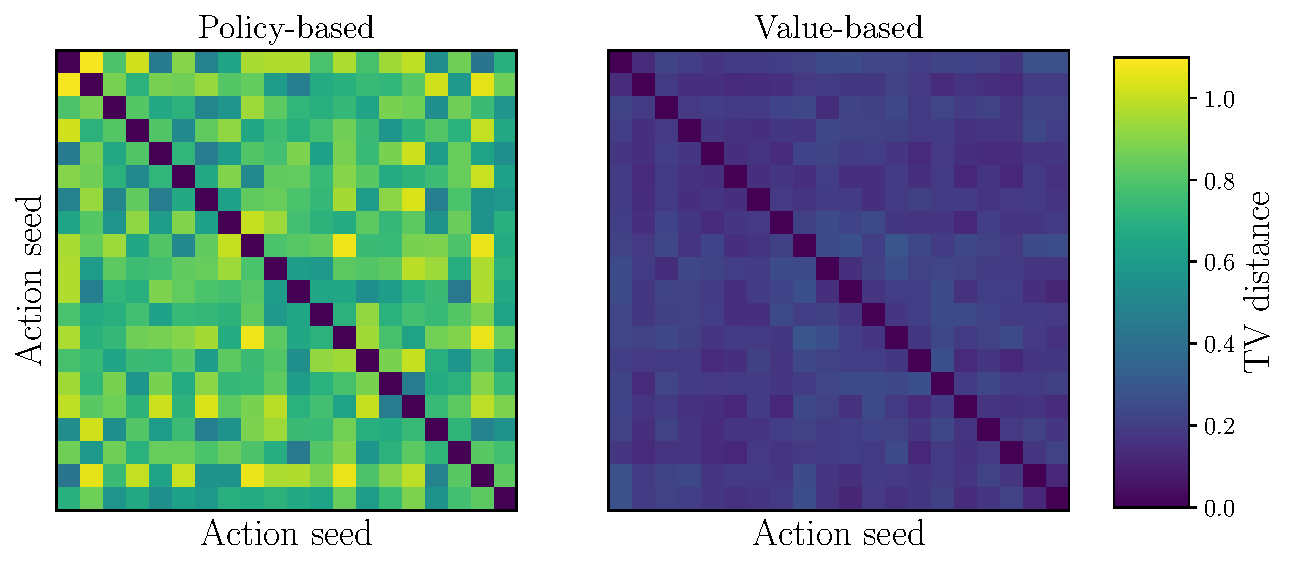
\includegraphics[width=0.48\textwidth]{figures/offline-bandits/toy_stability.pdf}
    \caption{We test action-stability by resampling the actions 20 times for a single dataset of contexts. Each pixel corresponds to the pair of action seeds $ i,j $ and the color shows the TV distance between $ \pi_i(\cdot|x)$ and $ \pi_j(\cdot|x) $ on a held-out test set sampled from the data generating distribution. The policy-based algorithms are highly sensitive to the randomly sampled actions.}
    \label{fig:toy_stability}
\end{figure}


To confirm (1) and (2) listed above we conduct two experiments. First, to test the action-stability of an algorithm with a neural network model, we train 20 different policies on the same dataset of contexts and rewards, but with resampled actions. Formally, we sample $ \{x_i, r_i\}_{i=1}^N$ from the Gaussian distributions described above and then sample $ a_i \sim \beta(\cdot|x_i)$ with 20 different seeds. We then train each algorithm to convergence and compare the resulting policies by total variation (TV) distance. Results are shown in Figure \ref{fig:toy_stability}. We find that our results from Section \ref{sec:stable} are confirmed: policy-based algorithms are unstable leading to high TV distance between policies trained on different seeds while value-based algorithms are stable.


\begin{figure}
    \centering
    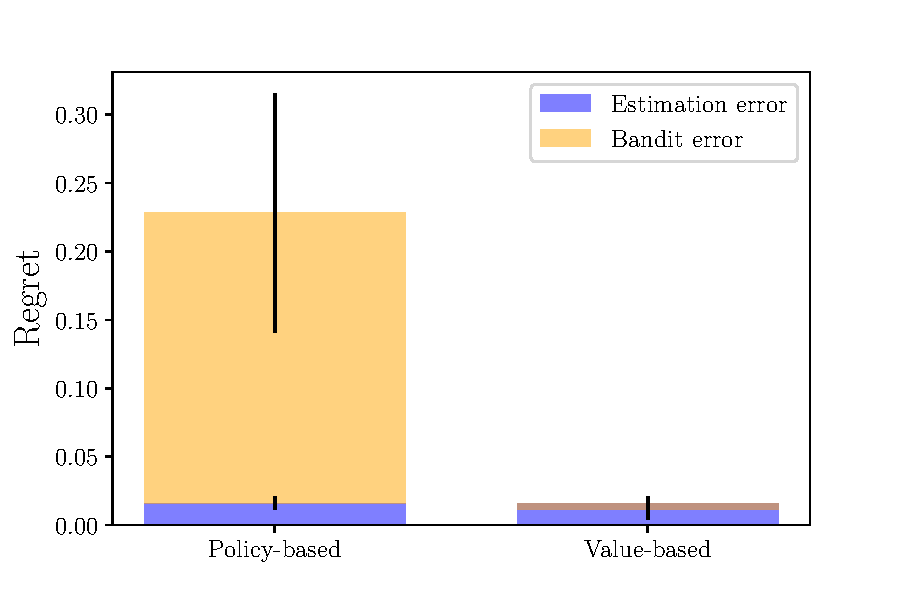
\includegraphics[width=0.3\textwidth]{figures/offline-bandits/toy_regret_bar.pdf}
    \caption{Estimated bandit error by averaging the values calculated on the held-out test sets for 50 independently sampled datasets. Error bars show one standard deviation. While policy-based learning has high bandit error, value-based learning has essentially zero bandit error.}
    \label{fig:toy_regret}
\end{figure}


Second, we estimate the bandit error of each algorithm. To do this we train policies to convergence for the policy-based, value-based, and full-feedback objectives 50 independently sampled datasets (where now we also resample the contexts and rewards). For this estimate, we assume perfect optimization and no approximation error. Each estimate is calculated on a held out test set. Explicitly, let $ \pi_B^j, \pi_Q^j, \pi_F^j$ are the policy-based, value-based, and full-feedback policies trained on dataset $ S^j$ with seed $ j$ and corresponding test set $ T^j$. Then we estimate bandit error as $ \frac{1}{J}\sum_{j=1}^J V(\pi_F^j;T^j) - V(\pi_B^j; T^j)$. Similarly, since we know $ \theta$ we can compute $ \pi^*$ and use this to estimate the estimation error. The results shown in Figure \ref{fig:toy_regret} demonstrate that the policy-based algorithm suffers from substantially more bandit error and thus more regret.


\subsection{Classification data}

Most prior work on offline contextual bandits conducts experiments on classification datasets that are transformed into bandit problems \cite{beygelzimer2009offset, dudik2011doubly, swaminathan2015counterfactual, swaminathan2015self, joachims2018deep, chen2019surrogate}. This methodology obscures issues of action-stability because the very particular reward function used (namely 1 for a correct label and 0 for incorrect) makes the policy-based objective action-stable. However, even minor changes to this reward function can dramatically change the performance of policy-based algorithms by rendering the objective action-unstable.

To make a clear comparison to prior work that uses deep neural networks for offline contextual bandits like \citet{joachims2018deep}, we will consider the same image based bandit problem that they do in their work. Namely, we will use the a bandit version of CIFAR-10 \citep{Krizhevsky09learningmultiple}.

To turn CIFAR into an offline bandit problem we view each possible label as an action and assign reward of 1 for a correct label/action and 0 for an incorrect label/action. We use two different behavior policies to generate training data: (1) a uniformly random behavior policy and (2) the hand-crafted policy used in \citep{joachims2018deep}. We train Resnet-18 \citep{he2016deep} models using Pytorch \citep{paszke2019pytorch}. Again full details about the training procedure are in Appendix \ref{app:experiments}.

As explained in Section \ref{sec:stable}, the policy-based objective is stable if and only if the sign of the reward minus baseline is an indicator of the optimal action. To test this insight we consider two variants of policy-based learning: ``unstable'' where we use a baseline of -0.1 so that the effective rewards are 1.1 for a correct label and 0.1 for incorrect and ``stable'' where we use a baseline of 0.1 so that the effective rewards are of 0.9 and -0.1 to make the objective stable\endnote{This corresponds to the optimal value of $ \lambda$ in the experiments of \citet{joachims2018deep}. Our ``stable'' model slightly outperforms theirs, likely due to a slightly better implementation.}. Note that this ``stable'' variant of the algorithm \emph{only} exists because we are considering a classification problem. In settings with more rich structure in the rewards, defining such an algorithm is not possible and only versions of the unstable algorithm would exist.

\begin{figure}
    \centering
    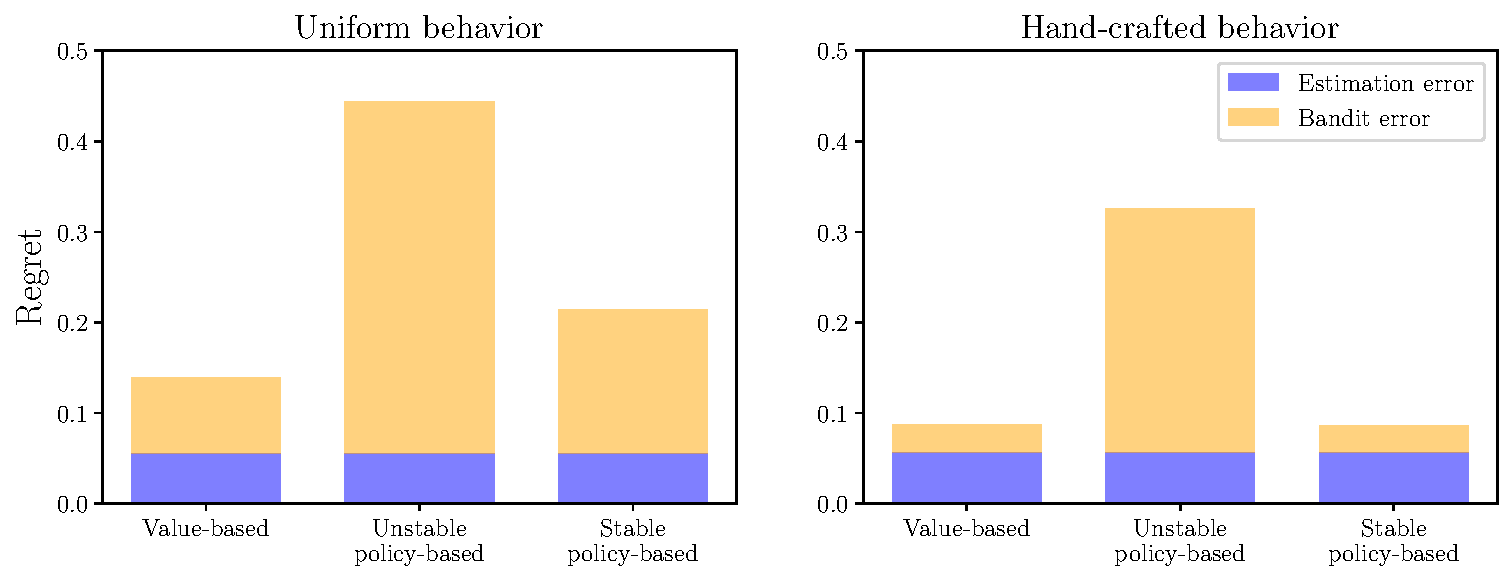
\includegraphics[width=0.48\textwidth]{figures/offline-bandits/cifar_regret_bar.pdf}
    \caption{Estimated regret decomposition on CIFAR with uniform behavior (left) and the hand-crafted behavior of \citet{joachims2018deep} (right). We see that the value-based learning has lowest bandit error and unstable policy-based learning the most. On the hand-crafted dataset the stable policy-based algorithm performs as well as value-based learning.}
    \label{fig:cifar_regret}
\end{figure}

We again estimate the regret decomposition as we did with the synthetic data. The difference is that this time we only use one seed since we only have one CIFAR-10 dataset. The results in Figure \ref{fig:cifar_regret} confirm the results from the synthetic data. The standard (unstable) policy-based algorithm suffers from large bandit error. The value-based algorithm has the best performance across both datasets although the ``stable'' policy-based algorithm performs about as well for the hand-crafted behavior policy.

\section{Related work}\label{sec:related}

Now that we have presented our results, we will contrast them with some related work to clarify our contribution.

\subsection{Relation to propensity overfitting}
\citet{swaminathan2015self} introduce what they call ``propensity overfitting''. By providing an example, they show that policy-based algorithms overfit to maximize the sum of propensities $( \sum_i \frac{\pi(a_i|x_i)}{p_i})$ rather than the value when the rewards are strictly positive. They provide a motivating example, but no formal definition of propensity overfitting and argue that it helps to describe the gap between supervised learning and bandit learning. In contrast, we introduce and formally define bandit error, which makes this gap between supervised learning and bandit learning precise and does not rely on the specific algorithm being used. Then we introduce and formally define action-instability, which explains an important cause of bandit error for policy-based algorithms when using large models.
By mathematically formalizing these ideas we provide a more rigorous foundation for future work.

\subsection{Relation to \cite{joachims2018deep}}

The main related work that considers offline contextual bandits with large neural network models is \citet{joachims2018deep}. Specifically, that paper proposes a policy-based algorithm with an objective of the form: $\frac{r_i(a_i) - \lambda}{\beta(a_i|x_i)} \pi(a_i|x_i)$ for some constant baseline $ \lambda$ determined by a hyperparameter sweep, but motivated by a connection to self-normalized importance sampling.

Our work contrasts with this prior work in two key ways. First, we show that the algorithm proposed in \citet{joachims2018deep} is action-unstable. Specifically, our Lemma \ref{lem:pb-stable} shows that any policy-based algorithm with an objective of the form $ \sum_i f(z_i(a_i)) \pi(a_i|x_i)$ cannot be action-stable unless the sign of $ f(z(a))$ is the indicator of the optimal action. However, since that paper only tests the algorithm on classification problems where the rewards are in $ \{0,1\}$, any setting of $ \lambda$ between 0 and 1 causes the sign of $ f $ to indicate the optimal action. The action-stability analysis shows how this algorithm will struggle beyond the classification setting.

Second, we show that value-based methods provably and empirically work in the overparameterized setting. In contrast, \citet{joachims2018deep} does not consider value-based methods. We show that value-based methods are not affected by action-stability issues (Lemma~\ref{lem:vb-stable}) and have vanishing bandit error (Theorem \ref{thm:reduction}). We empirically test this conclusion on the same CIFAR-10 bandit problem as \citet{joachims2018deep} and find that a value-based approach outperforms the policy-based approach proposed in that paper (Figure \ref{fig:cifar_regret}).

\subsection{Variance of importance weighting}

The importance weighted value estimates used by policy-based algorithms suffer from high variance due to low probability actions that have very large importance weights.
Much prior work focuses on reducing this variance \cite{strehl2010learning, bottou2013counterfactual, swaminathan2015counterfactual}.
In contrast, the issue we consider, action-instability in the overparameterized setting, is distinct from this variance issue.
When the policy class is flexible enough to optimize the objective at each datapoint, the optimal predictor in that class does not depend on the importance weights.
Meanwhile action-unstable objectives translate stochasticity in the behavior policy into noise in the objective, causing the overfitting issues that we see in policy-based algorithms.
In fact, our Theorem~\ref{thm:vs} suggests that regret will be worse for more uniform behavior policies when using an action-unstable objective, even though these may be beneficial in terms of variance.
This is born out in our experiments where the behavior is usually \emph{uniform} and \emph{known}, which is a favorable setup in terms of the variance of the value estimates, but an unfavorable setup for action-unstable policy learning algorithms.


\section{Discussion}
We have examined the offline contextual bandit problem with overparameterized models. We introduced a new regret decomposition to separate the effects of estimation error and bandit error. We showed that policy-based algorithms are not action-stable and thus suffer from high bandit error with stochastic behavior policies.
This is borne out both in the theory and experiments.

It is important to emphasize that our results may not apply beyond the setting we consider in this paper. When there is no strict positivity, there is unobserved confounding, there are continuous actions, or the model classes are small and misspecified then policy-based learning may have lower regret and lower bandit error than value-based learning.

In future work we hope to extend the ideas from the bandit setting to the full RL problem with longer horizon that requires temporal credit assignment. We predict that action-stability and bandit error remain significant issues there.
We also hope to investigate action-stable algorithms beyond the simple value-based algorithms we consider here.
%We also hope to leverage some of the theoretical understanding from this paper into algorithmic improvements to combat bandit overfitting.






\clearpage
\begin{subappendices}
\newappendix{Action-stability}\label{app:stable}

\vbstable*

\begin{proof}
Consider a datapoint $ z= (x,r)$ which becomes $ z(a) = (x, a, r(a))$ when we sample action $ a$ from the behavior. At this datapoint, the value-based objective for an estimated Q function $ \hat Q$ is
\begin{align}
    \ell(z(a), \hat Q(x, a)) = (r(a) - \hat Q(x,a))^2
\end{align}
This is minimized at all $ a $ by $\hat Q(x,a) = r(a)$. So setting $ y^* = \hat Q(x, \cdot) = r$, we can exactly minimize $ \ell$ at $ z$. Since such a $ y^*$ exists, the objective is by definition action-stable.
\end{proof}



\pbstable*

\begin{proof}
Consider a datapoint $ z= (x,r)$ which becomes $ z(a) = (x, a, r(a), p(a))$ when we sample action $ a$ from the behavior with probability $ p(a)$. At this datapoint, a generic policy-based objective evaluated on a policy $ \hat \pi $ takes the form
\begin{align}
    \ell(z(a), \hat \pi(a|x)) = f(z(a)) \hat \pi(a|x)
\end{align}
As special examples of the function $ f $ we have the generic policy-based objective from Equation (\ref{eq:pi}) when $ f(z(a)) = \frac{r(a)}{p(a)}$. Moreover we can incorporate any baseline function $ b(x)$ so that $ f(z(a)) = \frac{r(a) - b(x)}{p(a)}$. This algorithm covers the one presented by \citet{joachims2018deep}.

Now to prove the claim, we have three cases: (1) $ f(z(a)) < 0$ for all $ a$, (2) $ f(z(a)) > 0 $ for at least two actions $ a_1, a_2$, and (3) $ f(z(a)) > 0$ at exactly one action $ a_1$. We will show that in cases 1 and 2 the objective is action-unstable, but in case 3 it is action-stable.

\paragraph{Case 1.} Assume that $ f(z(a)) < 0$ for all $ a$. Now for any given $ a $ to maximize the objective $f(z(a))\hat \pi(a|x)$ while ensuring that $ \hat \pi(a|x) $ is a valid probability we must set $ \hat \pi(a|x) = 0$. But, if we set $ \hat\pi(a|x) = 0$ for all $ a$, we no longer have a valid probability distribution, since $ 0 \not \in \Delta^K$. Thus, we cannot find $ y^* \in \Delta^K$ that optimizes the loss at $ z $ across all actions, so the objective is action-unstable.

\paragraph{Case 2.} Assume that $ f(z(a)) > 0 $ for at least two actions $ a_1, a_2$. Now at $ a_1, a_2$ the objective $f(z(a))\hat \pi(a|x)$ is maximized by setting $ \pi(a|x) = 1$. However, there is no valid element $ y $ of $ \Delta^K$ such that $ y(a_1) = 1$ and $y(a_2) = 1$. Thus, we cannot find $ y^* \in \Delta^K$ that optimizes the loss at $ z $ across all actions, so the objective is action-unstable.

\paragraph{Case 3.} Assume $f(z(a)) > 0$ at exactly one action $ a_1$. Then at action $ a_1$ we can maximize $ f(z(a_1))\hat \pi(a_1|x)$ by setting $ \hat\pi(a_1|x) = 1$. And since $ f(z(a)) \leq 0$ for all other actions $ a \neq a_1$, we can maximize $ f(z(a))\hat \pi(a|x)$ by setting $ \hat\pi(a|x) = 0$. Now since $ \one[a = a_1] \in \Delta^K$, there does exist a vector $ y^* \in \mathcal{Y}$ which exactly optimizes $ \ell$ regardless of which action is sampled. So, the objective is action-stable if and only if we are in this case.
\end{proof}




\newappendix{Value-based learning}\label{app:value}

\reduction*

\begin{proof}
The proof follows directly from linking the subsequent lemmas with $ \hat \pi = \pi_{\hat Q_{S_B}}$ and $ \Pi$ be the set of all policies in Lemma \ref{lem:mismatch}.
\end{proof}


% \paragraph{Mismatch.} We need to connect the bound on worst case the regression error to the value of the learned policy. This follows from some algebraic manipulation and an application of Jensen's inequality and is encoded in the following Lemma.

\begin{restatable}[Mismatch: from MSE to Regret]{lemma}{mismatch}\label{lem:mismatch}
Assume strict positivity. Let $\hat \pi$ be the greedy policy with respect to some $ \hat Q $ and let $ \Pi$ be any class of policies to compete against, which contains $ \hat \pi$. Then
\begin{align}
    \sup_{\pi\in \Pi} V(\pi) - V(\hat\pi) \leq 2 \sqrt{\sup_{\pi\in \Pi} \E_{x,a \sim \mathcal{D}, \pi}[ (Q(x,a) - \hat Q(x,a))^2]}
\end{align}
\end{restatable}


\begin{proof}
We can expand the definition of regret and then add and subtract and apply a few inequalities. Let $ \bar \pi $ be the policy in $ \Pi $ which maximizes $ V$. Then
\begin{align}
    \sup_{\pi\in \Pi}V(\pi) - V(\hat \pi) &=  \E_x\bigg[\E_{a\sim \bar\pi|x}[Q(x,a)] - \E_{a\sim\hat\pi|x}[Q(x,a)]\bigg]\\
    &= \E_x\bigg[\E_{a\sim \bar\pi|x}[ Q(x,a)] - \E_{a\sim\hat\pi|x}[\hat Q(x,a)] + \E_{a\sim\hat\pi|x}[\hat Q(x,a)] - \E_{a\sim\hat\pi|x}[Q(x,a)]\bigg]\\
    &\leq \E_x\bigg[\E_{a\sim \bar\pi|x}[| Q(x,a) -\hat Q(x,a)|] + \E_{a\sim\hat\pi|x}[|Q(x,a)-\hat Q(x,a)|]\bigg]\\
    &\leq \sqrt{\E_x\E_{a\sim \bar\pi|x}[(Q(x,a) -\hat Q(x,a))^2]} + \sqrt{\E_x\E_{a\sim \hat\pi|x}[(Q(x,a) -\hat Q(x,a))^2]} \\
    &\leq 2  \sqrt{ \sup_{\pi\in \Pi}\E_x\big[\E_{a\sim \pi|x}[(Q(x,a)-  \hat Q(x,a))^2]\big]}
\end{align}
The first inequality holds since $ \hat \pi $ maximizes $ \hat Q$ and by using the definition of absolute value, the second by Jensen, and the third by introducing the supremum.
\end{proof}

\begin{restatable}[Transfer: from $\beta$ to $\pi$]{lemma}{transfer}\label{lem:transfer}
Assume strict positivity and take any Q-function $ \hat Q $ and any policy $ \pi$, then
\begin{align}
    \E_{x, a\sim \mathcal{D}, \pi}[Q(x,a) - \hat Q(x,a))^2] < \frac{1}{\tau}\bigg(\E_{x,a \sim \mathcal{D}, \beta}[(Q(x,a) - \hat Q(x,a))^2]\bigg).
\end{align}
\end{restatable}
\begin{proof} Let $ \pi$ be any policy. Then
\begin{align}
    \E_{x}\E_{a\sim \pi|x} [(Q(x,a) - \hat Q(x,a))^2] &=  \int_x p(x) \sum_a \pi(a|x) (Q(x,a) - \hat Q(x,a))^2 dx \\
    &=  \int_x \sum_a \pi(a|x) \frac{\beta(a|x)}{\beta(a|x)} p(x) (Q(x,a) - \hat Q(x,a))^2 dx \\
    &<  \frac{1}{\tau}\int_x \sum_a \beta(a|x) p(x) (Q(x,a) - \hat Q(x,a))^2 dx\\
    &= \frac{1}{\tau} \E_{x,a \sim \mathcal{D}, \beta}[(Q(x,a) - \hat Q(x,a))^2]
\end{align}
where we use a multiply and divide trick and apply the definition of strict positivity to ensure that $ \frac{\pi(a|x)}{\beta(a|x)} < \frac{1}{\tau}$.
\end{proof}


\newappendix{Policy-based learning}\label{app:pb}


\subsection{In-sample regret}



\begin{lemma}\label{lem:policy_decomp}
Let $ \Pi$ be an interpolating class and $ K = 2$. Then there exists a $ \pi_B $ as defined in Equation (\ref{eq:pi}) such that
\begin{enumerate}
    \item the behavior of $ \pi_B$ at each datapoint $ x_i \in S$ only depends on $ a_i, r_i(a_i)$, and $ p_i$
    \item $ \pi_B(\cdot|x_i) \in \{(0,1),(1,0)\}$.
\end{enumerate}
\end{lemma}
\begin{proof}
We will begin by proving part 2. Note that the objective that $ \pi_B$ optimizes takes the form $ \frac{r_i(a_i)}{p_i}\pi(a_i|x_i)$ at each datapoint. Since probabilities are constrained to $[0,1]$ this is optimized by $ \pi(a_i|x_i) = 0$ if $ \frac{r_i(a_i)}{p_i} < 0$ and $ \pi(a_i|x_i) = 1$ if $ \frac{r_i(a_i)}{p_i} > 0$. Since we have an overparameterized model class, we know that $ \Pi$ contains a $ \pi_B$ that can exactly choose the optimizer at each datapoint. Since $ K=2$, once we know $ \pi(a_i|x_i)$ we immediately have $ \pi(\bar a_i|x_i) = 1 - \pi(a_i|x_i)$ (where $ \hat a_i$ is the action that is not equal to $ a_i$). Thus $ \pi_B(\cdot|x_i) \in \{(0,1),(1,0)\}$.

Now part 1 follows directly since the above reasoning showed that $ \pi_B(\cdot|x_i)$ is defined precisely by the sign of $ \frac{r_i(a_i)}{p_i}$ and the identity of $ a_i$.
\end{proof}



\vsthm*

\begin{proof}
By part 1 of Lemma \ref{lem:policy_decomp} and linearity of expectation we can decompose the expected in-sample value as
\begin{align*}
    \E_{S}[V(\pi^*;S) - V(\pi_B;S)] = \frac{1}{N}\sum_{i=1}^N \E_{x_i, r_i, a_i}\bigg[ \E_{a\sim \pi^*}\E_{r|x_i}[r(a)] -  \E_{a\sim \pi_B}\E_{r|x_i}[r(a)]\bigg].
\end{align*}

Since the data are iid we further have that
\begin{align*}
    \E_{S}[V(\pi^*;S) - V(\pi_B;S)] = \E_{x_i, r_i, a_i}\bigg[ \E_{a\sim \pi^*}\E_{r|x_i}[r(a)] -  \E_{a\sim \pi_B}\E_{r|x_i}[r(a)]\bigg].
\end{align*}

Define the event $ U_{x,r}$ to be the event that the policy-based objective is action-unstable at $ x,r$. So $ p_u(x) = \E_{r|x}[\one[U_{x,r}]]$.
We can split this expectation up into stable and unstable parts by conditioning on either $ \overline U_{x_i, r_i}$ or $ U_{x_i, r_i}$, and lower bound the regret on the stable datapoints by 0:
\begin{align*}
    \E_{S}[V(\pi^*;S) - V(\pi_B;S)] &= \E_{x_i, r_i |\overline U_{x_i, r_i}} \E_{a_i|x_i}\bigg[ \E_{a\sim \pi^*}\E_{r|x_i}[r(a)] -  \E_{a\sim \pi_B}\E_{r|x_i}[r(a)]\bigg] \\
    &\qquad + \E_{x_i, r_i |U_{x_i, r_i}} \E_{ a_i|x_i}\bigg[ \E_{a\sim \pi^*}\E_{r|x_i}[r(a)] -  \E_{a\sim \pi_B}\E_{r|x_i}[r(a)]\bigg]\\
    &\geq \E_{x_i, r_i |U_{x_i, r_i}} \E_{ a_i|x_i}\bigg[ \E_{a\sim \pi^*}\E_{r|x_i}[r(a)] -  \E_{a\sim \pi_B}\E_{r|x_i}[r(a)]\bigg].
\end{align*}

By part 2 of Lemma \ref{lem:policy_decomp} we know that $ \pi_B(\cdot|x_i) $ is either $ (1,0)$ or $ (0,1)$. Conditioned on the objective being unstable at $ x_i$ and using the fact that there are only two actions, we know that $ \pi_B(x_i)$ must be different depending on whether $ a_i = 1$ or $ a_i = 2$. Define $ a_{i,B}^1$ to be the action that $ \pi_B$ selects at $ x_i $ when $ a_i = 1$ and $ a_{i,B}^2$ the action when $ a_i = 2$.
Let $ a_i^*$ be the action chosen by the deterministic optimal policy $ \pi^*$ at $ x_i$.
Thus we can split the expectation over $ a_i$ in the above expression and then plug in definitions to get:
\begin{align*}
    \E_{S}[V(\pi^*;S) - V(\pi_B;S)] &\geq \E_{x_i, r_i |U_{x_i, r_i}} \bigg[\beta(a_i = 1|x_i) \E_{r|x_i}[r(a^*_i) - r(a_{i,B}^1)] + \beta(a_i = 2|x_i) \E_{r|x_i}[r(a^*_i) - r(a_{i,B}^2)]\bigg].
\end{align*}
Since we assumed that $ \beta (a|x_i) \geq \tau$ for all $ a$ we can lower bound the above by
\begin{align*}
    \E_{S}[V(\pi^*;S) - V(\pi_B;S)] &\geq \tau \E_{x_i, r_i} \bigg[\one[U_{x_i, r_i}]\bigg( \E_{r|x_i}[r(a_i^*) - r(a_{i,B}^1)] +  \E_{r|x_i}[r(a_i^*) - r(a_{i,B}^2)]\bigg)\bigg].
\end{align*}
Finally, we note that since $ a_{i,B}^1 \neq a_{i,B}^2$ and there are only 2 actions that the above is precisely
\begin{align*}
    \E_{S}[V(\pi^*;S) - V(\pi_B;S)] &\geq  \tau \E_{x_i, r_i} \bigg[\one[\overline E_{x_i, r_i}] \E_{r|x_i}[r(a_i^*) - r(a \neq a^*_i)]\bigg]\\
    &= \tau \E_{x_i, r_i} [\one[\overline E_{x_i, r_i}] \Delta_r(x_i)]\\
    &= \tau \E_{x_i} [\E_{r_i|x_i}[\one[U_{x_i, r_i}]] \Delta_r(x_i)]\\
    &= \tau \E_{x_i} [p_u(x_i) \Delta_r(x_i)]\\
    &= \tau \E_{x} [p_u(x) \Delta_r(x)].
\end{align*}
\end{proof}



\subsection{Connection to noisy classification}\label{app:noisy}

This section states and proves the Theorem referenced in the main text connecting action-unstable policy-based learning with noisy classification.

%\noisy*
\begin{restatable}[Noisy classification reduction]{theorem}{noisy}\label{thm:noisy}
Take any noise level $ \eta < 1/2$ and any binary classification problem $ \mathcal{C}$ consisting of a distribution $\mathcal{D}_\mathcal{C}$ over $ \mathcal{X}$ and a labeling function $ y_{\mathcal{C}}: \mathcal{X} \to \{-1,1\}$.
There exists an offline contextual bandit problem $ \mathcal{B}$ with noiseless rewards such that
\begin{enumerate}
    \item Maximizing $ \hat V_B$ in $\mathcal{B}$ is equivalent to minimizing the 0/1 loss on a training set drawn from $ \mathcal{C}$ where labels are flipped with probability $ \eta$.
    \item Maximizing $ \hat V_F$ in $\mathcal{B}$ is equivalent to minimizing the 0/1 loss on a training set drawn from $ \mathcal{C}$ with noiseless training labels.
\end{enumerate}
\end{restatable}

\begin{proof}
First we will construct the bandit problem $ \mathcal{B}$ with two actions corresponding to the classification problem $ \mathcal{C}$.
For any constant $ c_r > 0 $ we define $ \mathcal{B}$ by
\begin{align}
    x \sim \mathcal{D}_{\mathcal{C}}, \qquad r|x = \begin{cases}c_r(1-\eta, \eta) & y_\mathcal{C}(x) = 1\\ c_r(\eta, 1-\eta) & y_\mathcal{C}(x) = -1\end{cases}, \qquad \beta(1|x) = \begin{cases}1-\eta & y_\mathcal{C}(x) = 1\\ \eta & y_\mathcal{C}(x) = -1\end{cases}
\end{align}
Now we will show that in this problem, $ \hat V_B$ is equivalent to the 0/1 loss for $ \mathcal{C}$ with noisy labels. To do this first note that by construction, for $ x $ with $ y_\mathcal{C}(x) = 1$ we have $ \frac{r(1)|x}{\beta(1|x)} = \frac{c_r(1-\eta)}{1-\eta} = c_r$ and $ \frac{r(2)|x}{\beta(2|x)} = \frac{c_r\eta}{\eta} = c_r$, and similarly for $ x $ with $ y_\mathcal{C}(x) = -1$ we have $ \frac{r(1)|x}{\beta(1|x)} = \frac{c_r\eta}{\eta} = c_r$ and $ \frac{r(2)|x}{\beta(2|x)} = \frac{c_r(1-\eta)}{1-\eta} = c_r$.
\begin{align}
    \hat V_B(\pi) &= \frac{1}{N} \sum_{i=1}^N r_i(a_i) \frac{\pi(a_i|x_i)}{\beta(a_i|x_i)} = \frac{1}{N} \sum_{i=1}^N  \frac{r_i(a_i)}{\beta(a_i|x_i)} \pi(a_i|x_i) \\
    &= \frac{c_r}{N} \sum_{i=1}^N  \pi(a_i|x_i)
\end{align}
This is equivalent to 0/1 loss with noisy labels since $ \beta$ generates $ a_i$ according to $ y_\mathcal{C}$ where the label is flipped with probability $ \eta$.

Now we will show that $ \hat V_F$ is equivalent to the 0/1 loss for $ \mathcal{C}$ with clean labels. Note that by construction $ r(a)|x = c_r \eta + \pi^*(a|x)c_r (1 - 2 \eta)$. So,
\begin{align}
    \hat V_F(\pi) &= \frac{1}{N} \sum_{i=1}^N \langle r_i, \pi(\cdot|x_i)\rangle = \frac{c_r}{N} \sum_{i=1}^N \langle \eta \textbf{1} + (1 - 2\eta) \pi^*(\cdot|x_i), \pi(\cdot|x_i)\rangle \\
    &= \frac{c_r \eta}{N} +  \frac{c_r (1 - 2\eta)}{N} \sum_{i=1}^N \langle  \pi^*(\cdot|x_i), \pi(\cdot|x_i)\rangle
\end{align}
This is equivalent to 0/1 loss with noisy labels since $ \pi^*$ exactly corresponds to $ y_\mathcal{C}$.
\end{proof}





\subsection{Nearest Neighbor}

\nn*

\begin{proof}
First we need to formally define the nearest neighbor rules that interpolate the objectives $ \hat V_B$ and $ \hat V_F$. These are simple in the case of two actions. Let $ i(x)$ be the index of the nearest neighbor to $ x$ in the dataset. Then
\begin{align}
    \pi_B(a|x) = \begin{cases}1 & \big(a = a_{i(x)} \ \textsc{and}\  r_{i(x)}(a_{i(x)}) > 0\big) \textsc{or} \big(a \neq a_{i(x)} \ \textsc{and}\  r_{i(x)}(a_{i(x)}) \leq 0\big) \\ 0 & otherwise.\end{cases}
\end{align}
This is saying that $ \pi_B$ chooses the same action as the observed nearest neighbor if that reward was positive, and the opposite action if that was negative.
And for the full feedback we just choose the best action from the nearest datapoint.
\begin{align}
    \pi_F(a|x) = \begin{cases}1 & a = \arg\max_{a'} r_{i(x)}(a')\\ 0 & otherwise. \end{cases}
\end{align}

Now we can construct the problem instances needed for the Theorem.
To construct the example, take a bandit problem with two actions (called 1 and 2):
\begin{align*}
    x \sim U([-1,1]), \quad r|x = (1, 1 + \Delta_r), \quad \beta(1|x) = \beta(2|x) = 1/2 \ \forall\ x,a
\end{align*}
The true optimal policy has $\pi^*(2|x) = 1$ for all $x$ and $ V(\pi^*) = 1+\Delta_r$.
The policy with full feedback $ \pi_F $ is to always choose action 2, since every observation will show that action 2 is better.


Now, we will show that in the limit of infinite data, $ \pi_F$ has no regret. Since the rewards are noiseless, the maximum observed reward at a context is exactly the optimal action at that context. Thus, we precisely have a classification problem with noiseless labels so that the Bayes risk is 0.
Since we $\pi^*$ is continuous, the class conditional densities (determined by the indicator of the argmax of $ Q$) are piecewise continuous.
This allows us to apply the classic result of \cite{cover1967} that a nearest neighbor rule has asymptotic risk less twice the Bayes risk, which in this case is zero. This means that asymptotically $ P(\pi_F(a|x) \neq \pi^*(a|x)) = 0$ which immediately gives the second desired result of zero regret in the limit of infinite data under full feedback.

Now we note that since rewards are always positive, we can simplify the definition of $ \pi_B$ as
\begin{align}
    \pi_{B}(a|x) = \one[a = a_{i(x)}].
\end{align}

Then we have that
\begin{align}
    V(\pi_F) - V(\pi_{B}) &= \E_x [\E_{a\sim \pi_F|x}[Q(x,a)] - \E_{a\sim \pi_{B}|x}[Q(x,a)] ]\\
    &= \E_x [\Delta_r + 1 - (\pi_{B}(1|x) + \pi_{B}(2|x) (\Delta_r + 1))] ] \\
    &= \Delta_r + 1 - \E_x[\one[a_{i(x)} = 1] + (\Delta_r + 1)\one[a_{i(x)} = 2]]
\end{align}
Taking expectation over $ S$ we get
\begin{align}
    \E_S[V(\pi_F) - V(\pi_{B})] &= \E_S[\Delta_r + 1 - \E_x[\one[a_{i(x)} = 1] + (\Delta_r + 1)\one[a_{i(x)} = 2]]]\\
    &= \Delta_r + 1 - \E_x[P_S(a_{i(x)} = 1) + (\Delta_r + 1)P_S(a_{i(x)} = 2)]]\\
    &= \Delta_r + 1 - \E_x[\frac{1}{2} + (\Delta_r + 1)\frac{1}{2}]]\\
    &= \frac{\Delta_r}{2}
\end{align}
This construction did not depend on the size of the dataset, so it is even true as the number of datapoints tends to infinity.
\end{proof}



\newappendix{Discussion of doubly robust algorithms}\label{app:dr}


Before going into the comparison, we will define the doubly robust algorithm \cite{dudik2011doubly} in our notation. Specifically,
\begin{align}\label{eq:dr}
    \widehat V_{DR} (\pi) := \sum_{i=1}^N \bigg[ \sum_a \pi(a|x_i) \hat Q(x_i, a) + \frac{\pi(a_i|x_i)}{\beta(a_i|x_i)} (r_i(a_i) - \hat Q(x_i, a_i)) \bigg], \qquad \hat \pi_{DR} = \arg\max_{\pi \in \Pi} \widehat V_{DR}(\pi)
\end{align}

As stated in the main text, when we use overparameterized models and train $ \hat Q$ on the same data that we use to optimize the policy, then doubly robust methods are equivalent to the vanilla value-based algorithm. This is formalized in Lemma \ref{lem:dr_equiv} below.

This equivalence can be avoided by using crossfitting so that $ \hat Q$ is not trained on the same data as $ \pi$. However, then it is possible that the doubly robust policy objective becomes action-unstable. This is true \emph{even with} access to the true $Q$ function, but requires stochastic rewards. To construct such an example we leverage the stochastic rewards so that instability only occurs at datapoints where certain reward vectors are sampled. This is shown in Lemma \ref{lem:dr_unstable} below.

One final point is to consider the motivation for doubly robust methods. Usually it is motivated by concerns about consistency of the value function estimation or estimation of behavior policy \cite{dudik2011doubly}. However, in our setting we have (1) an overparamterized model class which is large enough to contain the true value function, and (2) exact access to the behavior probabilities. So it is not clear why doubly robust methods would be motivated in our setting.

\begin{lemma}[Equivalence of DR and vanilla VB]\label{lem:dr_equiv}
When we use overparameterized models and do not use crossfitting, doubly robust learning from Equation (\ref{eq:dr}) is equivalent to vanilla value-based learning from Equation (\ref{eqn:hatQ}).
\end{lemma}

\begin{proof}
When the model for $ \hat Q$ is overparameterized and trained on the full dataset, we know that $ \hat Q(x_i, a_i) = r_i(a_i)$. Thus we get that
\begin{align}
    \widehat V_{DR} (\pi) &= \sum_{i=1}^N \bigg[ \sum_a \pi(a|x_i) \hat Q(x_i, a) + \frac{\pi(a_i|x_i)}{\beta(a_i|x_i)} (r_i(a_i) - \hat Q(x_i, a_i)) \bigg]\\
    &= \sum_{i=1}^N \bigg[ \sum_a \pi(a|x_i) \hat Q(x_i, a) + \frac{\pi(a_i|x_i)}{\beta(a_i|x_i)} (0) \bigg]\\
    &= \sum_{i=1}^N \sum_a \pi(a|x_i) \hat Q(x_i, a)
\end{align}
With an overparameterized policy class, we can exactly recover the greedy policy relative to $ \hat Q$ to optimize this objective.
\end{proof}


\begin{lemma}[Instability of DR]\label{lem:dr_unstable}
There exist problems with stochastic rewards where even with access to the exact Q function, the doubly robust policy objective is action-unstable with probability 1/2.
\end{lemma}

\begin{proof}
We need only consider one datapoint since the action-stability property is defined on a per datapoint basis. To make this construction we will consider only two actions.
\begin{align}
    r|x = \begin{cases} (0, 1) & w.p.\ 1/2\\ (0, -2) & otherwise\end{cases}, \qquad \beta(\cdot|x) = (1/2, 1/2)
\end{align}
So, we know that
\begin{align}
    Q(\cdot|x) = (0,-0.5)
\end{align}
Now we claim that when the sampled datapoint has $ r = (0,1)$ the doubly robust objective is action-unstable (and this happens with probability 1/2 by construction).
We can explicitly expand the DR objective for the policy $ \pi$ at $ x $ when action $ a $ is sampled
\begin{align}
    \ell_{DR}(\pi, x, a, r) = \pi(1|x) \cdot 0 + \pi(2|x) \cdot (-0.5) + \frac{\pi(a|x)}{1/2}(r(a) - Q(x,a))
\end{align}
So when $a = 1$ we have $ r(a) = 0$ and $ Q(x,a) = 0$ so that
\begin{align}
    \ell_{DR}(\pi, x, a, r) = \pi(2|x) \cdot (-0.5) + 2 \cdot \pi(1|x)(0 - 0) = \pi(2|x) \cdot (-0.5)
\end{align}
And when $ a=2$ we have $ r(a) = 1$ (because that was the sampled reward) and $ Q(x,a) = 0$ so that
\begin{align}
    \ell_{DR}(\pi, x, a, r) = \pi(2|x) \cdot (-0.5)  + 2 \cdot \pi(2|x) (1 - (-0.5)) = \pi(2|x) \cdot (2.5)
\end{align}
Now, this is clearly action-unstable since the optimizer when $ a=1 $ is sampled is $ \pi(\cdot|x) = (1,0)$ while when $ a = 2$ is sampled we get $ \pi(\cdot|x) = (0,1)$.
\end{proof}





\newappendix{Details of Bandit Experiments}\label{app:experiments}

\subsection{Synthetic data}

\paragraph{Data.} As described in the main text we sample some hidden reward matrix $ \theta$ and then sample contexts and rewards from isotropic Gaussians:
\begin{align*}
    \theta \sim U([0,1]^{K\times d}),\quad x \sim \mathcal{N}(0, I_d), \quad r \sim \mathcal{N}(\theta x, \epsilon I_d).
\end{align*}
Actions are sampled according to a uniform behavior:
\begin{align*}
    a\sim \beta(\cdot|x) = U(\{1,\dots,K\}).
\end{align*}
We set $ K=2, d = 10, \epsilon = 0.1$. For each random seed we take $ N = 100$ training points and sample an independent test set of 500 points.
For experiment 1 we sample $ \theta$ and one dataset of $ x,r$ tuples, then we sample 20 independent sets of actions. For experiment 2 we sample all parameters separately to construct each of the 50 datasets.

\paragraph{Model.} For policies and Q functions we use a multilayer perceptron with one hidden layer of width 512 and ReLU activations. The only difference between policy and Q architecture is that the policy has a softmax layer on the output so that the output is a probability distribution.

\paragraph{Learning.} We train using SGD with momentum. Learning rate is 0.01, momentum is 0.9, batch size is 10, and weight decay is 0.0001. We train every model for 1000 epochs decreasing the learning rate by a factor of 10 after 200 epochs. This trains well past the point of convergence in our experience.

\begin{figure}[h]
    \centering
    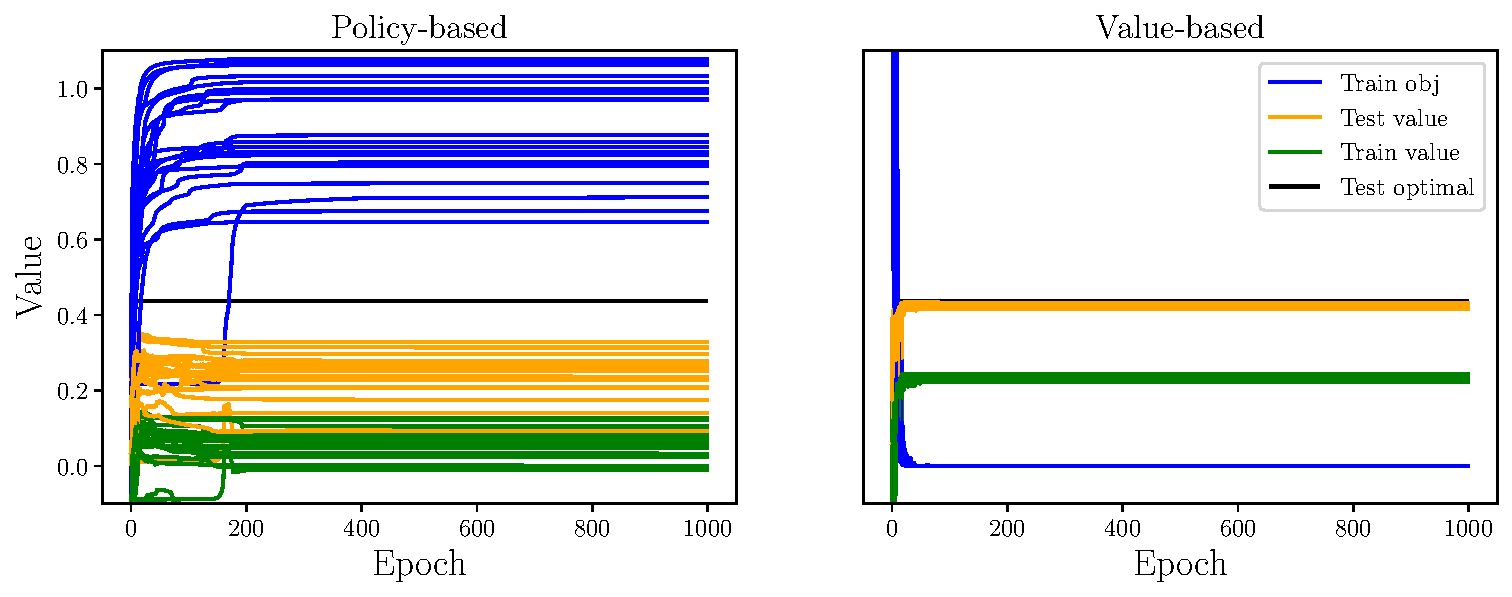
\includegraphics[width=0.7\textwidth]{figures/offline-bandits/toy_learning.pdf}
    \caption{We show learning curves across each of the twenty different action resampled datasets.}
    \label{fig:toy_learning}
\end{figure}

\paragraph{Extended results.}
Figure \ref{fig:toy_learning} shows learning curves for each of the twenty different action datasets from experiment 1. We use ``train obj'' to refer to the training objective which is squared error for value-based learning and $ \hat V_B$ for policy-based learning. We use ``train value'' and ``test value'' to refer to  $ V(\pi;S)$ for $ S$ being the train and test sets respectively. We can evaluate the true value at each datapoint since we know the full reward vector at each datapoint.

We see that the policy-based objective is dramatically higher than the highest achievable value due to overfitting of the noise in the actions. The gap between train and test value is mot likely explained by noise in the contexts sampled in those respective datasets (by chance the test set has higher value contexts).



\subsection{CIFAR-10}

\paragraph{Data.} We use a bandit version of the CIFAR-10 dataset \citep{Krizhevsky09learningmultiple}. We split the train set into a train set of the first 45000 examples and validation set of the last 5000. We normalize the images and use data augmentation of random flips and crops of size 32. Each of the 10 labels becomes an action. We define rewards to be 1 for a correct prediction and 0 for an incorrect prediction.
We use two different behavior policies. One is a uniform behavior that selects each action with probability 0.1 and the other is the hand-crafted behavior policy from \cite{joachims2018deep}.

\paragraph{Model.} We use a ResNet-18 \citep{he2016deep} from PyTorch \citep{paszke2019pytorch} for both the policy and the Q function. The only modification we make to accommodate for the smaller images in CIFAR is to remove the first max-pooling layer.

\paragraph{Learning.} We train using SGD with momentum 0.9,a batch size 128, and weight decay of 0.0001 for 1000 epochs. Training takes about 20 hours for each run on an NVIDIA RTX 2080 Ti GPU. We use a learning rate of 0.1 for the first 200 epochs, 0.01 for the next 200, and 0.001 for the last 600. To improve stability we use gradient clipping and reduce the learning rate in the very first epoch to 0.01.

\paragraph{Extended results.}
Figures \ref{fig:cifar_learning_blbf} and \ref{fig:cifar_learning_uniform} show learning curves for each of the three algorithms we consider across each dataset. The labels refer to the same quantities as they did on the synthetic problem.

One interesting phenomena is that the unstable policy-based algorithm displays a clear overfitting phenomena as we would predict due to the noise in the actions being transferred into noise in the objective. Since we have strictly positive rewards here, this is also an instance of ``propensity overfitting'' \cite{swaminathan2015self}. As a result, limiting the capacity of the model class by early stopping could improve performance somewhat. But by limiting capacity in this way we are exiting the overparameterized/interpolating regime described by \citet{zhang2016understanding}.

\begin{figure}[h]
    \centering
    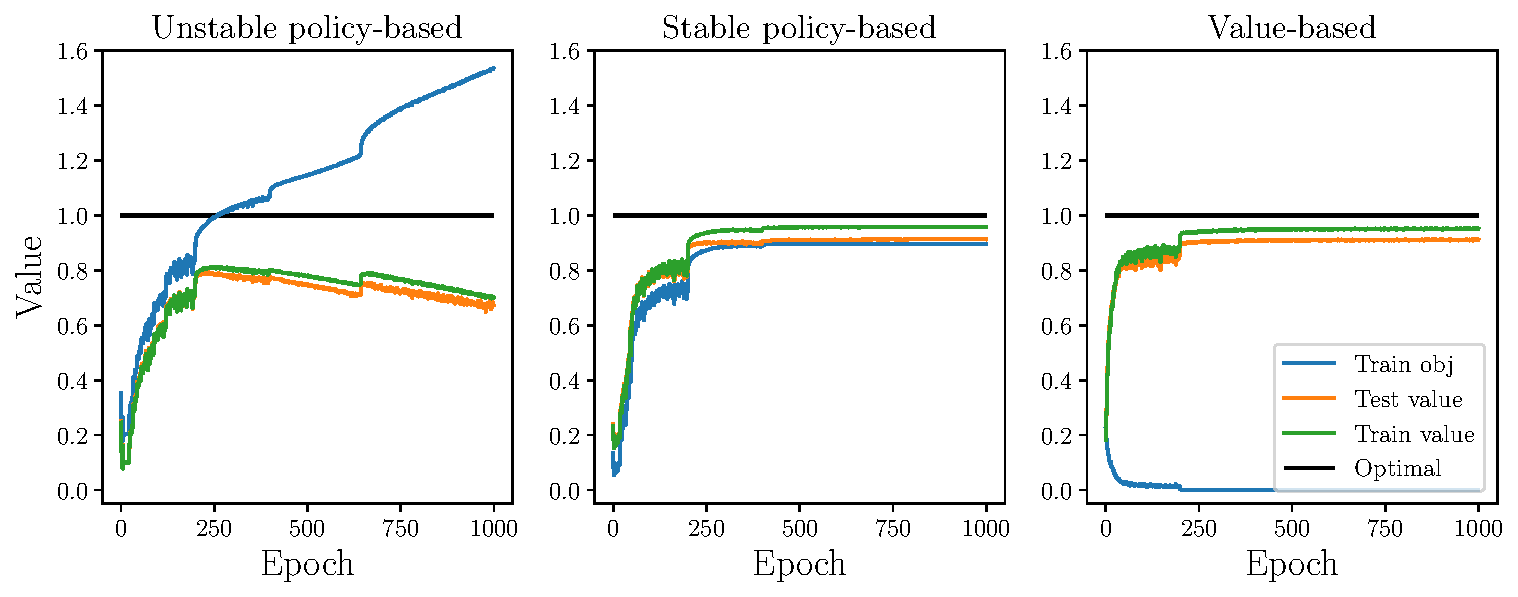
\includegraphics[width=0.7\textwidth]{figures/offline-bandits/cifar_learning_blbf.pdf}
    \caption{Learning curves on the hand-crafted action dataset.}
    \label{fig:cifar_learning_blbf}
\end{figure}


\begin{figure}[h]
    \centering
    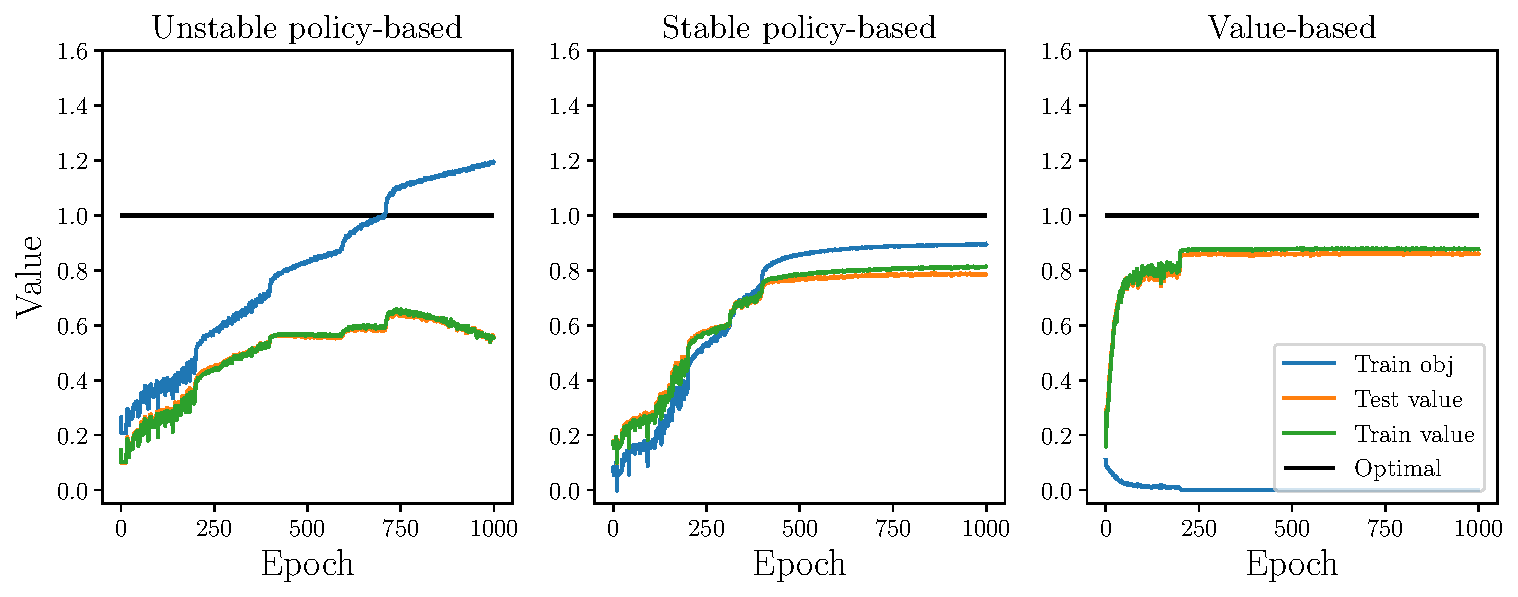
\includegraphics[width=0.7\textwidth]{figures/offline-bandits/cifar_learning_uniform_0.pdf}
    \caption{Learning curves on the uniform action dataset.}
    \label{fig:cifar_learning_uniform}
\end{figure}



\newappendix{Small model classes}\label{app:small}


In this section we state and prove theorems that bound each term of our regret decomposition for each algorithm we consider when we use finite model classes. Similar results can be shown for other classical notions of model class complexity. We include these results for completeness, but the main focus of our paper is the overparameterized regime where such bounds are vacuous.


\begin{theorem}[Policy-based learning with a small model class]\label{thm:pol-small}
Assume strict positivity and a finite policy class $ \Pi$. Let $ \varepsilon_\Pi = V(\pi^*) - \sup_{\pi \in \Pi} V(\pi)$. Denote $ \Delta_r = r_{max} - r_{min}$. Then we have that for any $ \delta > 0$ with probability $ 1- \delta$ each of the following holds:
\begin{align*}
    \text{Approximation Error} &= V(\pi^*) - \sup_{\pi\in \Pi}V(\pi) \leq \varepsilon_\Pi\\
    \text{Estimation Error}  &= \sup_{\pi\in \Pi}V(\pi) - V(\pi_F) \leq 2\Delta_r \sqrt{\frac{\log(2|\Pi|/\delta)}{2N}}\\
    \text{Bandit Error}  &= V(\pi_F) - V(\pi_B) \leq \frac{2\Delta_r}{\tau} \sqrt{\frac{\log(2|\Pi|/\delta)}{2N}}
\end{align*}
\end{theorem}
\begin{proof}
The bound on approximation error follows directly from the definition of $ \varepsilon_\Pi$. The bound on the estimation error follows from a standard application of a Hoeffding bound on the random variables $ X_i = \langle r_i, \pi(\cdot|x_i)\rangle
$ which are bounded by $ \Delta_r$ and a union bound over the policy class.

The bound on bandit error essentially follows Theorem 3.2 of \cite{strehl2010learning}, we include a proof for completeness:
\begin{align*}
    V(\pi_F) - V(\pi_B) &= V(\pi_F) - \hat V_B(\pi_B) + \hat V_B(\pi_B) - V(\pi_B) \\
    &\leq V(\pi_F) - \hat V_B(\pi_F) + \hat V_B(\pi_B) - V(\pi_B)\\
    &\leq 2 \sup_{\pi \in \Pi} |V(\pi) - \hat V_B(\pi)|\\
    &\leq \frac{2\Delta_r}{\tau} \sqrt{\frac{\log(2|\Pi|/\delta)}{2N}}
\end{align*}
The first inequality comes from the definition of $ \pi_B$. The second comes since both $ \pi_F, \pi_B \in \Pi$.
And the last inequality follows from an application of a Hoeffding bound on the random variables $ X_i = r_i(a_i)\frac{\pi(a_i|x_i)}{p_i}$ which are bounded by $ \frac{\Delta_r}{\tau}$ and a union bound over the policy class.
\end{proof}

\begin{theorem}[Value-based learning with a small model class]\label{thm:val-small}
Assume strict positivity and a finite function class $ \mathcal{Q}$ which induces a finite class of greedy policies $ \Pi_\mathcal{Q}$. Let $ \varepsilon_\mathcal{Q} = \inf_{\widehat Q\in \mathcal{Q}}\E_{x,a\sim \mathcal{D}, \beta}[(Q(x,a) - \widehat Q(x,a))^2]$. Denote $ \Delta_r = r_{max} - r_{min}$. Then we have that for any $ \delta > 0$ with probability $ 1- \delta$ each of the following holds:
\begin{align}
    \text{Approximation Error} &= V(\pi^*) - \sup_{\pi\in \Pi_{\mathcal{Q}}}V(\pi) \leq 2\sqrt{\varepsilon_{\mathcal{Q}}/ \tau}\\
    \text{Estimation Error}  &= \sup_{\pi\in \Pi_{\mathcal{Q}}}V(\pi) - V(\pi_F) \leq 2\Delta_r \sqrt{\frac{\log(|\mathcal{Q}|/\delta)}{2N}}\\
    \text{Bandit Error}  &= V(\pi_F) - V(\pi_{\widehat Q}) \leq \frac{10\Delta_r}{\sqrt{\tau}} \sqrt{\frac{\log(|\mathcal{Q}|/\delta)}{N}} + 6\sqrt{\Delta_r} \bigg(\frac{\log(|\mathcal{Q}|/\delta)}{\tau N} \varepsilon_{\mathcal{Q}}\bigg)^{1/4} + 2\sqrt{\varepsilon_{\mathcal{Q}}/ \tau}
\end{align}
\end{theorem}

\begin{proof}
To bound the approximation error, we can let $ \hat \pi $ be the greedy policy associated with a Q-function $ \widehat Q$ and apply Lemmas \ref{lem:mismatch} and \ref{lem:transfer}. This gives us
\begin{align}
        V(\pi^*) - \sup_{\hat \pi\in \Pi_{\mathcal{Q}}}V(\hat \pi) =  \inf_{\widehat Q\in \mathcal{Q}} [V(\pi^*) - V(\hat \pi)] \leq \inf_{\widehat Q\in \mathcal{Q}} \frac{2}{\sqrt{\tau}}\sqrt{\E_{x,a\sim \mathcal{D}, \beta}[(Q(x,a) - \widehat Q(x,a))^2]} = 2 \sqrt{\varepsilon_\mathcal{Q} / \tau}.
\end{align}
The bound on the estimation error follows the same as before from standard uniform convergence arguments.

The bound on the bandit error follows by again applying Lemmas \ref{lem:mismatch} and \ref{lem:transfer} and then making the concentration argument from Lemma 16 of \cite{chen2019information}. Explicitly, our Lemmas give us
\begin{align}
    V(\pi_F) - V(\pi_{\widehat Q}) \leq V(\pi^*) - V(\pi_{\widehat Q}) &\leq \frac{2}{\sqrt{\tau}} \sqrt{\E_{x,a\sim \mathcal{D}, \beta}[(Q(x,a) - \widehat Q(x,a))^2]}.
\end{align}
Then, to bound the squared error term, we can add and subtract:
\begin{align}
    \E_{x,a\sim \mathcal{D}, \beta}[(Q(x,a) - \widehat Q(x,a))^2] &= \E_{x,a\sim \mathcal{D}, \beta}[(Q(x,a) - \widehat Q(x,a))^2] - \inf_{\bar Q \in \mathcal{Q}}\E_{x,a\sim \mathcal{D}, \beta}[(Q(x,a) - \bar Q(x,a))^2] \\ &\qquad+ \inf_{\bar Q \in \mathcal{Q}}\E_{x,a\sim \mathcal{D}, \beta}[(Q(x,a) - \bar Q(x,a))^2]\\
    &\leq \E_{x,a\sim \mathcal{D}, \beta}[(Q(x,a) - \widehat Q(x,a))^2] - \inf_{\bar Q \in \mathcal{Q}}\E_{x,a\sim \mathcal{D}, \beta}[(Q(x,a) - \bar Q(x,a))^2] \\&\qquad+ \varepsilon_\mathcal{Q}.
\end{align}
Now we want to show that the difference in squared error terms concentrates for large $ N$. This is precisely what Lemma 16 from \cite{chen2019information} does using a one-sided Bernstein inequality. This gives us for any $ \delta > 0$ an upper bound with probability $ 1-\delta$ of
\begin{align}
    \frac{56\Delta_r^2 \log(|\mathcal{Q}|/\delta)}{3N} + \sqrt{\varepsilon_\mathcal{Q} \frac{32\Delta_r^2 \log(|\mathcal{Q}|/\delta)}{N}}
\end{align}
Plugging this in and simplifying the constants gives the result.
\end{proof}
\end{subappendices}




\printendnotes

\chapter{Offline RL Without Off-Policy Evaluation} \label{sec:offline-rl}
% \newcommand{\R}{\mathbb{R}}
\newcommand{\V}{\mathbb{V}}
% \newcommand{\E}{\mathop{\mathbb{E}}}
\newcommand{\Prob}{\mathbb{P}}



\section{Introduction}

% \begin{itemize}
%     \item Offline RL/ prior work

%     \item Summary of benchmark results (guidance)

%     \item What is holding multi-step back? evaluation error caused by distribution shift and iterative error exploitation

%     \item When can multi-step be more effective? Very broad coverage to estimate bad states. When behavior is good, one-step more effective.

%     \item Summarize contributions
% \end{itemize}

An important step towards effective real-world RL is to improve sample efficiency. One avenue towards this goal is offline RL (also known as batch RL) where we attempt to learn a new policy from data collected by some other behavior policy without interacting with the environment. Recent work in offline RL is well summarized by \citet{levine2020offline}.

In this paper, we challenge the dominant paradigm in the deep offline RL literature that primarily relies on actor-critic style algorithms that alternate between policy evaluation and policy improvement \citep{fujimoto2018off, fujimoto2019benchmarking, peng2019advantage, kumar2019stabilizing, kumar2020conservative, wang2020critic, wu2019behavior, kostrikov2021offline, jaques2019way, Siegel2020Keep, nachum2019algaedice}. All these algorithms rely heavily on off-policy evaluation to learn the critic. Instead, we find that a simple baseline which only performs one step of policy improvement using the behavior Q function often outperforms the more complicated iterative algorithms.
Explicitly, we find that our one-step algorithm beats prior results of iterative algorithms on most of the gym-mujoco \citep{brockman2016gym} and Adroit \citep{rajeswaran2017learning} tasks in the the D4RL benchmark suite \citep{fu2020d4rl}.

We then dive deeper to understand why such a simple baseline is effective. First, we examine what goes wrong for the iterative algorithms. When these algorithms struggle, it is often due to poor off-policy evaluation leading to inaccurate Q values. We attribute this to two causes: (1) distribution shift between the behavior policy and the policy to be evaluated, and (2) iterative error exploitation whereby policy optimization introduces bias and dynamic programming propagates this bias across the state space.
We show that empirically both issues exist in the benchmark tasks and that one way to avoid these issues is to simply avoid off-policy evaluation entirely.




Finally, we recognize that while the the one-step algorithm is a strong baseline, it is not always the best choice. In the final section we provide some guidance about when iterative algorithms can perform better than the simple one-step baseline. Namely, when the dataset is large and behavior policy has good coverage of the state-action space, then off-policy evaluation can succeed and iterative algorithms can be effective.
In contrast, if the behavior policy is already fairly good, but as a result does not have full coverage, then one-step algorithms are often preferable.

\begin{figure}[h]
    \centering
    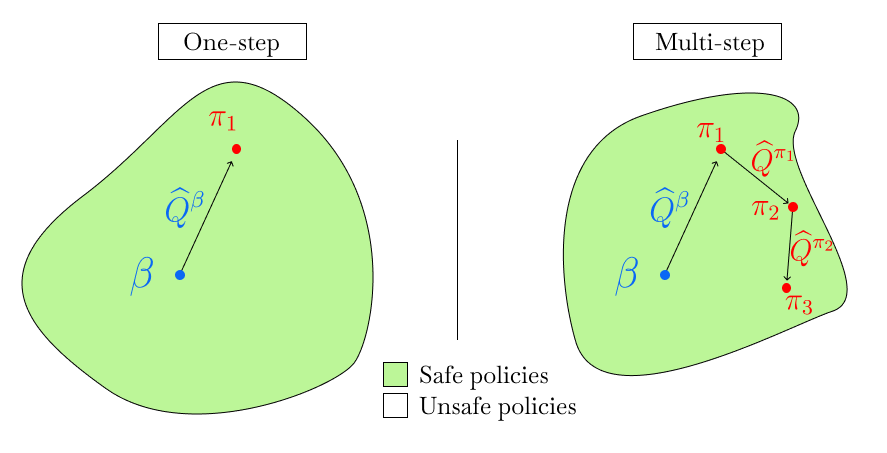
\includegraphics[width=0.6\textwidth]{figures/offline-rl/cartoon.png}
    \vspace{-0.2cm}
    \caption{A cartoon illustration of the difference between one-step and multi-step methods. All algorithms constrain themselves to a neighborhood of ``safe'' policies around $ \beta$. A one-step approach (left) only uses the \textcolor{blue}{on-policy} $ \widehat Q^\beta$, while a multi-step approach (right) repeatedly uses \textcolor{red}{off-policy} $\widehat Q^{\pi_i}$.
    % \joan{This is a nice illustration. I was wondering to what extent we could illustrate this neighborhood as a landscape (given by the objective function $J$) and show the two cartoon scenarios: (i) very smooth landscape, in which multi-step approaches would be worse off due to errors in estimating the gradient ($Q$), (ii) rugged landscape / valley, so that $\beta$ is in a basin that needs a non-linear path to keep descending. Also, we can illustrate what happens in off-policy updates, as the red arrows start drifting away from the true ones (not accessible)}
    }
    \label{fig:cartoon}
\end{figure}

Our main contributions are:
\begin{itemize}[leftmargin=*]
    \item A demonstration that a simple baseline of one step of policy improvement outperforms more complicated iterative algorithms on a broad set of offline RL problems.
    \item An examination of failure modes of off-policy evaluation in iterative offline RL algorithms.
    \item A description of when one-step algorithms are likely to outperform iterative approaches.
\end{itemize}



\vspace{0.2cm}
\section{Setting and notation}

We will consider an offline RL setup as follows. Let $ \mathcal{M} = \{\mathcal{S}, \mathcal{A}, \rho, P, R, \gamma \}$ be a discounted infinite-horizon  MDP.
In this work we focus on applications in continuous control, so we will generally assume that both $ \mathcal{S}$ and $ \mathcal{A}$ are continuous and bounded.
We consider the offline setting where rather than interacting with $\mathcal{M}$, we only have access to a dataset $ D_N$ of $ N $ tuples of $ (s_i, a_i, r_i)$ collected by some behavior policy $ \beta$ with initial state distribution $ \rho$.
Let $ r(s,a) = \E_{r|s,a}[r]$ be the expected reward.
Define the state-action value function for any policy $ \pi$ by $ Q^\pi(s,a) := \E_{P, \pi | s_0 = s,\ a_0 = a}[\sum_{t=0}^\infty \gamma^t r(s_t, a_t)]$.
The objective is to maximize the expected return $ J $ of the learned policy:
\begin{align}
    J(\pi) := \E_{\rho, P, \pi}\left[ \sum_{t=0}^\infty \gamma^t r(s_t, a_t) \right] = \E_{\substack{s\sim \rho\\ a \sim \pi|s}}[Q^\pi(s,a)]. % \frac{1}{1-\gamma} \E_{s\sim d^\pi_\rho} \E_{a\sim \pi|s}[r(s,a)]
\end{align}
Following \citet{fu2020d4rl} and others in this line of work, we allow access to the environment to tune a small (< 10) set of hyperparameters.
See \citet{paine2020hyperparameter} for a discussion of the active area of research on hyperparameter tuning for offline RL.
We also discuss this further in Appendix \ref{sec:app_exp_setup}.


\section{Related work}

Most prior work on deep offline RL consists of iterative actor-critic algorithms. The primary innovation of each paper is to propose a different mechanism to ensure that he learned policy does not stray too far from the data generated by the behavior policy. Broadly, we group these methods into three camps: policy constraints/regularization, modified of imitation learning, and Q regularization:

\begin{enumerate}[leftmargin=*]
\item The majority of prior work acts directly on the policy.
Some authors have proposed explicit constraints on the learned policy to only select actions where $ (s,a)$ has sufficient support under the data generating distribution \citep{fujimoto2018off, fujimoto2019benchmarking, laroche2019safe}.
Another proposal is to regularize the learned policy towards the behavior policy \citep{wu2019behavior} usually either with a KL divergence \citep{jaques2019way} or MMD \citep{kumar2019stabilizing}. This is a very straighforward way to stay close to the behavior with a hyperparameter that determines just how close. All of these algorithms are iterative and rely on off-policy evaluation.

\item \citep{Siegel2020Keep, wang2020critic, chen2020bail} all use algorithms that filter out datapoints with low Q values and then perform imitation learning.
\citep{wang2018exponentially, peng2019advantage} use a weighted imitation learning algorithm where the weights are determined by exponentiated Q values.
These algorithms are iterative.
\item Another way to prevent the learned policy from choosing unknown actions is to incorporate some form of regularization to encourage staying near the behavior and being pessimistic about unknown state, action pairs \citep{wu2019behavior, nachum2019algaedice, kumar2020conservative, kostrikov2021offline}.
However, properly being able to quantify uncertainty about unknown states is notoriously difficult when dealing with neural network value functions \citep{buckman2020importance}.
Again all of these algorithms are iterative.
\end{enumerate}


Some recent work has also noted that optimizing policies based on the behavior value function can perform surprisingly well \citep{gulcehre2020rl, goo2020you}. However, these papers propose complicated variants of the one-step approach involving ensembles, non-standard regularizers and paraterizations or ensembles and distributional Q functions. In contrast, we implement the simplest possible one-step algorithms without any modifications to the network architecture or standard regularizers/constraints.
Moreover, we focus on providing an analysis of when and why this simple baseline works.

There are also important connections between the one-step algorithm and the literature on conservative policy improvement \citep{kakade2002approximately, schulman2015trust, achiam2017constrained}, which we discuss in more detail in Appendix \ref{sec:app_improvement}.


\section{Defining the algorithms}

In this section we provide a unified algorithmic template for offline RL algorithms as offline approximate modified policy iteration. We show how this template captures our one-step algorithm as well as a multi-step policy iteration algorithm and an iterative actor-critic algorithm.
Then any choice of policy evaluation and policy improvement operators defines one-step, multi-step, and iterative algorithms.

%Full details about our implementation can be found in Appendix \warn{write up implementation}.

\subsection{Algorithmic template}

We consider a generic offline approximate modified policy iteration (OAMPI) scheme, shown in Algorithm \ref{alg:oapi}. Essentially the algorithm alternates between two steps. First, there is a policy evaluation step where we estimate the Q function of the current policy $ \pi_{k-1}$ by $ \widehat Q^{\pi_{k-1}}$ using only the dataset $ D_N$. Implementations also often use the prior Q estimate $ \widehat Q^{\pi_{k-2}}$ to warm-start the approximation process. Second, there is a policy improvement step. This step takes in the estimated Q function $ \widehat Q^{\pi_{k-1}}$, the estimated behavior $ \hat \beta$, and the dataset $ D_N$ and produces a new policy $ \pi_k$. Again an algorithm may use $ \pi_{k-1}$ to warm-start the optimization. Moreover, we expect this improvement step to be regularized or constrained to ensure that $ \pi_k$ remains in the support of $ \beta$ and $ D_N$. Choices for this regularization/constraint are discussed below. Now we discuss a few ways to instantiate the template.

\begin{figure*}[h]
\vspace{-0.5cm}
\begin{algorithm}[H]
    \caption{OAMPI} \label{alg:oapi}
    \begin{algorithmic}[1]
             \Require{$ K$, dataset $ D_N$,  estimated behavior $ \hat \beta$}
             \State Set $\pi_0 = \hat \beta$. Initialize $ \widehat Q^{\pi_{-1}}$ randomly.
             \For{k = 1, \dots, K}
                \State Policy evaluation: $ \widehat Q^{\pi_{k-1}} = \mathcal{Q}(\pi_{k-1}, D_N, \widehat Q^{\pi_{k-2}})$
                \State Policy improvement: $ \pi_{k} = \mathcal{I}(\widehat Q^{\pi_{k-1}}, \hat \beta, D_N, \pi_{k-1})$
             \EndFor
        \end{algorithmic}
    \end{algorithm}
\end{figure*}



\paragraph{One-step.}
The simplest algorithm sets the number of iterations $ K = 1$. We train the policy evaluation to estimate $ Q^\beta$, and then use one of the policy improvement operators discussed below to find the resulting $ \pi_1$.


\paragraph{Multi-step.}
The multi-step algorithm now sets $ K >1$. The evaluation operator must evaluate off-policy since $ D_N$ is collected by $ \beta$, but evaluation steps for $ K \geq 2$ require evaluating policies $ \pi_{k-1}\neq \beta$. Each iteration is trained to convergence in both the estimation and improvement steps.

\paragraph{Iterative actor-critic.}

An actor critic approach looks somewhat like multistep policy iteration, but does not attempt to train to convergence at each iteration. Instead, each iteration consists of one gradient step to update the Q estimate and one gradient step to improve the policy. Since all of the evaluation and improvement operators that we consider are gradient-based, this algorithm can adapt the same evaluation and improvement operators used by the multi-step algorithm. Most algorithms from the literature fall into this category \citep{fujimoto2018off, kumar2019stabilizing, kumar2020conservative, wu2019behavior,  wang2020critic, Siegel2020Keep}.


\subsection{Policy evaluation operators}

Following prior work on continuous state and action problems, we always evaluate by simple fitted Q evaluation \citep{fujimoto2018off, kumar2019stabilizing, Siegel2020Keep, wang2020critic, paine2020hyperparameter, wang2021instabilities}.
Explicitly the evaluation step for the one-step or multi-step algorithms looks like
\begin{align}
     \mathcal{Q}(\pi_{k-1}, D_N, \widehat Q^{\pi_{k-2}}) = \arg\min_Q \sum_{i=1}^N \left(r(s_i,a_i) + \gamma \E_{a'\sim \pi_{k-1}|s_i'}Q(s_i', a') - Q(s_i, a_i) \right)^2,
\end{align}
where the right hand side may depend on $\widehat Q^{\pi_{k-2}}$ to warm-start optimization.
In practice this is optimized by stochastic gradient descent with the use of a target network \citep{mnih2015human}.
For the iterative algorithm the $ \arg\min$ is replaced by a single stochastic gradient step.
We estimate the expectation over next state by a single sample from $ \pi_{k-1}$ (or from the dataset in the case when $ \pi_{k-1} = \hat \beta$). See \cite{voloshin2019empirical, wang2021instabilities} for more comprehensive examinations of this evaluation step.



\subsection{Policy improvement operators}

To instantiate the template, we also need to choose a specific policy improvement operator $ \mathcal{I}$. We consider the following improvement operators selected from those discussed in the related work section. Each operator has a hyperparameter controlling deviation from the behavior policy.

\paragraph{Behavior cloning.} The simplest baseline worth including is to just return $ \hat \beta$ as the new policy $ \pi$. Any policy improvement operator ought to perform at least as well as this baseline.


% \paragraph{Greedy.} The naive policy improvement operator just acts greedily with respect to $ \widehat Q^\beta$ so that $\hat \pi(a|s) = \one[a = \arg\max_{a'} \widehat Q^\beta(s, a')]$.
% Calculating this arg max may not feasible in a continuous action space, so we can instead amortize the computation by learning a neural network policy to maximize the estimated Q values such that
% \begin{align}
%     \pi_k = \mathcal{I}(\widehat Q, \hat \beta, D_N, \pi_{k-1}) =  \arg\max_{\pi} \sum_i \E_{a\sim \pi|s_i} [\widehat Q (s_i, a)]
% \end{align}
% where the optimization can be performed using stochastic optimization via the reparameterization trick. Specifically, at each iteration we (1) sample a minibatch of datapoints, (2) sample one reparameterized action for each state in the minibatch, and then (3) backpropogate to get a stochastic gradient estimate.


\paragraph{Constrained policy updates.}
Algorithms like BCQ \citep{fujimoto2018off} and SPIBB \citep{laroche2019safe} constrain the policy updates to be within the support of the data/behavior.
% The SPIBB algorithm requires uncertainty estimates that are difficult to quantify in continuous state and action spaces, and both of these algorithms are somewhat complicated.
In favor of simplicity, we implement a simplified version of the BCQ algorithm that removes the policy correction network which we call Easy BCQ.
We define a new policy $ \hat \pi^M_{k}$ by drawing $ M $ samples from $ \hat \beta$ and then executing the one with the highest value according to $ \widehat Q^\beta$. Explicitly:
\begin{align}
    \hat \pi^M_{k}(a|s) = \one[a = \arg\max_{a_j} \{\widehat Q^{\pi_{k-1}}(s, a_j): a_j \sim \pi_{k-1}(\cdot|s),\ 1 \leq j \leq M\}].
\end{align}

% Note, we can think about this policy in terms of pushforward distributions where we are taking an $ n$th order statistic of $ M $ samples from $ \widehat Q_\sharp^\beta (s, \hat \beta)$. If we let $ F$ be the CDF of $ \widehat Q_\sharp^\beta (s, \hat \beta)$ and $ F_M$ be the CDF of $ \widehat Q_\sharp^\beta (s, \hat \pi_M)$, it is straightforward to see that
% \begin{align}
%     F_M(v) = F(v)^M.
% \end{align}
% Thus, we know that we are moving mass in a strictly increasing way, and can come up with a policy improvement guarantee similar to the one we have for QFIL, but in terms of the difference between $ F(v) $ and $ F(v)^M$.

% This sort of analysis is novel since prior work on BCQ \citep{fujimoto2018addressing} proposes a more complicated algorithm and only provides a tabular analysis.



\paragraph{Regularized policy updates.}
Another common idea proposed in the literature is to regularize towards the behavior policy \citep{wu2019behavior, jaques2019way, kumar2019stabilizing, ma2019imitation}. For a general divergence $ D$ we can define an algorithm that maximizes a regularized objective:
\begin{align}
    \hat \pi^\alpha_k = \arg\max_\pi \sum_{i}  \E_{a\sim \pi|s}[\widehat Q^{\pi_{k-1}}(s_i, a)] - \alpha D(\hat \beta(\cdot|s_i), \pi(\cdot|s_i))
\end{align}

A comprehensive review of different variants of this method can be found in \cite{wu2019behavior} which does not find dramatic differences across regularization techniques.
In practice, we will use reverse KL divergence,  i.e. $ KL( \pi(\cdot|s_i) \| \hat \beta(\cdot|s_i))$.
%For the forward KL, i.e. $ KL(\beta(\cdot|s_i) \| \pi(\cdot|s_i))$, we can simply use the sampled action $ a_i$ from the dataset to estimate the divergence.
To compute the reverse KL, we draw samples from $ \pi(\cdot |s_i)$ and use the density estimate $ \hat \beta$ to compute the divergence. Intuitively, this regularization forces $ \pi$ to remain within the support of $ \beta$ rather than incentivizing $ \pi$ to cover beta.


\paragraph{Variants of imitation learning.}
Another idea, proposed by \citep{wang2018exponentially, Siegel2020Keep, wang2020critic, chen2020bail} is to modify an imitation learning algorithm either by filtering or weighting the observed actions so as to get a policy improvement. The weighted version that we implement uses exponentiated advantage estimates to weight the observed actions:
\begin{align}
    \hat \pi^\tau_k = \arg\max_\pi \sum_{i}  \exp(\tau (\widehat Q^{\pi_{k-1}}(s_i, a_i) - \widehat V(s_i))) \log \pi(a_i|s_i).
\end{align}
%This can also be derived as a variational implementation of the reverse-KL regularized update, as is done in \cite{wang2018exponentially}.

% \begin{align}
%     \hat \pi_b (a|s) = \arg\max_\pi \sum_{i}  \1[\widehat Q^\beta(s_i, a_i) \geq b(s_i)] \log \pi(a_i|s_i)
% \end{align}





\section{Benchmark Results}\label{sec:bench}

Our main empirical finding is that one step of policy improvement is sufficient to beat state of the art results on much of the D4RL benchmark suite \cite{fu2020d4rl}.
This is striking since prior work focuses on iteratively estimating the Q function of the current policy iterate, but we only use one-step derived from $ \widehat Q^\beta$. Results are shown in Table~\ref{tab:d4rl}. Full experimental details are in Appendix \ref{sec:app_exp_setup}.

\begin{table}[h]
    \centering
    \caption{Results of one-step algorithms on the D4RL benchmark. The first column gives the best results across several iterative algorithms considered in \cite{fu2020d4rl}. We run 3 seeds and each algorithm is tuned over 6 values of their respective hyperparameter. We report the mean and standard deviation over seeds on 100 evaluation episodes per seed. We \textbf{bold} the best result on each dataset and \textcolor{blue}{blue} any result where a one-step algorithm beat the best reported iterative result from \cite{fu2020d4rl}. We use m for medium, m-e for medium-expert, m-re for medium-replay, r for random, and c for cloned.}
    \begin{small}
    \begin{tabular}{lccccc}
        \toprule & Iterative & \multicolumn{4}{c}{One-step}\\
        \cmidrule(lr){2-2} \cmidrule(lr){3-6}
         & \cite{fu2020d4rl} & BC & Easy BCQ  & Rev. KL Reg & Exp. Weight \\
        \midrule
        halfcheetah-m & 46.3 &
                        41.9  $\pm$  0.1 &
                        \textcolor{blue}{52.6  $\pm$  0.2}  &
                        \textcolor{blue}{\textbf{55.2  $\pm$  0.4 }} &
                        \textcolor{blue}{48.4  $\pm$  0.1} \\
        walker2d-m & 81.1 &
                        68.6  $\pm$  6.3 &
                        \textcolor{blue}{\textbf{87.2  $\pm$  1.3}} &
                        \textcolor{blue}{85.9  $\pm$  1.4} &
                        \textcolor{blue}{81.8  $\pm$  2.2}  \\
        hopper-m & 58.8 &
                        49.9  $\pm$  3.1 &
                        \textcolor{blue}{74.5  $\pm$  6.2}&
                        \textcolor{blue}{\textbf{83.7  $\pm$  4.5}} &
                        \textcolor{blue}{59.6  $\pm$  2.5}\\
        \midrule
        halfcheetah-m-e & 64.7 &
                        61.1  $\pm$  2.7 &
                        \textcolor{blue}{78.2  $\pm$  1.6}  &
                        \textcolor{blue}{\textbf{93.8  $\pm$  0.5}} &
                        \textcolor{blue}{93.4  $\pm$  1.6} \\
        walker2d-m-e & 111.0 &
                        78.5  $\pm$  22.4 &
                        \textcolor{blue}{112.2  $\pm$  0.3}   &
                        \textcolor{blue}{111.2  $\pm$  0.2}  &
                        \textcolor{blue}{\textbf{113.0  $\pm$  0.4}}  \\
        hopper-m-e & \textbf{111.9} &
                        49.1  $\pm$  4.3 &
                        85.1  $\pm$  2.2 &
                        98.7  $\pm$  7.5 &
                        103.3  $\pm$  9.1 \\
        \midrule
        halfcheetah-m-re & \textbf{47.7} &
                         34.6  $\pm$  0.9 &
                         38.3  $\pm$  0.3  &
                        41.9  $\pm$  0.5 &
                         38.1  $\pm$  1.3 \\
        walker2d-m-re & 26.7 &
                        26.6  $\pm$  3.4  &
                         \textcolor{blue}{69.1  $\pm$  4.2} &
                        \textcolor{blue}{\textbf{74.9  $\pm$  6.6}} &
                         \textcolor{blue}{49.5  $\pm$  12.0}  \\
        hopper-m-re & 48.6 &
                       23.1  $\pm$  2.7 &
                        \textcolor{blue}{78.4  $\pm$  7.2} &
                        \textcolor{blue}{92.3  $\pm$  1.1} &
                        \textcolor{blue}{\textbf{97.5  $\pm$  0.7}}\\
        \midrule
        halfcheetah-r & \textbf{35.4} &
                        2.2  $\pm$  0.0 &
                        5.4  $\pm$  0.3 &
                        8.8  $\pm$  3.8   &
                        3.2  $\pm$  0.1 \\
        walker2d-r & \textbf{7.3} &
                        0.9  $\pm$  0.1 &
                        3.7  $\pm$  0.1  &
                        6.2  $\pm$  0.7 &
                        5.6  $\pm$  0.8 \\
        hopper-r & \textbf{12.2} &
                        2.0  $\pm$  0.1 &
                        6.6  $\pm$  0.1 &
                        7.9  $\pm$  0.7 &
                        7.5  $\pm$  0.4  \\
        \midrule
        pen-c & 56.9 &
                    46.9  $\pm$  11.0 &
                    \textcolor{blue}{\textbf{65.9  $\pm$  3.6}} &
                    \textcolor{blue}{57.4  $\pm$  3.5} &
                    \textcolor{blue}{60.0  $\pm$  4.1} \\
        hammer-c & 2.1 &
                    0.4  $\pm$  0.1  &
                    \textcolor{blue}{\textbf{2.9  $\pm$  0.5 }} &
                    0.2  $\pm$  0.1 &
                    2.1  $\pm$  0.7  \\
        relocate-c & -0.1 &
                    -0.1  $\pm$  0.0 &
                    \textcolor{blue}{\textbf{0.3  $\pm$  0.2}} &
                    \textcolor{blue}{0.2  $\pm$  0.1} &
                    \textcolor{blue}{0.2  $\pm$  0.1}   \\
         door-c & 0.4 &
                    0.0  $\pm$  0.1 &
                    \textcolor{blue}{\textbf{0.6  $\pm$  0.6}} &
                    0.2  $\pm$  0.7 &
                    0.2  $\pm$  0.3 \\
        \bottomrule
    \end{tabular}
    \end{small}
    \label{tab:d4rl}
\end{table}

% Goo:
% m: 35.6,  68.6, 76.4
% m-e: 16.6,  92.7, 106.4,
% m-re: 34.4,  41.5, 94.8
% r: 7.2, 8.1, 9.8
% c: 61.2, 0.4, -0.2, 1.1



As we can see in the table, all of the one-step algorithms usually outperform the best iterative algorithms tested by \citet{fu2020d4rl}.
The one notable exception is the case of random data (especially on halfcheetah), where iterative algorithms have a clear advantage. We will discuss potential causes of this further in Section \ref{sec:when}.

To give a more direct comparison that controls for any potential implementation details, we use our implementation of reverse KL regularization to create multi-step and iterative algorithms. We are not using algorithmic modifications like Q ensembles, regularized Q values, or early stopping that have been used in prior work. But, our iterative algorithm recovers similar performance to prior regularized actor-critic approaches. These results are shown in Table~\ref{tab:multi}.

\begin{table}[h]
\vspace{-0.5 cm}
    \centering
    \caption{Results of reverse KL regularization on the D4RL benchmark across one-step, multi-step, and iterative algorithms. Again we run 3 seeds and 6 hyperparameters and report the mean and standard deviation across seeds using 100 evaluation episodes.}
    \begin{small}
    \begin{tabular}{lccc}
        \toprule
         & One-step & Multi-step & Iterative \\
        \midrule
        halfcheetah-m &
                        55.2  $\pm$  0.4  &
                        \textbf{59.3  $\pm$  0.7} &
                        51.2  $\pm$  0.2\\
        walker2d-m &
                        \textbf{85.9  $\pm$  1.4} &
                        74.5  $\pm$  2.8    &
                        74.8  $\pm$  0.7  \\
        hopper-m &
                        \textbf{83.7  $\pm$  4.5} &
                        54.8  $\pm$  4.3  &
                        54.7  $\pm$  1.9\\
        \midrule
        halfcheetah-m-e &
                        93.8  $\pm$  0.5 &
                        \textbf{94.2  $\pm$  0.5} &
                        93.7  $\pm$  0.6 \\
        walker2d-m-e &
                        \textbf{111.2  $\pm$  0.2} &
                        109.8  $\pm$  0.3  &
                        108.7  $\pm$  0.6 \\
        hopper-m-e &
                        \textbf{98.7  $\pm$  7.5} &
                        90.6  $\pm$  18.8 &
                        94.5  $\pm$  11.9\\
        \midrule
        halfcheetah-r &
                        8.8  $\pm$  3.8  &
                        18.3  $\pm$  6.5 &
                        \textbf{21.2  $\pm$  5.2}\\
        walker2d-r &
                        \textbf{6.2  $\pm$  0.7} &
                        5.4  $\pm$  0.2 &
                        5.4  $\pm$  0.4\\
        hopper-r &
                        7.9  $\pm$  0.7 &
                        \textbf{21.9  $\pm$  8.9} &
                        9.7  $\pm$  0.4\\
        \bottomrule
    \end{tabular}
    \end{small}
    \label{tab:multi}
\end{table}

Put together, these results immediately suggest some guidance to the practitioner: it is worthwhile to run the one-step algorithm as a baseline before trying something more elaborate. The one-step algorithm is substantially simpler than prior work, but usually achieves better performance.



% \subsection{Benchmarking QFIL}

% \begin{figure}[h]
%     \centering
%     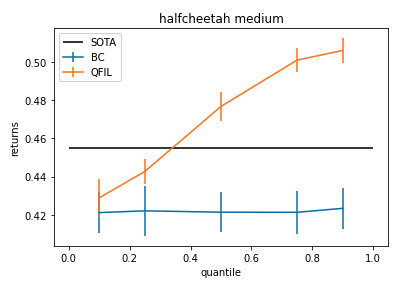
\includegraphics[width=0.3\textwidth]{figures/offline-rl/benchmark/hc-m.png}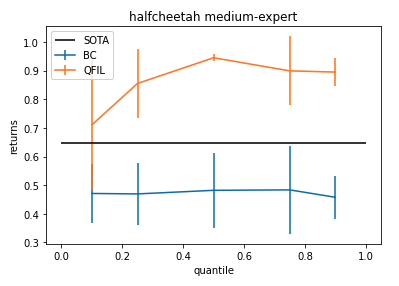
\includegraphics[width=0.3\textwidth]{figures/offline-rl/benchmark/hc-me.png}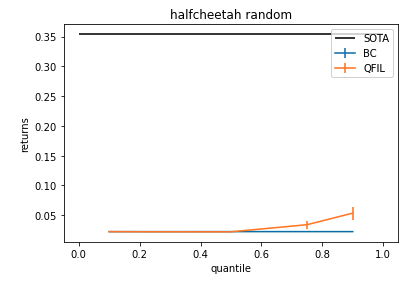
\includegraphics[width=0.3\textwidth]{figures/offline-rl/benchmark/hc-r.png}\\
%     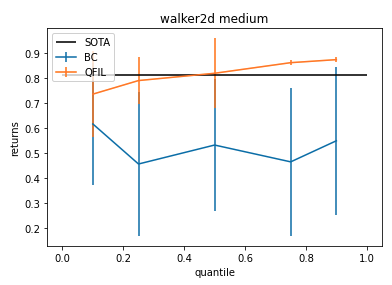
\includegraphics[width=0.3\textwidth]{figures/offline-rl/benchmark/w-m.png}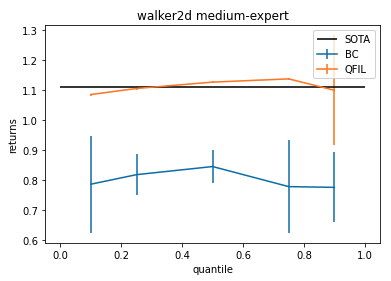
\includegraphics[width=0.3\textwidth]{figures/offline-rl/benchmark/w-me.png}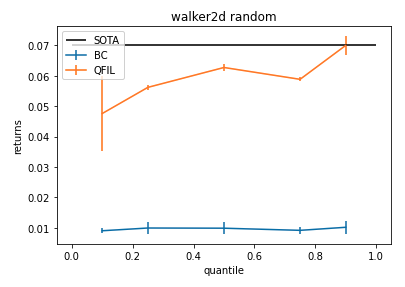
\includegraphics[width=0.3\textwidth]{figures/offline-rl/benchmark/w-r.png}\\
%     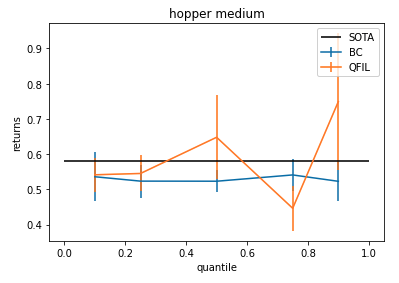
\includegraphics[width=0.3\textwidth]{figures/offline-rl/benchmark/h-m.png}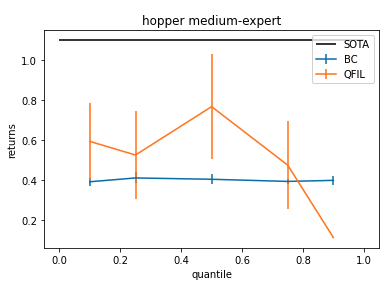
\includegraphics[width=0.3\textwidth]{figures/offline-rl/benchmark/h-me.png}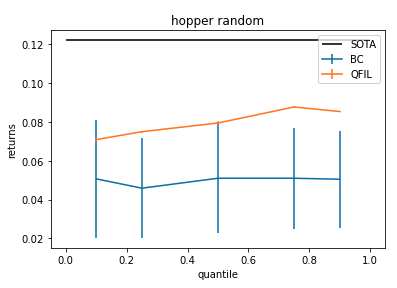
\includegraphics[width=0.3\textwidth]{figures/offline-rl/benchmark/h-r.png}
%     \caption{Results on the D4RL benchmark, with state of the art (SOTA) taken from \cite{fu2020d4rl}. \qfil\ beats the state of the art on 6 out of 9 datasets shown in the figure and always makes a substantial improvement over behavior cloning (BC).}
%     \label{fig:benchmark}
% \end{figure}











\section{What goes wrong for iterative algorithms?}\label{sec:why}


% \subsection{Policy improvement perspective}

% We can modify the performance difference lemma to measure the difference between two policies $ \pi_1, \pi_2$ using the state distribution derived from the behavior $ \beta$.

% \begin{lemma}[Approximate three-way performance difference]
% For any three policies $ \pi_2, \pi_1$ and $ \beta$,
% \begin{align}
%     (1-\gamma) (J(\pi_2) &- J(\pi_1)) = \underbrace{\E_{s\sim d_\beta}[\widehat Q^{\pi_1}(s,\pi_2) - \widehat Q^{\pi_1}(s,{\pi_1})]}_{Estimated\ improvement} \\ &- \underbrace{\E_{s\sim d_\beta}\left[(\widehat Q^{\pi_1}(s,\pi_2) - Q^{\pi_1}(s, \pi_2)) + (Q^{\pi_1}(s,{\pi_1}) - \widehat Q^{\pi_1}(s, {\pi_1})) \right]}_{Evaluation\ error}\\
%     &- \underbrace{\E_{\substack{s\sim d_\beta \\ s' \sim d_{\pi_2}}}\left[(Q^{\pi_1}(s, \pi_2) - Q^{\pi_1}(s', \pi_2) ) + (Q^{\pi_1}(s', \pi_1) - Q^{\pi_1}(s, \pi_1)) \right]}_{State\ distribution\ mismatch}
% \end{align}
% \end{lemma}

The benchmark experiments show that one step of policy improvement often beats iterative and multi-step algorithms. In this section we dive deeper to understand why this happens. First, by examining the learning curves of each of the algorithms we note that iterative algorithms require stronger regularization to avoid instability. Then we identify two causes of this instability: \emph{distribution shift} and \emph{iterative error exploitation}.

Distribution shift causes evaluation error by reducing the effective sample size in the fixed dataset for evaluating the current policy and has been extensively considered in prior work as discussed below. Iterative error exploitation occurs when we repeatedly optimize policies against our Q estimates and exploit their errors. This introduces a bias towards overestimation at each step (much like the training error in supervised learning is biased to be lower than the test error). Moreover, by iteratively re-using the data and using prior Q estimates to warmstart training at each step, the errors from one step are amplified at the next. This type of error is particular to multi-step and iterative algorithms.

\subsection{Learning curves and hyperparameter sensitivity}

To begin to understand why iterative and multi-step algorithms can fail it is instructive to look at the learning curves. As shown in Figure \ref{fig:learning_curves}, we often observe that the iterative algorithm will begin to learn and then crash. Regularization can help to prevent this crash since strong enough regularization towards the behavior policy ensures that the evaluation is nearly on-policy.

\begin{figure}[h]
    \centering
    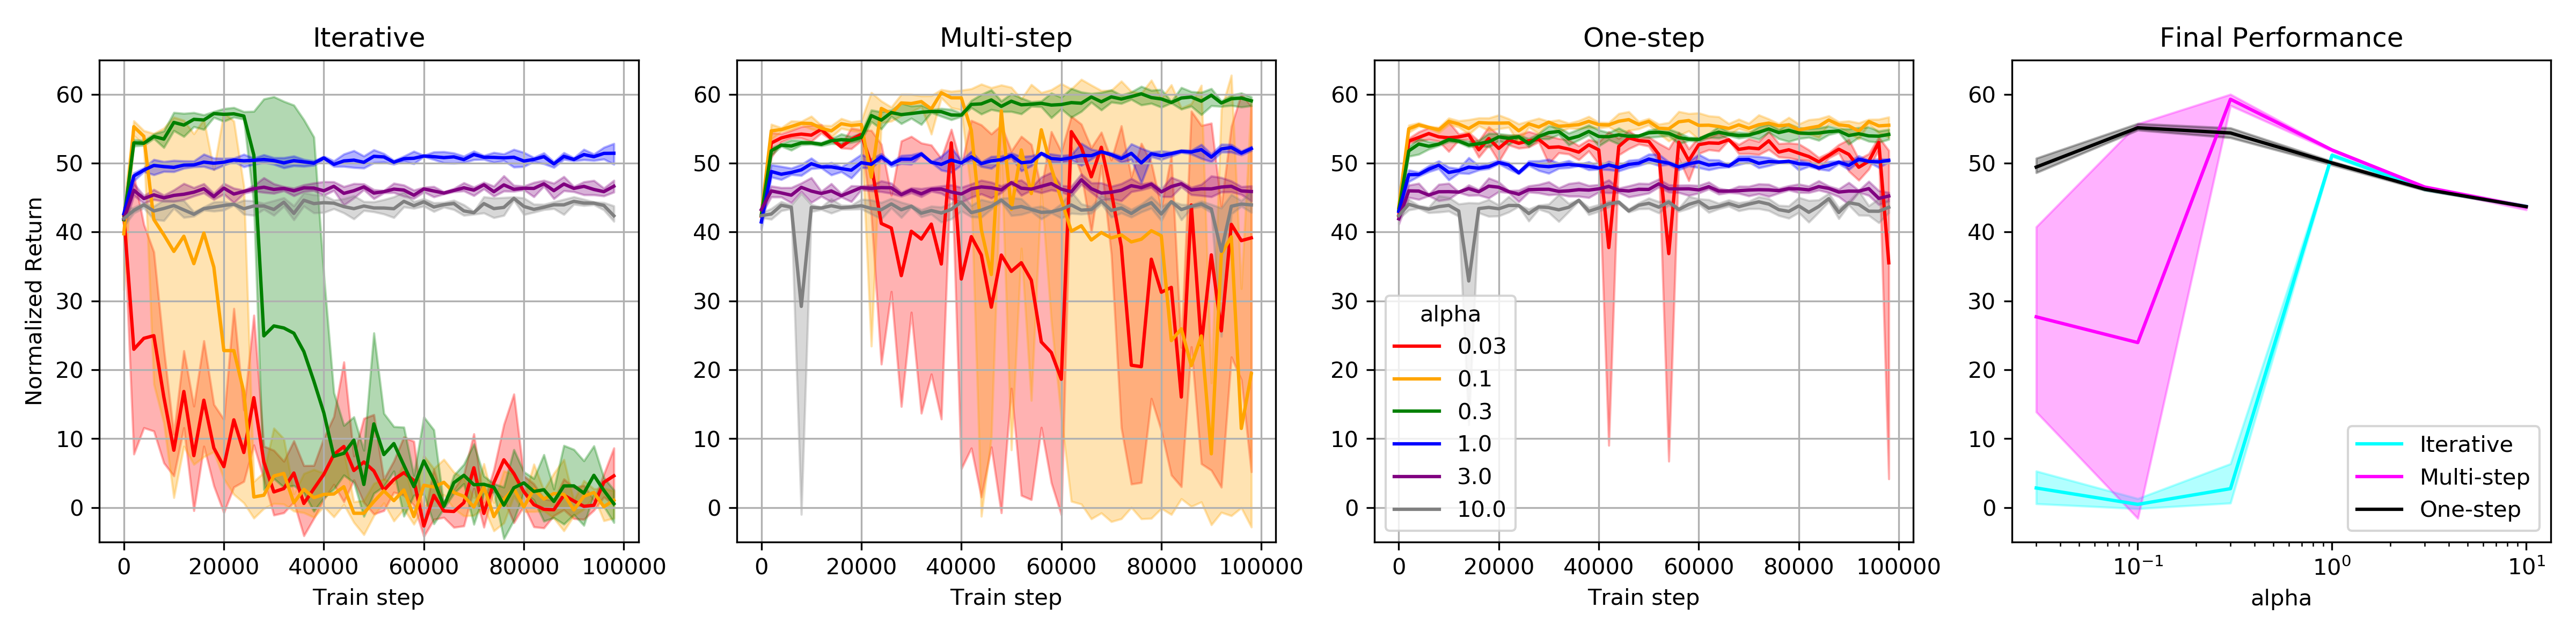
\includegraphics[width=\textwidth]{figures/offline-rl/learning curves/learning_curves.png}
    \caption{Learning curves and final performance on halfcheetah-medium across different algorithms and regularization hyperparameters. Error bars show min and max over 3 seeds. Similar figures for other datasets from D4RL can be found in Appendix~\ref{sec:app_extra_exp}.}
    \label{fig:learning_curves}
\end{figure}

In contrast, the one-step algorithm is more robust to the regularization hyperparameter. The rightmost panel of the figure shows this clearly. While iterative and multi-step algorithms can have their performance degrade very rapidly with the wrong setting of the hyperparameter, the one-step approach is more stable.
Moreover, we usually find that the optimal setting of the regularization hyperparameter is lower for the one-step algorithm than the iterative or multi-step approaches.







\subsection{Distribution shift}

Any algorithm that relies on off-policy evaluation will struggle with distribution shift in the evaluation step. Trying to evaluate a policy that is substantially different from the behavior reduces the effective sample size and increases the variance of the estimates. Explicitly, by distribution shift we mean the shift between the behavior distribution (the distribution over state-action pairs in the dataset) and the evaluation distribution (the distribution that would be induced by the policy $ \pi$ we want to evaluate).

\paragraph{Prior work.} There is a substantial body of prior theoretical work that suggests that off-policy evaluation can be difficult and this difficulty scales with some measure of distribution shift.
%\cite{jiang2016doubly} give an exponential (in horizon) lower bound on sample complexity in the tabular setting for any unbiased estimator from the Cramer-Rao lower bound.
\citet{wang2020statistical, Amortila2020AVO, zanette2021exponential} give exponential (in horizon) lower bounds on sample complexity in the linear setting even with good feature representations that can represent the desired Q function and assuming good data coverage.
Upper bounds generally require very strong assumptions on both the representation and limits on the distribution shift \citep{wang2021instabilities, duan2020minimax, chen2019information}. Moreover, the assumed bounds on distribution shift can be exponential in horizon in the worst case.
% The literature on policy improvement also suggests limiting distribution shift \citep{kakade2002approximately, schulman2015trust, achiam2017constrained}. We discuss how the guarantees from this literature apply directly to the one-step but not multi-step algorithms in more detail in Appendix \ref{sec:app_improvement}. \warn{TODO: link this in better}
On the empirical side, \citet{wang2021instabilities} demonstrates issues with distribution shift when learning from pre-trained features and provides a nice discussion of why distribution shift causes error amplification. \citet{fujimoto2018off} raises a similar issue under the name ``extrapolation error''. Regularization and constraints are meant to reduce issues stemming from distribution shift, but also reduce the potential for improvement over the behavior.


\paragraph{Empirical evidence.} Both the multi-step and iterative algorithms in our experiments rely on off-policy evaluation as a key subroutine. We examine how easy it is to evaluate the policies encountered along the learning trajectory. To control for issues of iterative error exploitation (discussed in the next subsection), we train Q estimators from scratch on a heldout evaluation dataset sampled from the behavior policy. We then evaluate these trained Q function on rollouts from 1000 datapoints sampled from the replay buffer. Results are shown in Figure~\ref{fig:mse}.


The results show a correlation betweed KL and MSE. Moreover, we see that the MSE generally increases over training. One way to mitigate this, as seen in the figure, is to use a large value of $ \alpha$. We just cannot take a very large step before running into problems with distribution shift. But, when we take such a small step, the information from the on-policy $ \widehat Q^\beta$ is about as useful as the newly estimated $ \widehat Q^\pi$. This is seen, for example, in Figure \ref{fig:learning_curves} where we get very similar performance across algorithms at high levels of regularization.

\begin{figure}[h]
    \centering
    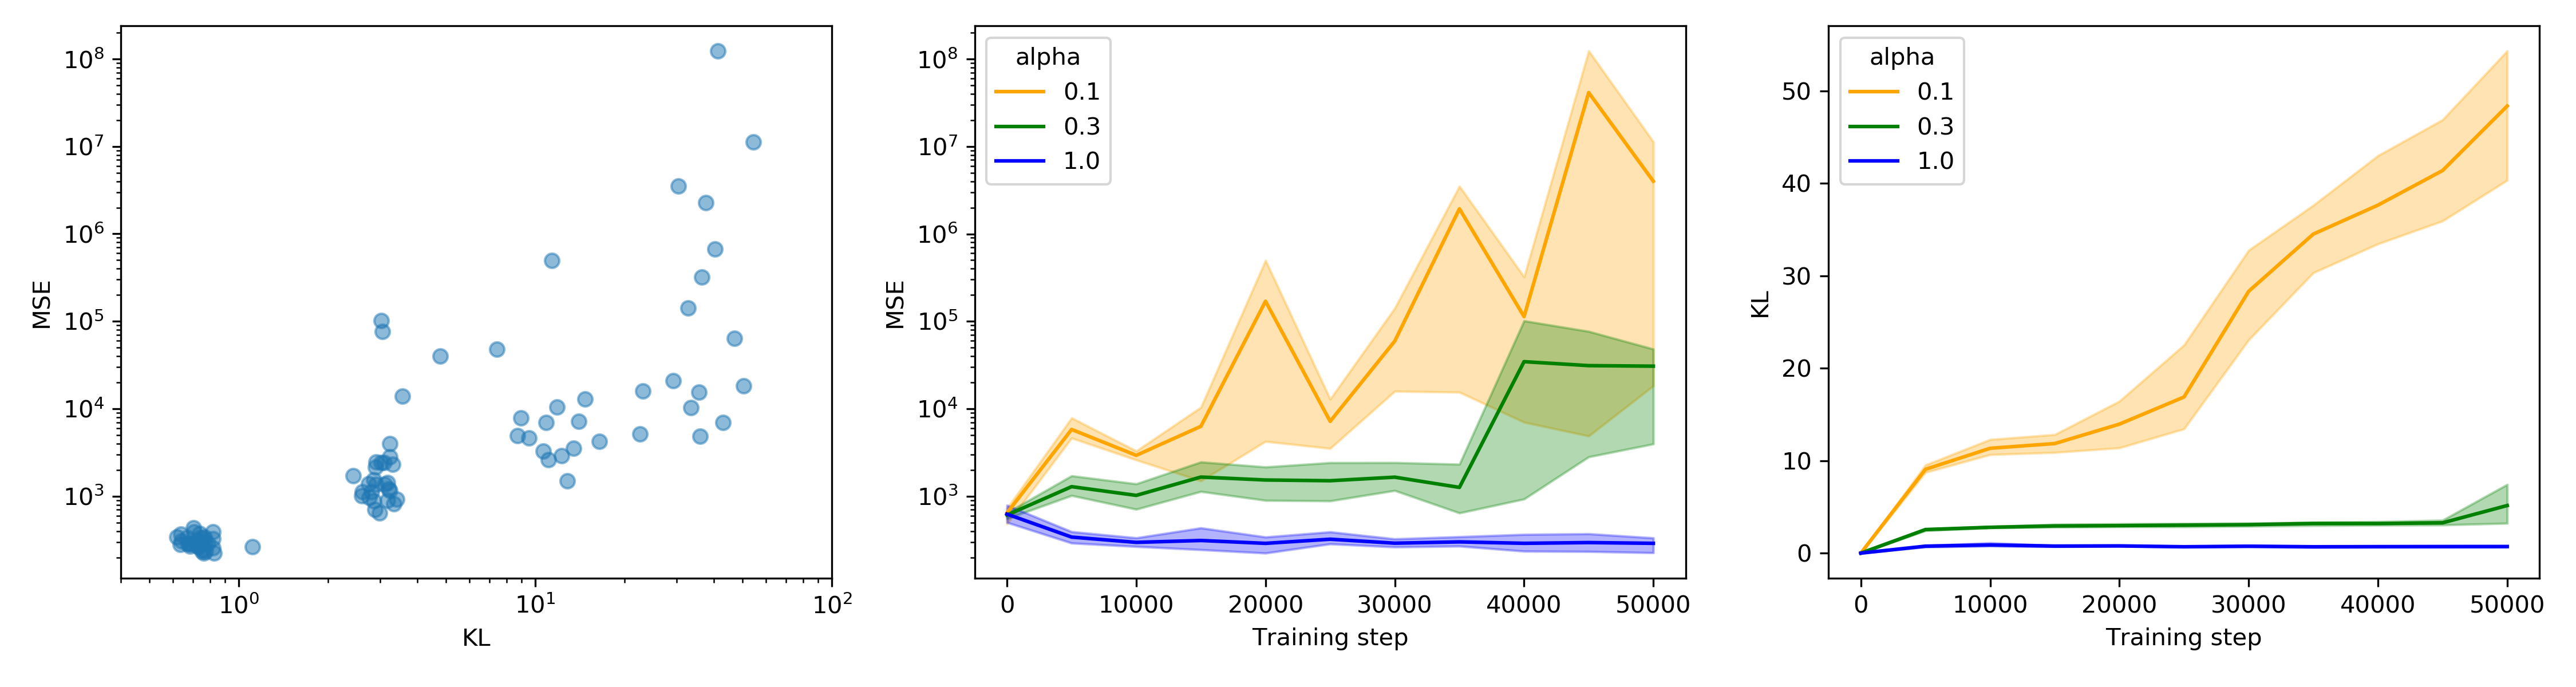
\includegraphics[width=\textwidth]{figures/offline-rl/mse/mse_vs_kl.png}
    \caption{Results of running the iterative algorithm on halfcheetah-medium. Each checkpointed policy is evaluated by a Q function trained from scratch on heldout data. MSE refers to $\E_{s,a\sim \beta}[\hat Q^{\pi_i}(s,a) - Q^{\pi_i}(s,a)]$ and KL refers to $ \E_{s\sim \beta}[KL(\pi(\cdot|s)\| \beta(\cdot|s)]$. Left: 90 policies taken from various points in training with various hyperaparmeters and random seeds. Center: MSE learning curves. Right: KL learning curves. Error bars show min and max over 3 random seeds.}
    \label{fig:mse}
\end{figure}


\subsection{Iterative error exploitation}

The previous subsection identifies how any algorithm that uses off-policy evaluation is fundamentally limited by distribution shift, even if we were given fresh data and trained Q functions from scratch at every iteration. But, in practice, iterative algorithms repeatedly iterate between optimizing policies against estimated Q functions and re-estimating the Q functions using the \emph{same data} and using the Q function from the previous step to warm-start the re-estimation. This induces dependence between steps that causes a problem that we call iterative error exploitation.


\paragraph{Intuition about the problem.} In short, iterative error exploitation happens because $ \pi_i$ tends to choose overestimated actions in the policy improvement step, and then this overestimation propagates via dynamic programming in the policy evaluation step. To illustrate this issue more formally, consider the following: at each $ s,a$ we suffer some Bellman error $ \varepsilon_\beta^\pi(s,a)$ based on our fixed dataset collected by $ \beta$. Formally,
\begin{align}
    \widehat Q^\pi(s,a) = r(s,a) + \gamma \E_{\substack{s'|s,a \\ a'\sim \pi|s'}}[\widehat Q^\pi(s',a')] + \varepsilon_\beta^\pi(s,a).
\end{align}
Intuitively, $ \varepsilon_\beta^\pi$ will be larger at state-actions with less coverage in the dataset collected by $ \beta$. Note that $ \varepsilon_\beta^\pi $ can absorb all noise due to our finite dataset as well as function approximation error.

%So far this is all fully general, such an $ \varepsilon_\beta^\pi$ can always be defined for any estimated Q function. Now we will make the simplifying assumption.
All that is needed to cause iterative error exploitation is that the $ \epsilon_\beta^\pi$ are highly correlated across different $ \pi$, but for simplicity, we will assume that $ \varepsilon_\beta^\pi$ is \emph{the same} for all policies $ \pi$ estimated from our fixed offline dataset and instead write $ \varepsilon_\beta$. Now that the errors do not depend on the policy we can treat the errors as auxiliary rewards that obscure the true rewards and see that
\begin{align}
    \widehat Q^\pi(s,a) = Q^\pi(s,a) + \widetilde Q^\pi_\beta(s,a), \qquad \widetilde Q^\pi_\beta(s,a) := \E_{\pi| s_0, a_0 = s,a }\left[\sum_{t=0}^\infty \gamma^t \varepsilon_\beta(s_t,a_t) \right].
\end{align}
This assumption is somewhat reasonable since we expect the error to primarily depend on the data. And, when the prior Q function is used to warm-start the current one (as is generally the case in practice), the approximation errors are automatically passed between steps.

Now we can explain the problem. Recall that under our assumption the $ \varepsilon_\beta $ are fixed once we have a dataset and likely to have larger magnitude the further we go from the support of the dataset. So, with each step $ \pi_i$ is able to better maximize $ \varepsilon_\beta$, thus moving further from $ \beta$ and increasing the magnitude of $ \widetilde Q^{\pi_i}_\beta$ relative to $ Q^{\pi_i}$. Even though $ Q^{\pi_i}$ may provide better signal than $ Q^\beta$, it can easily be drowned out by $ \widetilde Q^{\pi_i}_\beta$. In contrast, $ \widetilde Q_\beta^\beta$ has small magnitude, so the one-step algorithm is robust to errors\endnote{We should note that iterative error exploitation is similar to the overestimation addressed by double Q learning \citep{van2016deep, fujimoto2018addressing}, but distinct. Since we are in the offline setting, the errors due to our finite dataset can be iteratively exploited more and more, while in the online setting considered by double Q learning, fresh data prevents this issue. We are also considering an algorithm based on policy iteration rather than value iteration.}.

\paragraph{An example.} Now we consider a simple gridworld example to illustrate iterative error exploitation. This example fits exactly into the setup outlined above since all errors are due to reward estimation so the $ \varepsilon_\beta$ is indeed constant over all $ \pi$. The gridworld we consider has one deterministic good state with reward 1 and many stochastic bad states that have rewards distributed as $ \mathcal{N}(-0.5, 1)$. We collect a dataset of 100 trajectories, each of length 100. One run of the multi-step offline regularized policy iteration algorithm is illustrated in Figure \ref{fig:gridworld}.

\begin{figure}[h]
    \centering
    %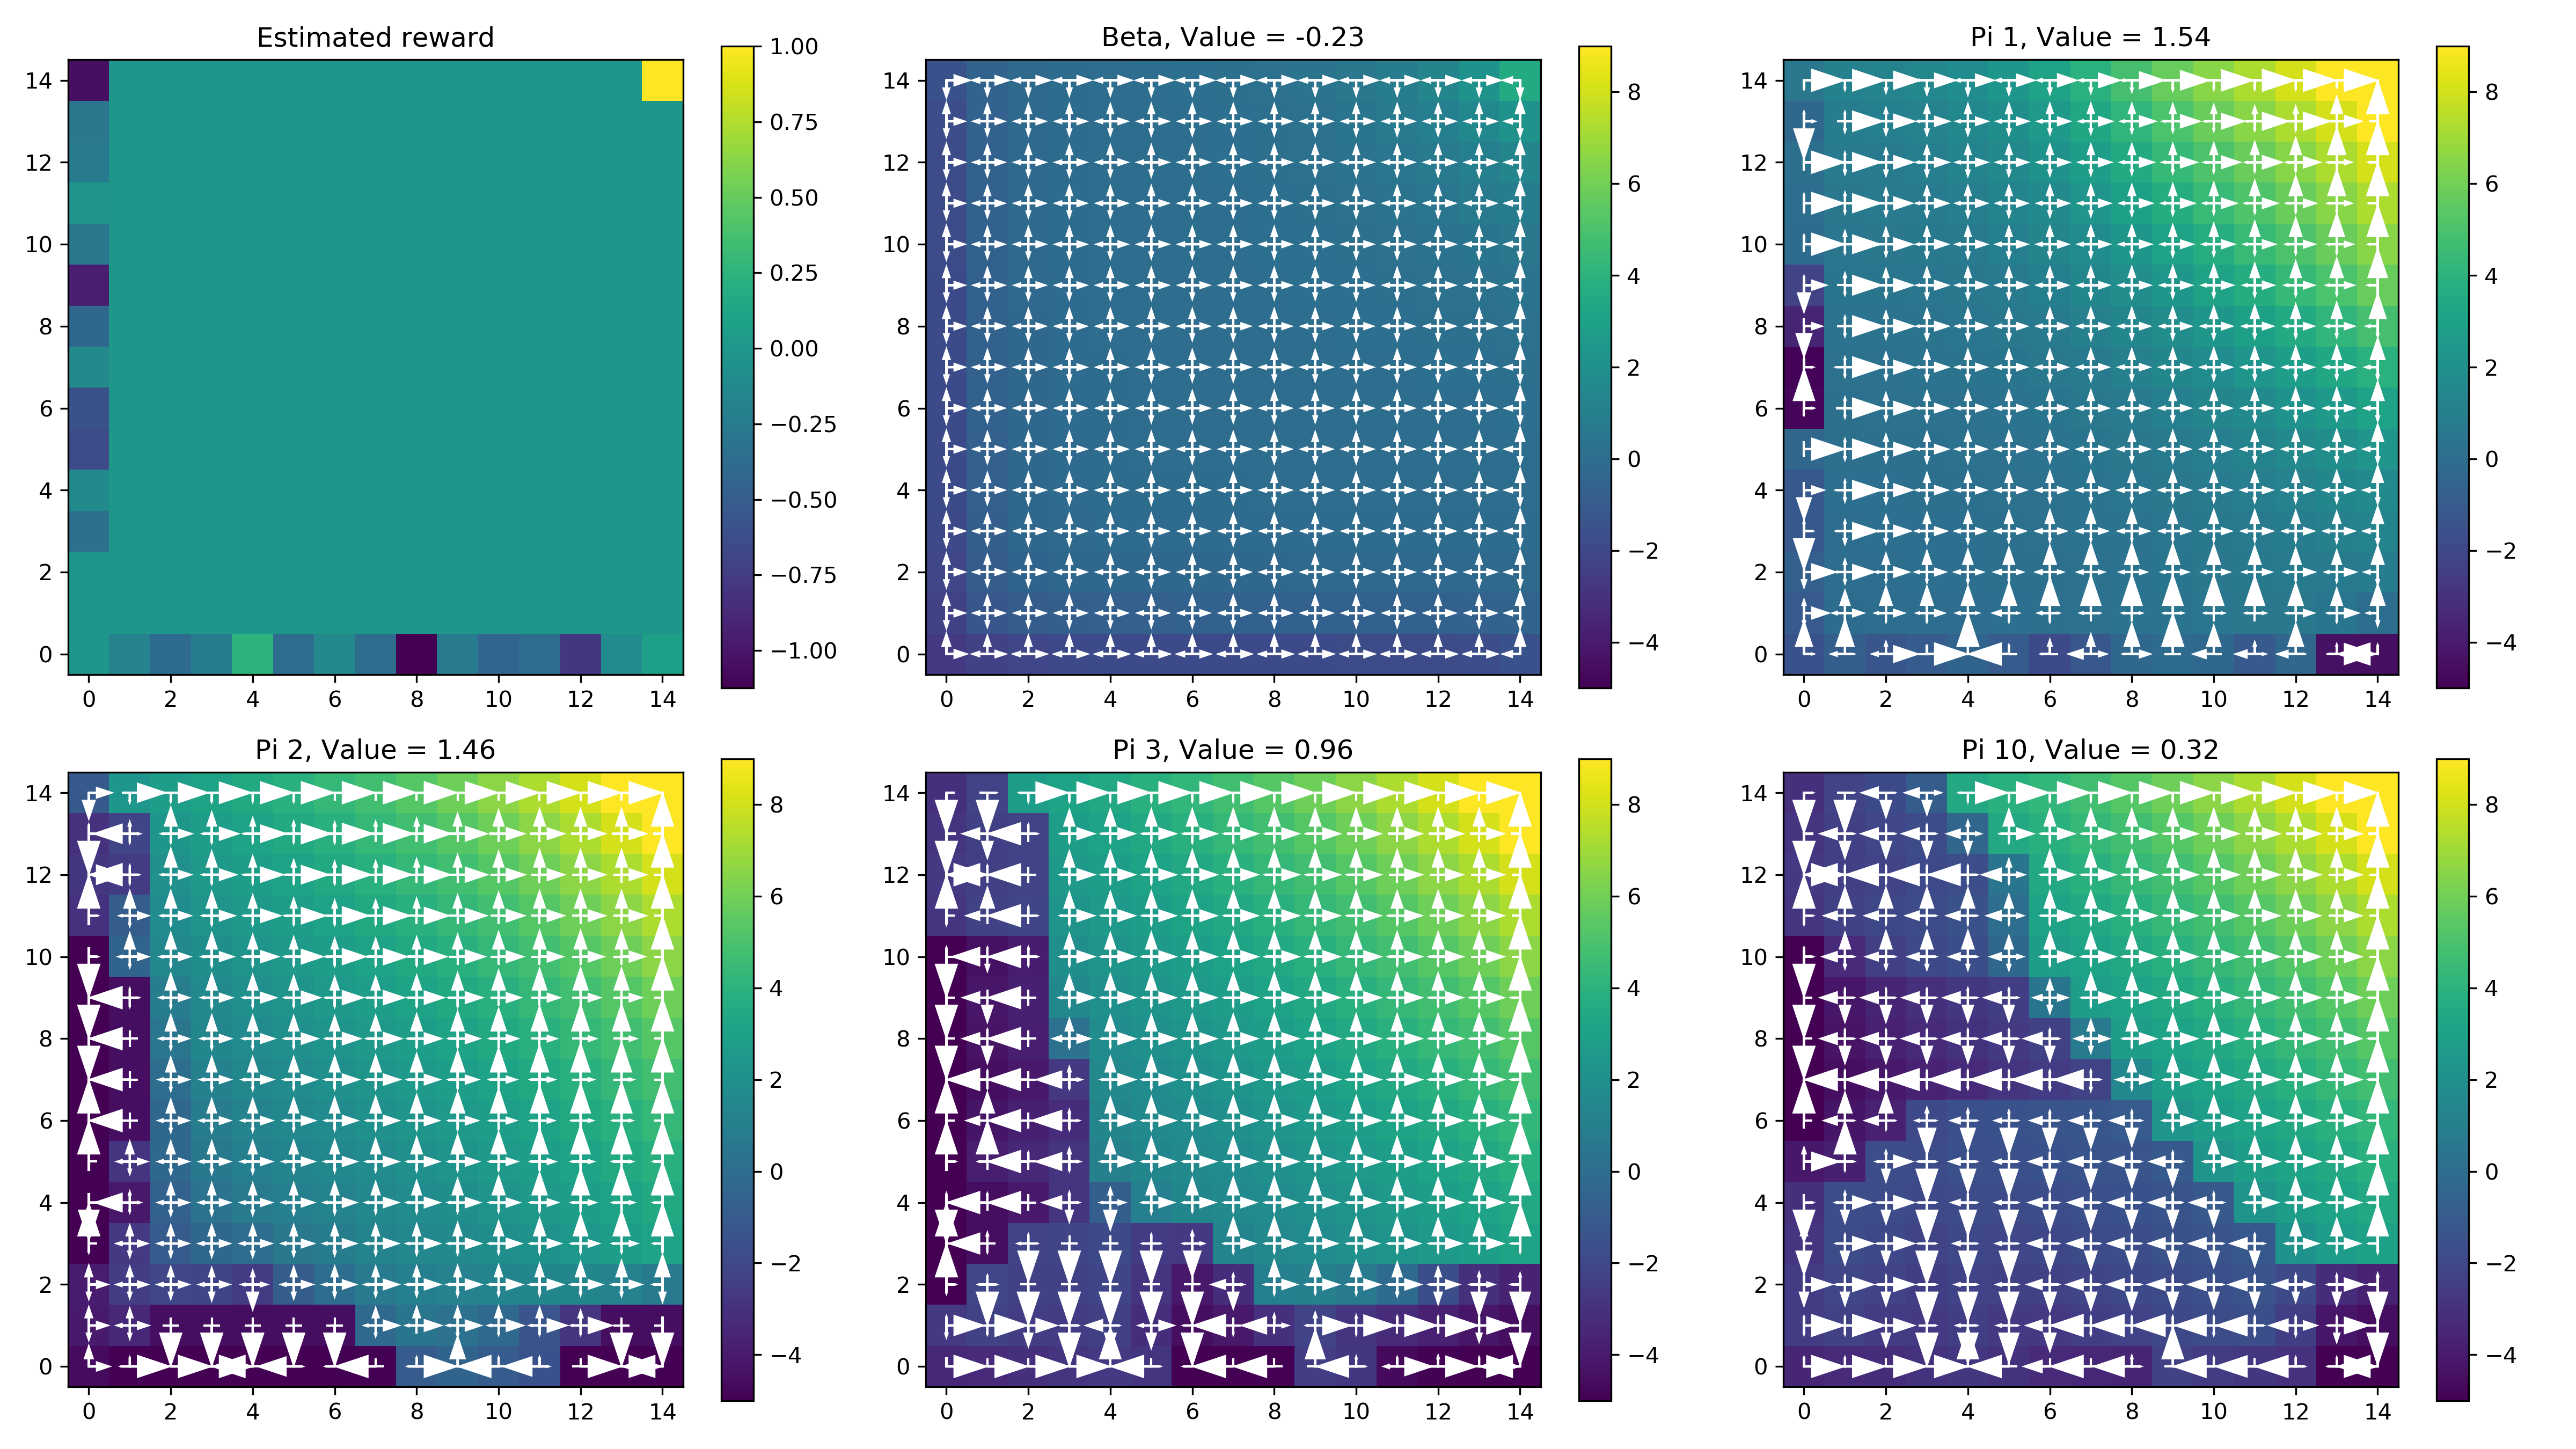
\includegraphics[width = 0.8\textwidth]{figures/offline-rl/gridworld/gridworld_onestep.png}
    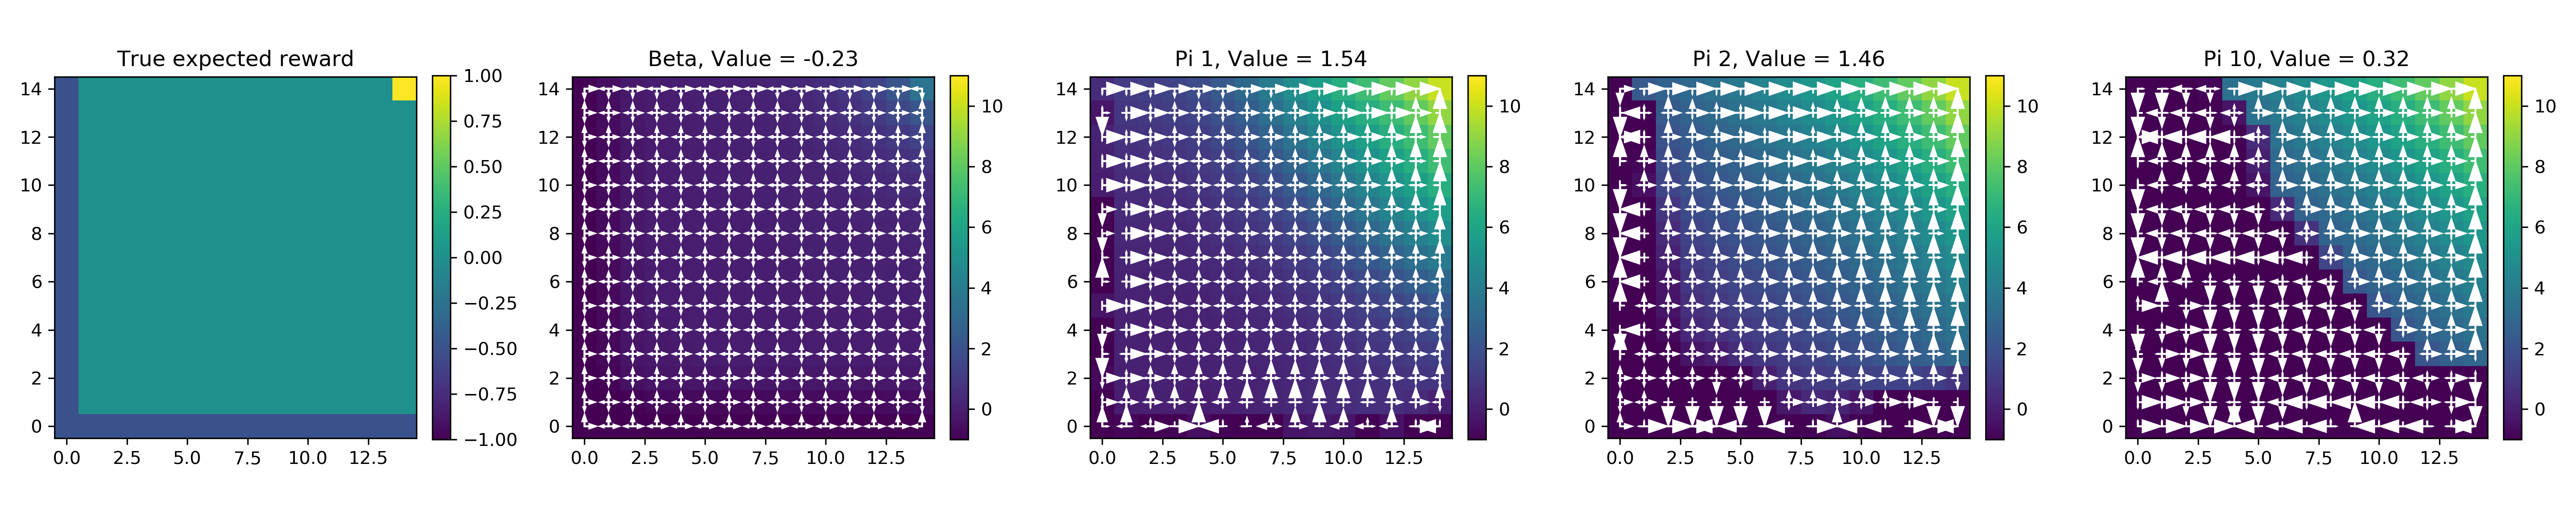
\includegraphics[width=\textwidth]{figures/offline-rl/gridworld/gridworld_flat.png}
    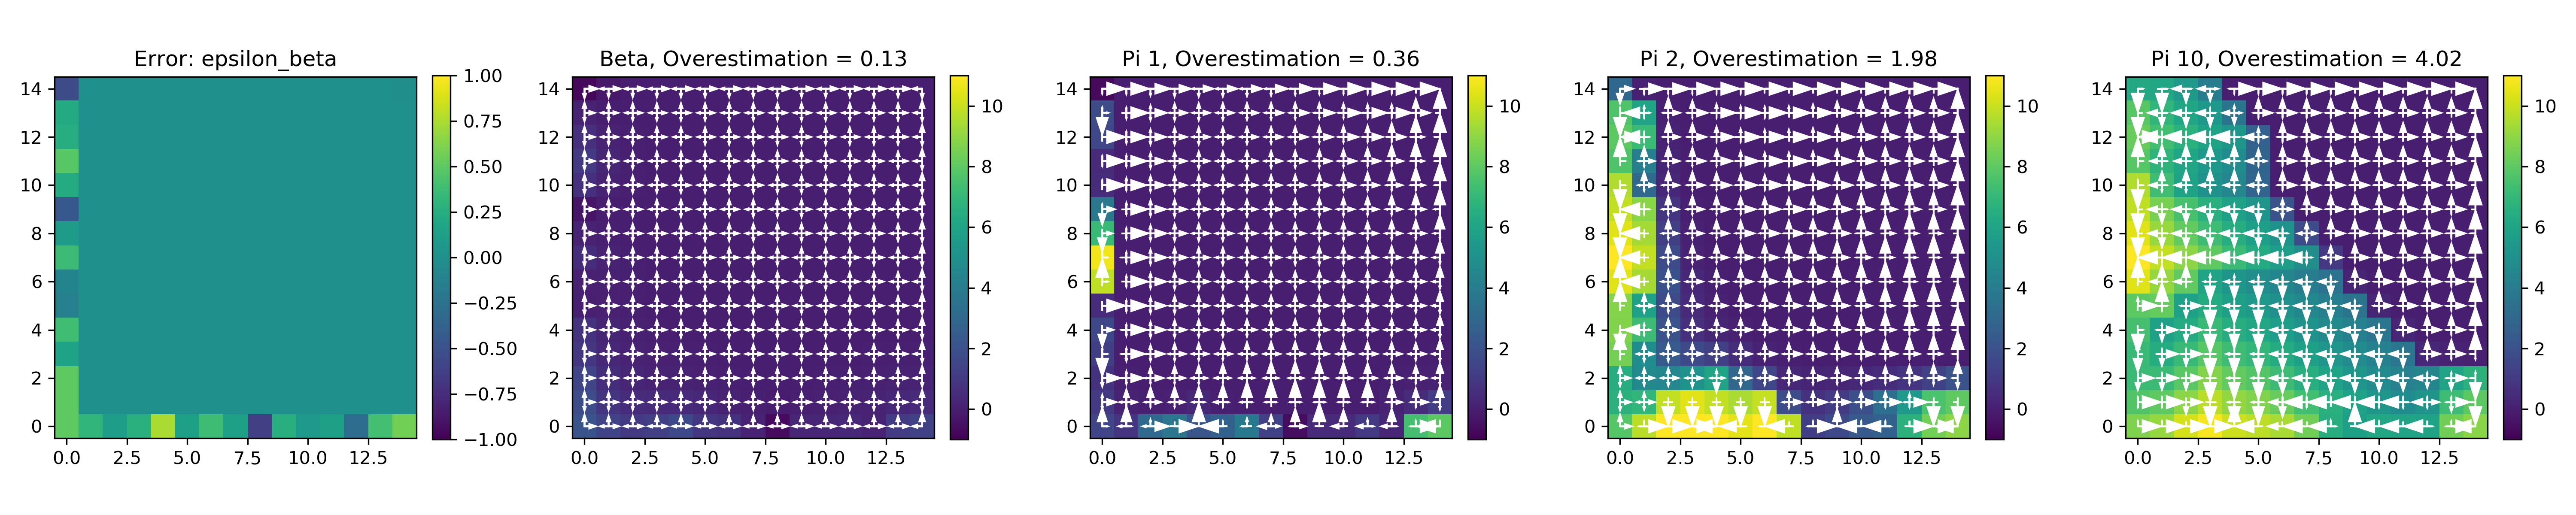
\includegraphics[width=\textwidth]{figures/offline-rl/gridworld/gridworld_error.png}
    \caption{An illustration of multi-step offline regularized policy iteration. The leftmost panel in each row shows the true reward (top) or error $ \varepsilon_\beta$ (bottom). Then each subsequent panel plots $ \pi_i$ (with arrow size proportional to $ \pi_i(a|s)$) over either $ Q^{\pi_i}$ (top) or $ \widetilde Q^{\pi}_\beta $ (bottom), averaged over actions at each state. The one-step policy ($ \pi_1$) has the highest value. The behavior policy here is a mixture of optimal $ \pi^*$ and uniform $ u $ with coefficient 0.2 so that $\beta = 0.2 \cdot \pi^* + 0.8 \cdot u$. We set $ \alpha = 0.1$ as the regularization parameter for reverse KL regularization.}
    \label{fig:gridworld}
\end{figure}


In the example, like in the D4RL benchmark, we see that one step outperforms multiple steps of improvement. Intuitively, when there are so many noisy states, it is likely that a few of them will be overestimated. Since the data is re-used for each step, these overestimations persist and propagate across the state space due to iterative error exploitation. This property of having many bad, but poorly estimated states likely also exists in the high-dimensional control problems encountered in the benchmark where there are many ways for the robots to fall down that are not observed in the data for non-random behavior.
\begin{figure}[h]
\vspace{-0.5cm}
    \centering
    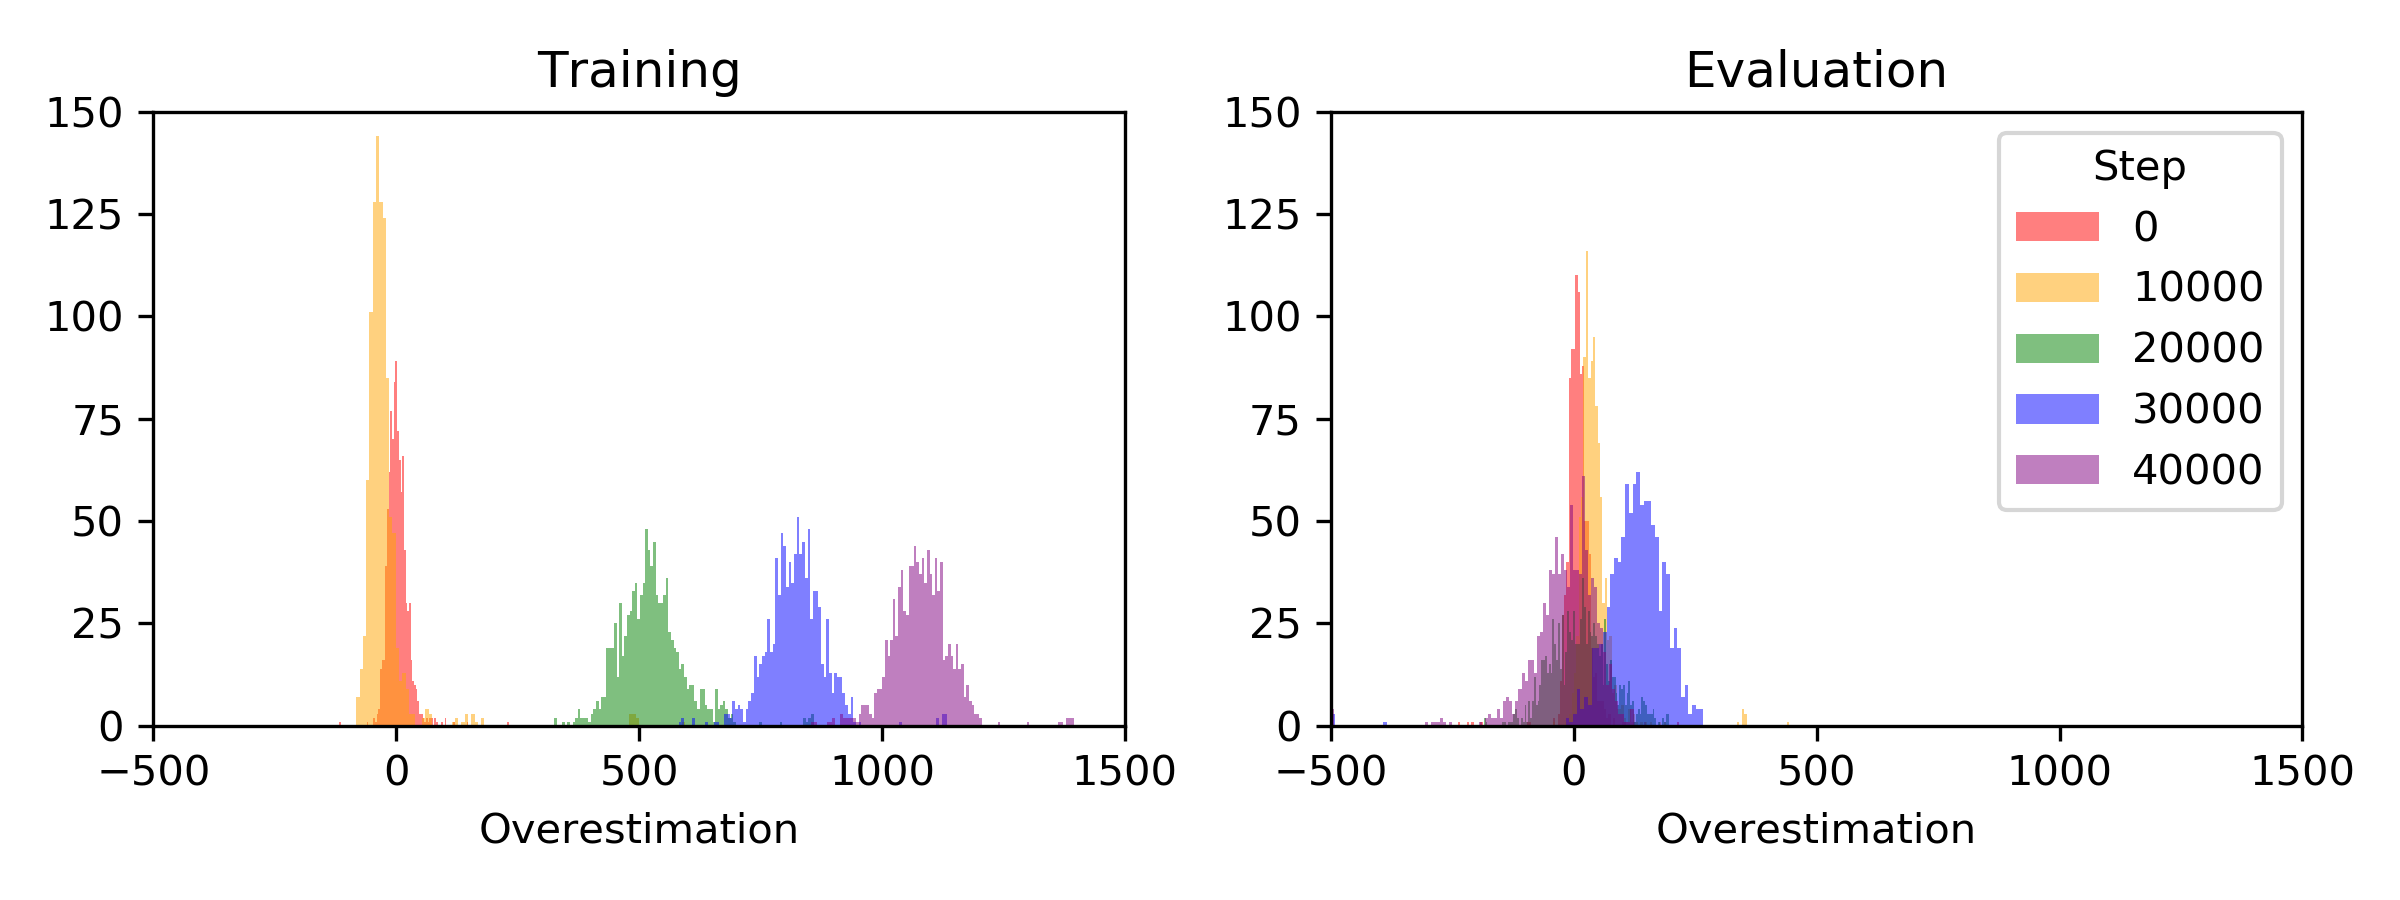
\includegraphics[width=0.6\textwidth]{figures/offline-rl/estimation/histograms.png}
    \caption{Histograms of overestimation error ($\widehat Q^{\pi_i}(s,a) - Q^{\pi_i}(s,a)$) on halfcheetah-medium with the iterative algorithm. Left: errors from the training Q function. Right: errors from an independently trained Q function.}
    \label{fig:over}
\end{figure}
Moreover, both settings have larger errors in areas where we have less data.
So even though the errors in the gridworld are caused by noise in the rewards, while errors in D4RL are caused by function approximation, we think this is a useful mental model of the problem.

\paragraph{Empirical evidence.}
In practice we cannot easily visualize the progression of errors. However, the dependence between steps still arises as overestimation of the Q values. We can track the overestimation of the Q values over training as a way to measure how much bias is being induced by optimizing against our dependent Q estimators. As a control we can also train Q estimators from scratch on independently sampled evaluation data. These independently trained Q functions do not have the same overestimation bias even though the squared error does tend to increase as the policy moves further from the behavior (as seen in Figure \ref{fig:mse}).
Explicitly, we track 1000 state, action pairs from the replay buffer over training. For each checkpointed policy we perform 3 rollouts at each state to get an estimate of the true Q value and compare this to the estimated Q value. Results are shown in Figure \ref{fig:over}.








\section{When are multiple steps useful?}\label{sec:when}

So far we have focused on why the one-step algorithm often works better than the multi-step and iterative algorithms. However, we do not want to give the impression that one-step is always better. Indeed, our own experiments in Section \ref{sec:bench} show a clear advantage for the multi-step and iterative approaches when we have randomly collected data. While we cannot offer a precise delineation of when one-step will outperform multi-step, in this section we offer some intuition as to when we can expect to see benefits from multiple steps of policy improvement.

As seen in Section~\ref{sec:why}, multi-step and iterative algorithms have problems when they propagate estimation errors. This is especially problematic in noisy and/or high dimensional environments. While the multi-step algorithms propagate this noise more widely than the one-step algorithm, they also propagate the signal. So, when we have sufficient coverage to reduce the magnitude of the noise, this increased propagation of signal can be beneficial. The D4RL experiments suggest that we are usually on the side of the tradeoff where the errors are large enough to make one-step preferable.


\begin{figure}[h]
\vspace{-0.3cm}
    \centering
    \includegraphics[width=0.4\textwidth]{figures/offline-rl/learning curves/r-m_mixture.png}
    \caption{Performance of all three algorithms with reverse KL regularization across mixtures between halfcheetah-random and halfcheetah-medium. Error bars indicate min and max over 3 seeds.}
    \label{fig:interp}
\end{figure}

In Appendix~\ref{sec:app_grid} we illustrate a simple gridworld example where a slight modification of the behavior policy from Figure~\ref{fig:gridworld} makes multi-step dramatically outperform one-step. This modified behavior policy (1) has better coverage of the noisy states (which reduces error, helping multi-step), and (2) does a worse job propagating the reward from the good state (hurting one-step).

We can also test empirically how the behavior policy effects the tradeoff between error and signal propagation. To do this we construct a simple experiment where we mix data from the random behavior policy with data from the medium behavior policy. Explicitly we construct a dataset $ D $ out of the datasets $ D_r$ for random and $ D_m$ for medium such that each trajectory in $ D $ comes from the medium dataset with probability $ p_m$. So for $ p_m = 0$ we have the random dataset and $ p_m = 1 $ we have the medium dataset, and in between we have various mixtures. Results are shown in Figure~\ref{fig:interp}. It takes surprisingly little data from the medium policy for one-step to outperform the iterative algorithm.



\section{Discussion, limitations, and future work}

This paper presents the surprising effectiveness of a simple one-step baseline for offline RL. We examine the failure modes of iterative algorithms and the conditions where we might expect them to outperform the simple one-step baseline. This provides guidance to a practitioner that the simple one-step baseline is a good place to start when approaching an offline RL problem.

But, we leave many questions unanswered.
One main limitation is that we lack a clear theoretical characterization of which environments and behaviors can guarantee that one-step outperforms multi-step or visa versa. Such results will likely require strong assumptions, but could provide useful insight. We don't expect this to be easy as it requires understanding policy iteration which has been notoriously difficult to analyze, often converging much faster than the theory would suggest \citep{sutton2018reinforcement, Agarwal2019ReinforcementLT}.
Another limitation is that while only using one step is perhaps the simplest way to avoid the problems of off-policy evaluation, there are possibly other more elaborate algorithmic solutions that we did not consider here. However, our strong empirical results suggest that the one-step algorithm is at least a strong baseline.









\clearpage
\begin{subappendices}
\newappendix{Gridworld example where multi-step outperforms one-step}\label{sec:app_grid}

As explained in the main text, this section presents an example that is only a slight modification of the one in Figure \ref{fig:gridworld}, but where a multi-step approach is clearly preferred over just one step. The data-generating and learning processes are exactly the same (100 trajectories of length 100, discount 0.9, $ \alpha = 0.1$ for reverse KL regularization). The only difference is that rather than using a behavior that is a mixture of optimal and uniform, we use a behavior that is a mixture of maximally suboptimal and uniform. If we call the suboptimal policy $ \pi^-$ (which always goes down and left in our gridworld), then the behavior for the modified example is $ \beta = 0.2 \cdot \pi^- + 0.8 \cdot u$, where $ u $ is uniform. Results are shown in Figure \ref{fig:multi_gridworld}.

\begin{figure}[h]
    \centering
    \includegraphics[width=\textwidth]{figures/offline-rl/gridworld/multi_gridworld_flat.png}
    \includegraphics[width=\textwidth]{figures/offline-rl/gridworld/multi_gridworld_error.png}
    \caption{A gridworld example with modified behavior where multi-step is much better than one-step.}
    \label{fig:multi_gridworld}
\end{figure}

By being more likely to go to the noisy states, this behavior policy allows us to get lower variance estimates of the rewards. Essentially, the coverage of the behavior policy in this example reduces the magnitude of the evaluation errors. This allows for more aggressive planning using multi-step methods. Moreover, since the behavior is less likely to go to the good state, the behavior Q function does not propagate the signal from the rewarding state as far, harming the one-step method.

\newappendix{Connection to policy improvement guarantees}\label{sec:app_improvement}


The regularized or constrained one-step algorithm performs an update that directly inherits guarantees from the literature on conservative policy improvement \citep{kakade2002approximately, schulman2015trust, achiam2017constrained}. These original papers consider an online setting where more data is collected at each step, but the guarantee at each step applies to our one-step offline algorithm.

The key idea of this line of work begins with the performance difference lemma of \cite{kakade2002approximately}, and then lower bounds the amount of improvement over the behavior policy. Define the discounted state visitation distribution for a policy $ \pi$ by $ d^\pi(s) := (1-\gamma) \sum_{t=0}^\infty \gamma^t \Prob_{\rho, P, \pi}(s_t = s)$. We will also use the shorthand $ Q(s, \pi) $ to denote $ \E_{a\sim\pi|s}[Q(s,a)]$. Then we have the performance difference lemma as follows.

\begin{lemma}[Performance difference, \cite{kakade2002approximately}]
For any two policies $ \pi$ and $ \beta$,
\begin{align}
    J(\pi) - J(\beta) = \frac{1}{1-\gamma} \E_{\substack{s \sim d^\pi}}[ Q^\beta(s,\pi) - Q^\beta(s, \beta)]. %:= \frac{1}{1-\gamma} \E_{\substack{s \sim d_\pi }}[ A^\beta_\pi(s)].
\end{align}
\end{lemma}

Then, Corollary 1 from \cite{achiam2017constrained} (reproduced below) gives a guarantee for the one-step algorithm. The key idea is that when $ \pi $ is sufficiently close to $ \beta$, we can use $ Q^\beta$ as an approximation to $ Q^\pi$.
\begin{lemma}[Conservative Policy Improvement, \cite{achiam2017constrained}]
For any two policies $ \pi$ and $ \beta$, let $ \|A^\beta_\pi\|_{\infty} = \sup_s  |Q^\beta(s,\pi) - Q^\beta(s, \beta)|$. Then,
    \begin{align}
        J(\pi) - J(\beta) \geq \frac{1}{1-\gamma} \E_{\substack{s \sim d^\beta}}\left[ \left(Q^\beta(s,\pi) - Q^\beta(s, \beta)\right) - \frac{2\gamma \|A^\beta_\pi\|_\infty}{1-\gamma} D_{TV}(\pi(\cdot|s)\|\beta(\cdot|s)) \right]
    \end{align}
where $ D_{TV}$ denotes the total variation distance.
\end{lemma}

Replacing $ Q^\beta$ with $ \widehat Q^\beta$ and the TV distance by the KL, we get precisely the objective that we optimize in the one-step algorithm. This shows that the one-step algorithm indeed optimizes a lower bound on the performance difference. Of course, in practice we replace the potentially large multiplier on the divergence term by a hyperparameter, but this theory at least motivates the soundness of the approach.

We are not familiar with similar guarantees for the iterative or multi-step approaches that rely on off-policy evaluation.


\newappendix{Experimental setup}\label{sec:app_exp_setup}

\subsection{Benchmark experiments (Tables \ref{tab:d4rl} and \ref{tab:multi}, Figure \ref{fig:learning_curves})}

\paragraph{Data.} We use the datasets from the D4RL benchmark \citep{fu2020d4rl}. We use the latest versions, which are v2 for the mujoco datasets and v1 for the adroit datasets.

\paragraph{Hyperparameter tuning.}
\begin{table}[ht]
\vspace{-0.2cm}
    \centering
    \caption{Hyperparameter sweeps for each algorithm.}
    \begin{small}
    \begin{tabular}{lc}
        \toprule
        Algorithm & Hyperparameter set \\
        \midrule
        Reverse KL ($ \alpha$) &
                    \{0.03, 0.1, 0.3, 1.0, 3.0, 10.0\}\\
        Easy BCQ ($ M$) &
                    \{2, 5, 10, 20, 50, 100\}\\
        Exponentially weighted ($ \tau$) &
                    \{0.1, 0.3, 1.0, 3.0, 10.0, 30.0\}\\
        \bottomrule
    \end{tabular}
    \end{small}
    \label{tab:hyperparams}
\end{table}
We follow the practice of \cite{fu2020d4rl} and tune a small set of hyperparameters by interacting with the simulator to estimate the value of the policies learned under each hyperparameter setting. The hyperparameter sets for each algorithm can be seen in Table \ref{tab:hyperparams}.

This may initially seem like ``cheating'', but can be a reasonable setup if we are considering applications like robotics where we can feasibly test a small number of trained policies on the real system. Also, since prior work has used this setup, it makes it easiest to compare our results if we use it too. While beyond the scope of this work, we do think that better offline model selection procedures will be crucial to make offline RL more broadly applicable. A good primer on this topic can be found in \cite{paine2020hyperparameter}.


\paragraph{Models.} All of our Q functions and policies are simple MLPs with ReLU activations and 2 hidden layers of width 1024. Our policies output a truncated normal distribution with diagonal covariance where we can get reparameterized samples by sampling from a uniform distribution and computing the differentiable inverse CDF \citep{Burkhardt2014truncated}. We found this to be more stable than the tanh of normal used by e.g. \cite{fu2020d4rl}, but to achieve similar performance when both are stable. We use these same models across all experiments.


\paragraph{One-step training procedure.} For all of our one-step algorithms, we train our $ \hat \beta $ behavior estimate by imitation learning for 500k gradient steps using Adam \citep{kingma2014adam} with learning rate 1e-4 and batch size 512. We train our $ \widehat Q^\beta$ estimator by fitted Q evaluation with a target network for 2 million gradient steps using Adam with learning rate 1e-4 and batch size 512. The target is updated softly at every step with parameter $ \tau = 0.005$. All policies are trained for 100k steps again with Adam using learning rate 1e-4 and batch size 512.

Easy BCQ does not require training a policy network and just uses $ \hat \beta$ and $ \widehat Q^\beta$ to define it's policy. For the exponentially weighted algorithm, we clip the weights at 100 to prevent numerical instability. To estimate reverse KL at some state we use 10 samples from the current policy and the density defined by our estimated $ \hat \beta$.

Each random seed retrains all three models (behavior, Q, policy) from different initializations. We use three random seeds.

\paragraph{Multi-step training procedure.} For multi-step algorithms we use all the same hyperparameters as one-step. We initialize our policy and Q function from the same pre-trained $ \hat \beta$ and $ \widehat Q^\beta$ as we use for the one-step algorithm trained for 500k and 2 million steps respectively. Then we consider 5 policy steps. To ensure that we use the same number of gradient updates on the policy, each step consists of 20k gradient steps on the policy followed by 200k gradient steps on the Q function. Thus, we take the same 100k gradient steps on the policy network. Now the Q updates are off-policy so the next action $a'$ is sampled from the current policy $ \pi_i$ rather than from the dataset.

\paragraph{Iterative training procedure.} For iterative algorithms we again use all the same hyperparameters and initialize from the same $ \hat \beta$ and $ \widehat Q^\beta$. We again take the same 100k gradient steps on the policy network. For each step on the policy network we take 2 off-policy gradient steps on the Q network.



\paragraph{Evaluation procedure.} To evaluate each policy we run 100 trajectories in the environment and compute the mean. We then report the mean and standard deviation over three training seeds.




\subsection{MSE experiment (Figure 3)}

\paragraph{Data.} To get an independently sampled dataset of the same size as the training set, we use the behavior cloned policy $ \hat \beta$ to sample 1000 trajectories. The checkpointed policies are taken at intervals of 5000 gradient steps from each of the three training seeds.

\paragraph{Training procedure.} The $\widehat Q^{\pi_i}$ training procedure is the same as before so we use Adam with step size 1e-4 and batch size 512 and a target network with soft updates with parameter 0.005. We train for 1 million steps.

\paragraph{Evaluation procedure.} To evaluate MSE, we sample 1000 state, action pairs from the original training set and from each state, action pair we run 3 rollouts. We take the mean over the rollouts and then compute squared error at each state, action pair and finally get MSE by taking the mean over state, action pairs. The reported reverse KL is evaluated by samples during training. At each state in a batch we take 10 samples to estimate the KL at that state and then take the mean over the batch.


\subsection{Gridworld experiment (Figure 4)}

\paragraph{Environment.} The environment is a 15 x 15 gridworld with deterministic transitions. The rewards are deterministically 1 for all actions taken from the state in the top right corner and stochastic with distribution $ \mathcal{N}(-0.5, 1)$ for all actions taken from states on the left or bottom walls. The initial state is uniformly random. The discount is 0.9.

\paragraph{Data.} We collect data from a behavior policy that is a mixture of the uniform policy (with probability 0.8) and an optimal policy (with probability 0.2). We collect 100 trajectories of length 100.

\paragraph{Training procedure.} We give the agent access to the deterministic transitions. The only thing for the agent to do is estimate the rewards from the data and then learn in the empirical MDP. We perform tabular Q evaluation by dynamic programming. We initialize with the empirical rewards and do 100 steps of dynamic programming with discount 0.9. Regularized policy updates are solved for exactly by setting $ \pi_i(a|s) \propto \beta(a|s) \exp(\frac{1}{\alpha} \widehat Q^{\pi_{i-1}}(s,a))$.




\subsection{Overestimation experiment (Figure 5)}

This experiment uses the same setup as the MSE experiment. The main difference is we also consider the Q functions learned during training and demonstrate the overestimation relative to the Q functions trained on the evaluation dataset as in the MSE experiment.


\subsection{Mixed data experiment (Figure 6)}

We construct datasets with $ p_m = \{0.0, 0.1, 0.2, 0.4, 0.6, 0.8, 1.0\}$ by mixing the random and medium datasets from D4RL and then run the same training procedure as we did for the benchmark experiments. Each dataset has the same size, but a different proportion of trajectories from the medium policy.


\newappendix{Learning curves}\label{sec:app_extra_exp}

In this section we reproduce the learning curves and hyperparameter plots across the one-step, multi-step, and iterative algorithms with reverse KL regularization, as in Figure \ref{fig:learning_curves}.

\vspace{-0.2cm}
\begin{figure}[h]
    \centering
    \includegraphics[width=0.85\textwidth]{figures/offline-rl/learning curves/lc-halfcheetah-medium-v2.png}
    \includegraphics[width=0.85\textwidth]{figures/offline-rl/learning curves/lc-walker2d-medium-v2.png}
    \includegraphics[width=0.85\textwidth]{figures/offline-rl/learning curves/lc-hopper-medium-v2.png}
    \vspace{-0.2cm}
    \caption{Learning curves on the medium datasets.}
    \label{fig:app_lc_medium}
\end{figure}


\begin{figure}[h]
    \centering
    \includegraphics[width=0.85\textwidth]{figures/offline-rl/learning curves/lc-halfcheetah-medium-expert-v2.png}
    \includegraphics[width=0.85\textwidth]{figures/offline-rl/learning curves/lc-walker2d-medium-expert-v2.png}
    \includegraphics[width=0.85\textwidth]{figures/offline-rl/learning curves/lc-hopper-medium-expert-v2.png}
    \vspace{-0.2cm}
    \caption{Learning curves on the medium-expert datasets.}
    \label{fig:app_lc_medium-expert}
\end{figure}


\begin{figure}[h]
    \centering
    \includegraphics[width=0.85\textwidth]{figures/offline-rl/learning curves/lc-halfcheetah-random-v2.png}
    \includegraphics[width=0.85\textwidth]{figures/offline-rl/learning curves/lc-walker2d-random-v2.png}
    \includegraphics[width=0.85\textwidth]{figures/offline-rl/learning curves/lc-hopper-random-v2.png}
    \vspace{-0.2cm}
    \caption{Learning curves on the random datasets.}
    \label{fig:app_lc_random}
\end{figure}
\end{subappendices}



\printendnotes


\chapter{Conclusion} \label{sec:conclusion}
For reinforcement learning to be practical to use on physical systems such as robots, there is no property more important than sample efficiency.
The work contained in this thesis represents a small step towards RL algorithms for robotic control that require less data collection.
\Cref{sec:exploration} proposed a new technique for collecting diverse data more rapidly while simultaneously approximating the optimal policy.
\Cref{sec:representation} described the role of representation and inductive bias in machine learning and proposed a representation learning objective specifically designed to improve sample efficiency in reinforcement learning.
\Cref{sec:offline} studied the problem of finding as good a policy as possible given a fixed dataset, examining the limits of reinforcement learning without data collection.
These represent three different thrusts towards sample-efficient RL: collecting more informative data, using representations to generalize better, and learning policies without collecting data at all.

From here there are many exciting future directions.
Using the decoupled policy learning technique from \Cref{sec:deep}, alternative exploration bonuses could capture prior knowledge about a task or environment without biasing the final policy.
This could lead to significantly more directed exploration, overcoming the need to visit every possible transition in an MDP.

Representation learning for reinforcement learning has seen a flurry of progress after the publication of \Cref{sec:dyne}.
Contrastive methods have seen significant success using explicit representation learning or implicitly via data augmentation \citep{Srinivas2020CURLCU,laskin2020reinforcement,Kostrikov2021ImageAI}.
Representation learning based on causal principles and invariances have also resulted in intriguing possibilities \citep{Zhang2020InvariantCP,Zhang2021LearningIR}.
A major limitation of the representations learned in \Cref{sec:dyne} is that they are trained on data coming from a uniformly random behavior policy; by using directed exploration, better representations can be learned, as proposed in \citep{Yarats2021ReinforcementLW}.

The batched single-step policy improvement operator discussed in \Cref{sec:offline-rl} is conservative, and thus on its own not ideally suited for settings with data collection.
However, by coupling it with an efficient directed exploration technique such as the one proposed in \Cref{sec:deep}, such a conservative policy improvement could lead to better policy performance on limited data.
Future work may also tackle the problem of accumulating error with iterative policy optimization and value estimation that we observed in that chapter.

While there is a long way to go before it is practical to train RL agents from scratch on physical robots, there are many promising avenues before us.
The next few years will see reinforcement learning advance from an interesting research problem to a commonplace tool, and new techniques for sample-efficient reinforcement learning will play a decisive role.



\begin{appendices}
\part{Appendices}

\chapter{Appendices for Decoupled Exploration and Exploitation Policies}
% \clearpage
% \begin{subappendices}
\newappendix{Grid-world visualizations} \label{sec:gridworld-vis}

The grid-world environment we use consists of a 40x40 environment with actions up, down, left, and right, with a single start state in the lower left and a single goal state in the upper right.
In \Cref{fig:gridworld_algorithm_states} we show the state of each algorithm after training on the grid-world for 100 episodes.
While DDQN and BBE have only visited a small fraction of the states, \algshort{} has covered most of the environment and will soon solve it.
As they continue to run BBE will eventually find the goal while DDQN will not.

A video version of \Cref{fig:gridworld_algorithm_states}, which shows its evolution over time, is available in the supplement.
We find that watching the qualitative behavior of each algorithm can be enlightening.
Note that as the figures and videos are rendered by sampling states and actions, some noise in the form of missing states may appear.

\begin{figure}[h]
    \centering
    \begin{subfigure}[b]{\textwidth}
        \centering
        \includegraphics[height=0.15\textwidth]{figures/deep/gridworld_100_ddqn.png}
        \caption{DDQN}
    \end{subfigure}

    \begin{subfigure}[b]{\textwidth}
        \centering
        \includegraphics[height=0.15\textwidth]{figures/deep/gridworld_100_bbe.png}
        \caption{BBE}
    \end{subfigure}

    \begin{subfigure}[b]{\textwidth}
        \centering
        \includegraphics[height=0.15\textwidth]{figures/deep/gridworld_100_deep.png}
        \caption{DEEP}
    \end{subfigure}
    \caption{The state of each algorithm after 100 episodes in the grid-world environment.
        Note that the novelty reward and novelty value shown for DDQN are for visualization purposes only, as the algorithm does not use them.
        The ``Task value'' shown for BBE is the sum of the task and novelty rewards, which BBE treats as its objective.
        Un-visited states are marked as zero in each plot.
        The annotation (max) indicates that the value shown is the maximum value for any action at that state.
        ``Last trajectory'' shows the states visited in the last training episode.
        Figures generated by sampling.}
        \label{fig:gridworld_algorithm_states}
\end{figure}


\newappendix{Pseudo-count implementation} \label{sec:count_implementation}

% Our implementation of the kernel-based pseudo-count described in \Cref{sec:kernel_counts} has two

Define the Gaussian kernel with dimension $d$ as
\begin{align}
    k_\text{Gauss}(x, x_i) = (2 \pi) ^ {-\frac{d}{2}} \det(\bm{\Sigma})^{-\frac{1}{2}} \exp \left\{-\frac{1}{2} (x - x_i)^\intercal \bm{\Sigma}^{-1} (x - x_i) \right\}.
\end{align}
We can normalize this function to have a maximum at $k(x, x) = 1$ simply by removing the normalizer (everything outside the exponential) by noting that $e^0 = 1$.
This gives the kernel we use:
\begin{align} \label{eq:count_kernel}
    k(x, x_i) = \exp \left\{-\frac{1}{2} (x - x_i)^\intercal \bm{\Sigma}^{-1} (x - x_i) \right\},
\end{align}
where the covariance is a diagonal matrix $\bm{\Sigma} = \text{diag}(\sigma_1^2, \ldots, \sigma_d^2)$.

To compute $\hat N_n(s, a)$ using this kernel, we perform the following steps:
\begin{enumerate}
    \item Normalize $s$ and $a$:
    \begin{align}
        \bar{s} = \frac{s - \mathcal{S}_\text{min}}{\mathcal{S}_\text{max} - \mathcal{S}_\text{min}} && \bar{a} = \frac{a - \mathcal{A}_\text{min}}{\mathcal{A}_\text{max} - \mathcal{A}_\text{min}}
    \end{align}
    \item Define $x = [\bar{s}, \bar{a}]$ as the concatenation of the normalized state and action.
    \item Compute the kernel from \cref{eq:count_kernel} and sum across all of the previous normalized observations $x_i$:
    \begin{align}
        \hat N_n(s, a) = \hat N_n(x) = \sum_{i=1}^n k(x, x_i)
    \end{align}
\end{enumerate}

For this final step, we leverage the MIT-licensed Kernel Operations library (KeOps, \citet{keops}), a high-performance GPU-accelerated library for efficient computation of reductions on symbolically-defined matrices.
This substantially outperforms implementations in other frameworks, including fully-JITted JAX \citep{jax2018github} version, especially as the dimension of the data grows.

To avoid having to tune the covariance for each environment, we adapt the scaling rule of \citep{Henderson2012NormalRB}.
This rule of thumb requires assumptions on the data (notably, that it comes i.i.d. from a Normal) which are violated in the exploration problem.
However, we find this scaling to be useful in practice.
The rule of thumb bandwidth for dimension $j$ of the data for a multivariate Gaussian kernel is
\begin{align}
    h_j^{ROT} = \left( \frac{4}{2+d}  \right) ^ \frac{1}{4+d} \hat{\sigma}_j n ^ {- \frac{1}{4+d}},
\end{align}
where $\hat{\sigma}_j$ is the empirical variance of dimension $j$ of the data.
Making the assumption that our states are normalized to be in $[-1, 1]$ and distributed uniformly, we can set $\hat{\sigma}_j \approx 0.3$.
As such, in every experiment with continuous-valued states, we set the kernel variance for dimension $j$ as
\begin{align}
    \sigma_j = 0.3 \left( \frac{4}{2+d} \right) ^ \frac{1}{4+d} n ^ {- \frac{1}{4+d}} .
\end{align}
In experiments we find that changes to this scale of less than an order of magnitude make little difference.

Throughout we use 1 for the kernel variance on the action dimensions.

\subsection{Updating the kernel estimator}
Updates to the kernel count estimator consist of appending new normalized observations to the set $\{x_i\}$.
However, we find that computing this kernel becomes prohibitively slow beyond roughly 100K entries, and our experiments run for up to 1M steps.
We take two steps to avoid this slowdown.
Both rely on nonuniform weighting of entries in the observation table when computing the count, leading us to maintain an additional array of weights in addition to the table of observations.

\paragraph{Avoiding duplicate entries.}
If a new observation $x$ has $k(x, x_i) > 0.95$ with some set $M$ of existing indices, we do not add $x$ to the table, and instead add $\nicefrac{1}{|M|}$ to each entry $i \in M$ of the weights table.
In essence, if there is an exact duplicate for $x$ in the table already, we simply count that existing entry twice.
While this is helpful, the probability of observing exact matches decreases rapidly in the dimension of the observations, so this step plays a limited role.

\paragraph{Evicting previous entries.}
Once the length of the observations table reaches some maximum ($2^{15} = 32768$ in our experiments), we evict an existing entry in the table uniformly at random when we make a new entry, thus maintaining the table at that maximum size.
This introduces risk that the exploration bonus would not go to zero in the limit of many environment steps, which we avoid by re-distributing the weight of the evicted observations among those still in the table.
We do this redistribution uniformly; that is, if we evict the entry at location $i$, with weight $w_i$, we add $w_i / (n-1)$ to the weight of each of the $(n-1)$ other entries.
Our reweighting procedure maintains the same \emph{total} amount of count when evicting observations and ensures that bonuses go to zero in the limit of data.
In experiments we find that the exploration rewards earned when using a very small observation table (and thus, many evictions) were practically indistinguishable from using an observation table of unlimited size.


\subsection{Tabular environments}
For the grid-world environment used in \Cref{fig:gridworld_warmstart,fig:gridworld_visits}, we use a tabular visit count rather than pseudo-counts.


\newappendix{Details on rapid Q updates} \label{sec:fast_updates_appendix}

We aim to rapidly update $\qex$ to maximize reward on the non-stationary exploration MDP $\mdp_{R^+_n}$ and thus explore rapidly.
This has three components: (1) updating using the current reward function $R^+_n$ rather than logged rewards, (2) performing many updates to $\qex$ at every timestep using a large learning rate, and (3) using an optimistic version of $\qex$ which is aware of the high value of taking actions that have not yet been explored.
However, aggressively updating $\qex$ poses its own problems; most significantly, Q-learning with function approximation has a tendency to diverge if updated too aggressively with too few new samples.
We use three modifications to the typical Bellman update with target networks \citep{mnih2015human} to mitigate this issue while incorporating optimism.

\begin{itemize}
    \item \textbf{Soft DoubleDQN update.} The DoubleDQN \citep{Hasselt2016DeepRL} update reduces overestimation in Q-learning by selecting and evaluating actions using different parameters.
    We use a soft version of the DoubleDQN update by replacing the max operator with an exponential-Q policy over uniform random actions using a low temperature.
    \item \textbf{Value clipping.} To further mitigate the problem of Q-learning overestimation and divergence, we clip the Bellman targets to be within the range of possible Q values for $\mdp_{R^+_n}$.
    Given that the rewards $r^+$ are scaled to be in $[0, 1]$, any policy would have a value $\qex(s, a) \in [0, \bar{r}]$, where $\bar{r} = \nicefrac{1}{1 - \gamma}$.
    \item \textbf{Optimistic targets.} We use the optimistic adjustment in \cref{eq:optimism} when computing targets.
\end{itemize}

Define the softmax-Q policy for some Q function $Q$ as
\begin{align}
    \pi(a \mid s; Q) = \frac{\exp \big\{ \nicefrac{Q(s, a)}{\tau} \big\}}{\int_\mathcal{A} \exp \big\{ \nicefrac{Q(s, a')}{\tau}  ~da' \big\}}
\end{align}
which we approximate using self-normalized importance sampling with a uniform proposal distribution.
The target for updating $\qex$ is
\begin{align} \label{eq:update_target}
    y(s, a, s') = \text{clip} \left( R^+_n(s, a) + \gamma \E_{a' \sim \pi(\cdot \mid s'; \qex^+)} \Big[ \qex^+(s', a'; \theta^-) \Big], 0, \bar{r} \right).
\end{align}
where $R^+_n(s, a)$ is the current exploration bonus, which we recompute at update time; $\qex^+(s', a'; \theta^-)$ is the target network for the exploration value function, with optimism applied.
We then minimize the squared error between $y(s, a, s')$ and $\qex(s, a)$.


\newappendix{Environments for exploration} \label{sec:environments_appendix}

To enable benchmarking the performance of exploration methods on continuous control, we constructed a new set of environments.
Our motivation comes from the challenges of performing resets and defining shaped rewards in real-world robotics, where it is not possible to measure and set states exactly.
Unlike in simulation, it may be difficult or impossible to implement uniform resets of the robot and the objects in the scene; states with a walking robot standing upright or a block in midair require significant expertise to reach.
Similarly many shaped rewards in simulation rely on precise knowledge of the locations of objects in a scene to provide rewards corresponding to e.g. an objects distance from a goal.
We make modifications which capture the spirit of these real-world constraints, though these exact environments might still be difficult to construct in the real world:
\begin{itemize}
    \item Small reset distributions.
    Instead of resetting every object in the scene uniformly in the space, we randomize each object's configuration over a smaller set of starting states.
    This reflects some properties of real environments, such as walking robots starting on the ground instead of midair, or the object in a manipulation task not starting in its goal receptacle.
    \item Sparse rewards.
    While dense rewards are difficult to construct without real-time monitoring of object positions, sparse rewards are often simpler.
    A picking task, for example, can provide a sparse reward simply by checking whether the desired object is inside a receptacle.
\end{itemize}

As the base environments for our benchmark, we select four tasks from DeepMind Control Suite \citep{tassa2018deepmind}, an Apache-licensed standard set of benchmarks implemented using the commercial MuJoCo physics simulator \citep{todorov2012mujoco}.
Denoting the state (observation) and action dimensions of an environment as $\text{dim}(\mathcal{S}) \rightarrow \text{dim}(\mathcal{A})$, these environments are:
\begin{itemize}
    \item \textbf{Ball-in-cup catch} (manipulation, $8d \rightarrow 2d$).
    \item \textbf{Reacher hard} (goal-directed, $6d \rightarrow 2d$).
    \item \textbf{Finger turn\_hard} (manipulation, goal-directed, $12d \rightarrow 2d$).
    \item \textbf{Walker walk} (locomotion, $24d \rightarrow 6d$).
\end{itemize}

We modify each environment to remove the accommodations of wide reset distributions and sparse rewards which make them easy to solve without directed exploration.
The new environments and their changes are as follows:
\begin{itemize}
    \item \textbf{Ball-in-cup explore} (manipulation, $8d \rightarrow 2d$). The original task resets the ball uniformly in the reachable space, including already in the cup (the goal state).
    We modify the environment to only reset the ball in a region below the cup, as if the ball was hanging and gently swinging.
    The original task already has sparse rewards.
    \item \textbf{Reacher explore} (goal-directed, $6d \rightarrow 2d$).
    The original task samples arm positions and goal positions uniformly, resulting in the arm being reset very near the goal.
    We modify the reset distribution to only include states with the arm mostly extended to the right and targets opposite it on the left in a cone with angle $\pi/2$.
    Note that this task is somewhat easier than the original since the policy only needs to navigate between smaller regions of the space, but is harder due to the resets not providing exploration.
    The original task already has sparse rewards.
    \item \textbf{Finger explore} (manipulation, goal-directed, $12d \rightarrow 2d$).
    The original task resets the finger uniformly, the angle of the spinner uniformly, and the goal location uniformly on the circle reachable by the tip of the spinner.
    We modify the environment to reset the finger joints each in the quadrant pointing away from the spinner, the spinner pointing in the downward quadrant, and the target in the upward quadrant.
    Similarly to Reacher explore, this task is simpler than the original but harder to explore in.
    The original task already has sparse rewards.
    \item \textbf{Walker explore} (locomotion, $24d \rightarrow 6d$).
    The original environment resets the walker just above the ground with random joint angles, leading to it frequently starting upright and in position to begin walking.
    We modify the environment by allowing time to progress for 200 steps in the underlying physics (20 environment steps), which is enough time for the walker to fall to the floor.
    This simulates the walker starting in a random lying-down configuration.
    The original rewards include a sparse reward for being upright and above a certain height and a linear component for forward velocity.
    We replace the forward velocity reward with a sparse version which provides reward only when the agent is moving at or above the target speed.
\end{itemize}

The code for these environments is included in the supplement.



\newappendix{Experimental implementation details} \label{sec:appendix_benchmark_implementation}

\subsection{Computing infrastructure}
We implemented \algshort{} using JAX \citep{jax2018github} and the neural network library Flax \citep{flax2020github} which is built on it, both of which are Apache-licensed libraries released by Google.
The SAC implementation we use is from \citet{pytorch_sac} (MIT-licensed), built on Pytorch \citep{Paszke2019PyTorchAI} (custom BSD-style license).
The experiments in this paper take about a week to run using 16 late-model NVidia GPUs by running 2-4 seeds of each experiment at once on each GPU.

\subsection{Network architectures and training}
For the Q networks used as $\qex$ in continuous environments and as the task policy in the grid-world experiments, we use fully-connected networks with two hidden layers of 512 units each and ReLU activations.
These networks flatten and concatenate the state and action together to use as input and produce a 1d value prediction.
This enables us to use the same networks and training for discrete and continuous actions rather than using the usual discrete-action trick of simultaneously producing a Q-value estimate for every action given the state.

These Q networks are trained using the Adam optimizer \citep{kingma2014adam} with learning rate $10^{-3}$.
$\qex$ is updated with two Bellman updates with batch size 128 per environment step.
We update the target network after every environment step for $\qex$ to allow very rapid information propagation about changing rewards.
For the Q network defining $\pitask$ in the grid-world we use a learning rate of $10^{-4}$ and update the target network after every 50 Bellman updates.

\subsection{Other hyperparameters}
We draw 64 samples from $\pitask$ when computing the behavior policy and 64 samples from a uniform distribution over actions when updating $\qex$ as described in Appendix \Cref{sec:fast_updates_appendix}.
We set the temperature for Boltzmann sampling from all Q-network policies as $\tau = 0.1$.
$\qex$ uses a discount $\gamma = 0.99$.


% \newpage
\newappendix{Additional benchmark results} \label{sec:benchmark_results_appendix}

We performed an experiment to check whether it was simply the separation of learning two separate Q functions which enabled \algshort{}'s performance.
To do this, we modified SAC + BBE to learn one Q function for the task reward function and one Q function for the exploration reward function.
The policy was then trained to maximize the sum of those two Q functions.
This baseline, which we call SAC 2Q, performed uniformly worse than SAC + BBE, but we include its results here for completeness.


\begin{figure}[h]
    \centering
    \begin{subfigure}[b]{0.24\textwidth}
        \centering
        \includegraphics[width=\textwidth]{figures/deep/neurips_SAC2Q_ball_in_cup.pdf}
        \caption{Ball-in-cup}
    \end{subfigure}
    \begin{subfigure}[b]{0.24\textwidth}
        \centering
        \includegraphics[width=\textwidth]{figures/deep/neurips_SAC2Q_ball_in_cup_explore.pdf}
        \caption{Ball-in-cup explore}
    \end{subfigure}
    \hfill
    \begin{subfigure}[b]{0.24\textwidth}
        \centering
        \includegraphics[width=\textwidth]{figures/deep/neurips_SAC2Q_reacher.pdf}
        \caption{Reacher}
    \end{subfigure}
    \begin{subfigure}[b]{0.24\textwidth}
        \centering
        \includegraphics[width=\textwidth]{figures/deep/neurips_SAC2Q_reacher_explore.pdf}
        \caption{Reacher explore}
    \end{subfigure}
    \vspace{1em}

    \begin{subfigure}[b]{0.24\textwidth}
        \centering
        \includegraphics[width=\textwidth]{figures/deep/neurips_SAC2Q_finger.pdf}
        \caption{Finger}
    \end{subfigure}
    \begin{subfigure}[b]{0.24\textwidth}
        \centering
        \includegraphics[width=\textwidth]{figures/deep/neurips_SAC2Q_finger_explore.pdf}
        \caption{Finger explore}
    \end{subfigure}
    \hfill
    \begin{subfigure}[b]{0.24\textwidth}
        \centering
        \includegraphics[width=\textwidth]{figures/deep/neurips_SAC2Q_walker.pdf}
        \caption{Walker}
    \end{subfigure}
    \begin{subfigure}[b]{0.24\textwidth}
        \centering
        \includegraphics[width=\textwidth]{figures/deep/neurips_SAC2Q_walker_explore.pdf}
        \caption{Walker explore}
    \end{subfigure}
    \caption{SAC 2Q performs uniformly worse than SAC + BBE.}
\end{figure}
% \end{subappendices}
\printendnotes


\chapter{Appendices for Evaluating Learned Representations}
% \newappendix{Algorithmic details for estimating surplus description length} \label{sec:sdl_details}

% Recall that the SDL is defined as
% \begin{align}
%         m_{\mathrm{SDL}}(\phi, \mathcal{D}, \mathcal{A},\eps) &= \sum_{n=1}^\infty \Big[ L(\mathcal{A}_\phi, n) - \eps \Big]_+
% \end{align}
% For simplicity, we assume that $L$ is bounded in $[0,1]$. Note that this can be achieved by truncating the cross-entropy loss.

% \begin{algorithm}
% \caption{Estimate surplus error}
% \label{alg:sdl}
% \KwIn{tolerance $\eps $, max iterations $M$, number of datasets $K$, representation $ \phi$, data distribution $\mathcal{D}$, algorithm $\mathcal{A}$ }
% \KwOut{Estimate $\hat m $ of  $m(\phi, \mathcal{D}, \eps, \mathcal{A})$ and indicator $ I$ of whether this estimate is tight or lower bound}
% \vspace{1mm} \hrule \vspace{1mm}
% Sample $ K$ datasets $ D_M^{k}\sim \mathcal{D}$ of size $ M+1$\\
% \For{$n = 1$ \KwTo $M$}{
%     For each $ k \in [K]$, run $ \mathcal{A}$ on $ D_M^{k}[1:n]$ to produce a predictor $ \hat p_n^k$\\
%     Take $ K $ test samples $ (x_k, y_k) = D_M^k[M+1]$\\
%     Evaluate $ \hat L_n = \frac{1}{K}\sum_{k=1}^K \ell(\hat p_n^k, x_k , y_k) $
%     }
% Set $ \hat m = \sum_{n=1}^M [\hat L_n - \eps]_+$ \vspace{1mm}\\
% \lIf {$ \hat L_M \leq \eps/2$} {Set $I = $ \texttt{tight} \textbf{else} {Set $ I = $ \texttt{lower bound}}}
% \Return $\hat m, I$
% \end{algorithm}

% In our experiments we replace $D^k_M[1:n]$ of Algorithm \ref{alg:sdl} with sampled subsets of size $n$ from a single evaluation dataset.
% Additionally, we use between 10 and 20 values of $n$ instead of evaluating $L(\mathcal{A}_\phi, n)$ at every integer between $1$ and $M$.
% This strategy, also used by \citet{Blier2018TheDL} and \citet{Voita2020InformationTheoreticPW}, corresponds to the description length under a code which updates only periodically during transmission of the data instead of after every single point.

% \begin{theorem}
% Let the loss function $L$ be bounded in $[0,1]$ and assume that it is decreasing in $ n$. With $ (M+1)K $ datapoints, if the sample complexity is less than $ M$, the above algorithm returns an estimate $ \hat m$ such that with probability at least $ 1- \delta$
% \begin{align}
%     |\hat m - m(\phi, \mathcal{D}, \eps, \mathcal{A})| \leq  M\sqrt{ \frac{\log (2M/\delta)}{2K}}.
% \end{align}
% If $ K \geq \frac{\log(1/\delta)}{2\eps^2}$ and the algorithm returns \texttt{tight} then with probability at least $ 1-\delta$ the sample complexity is less than $ M $ and the above bound holds.
% \end{theorem}
% \begin{proof}
% First we apply a Hoeffding bound to show that each $ \hat L_n$ is estimated well. For any $ n$, we have
% \begin{align}
%     P \bigg( \big|\hat L_n   - L(\mathcal{A}_\phi,n)  \big| > \sqrt{\frac{\log(2M/\delta)}{2K}} \bigg) \leq 2 \exp\bigg(-2K  \frac{\log(2M/\delta)}{2K}\bigg) = 2 \frac{\delta}{2M} = \frac{\delta}{M}
% \end{align}
% since each $ \ell(\hat p_n^k, x_k , y_k)$ is an independent variable, bounded in [0,1] with expectation $ L(\mathcal{A}_\phi, n)$.

% Now when sample complexity is less than $ M$, we use a union bound to translate this to a high probability bound on error of $ \hat m$, so that with probability at least $ 1- \delta$:
% \begin{align}
%     |\hat m - m(\phi, \mathcal{D}, \eps, \mathcal{A})| &= \bigg|\sum_{n=1}^M [\hat L_n - \eps]_+  - [L(\mathcal{A}_\phi,n) - \eps]_+  \bigg|\\
%     &\leq \sum_{n=1}^M\bigg| [\hat L_n - \eps]_+  - [L(\mathcal{A}_\phi,n) - \eps]_+ \bigg|\\
%     &\leq \sum_{n=1}^M \bigg|\hat L_n - L(\mathcal{A}_\phi,n) \bigg|\\
%     &\leq M \sqrt{ \frac{\log (2M/\delta)}{2K}}
% \end{align}
% This gives us the first part of the claim.

% We want to know that when the algorithm returns \texttt{tight}, the estimate can be trusted (i.e. that we set $ M $ large enough). Under the assumption of large enough $K$, and by an application of Hoeffding, we have that
% \begin{align}
%     P \bigg(  L(\mathcal{A}_\phi,M) - \hat L_M  > \eps/2 \bigg) \leq  \exp\bigg(-2K \eps^2 \bigg) \leq  \exp\bigg(-2 \frac{\log(1/\delta)}{2\eps^2} \eps^2 \bigg) = \delta
% \end{align}
% If $ \hat L_M \leq \eps/2$, this means that $ L(\mathcal{A}_\phi,M) \leq \eps$ with probability at least $ 1-\delta$. By the assumption of decreasing loss, this means the sample complexity is less than $ M$, so the bound on the error of $ \hat m$ holds.
% \end{proof}



% \newappendix{Algorithmic details for estimating sample complexity} \label{sec:sc_details}
% Recall that $\eps$ sample complexity ($\eps$SC) is defined as
% \begin{align}
%      m_{\eps\mathrm{SC}}(\phi, \mathcal{D}, \mathcal{A},\eps) &= \min \Big\{ n \in \mathbb{N} : L(\mathcal{A}_\phi, n) \leq \eps \Big\}.
% \end{align}

% We estimate $m_{\eps\mathrm{SC}}$ via recursive grid search. To be more precise, we first define a search interval $[1,N]$, where $N$ is a large enough number such that $L(\mathcal{A}_\phi,N) \ll \eps$. Then, we partition the search interval in to 10 sub-intervals and estimate risk of hypothesis learned from $D^n \sim \mathcal{D}^n$ with high confidence for each sub-interval. We then find the leftmost sub-interval that potentially contains $m_{\eps\mathrm{SC}}$ and proceed recursively. This procedure is formalized in Algorithm~\ref{alg:esc} and its guarantee is given by Theorem~\ref{thm:esc}.
% \begin{algorithm}[h!]
% \caption{Estimate sample complexity via recursive grid search}
% \label{alg:esc}
% \KwIn{Search upper limit $N$, parameters $\eps$, confidence parameter $\delta$, data distribution $\mathcal{D}$, and learning algorithm $\mathcal{A}$.}
% \KwOut{Estimate $\hat{m}$ such that $m_{\eps\mathrm{SC}}(\phi,\mathcal{D},\mathcal{A},\eps) \le \hat m$ with probability $1-\delta$.}
% \vspace{1mm} \hrule \vspace{1mm}
% let $S = 2\log (20k/\delta)/\eps^2$, and let $[\ell,u]$ be the search interval initialized at $\ell = 1, u = N$.\\
% \For{$r=1$ \KwTo $k$}{
%     Partition $[\ell,u]$ into 10 equispaced bins and let $\Delta$ be the length of each bin. \\
%     \For{$j = 1$ \KwTo $10$}{
%         Set $n = \ell + j \Delta$. \\
%         Compute $\hat L_n = \frac{1}{S}\sum_{i=1}^S \ell(\mathcal{A}(D^n_i),x_i,y_i)$ for $S$ independent draws of $D^n$ and test sample $(x,y)$. \\
%         \If{$\hat L_n \le \eps/2$}{
%         Set $u = n$ and $\ell = n - \Delta$. \\
%         \textbf{break}
%         }
%         }
% }
% \Return $\hat m = u$, which satisfies $m_{\eps\mathrm{SC}}(\phi,\mathcal{D},\mathcal{A},\eps) \le \hat m$ with probability $1-\delta$, where the randomness is over independent draws of $D^n$ and test samples $(x,y)$.
% \end{algorithm}

% \begin{theorem}
% \label{thm:esc}
% Let the loss function $L$ be bounded in $[0,1]$ and assume that it is decreasing in $ n$. Then, Algorithm~\ref{alg:esc} returns an estimate $ \hat m$ that satisfies $m_{\eps\mathrm{SC}}(\phi,\mathcal{D},\mathcal{A},\eps) \le \hat m$ with probability at least $ 1- \delta$.
% \end{theorem}

% \begin{proof}
% By Hoeffding, the probability that $|\hat L_n-L(\mathcal{A}_{\phi},n)| \ge \eps/2$, where $\hat L$ is computed with $S = 2\log(20k/\delta)/\eps^2$ independent draws of $D^n \sim \mathcal{D}^n$ and $(x,y) \sim \mathcal{D}$, is less than $\delta/(10k)$. The algorithm terminates after evaluating $\hat L$ on at most $10k$ different $n$'s. By a union bound, the probability that $|\hat L_n - L(\mathcal{A}_{\phi},n)| \le \eps/2$ for all $n$ used by the algorithm is at least $1-\delta$. Hence, $\hat L_n \le \eps/2$ implies $L(\mathcal{A}_\phi,n) \le \eps$ with probability at least $1-\delta$.
% \end{proof}

\newappendix{Experimental details} \label{sec:experiment_details}

In each experiment we first estimate the loss-data curve using a fixed number of dataset sizes $n$ and multiple random seeds, then compute each measure from that curve.
Reported values of SDL correspond to the estimated area between the loss-data curve and the line $y=\eps$ using Riemann sums with the values taken from the left edge of the interval.
This is the same as the chunking procedure of \citet{Voita2020InformationTheoreticPW} and is equivalent to the code length of transmitting each chunk of data using a fixed model and switching models between intervals.
Reported values of $\eps$SC correspond to the first measured $n$ at which the loss is less than $\eps$.

All of the experiments were performed on a single server with 4 NVidia Titan X GPUs, and on this hardware no experiment took longer than an hour.
All of the code for our experiments, as well as that used to generate our plots and tables, is included in the supplement.


\subsection{MNIST experiments}

For our experiments on MNIST, we implement a highly-performant vectorized library in \hyperlink{https://jax.readthedocs.io/en/latest/}{JAX} to construct loss-data curves.
With this implementation it takes about one minute to estimate the loss-data curve with one sample at each of 20 settings of $n$.
We approximate the loss-data curves at 20 settings of $n$ log-uniformly spaced on the interval $[10, 50000]$ and evaluate loss on the test set to approximate the population loss.
At each dataset size $n$ we perform the same number of updates to the model; we experimented with early stopping for smaller $n$ but found that it made no difference on this dataset.
In order to obtain lower-variance estimates of the expected risk at each $n$, we run 8 random seeds for each representation at each dataset size, where each random seed corresponds to a random initialization of the probe network and a random subsample of the evaluation dataset.

Probes consist of two-hidden-layer MLPs with hidden dimension 512 and ReLU activations.
All probes and representations are trained with the Adam optimizer \citep{Kingma2015AdamAM} with learning rate $10^{-4}$.

Each representation is normalized to have zero mean and unit variance before probing to ensure that differences in scaling and centering do not disrupt learning.
The representations of the data we evaluate are implemented as follows.

\paragraph{Raw pixels.}
The raw MNIST pixels are provided by the Pytorch \texttt{datasets} library \citep{Paszke2019PyTorchAI}.
It has dimension $28 \times 28 = 784$.

\paragraph{CIFAR.}
The CIFAR representation is given by the last hidden layer of a convolutional neural network trained on the CIFAR-10 dataset.
This representation has dimension 784 to match the size of the raw pixels.
The network architecture is as follows:

\begin{verbatim}
    nn.Conv2d(1, 32, 3, 1),
    nn.ReLU(),
    nn.MaxPool2d(2),
    nn.Conv2d(32, 64, 3, 1),
    nn.ReLU(),
    nn.MaxPool2d(2),
    nn.Flatten(),
    nn.Linear(1600, 784)
    nn.ReLU()
    nn.Linear(784, 10)
    nn.LogSoftmax()
\end{verbatim}

\paragraph{VAE.}
The VAE (variational autoencoder; \citet{Kingma2014AutoEncodingVB,Rezende2014StochasticBA}) representation is given by a variational autoencoder trained to generate the MNIST digits.
This VAE's latent variable has dimension 8.
We use the mean output of the encoder as the representation of the data.
The network architecture is as follows:
\begin{verbatim}
self.encoder_layers = nn.Sequential(
    nn.Linear(784, 400),
    nn.ReLU(),
    nn.Linear(400, 400),
    nn.ReLU(),
    nn.Linear(400, 400),
    nn.ReLU(),
)
self.mean = nn.Linear(400, 8)
self.variance = nn.Linear(400, 8)

self.decoder_layers = nn.Sequential(
    nn.Linear(8, 400),
    nn.ReLU(),
    nn.Linear(400, 400),
    nn.ReLU(),
    nn.Linear(400, 784),
)
\end{verbatim}

\subsection{Part of speech experiments}

We follow the methodology and use the official code\endnote{Code available at \url{https://github.com/lena-voita/description-length-probing}.} of \citet{Voita2020InformationTheoreticPW} for our part of speech experiments using ELMo \citep{Peters2018DeepCW} pretrained representations.
In order to obtain lower-variance estimates of the expected risk at each $n$, we run 4 random seeds for each representation at each dataset size, where each random seed corresponds to a random initialization of the probe network and a random subsample of the evaluation dataset.
We approximate the loss-data curves at 10 settings of $n$ log-uniformly spaced on the range of the available data $n \in [10, 10^6]$.
To more precisely estimate $\eps$SC, we perform one recursive grid search step: we space 10 settings over the range which in the first round saw $L(\mathcal{A}_\phi, n)$ transition from above to below $\eps$.

Probes consist of the MLP-2 model of \citet{Hewitt2019DesigningProbes,Voita2020InformationTheoreticPW} and all training parameters are the same as in those works.


\chapter{Appendices for Dynamics-Aware Embeddings}
\newappendix{Environment description}
\label{sec:task-renders}


\begin{figure}[h]
\centering
\begin{subfigure}[t]{0.3\textwidth}
    \includegraphics[width=\textwidth]{figures/dyne/ReacherVertical.jpg}
    \caption{\texttt{ReacherVertical}}
\end{subfigure}
\begin{subfigure}[t]{0.3\textwidth}
    \includegraphics[width=\textwidth]{figures/dyne/ReacherTurn.jpg}
    \caption{\texttt{ReacherTurn}}
\end{subfigure}
\begin{subfigure}[t]{0.3\textwidth}
    \includegraphics[width=\textwidth]{figures/dyne/ReacherPush.jpg}
    \caption{\texttt{ReacherPush}}
\end{subfigure}
\caption{The Reacher family of environments. \texttt{ReacherVertical} requires the agent to move the tip of the arm to the red dot. \texttt{ReacherTurn} requires the agent to turn a rotating spinner (dark red) so that the tip of the spinner (gray) is close to the target point (red). \texttt{ReacherPush} requires the agent to push the brown box onto the red target point. The initial state of the simulator and the target point are randomized for each episode. In each environment the rewards are dense and there is a penalty on the norm of the actions. The robot's kinematics are the same in each environment but the state spaces are different.}
\label{fig:reacher_family}
\end{figure}

The first task family, pictured in Figure \ref{fig:reacher_family}, is the ``Reacher family'', based on the \texttt{Reacher-v2} MuJoCo \citep{todorov2012mujoco} task from OpenAI Gym \citep{brockman2016openai}.
These tasks form a simple new benchmark for multitask robot learning.
The first task, which we use as the ``source'' task for training the DynE space, is \texttt{ReacherVertical}, a standard reach to a location task.
The other two tasks are inspired by the DeepMind Control Suite's \texttt{Finger Turn} and \texttt{Stacker} environments, respectively \citep{tassa2018deepmind}.
In \texttt{ReacherTurn}, the same 2-link Reacher robot must turn a spinner to the specified random location.
In \texttt{ReacherPush}, the Reacher must push a block to the correct random location.

\begin{figure}[h]
\centering
\begin{subfigure}[t]{0.3\textwidth}
    \includegraphics[width=\textwidth]{figures/dyne/Pusher.png}
    \caption{\texttt{Pusher-v2}}
\end{subfigure}
\begin{subfigure}[t]{0.3\textwidth}
    \includegraphics[width=\textwidth]{figures/dyne/Striker.png}
    \caption{\texttt{Striker-v2}}
\end{subfigure}
\begin{subfigure}[t]{0.3\textwidth}
    \includegraphics[width=\textwidth]{figures/dyne/Thrower.png}
    \caption{\texttt{Thrower-v2}}
\end{subfigure}

\caption{The 7DoF family of environments. \texttt{Pusher-v2} requires the agent to use a C-shaped end effector to push a puck across the table onto a red circle. \texttt{Striker-v2} requires the agent to use a flat end effector to hit a ball so that it rolls across the table and reaches the goal. \texttt{Thrower-v2} requires the agent to throw a ball to a target using a small scoop.  As with the Reacher family, the dynamics of the robot are the same within the 7DoF family of tasks. However, the morphology of the robot, as well as the object it interacts with, is different.}
\label{fig:7dof_family}
\end{figure}

The second task family is the ``7DoF family'', which comprises \texttt{Pusher-v2}, \texttt{Striker-v2}, and  \texttt{Thrower-v2} from OpenAI Gym \citep{brockman2016openai}.
We use \texttt{Pusher-v2} as the source task.
These tasks use similar (though not identical) robot models, making them a feasible family of tasks for transfer.
They are shown in Figure \ref{fig:7dof_family}.

\subsection{Pixels}
We use full-color images rendered at 256x256 and resized to 64x64 pixels.
In order to allow the agents to perceive motion, we stack the current frame with the three most recent frames, resulting in an observation of dimension 12x64x64.


\newappendix{Hyperparameters and DynE training} \label{sec:hyperparams}

For DynE-TD3 we use all of the default hyperparameters from the TD3 code\endnote{\url{https://github.com/sfujim/TD3}} across all tasks.
For all experiments we choose the dimension of the DynE action space to be equal to the dimension of a single action in the environment.
We set the number of actions in the DynE space to be $k=4$ for all experiments except \texttt{Thrower-v2}, for which we use $k=8$.
We use the Adam optimizer \citep{kingma2014adam} with learning rate $10^{-4}$.
All our experiments used recent-model NVidia GPUs.


\paragraph{Training on states}
When computing log-likelihoods we divide by the number of dimensions in the state in an attempt to make the correct settings of $\gamma$ invariant to the observation dimension; the same result could be achieved by multiplying the values of $\gamma$ that we report by the state dimension and changing the learning rate.
With that scaling we set we set our hyperparameters $\gamma = \lambda = 10^{-2}$ across all environments.
We concatenate all the joint angles and velocities to use as the states during representation learning.
We preprocess the $s, s'$ pairs by first taking the difference $\Delta s = s' - s$ and then whitening so that $\Delta s$ has zero mean and unit variance in each dimension.
This preprocessing encourages the encoder to represent both position and velocity in the latent space; the scales of these two components are quite different.

We use fully-connected networks for the action encoder $e_a$ and the conditional state predictor $f$. Each function has two hidden layers of 400 units.
Training this model should take 5-10 minutes on GPU.


\paragraph{Training on pixels}
We train a DynE model for each environment, taking in a stack of frames and a sequence of $k=4$ actions and predicting future states.
To speed training we predict only the two latest frames of the future state (i.e. the picture of the world at time $t+k$ and $t+k-1$) instead of all four.
When doing RL we take the state encoder $e_s$ from this model and use it to preprocess all states from the environment.

We set the dimension of the state embedding $z_s$ to 100.
We did not try other options, and given the sensitivity of RL to state dimension a smaller setting would very likely yield faster learning.
We set $\beta = \gamma = 1$, at which setting DynE is optimizing a variational lower bound on $p(s_{t+k} | s_t, \va^k)$.
% This number is small due to our rescaling of the log-likelihood by the dimension; without that rescaling it would be $\approx 1$.
% As the goal of this objective is representation learning, not generation, it is better to err on the side of setting $\beta$ and $\gamma$ too small. This results in higher fidelity but lower structure, which is better than low-fidelity but smooth (or constant) latent spaces.
We recommend ensuring that the predictions (not generations) from the model are correctly rendering all the task-relevant objects; if $\beta$ and $\gamma$ are too high, the model may incur lower loss by ignoring details in the image.
We use cyclic KL annealing \citep{liu2019cyclical} to improve convergence over a wide range of settings.

We use the DCGAN architecture \citep{radford2015unsupervised} for the image encoder $e_s$ and the predictor $f$. The action encoder $e_a$ is fully connected with two hidden layers of 400 units. Training this model takes 1-2 hours on GPU.



\newappendix{Varying levels of temporal abstraction}
\label{sec:varying_k}

We study the impact of varying $k$, the level of temporal abstraction in the DynE action space.
We find that increasing $k$ improves performance and learning speed up to a point; beyond this point, performance degrades.
The optimal setting of $k$ will depend on the environment dynamics.
We expect that environments with very slow dynamics will benefit from a greater degree of temporal abstraction.


\begin{figure}[h]
\centering
\includegraphics[width=0.5\textwidth]{figures/dyne/varying_k_RP.pdf}
\caption{DynE-TD3 results on Reacher Push with varying $k$.
We find that increased temporal abstraction improves performance up to a point, beyond which the action space is no longer able to represent the optimal policy and performace degrades.
Solid points are the mean reward obtained after training for 1M environment steps. Shaded bars represent the min and max performance over 4 seeds.}
\label{fig:varying_k}
\end{figure}





\newappendix{Visualizing the DynE action space}
\label{sec:latent-vis}

% \red{replace this figure with one about states or clean it up}

To better understand the structure in the DynE action embedding space, we visualize the relationship between the outcome of a sequence of actions and the DynE embedding of those actions.
When embedding an action sequence, the DynE objective seeks to preserve information about the outcome of that action sequence (i.e. the change in state), but minimize information about the original action sequence.
Therefore we should see that all action sequences which have similar outcomes embed close together, regardless of the actions along the way.
% We investigate this by plotting the 2D DynE embedding of 10K action sequences and coloring them by their outcome under the environment dynamics.
% If the DynE embedding depends on the actions within the sequence and not just the outcome, some sequences with similar outcomes (colors) will be embedded far apart.
\Cref{fig:spaces} investigates this in a simple Point environment with an easy-to-visualize 2D $(x, y)$ state.
For this simple problem, we see that all pairs of action sequences $\va^k_1$ and $\va^k_2$ with similar outcomes are close together in the embedding space.
The correspondence between the two spaces appears to remain strong for high-dimensional and nonlinear environments, but is much harder to render in two dimensions.

\begin{figure}[h]
\centering
\begin{subfigure}[t]{0.3\textwidth}
    \includegraphics[width=\textwidth]{figures/dyne/state_space_rainbow.png}
    \caption{Outcome space}
\end{subfigure}
\begin{subfigure}[t]{0.3\textwidth}
    \includegraphics[width=\textwidth]{figures/dyne/latent_space_rainbow.png}
    \caption{DynE action space}
\end{subfigure}
\caption{The mapping between the outcomes and embeddings of action sequences.
We sample 10K random sequences of four actions and evaluate their outcomes in the environment dynamics, measured by $(\Delta x, \Delta y) = s_{t+4} - s_t$.
\textbf{(a)} We plot the outcome $(\Delta x, \Delta y)$ of each action sequence and color each point according to its location in the plot.
\textbf{(b)} We use DynE to embed each action sequence into two dimensions; each point in this plot corresponds to a point in (a) and takes its color from that corresponding point.
The similarity of the two plots and the smooth color gradient in (b) indicate that DynE is embedding action sequences according to their outcomes.
}
\label{fig:spaces}
\end{figure}

\newpage
\newappendix{Extended results}
\label{sec:extended_results}

\begin{figure}[h]
\centering
\includegraphics[width=\textwidth]{figures/dyne/extended_pixel_results.pdf}
\label{fig:extended_pixel_results}
\caption{These plots allow for direct comparison between the methods from pixels (Pixel-TD3, VAE-TD3, S-DynE-TD3, and SA-DynE-TD3) and our baselines from low-dimensional states (PPO and SAC). The DynE methods from pixels perform competitively with some baselines from states.}
\end{figure}

\newappendix{Exploration with raw and DynE action spaces}
\label{sec:exploration_trajs}

\begin{figure}[h]
\centering
\begin{subfigure}[t]{0.45\textwidth}
    \includegraphics[width=\textwidth]{figures/dyne/explore_random.png}
    \caption{Random exploration with raw actions}
\end{subfigure}
\begin{subfigure}[t]{0.45\textwidth}
    \includegraphics[width=\textwidth]{figures/dyne/explore_sto.png}
    \caption{Random exploration with DynE}
\end{subfigure}
\label{fig:exploration}
\caption{These figures illustrate the way the DynE action space enables more efficient exploration. Each figure is generated by running a uniform random policy for ten episodes on a \texttt{PointMass} environment. Since the environment has only two position dimensions, we can plot the actual 2D position of the mass over the course of each episode. \textbf{Left:} A policy which selects actions at each environment timestep uniformly at random explores a very small region of the state space. \textbf{Right:} A policy which randomly selects DynE actions once every $k$ timesteps explores much more widely.}
\end{figure}


\printendnotes

\chapter{Appendices for Offline Contextual Bandits}
\newappendix{Action-stability}\label{app:stable}

\vbstable*

\begin{proof}
Consider a datapoint $ z= (x,r)$ which becomes $ z(a) = (x, a, r(a))$ when we sample action $ a$ from the behavior. At this datapoint, the value-based objective for an estimated Q function $ \hat Q$ is
\begin{align}
    \ell(z(a), \hat Q(x, a)) = (r(a) - \hat Q(x,a))^2
\end{align}
This is minimized at all $ a $ by $\hat Q(x,a) = r(a)$. So setting $ y^* = \hat Q(x, \cdot) = r$, we can exactly minimize $ \ell$ at $ z$. Since such a $ y^*$ exists, the objective is by definition action-stable.
\end{proof}



\pbstable*

\begin{proof}
Consider a datapoint $ z= (x,r)$ which becomes $ z(a) = (x, a, r(a), p(a))$ when we sample action $ a$ from the behavior with probability $ p(a)$. At this datapoint, a generic policy-based objective evaluated on a policy $ \hat \pi $ takes the form
\begin{align}
    \ell(z(a), \hat \pi(a|x)) = f(z(a)) \hat \pi(a|x)
\end{align}
As special examples of the function $ f $ we have the generic policy-based objective from Equation (\ref{eq:pi}) when $ f(z(a)) = \frac{r(a)}{p(a)}$. Moreover we can incorporate any baseline function $ b(x)$ so that $ f(z(a)) = \frac{r(a) - b(x)}{p(a)}$. This algorithm covers the one presented by \citet{joachims2018deep}.

Now to prove the claim, we have three cases: (1) $ f(z(a)) < 0$ for all $ a$, (2) $ f(z(a)) > 0 $ for at least two actions $ a_1, a_2$, and (3) $ f(z(a)) > 0$ at exactly one action $ a_1$. We will show that in cases 1 and 2 the objective is action-unstable, but in case 3 it is action-stable.

\paragraph{Case 1.} Assume that $ f(z(a)) < 0$ for all $ a$. Now for any given $ a $ to maximize the objective $f(z(a))\hat \pi(a|x)$ while ensuring that $ \hat \pi(a|x) $ is a valid probability we must set $ \hat \pi(a|x) = 0$. But, if we set $ \hat\pi(a|x) = 0$ for all $ a$, we no longer have a valid probability distribution, since $ 0 \not \in \Delta^K$. Thus, we cannot find $ y^* \in \Delta^K$ that optimizes the loss at $ z $ across all actions, so the objective is action-unstable.

\paragraph{Case 2.} Assume that $ f(z(a)) > 0 $ for at least two actions $ a_1, a_2$. Now at $ a_1, a_2$ the objective $f(z(a))\hat \pi(a|x)$ is maximized by setting $ \pi(a|x) = 1$. However, there is no valid element $ y $ of $ \Delta^K$ such that $ y(a_1) = 1$ and $y(a_2) = 1$. Thus, we cannot find $ y^* \in \Delta^K$ that optimizes the loss at $ z $ across all actions, so the objective is action-unstable.

\paragraph{Case 3.} Assume $f(z(a)) > 0$ at exactly one action $ a_1$. Then at action $ a_1$ we can maximize $ f(z(a_1))\hat \pi(a_1|x)$ by setting $ \hat\pi(a_1|x) = 1$. And since $ f(z(a)) \leq 0$ for all other actions $ a \neq a_1$, we can maximize $ f(z(a))\hat \pi(a|x)$ by setting $ \hat\pi(a|x) = 0$. Now since $ \one[a = a_1] \in \Delta^K$, there does exist a vector $ y^* \in \mathcal{Y}$ which exactly optimizes $ \ell$ regardless of which action is sampled. So, the objective is action-stable if and only if we are in this case.
\end{proof}




\newappendix{Value-based learning}\label{app:value}

\reduction*

\begin{proof}
The proof follows directly from linking the subsequent lemmas with $ \hat \pi = \pi_{\hat Q_{S_B}}$ and $ \Pi$ be the set of all policies in Lemma \ref{lem:mismatch}.
\end{proof}


% \paragraph{Mismatch.} We need to connect the bound on worst case the regression error to the value of the learned policy. This follows from some algebraic manipulation and an application of Jensen's inequality and is encoded in the following Lemma.

\begin{restatable}[Mismatch: from MSE to Regret]{lemma}{mismatch}\label{lem:mismatch}
Assume strict positivity. Let $\hat \pi$ be the greedy policy with respect to some $ \hat Q $ and let $ \Pi$ be any class of policies to compete against, which contains $ \hat \pi$. Then
\begin{align}
    \sup_{\pi\in \Pi} V(\pi) - V(\hat\pi) \leq 2 \sqrt{\sup_{\pi\in \Pi} \E_{x,a \sim \mathcal{D}, \pi}[ (Q(x,a) - \hat Q(x,a))^2]}
\end{align}
\end{restatable}


\begin{proof}
We can expand the definition of regret and then add and subtract and apply a few inequalities. Let $ \bar \pi $ be the policy in $ \Pi $ which maximizes $ V$. Then
\begin{align}
    \sup_{\pi\in \Pi}V(\pi) - V(\hat \pi) &=  \E_x\bigg[\E_{a\sim \bar\pi|x}[Q(x,a)] - \E_{a\sim\hat\pi|x}[Q(x,a)]\bigg]\\
    &= \E_x\bigg[\E_{a\sim \bar\pi|x}[ Q(x,a)] - \E_{a\sim\hat\pi|x}[\hat Q(x,a)] + \E_{a\sim\hat\pi|x}[\hat Q(x,a)] - \E_{a\sim\hat\pi|x}[Q(x,a)]\bigg]\\
    &\leq \E_x\bigg[\E_{a\sim \bar\pi|x}[| Q(x,a) -\hat Q(x,a)|] + \E_{a\sim\hat\pi|x}[|Q(x,a)-\hat Q(x,a)|]\bigg]\\
    &\leq \sqrt{\E_x\E_{a\sim \bar\pi|x}[(Q(x,a) -\hat Q(x,a))^2]} + \sqrt{\E_x\E_{a\sim \hat\pi|x}[(Q(x,a) -\hat Q(x,a))^2]} \\
    &\leq 2  \sqrt{ \sup_{\pi\in \Pi}\E_x\big[\E_{a\sim \pi|x}[(Q(x,a)-  \hat Q(x,a))^2]\big]}
\end{align}
The first inequality holds since $ \hat \pi $ maximizes $ \hat Q$ and by using the definition of absolute value, the second by Jensen, and the third by introducing the supremum.
\end{proof}

\begin{restatable}[Transfer: from $\beta$ to $\pi$]{lemma}{transfer}\label{lem:transfer}
Assume strict positivity and take any Q-function $ \hat Q $ and any policy $ \pi$, then
\begin{align}
    \E_{x, a\sim \mathcal{D}, \pi}[Q(x,a) - \hat Q(x,a))^2] < \frac{1}{\tau}\bigg(\E_{x,a \sim \mathcal{D}, \beta}[(Q(x,a) - \hat Q(x,a))^2]\bigg).
\end{align}
\end{restatable}
\begin{proof} Let $ \pi$ be any policy. Then
\begin{align}
    \E_{x}\E_{a\sim \pi|x} [(Q(x,a) - \hat Q(x,a))^2] &=  \int_x p(x) \sum_a \pi(a|x) (Q(x,a) - \hat Q(x,a))^2 dx \\
    &=  \int_x \sum_a \pi(a|x) \frac{\beta(a|x)}{\beta(a|x)} p(x) (Q(x,a) - \hat Q(x,a))^2 dx \\
    &<  \frac{1}{\tau}\int_x \sum_a \beta(a|x) p(x) (Q(x,a) - \hat Q(x,a))^2 dx\\
    &= \frac{1}{\tau} \E_{x,a \sim \mathcal{D}, \beta}[(Q(x,a) - \hat Q(x,a))^2]
\end{align}
where we use a multiply and divide trick and apply the definition of strict positivity to ensure that $ \frac{\pi(a|x)}{\beta(a|x)} < \frac{1}{\tau}$.
\end{proof}


\newappendix{Policy-based learning}\label{app:pb}


\subsection{In-sample regret}



\begin{lemma}\label{lem:policy_decomp}
Let $ \Pi$ be an interpolating class and $ K = 2$. Then there exists a $ \pi_B $ as defined in Equation (\ref{eq:pi}) such that
\begin{enumerate}
    \item the behavior of $ \pi_B$ at each datapoint $ x_i \in S$ only depends on $ a_i, r_i(a_i)$, and $ p_i$
    \item $ \pi_B(\cdot|x_i) \in \{(0,1),(1,0)\}$.
\end{enumerate}
\end{lemma}
\begin{proof}
We will begin by proving part 2. Note that the objective that $ \pi_B$ optimizes takes the form $ \frac{r_i(a_i)}{p_i}\pi(a_i|x_i)$ at each datapoint. Since probabilities are constrained to $[0,1]$ this is optimized by $ \pi(a_i|x_i) = 0$ if $ \frac{r_i(a_i)}{p_i} < 0$ and $ \pi(a_i|x_i) = 1$ if $ \frac{r_i(a_i)}{p_i} > 0$. Since we have an overparameterized model class, we know that $ \Pi$ contains a $ \pi_B$ that can exactly choose the optimizer at each datapoint. Since $ K=2$, once we know $ \pi(a_i|x_i)$ we immediately have $ \pi(\bar a_i|x_i) = 1 - \pi(a_i|x_i)$ (where $ \hat a_i$ is the action that is not equal to $ a_i$). Thus $ \pi_B(\cdot|x_i) \in \{(0,1),(1,0)\}$.

Now part 1 follows directly since the above reasoning showed that $ \pi_B(\cdot|x_i)$ is defined precisely by the sign of $ \frac{r_i(a_i)}{p_i}$ and the identity of $ a_i$.
\end{proof}



\vsthm*

\begin{proof}
By part 1 of Lemma \ref{lem:policy_decomp} and linearity of expectation we can decompose the expected in-sample value as
\begin{align*}
    \E_{S}[V(\pi^*;S) - V(\pi_B;S)] = \frac{1}{N}\sum_{i=1}^N \E_{x_i, r_i, a_i}\bigg[ \E_{a\sim \pi^*}\E_{r|x_i}[r(a)] -  \E_{a\sim \pi_B}\E_{r|x_i}[r(a)]\bigg].
\end{align*}

Since the data are iid we further have that
\begin{align*}
    \E_{S}[V(\pi^*;S) - V(\pi_B;S)] = \E_{x_i, r_i, a_i}\bigg[ \E_{a\sim \pi^*}\E_{r|x_i}[r(a)] -  \E_{a\sim \pi_B}\E_{r|x_i}[r(a)]\bigg].
\end{align*}

Define the event $ U_{x,r}$ to be the event that the policy-based objective is action-unstable at $ x,r$. So $ p_u(x) = \E_{r|x}[\one[U_{x,r}]]$.
We can split this expectation up into stable and unstable parts by conditioning on either $ \overline U_{x_i, r_i}$ or $ U_{x_i, r_i}$, and lower bound the regret on the stable datapoints by 0:
\begin{align*}
    \E_{S}[V(\pi^*;S) - V(\pi_B;S)] &= \E_{x_i, r_i |\overline U_{x_i, r_i}} \E_{a_i|x_i}\bigg[ \E_{a\sim \pi^*}\E_{r|x_i}[r(a)] -  \E_{a\sim \pi_B}\E_{r|x_i}[r(a)]\bigg] \\
    &\qquad + \E_{x_i, r_i |U_{x_i, r_i}} \E_{ a_i|x_i}\bigg[ \E_{a\sim \pi^*}\E_{r|x_i}[r(a)] -  \E_{a\sim \pi_B}\E_{r|x_i}[r(a)]\bigg]\\
    &\geq \E_{x_i, r_i |U_{x_i, r_i}} \E_{ a_i|x_i}\bigg[ \E_{a\sim \pi^*}\E_{r|x_i}[r(a)] -  \E_{a\sim \pi_B}\E_{r|x_i}[r(a)]\bigg].
\end{align*}

By part 2 of Lemma \ref{lem:policy_decomp} we know that $ \pi_B(\cdot|x_i) $ is either $ (1,0)$ or $ (0,1)$. Conditioned on the objective being unstable at $ x_i$ and using the fact that there are only two actions, we know that $ \pi_B(x_i)$ must be different depending on whether $ a_i = 1$ or $ a_i = 2$. Define $ a_{i,B}^1$ to be the action that $ \pi_B$ selects at $ x_i $ when $ a_i = 1$ and $ a_{i,B}^2$ the action when $ a_i = 2$.
Let $ a_i^*$ be the action chosen by the deterministic optimal policy $ \pi^*$ at $ x_i$.
Thus we can split the expectation over $ a_i$ in the above expression and then plug in definitions to get:
\begin{align*}
    \E_{S}[V(\pi^*;S) - V(\pi_B;S)] &\geq \E_{x_i, r_i |U_{x_i, r_i}} \bigg[\beta(a_i = 1|x_i) \E_{r|x_i}[r(a^*_i) - r(a_{i,B}^1)] + \beta(a_i = 2|x_i) \E_{r|x_i}[r(a^*_i) - r(a_{i,B}^2)]\bigg].
\end{align*}
Since we assumed that $ \beta (a|x_i) \geq \tau$ for all $ a$ we can lower bound the above by
\begin{align*}
    \E_{S}[V(\pi^*;S) - V(\pi_B;S)] &\geq \tau \E_{x_i, r_i} \bigg[\one[U_{x_i, r_i}]\bigg( \E_{r|x_i}[r(a_i^*) - r(a_{i,B}^1)] +  \E_{r|x_i}[r(a_i^*) - r(a_{i,B}^2)]\bigg)\bigg].
\end{align*}
Finally, we note that since $ a_{i,B}^1 \neq a_{i,B}^2$ and there are only 2 actions that the above is precisely
\begin{align*}
    \E_{S}[V(\pi^*;S) - V(\pi_B;S)] &\geq  \tau \E_{x_i, r_i} \bigg[\one[\overline E_{x_i, r_i}] \E_{r|x_i}[r(a_i^*) - r(a \neq a^*_i)]\bigg]\\
    &= \tau \E_{x_i, r_i} [\one[\overline E_{x_i, r_i}] \Delta_r(x_i)]\\
    &= \tau \E_{x_i} [\E_{r_i|x_i}[\one[U_{x_i, r_i}]] \Delta_r(x_i)]\\
    &= \tau \E_{x_i} [p_u(x_i) \Delta_r(x_i)]\\
    &= \tau \E_{x} [p_u(x) \Delta_r(x)].
\end{align*}
\end{proof}



\subsection{Connection to noisy classification}\label{app:noisy}

This section states and proves the Theorem referenced in the main text connecting action-unstable policy-based learning with noisy classification.

%\noisy*
\begin{restatable}[Noisy classification reduction]{theorem}{noisy}\label{thm:noisy}
Take any noise level $ \eta < 1/2$ and any binary classification problem $ \mathcal{C}$ consisting of a distribution $\mathcal{D}_\mathcal{C}$ over $ \mathcal{X}$ and a labeling function $ y_{\mathcal{C}}: \mathcal{X} \to \{-1,1\}$.
There exists an offline contextual bandit problem $ \mathcal{B}$ with noiseless rewards such that
\begin{enumerate}
    \item Maximizing $ \hat V_B$ in $\mathcal{B}$ is equivalent to minimizing the 0/1 loss on a training set drawn from $ \mathcal{C}$ where labels are flipped with probability $ \eta$.
    \item Maximizing $ \hat V_F$ in $\mathcal{B}$ is equivalent to minimizing the 0/1 loss on a training set drawn from $ \mathcal{C}$ with noiseless training labels.
\end{enumerate}
\end{restatable}

\begin{proof}
First we will construct the bandit problem $ \mathcal{B}$ with two actions corresponding to the classification problem $ \mathcal{C}$.
For any constant $ c_r > 0 $ we define $ \mathcal{B}$ by
\begin{align}
    x \sim \mathcal{D}_{\mathcal{C}}, \qquad r|x = \begin{cases}c_r(1-\eta, \eta) & y_\mathcal{C}(x) = 1\\ c_r(\eta, 1-\eta) & y_\mathcal{C}(x) = -1\end{cases}, \qquad \beta(1|x) = \begin{cases}1-\eta & y_\mathcal{C}(x) = 1\\ \eta & y_\mathcal{C}(x) = -1\end{cases}
\end{align}
Now we will show that in this problem, $ \hat V_B$ is equivalent to the 0/1 loss for $ \mathcal{C}$ with noisy labels. To do this first note that by construction, for $ x $ with $ y_\mathcal{C}(x) = 1$ we have $ \frac{r(1)|x}{\beta(1|x)} = \frac{c_r(1-\eta)}{1-\eta} = c_r$ and $ \frac{r(2)|x}{\beta(2|x)} = \frac{c_r\eta}{\eta} = c_r$, and similarly for $ x $ with $ y_\mathcal{C}(x) = -1$ we have $ \frac{r(1)|x}{\beta(1|x)} = \frac{c_r\eta}{\eta} = c_r$ and $ \frac{r(2)|x}{\beta(2|x)} = \frac{c_r(1-\eta)}{1-\eta} = c_r$.
\begin{align}
    \hat V_B(\pi) &= \frac{1}{N} \sum_{i=1}^N r_i(a_i) \frac{\pi(a_i|x_i)}{\beta(a_i|x_i)} = \frac{1}{N} \sum_{i=1}^N  \frac{r_i(a_i)}{\beta(a_i|x_i)} \pi(a_i|x_i) \\
    &= \frac{c_r}{N} \sum_{i=1}^N  \pi(a_i|x_i)
\end{align}
This is equivalent to 0/1 loss with noisy labels since $ \beta$ generates $ a_i$ according to $ y_\mathcal{C}$ where the label is flipped with probability $ \eta$.

Now we will show that $ \hat V_F$ is equivalent to the 0/1 loss for $ \mathcal{C}$ with clean labels. Note that by construction $ r(a)|x = c_r \eta + \pi^*(a|x)c_r (1 - 2 \eta)$. So,
\begin{align}
    \hat V_F(\pi) &= \frac{1}{N} \sum_{i=1}^N \langle r_i, \pi(\cdot|x_i)\rangle = \frac{c_r}{N} \sum_{i=1}^N \langle \eta \textbf{1} + (1 - 2\eta) \pi^*(\cdot|x_i), \pi(\cdot|x_i)\rangle \\
    &= \frac{c_r \eta}{N} +  \frac{c_r (1 - 2\eta)}{N} \sum_{i=1}^N \langle  \pi^*(\cdot|x_i), \pi(\cdot|x_i)\rangle
\end{align}
This is equivalent to 0/1 loss with noisy labels since $ \pi^*$ exactly corresponds to $ y_\mathcal{C}$.
\end{proof}





\subsection{Nearest Neighbor}

\nn*

\begin{proof}
First we need to formally define the nearest neighbor rules that interpolate the objectives $ \hat V_B$ and $ \hat V_F$. These are simple in the case of two actions. Let $ i(x)$ be the index of the nearest neighbor to $ x$ in the dataset. Then
\begin{align}
    \pi_B(a|x) = \begin{cases}1 & \big(a = a_{i(x)} \ \textsc{and}\  r_{i(x)}(a_{i(x)}) > 0\big) \textsc{or} \big(a \neq a_{i(x)} \ \textsc{and}\  r_{i(x)}(a_{i(x)}) \leq 0\big) \\ 0 & otherwise.\end{cases}
\end{align}
This is saying that $ \pi_B$ chooses the same action as the observed nearest neighbor if that reward was positive, and the opposite action if that was negative.
And for the full feedback we just choose the best action from the nearest datapoint.
\begin{align}
    \pi_F(a|x) = \begin{cases}1 & a = \arg\max_{a'} r_{i(x)}(a')\\ 0 & otherwise. \end{cases}
\end{align}

Now we can construct the problem instances needed for the Theorem.
To construct the example, take a bandit problem with two actions (called 1 and 2):
\begin{align*}
    x \sim U([-1,1]), \quad r|x = (1, 1 + \Delta_r), \quad \beta(1|x) = \beta(2|x) = 1/2 \ \forall\ x,a
\end{align*}
The true optimal policy has $\pi^*(2|x) = 1$ for all $x$ and $ V(\pi^*) = 1+\Delta_r$.
The policy with full feedback $ \pi_F $ is to always choose action 2, since every observation will show that action 2 is better.


Now, we will show that in the limit of infinite data, $ \pi_F$ has no regret. Since the rewards are noiseless, the maximum observed reward at a context is exactly the optimal action at that context. Thus, we precisely have a classification problem with noiseless labels so that the Bayes risk is 0.
Since we $\pi^*$ is continuous, the class conditional densities (determined by the indicator of the argmax of $ Q$) are piecewise continuous.
This allows us to apply the classic result of \cite{cover1967} that a nearest neighbor rule has asymptotic risk less twice the Bayes risk, which in this case is zero. This means that asymptotically $ P(\pi_F(a|x) \neq \pi^*(a|x)) = 0$ which immediately gives the second desired result of zero regret in the limit of infinite data under full feedback.

Now we note that since rewards are always positive, we can simplify the definition of $ \pi_B$ as
\begin{align}
    \pi_{B}(a|x) = \one[a = a_{i(x)}].
\end{align}

Then we have that
\begin{align}
    V(\pi_F) - V(\pi_{B}) &= \E_x [\E_{a\sim \pi_F|x}[Q(x,a)] - \E_{a\sim \pi_{B}|x}[Q(x,a)] ]\\
    &= \E_x [\Delta_r + 1 - (\pi_{B}(1|x) + \pi_{B}(2|x) (\Delta_r + 1))] ] \\
    &= \Delta_r + 1 - \E_x[\one[a_{i(x)} = 1] + (\Delta_r + 1)\one[a_{i(x)} = 2]]
\end{align}
Taking expectation over $ S$ we get
\begin{align}
    \E_S[V(\pi_F) - V(\pi_{B})] &= \E_S[\Delta_r + 1 - \E_x[\one[a_{i(x)} = 1] + (\Delta_r + 1)\one[a_{i(x)} = 2]]]\\
    &= \Delta_r + 1 - \E_x[P_S(a_{i(x)} = 1) + (\Delta_r + 1)P_S(a_{i(x)} = 2)]]\\
    &= \Delta_r + 1 - \E_x[\frac{1}{2} + (\Delta_r + 1)\frac{1}{2}]]\\
    &= \frac{\Delta_r}{2}
\end{align}
This construction did not depend on the size of the dataset, so it is even true as the number of datapoints tends to infinity.
\end{proof}



\newappendix{Discussion of doubly robust algorithms}\label{app:dr}


Before going into the comparison, we will define the doubly robust algorithm \cite{dudik2011doubly} in our notation. Specifically,
\begin{align}\label{eq:dr}
    \widehat V_{DR} (\pi) := \sum_{i=1}^N \bigg[ \sum_a \pi(a|x_i) \hat Q(x_i, a) + \frac{\pi(a_i|x_i)}{\beta(a_i|x_i)} (r_i(a_i) - \hat Q(x_i, a_i)) \bigg], \qquad \hat \pi_{DR} = \arg\max_{\pi \in \Pi} \widehat V_{DR}(\pi)
\end{align}

As stated in the main text, when we use overparameterized models and train $ \hat Q$ on the same data that we use to optimize the policy, then doubly robust methods are equivalent to the vanilla value-based algorithm. This is formalized in Lemma \ref{lem:dr_equiv} below.

This equivalence can be avoided by using crossfitting so that $ \hat Q$ is not trained on the same data as $ \pi$. However, then it is possible that the doubly robust policy objective becomes action-unstable. This is true \emph{even with} access to the true $Q$ function, but requires stochastic rewards. To construct such an example we leverage the stochastic rewards so that instability only occurs at datapoints where certain reward vectors are sampled. This is shown in Lemma \ref{lem:dr_unstable} below.

One final point is to consider the motivation for doubly robust methods. Usually it is motivated by concerns about consistency of the value function estimation or estimation of behavior policy \cite{dudik2011doubly}. However, in our setting we have (1) an overparamterized model class which is large enough to contain the true value function, and (2) exact access to the behavior probabilities. So it is not clear why doubly robust methods would be motivated in our setting.

\begin{lemma}[Equivalence of DR and vanilla VB]\label{lem:dr_equiv}
When we use overparameterized models and do not use crossfitting, doubly robust learning from Equation (\ref{eq:dr}) is equivalent to vanilla value-based learning from Equation (\ref{eqn:hatQ}).
\end{lemma}

\begin{proof}
When the model for $ \hat Q$ is overparameterized and trained on the full dataset, we know that $ \hat Q(x_i, a_i) = r_i(a_i)$. Thus we get that
\begin{align}
    \widehat V_{DR} (\pi) &= \sum_{i=1}^N \bigg[ \sum_a \pi(a|x_i) \hat Q(x_i, a) + \frac{\pi(a_i|x_i)}{\beta(a_i|x_i)} (r_i(a_i) - \hat Q(x_i, a_i)) \bigg]\\
    &= \sum_{i=1}^N \bigg[ \sum_a \pi(a|x_i) \hat Q(x_i, a) + \frac{\pi(a_i|x_i)}{\beta(a_i|x_i)} (0) \bigg]\\
    &= \sum_{i=1}^N \sum_a \pi(a|x_i) \hat Q(x_i, a)
\end{align}
With an overparameterized policy class, we can exactly recover the greedy policy relative to $ \hat Q$ to optimize this objective.
\end{proof}


\begin{lemma}[Instability of DR]\label{lem:dr_unstable}
There exist problems with stochastic rewards where even with access to the exact Q function, the doubly robust policy objective is action-unstable with probability 1/2.
\end{lemma}

\begin{proof}
We need only consider one datapoint since the action-stability property is defined on a per datapoint basis. To make this construction we will consider only two actions.
\begin{align}
    r|x = \begin{cases} (0, 1) & w.p.\ 1/2\\ (0, -2) & otherwise\end{cases}, \qquad \beta(\cdot|x) = (1/2, 1/2)
\end{align}
So, we know that
\begin{align}
    Q(\cdot|x) = (0,-0.5)
\end{align}
Now we claim that when the sampled datapoint has $ r = (0,1)$ the doubly robust objective is action-unstable (and this happens with probability 1/2 by construction).
We can explicitly expand the DR objective for the policy $ \pi$ at $ x $ when action $ a $ is sampled
\begin{align}
    \ell_{DR}(\pi, x, a, r) = \pi(1|x) \cdot 0 + \pi(2|x) \cdot (-0.5) + \frac{\pi(a|x)}{1/2}(r(a) - Q(x,a))
\end{align}
So when $a = 1$ we have $ r(a) = 0$ and $ Q(x,a) = 0$ so that
\begin{align}
    \ell_{DR}(\pi, x, a, r) = \pi(2|x) \cdot (-0.5) + 2 \cdot \pi(1|x)(0 - 0) = \pi(2|x) \cdot (-0.5)
\end{align}
And when $ a=2$ we have $ r(a) = 1$ (because that was the sampled reward) and $ Q(x,a) = 0$ so that
\begin{align}
    \ell_{DR}(\pi, x, a, r) = \pi(2|x) \cdot (-0.5)  + 2 \cdot \pi(2|x) (1 - (-0.5)) = \pi(2|x) \cdot (2.5)
\end{align}
Now, this is clearly action-unstable since the optimizer when $ a=1 $ is sampled is $ \pi(\cdot|x) = (1,0)$ while when $ a = 2$ is sampled we get $ \pi(\cdot|x) = (0,1)$.
\end{proof}





\newappendix{Details of Bandit Experiments}\label{app:experiments}

\subsection{Synthetic data}

\paragraph{Data.} As described in the main text we sample some hidden reward matrix $ \theta$ and then sample contexts and rewards from isotropic Gaussians:
\begin{align*}
    \theta \sim U([0,1]^{K\times d}),\quad x \sim \mathcal{N}(0, I_d), \quad r \sim \mathcal{N}(\theta x, \epsilon I_d).
\end{align*}
Actions are sampled according to a uniform behavior:
\begin{align*}
    a\sim \beta(\cdot|x) = U(\{1,\dots,K\}).
\end{align*}
We set $ K=2, d = 10, \epsilon = 0.1$. For each random seed we take $ N = 100$ training points and sample an independent test set of 500 points.
For experiment 1 we sample $ \theta$ and one dataset of $ x,r$ tuples, then we sample 20 independent sets of actions. For experiment 2 we sample all parameters separately to construct each of the 50 datasets.

\paragraph{Model.} For policies and Q functions we use a multilayer perceptron with one hidden layer of width 512 and ReLU activations. The only difference between policy and Q architecture is that the policy has a softmax layer on the output so that the output is a probability distribution.

\paragraph{Learning.} We train using SGD with momentum. Learning rate is 0.01, momentum is 0.9, batch size is 10, and weight decay is 0.0001. We train every model for 1000 epochs decreasing the learning rate by a factor of 10 after 200 epochs. This trains well past the point of convergence in our experience.

\begin{figure}[h]
    \centering
    \includegraphics[width=0.7\textwidth]{figures/offline-bandits/toy_learning.pdf}
    \caption{We show learning curves across each of the twenty different action resampled datasets.}
    \label{fig:toy_learning}
\end{figure}

\paragraph{Extended results.}
Figure \ref{fig:toy_learning} shows learning curves for each of the twenty different action datasets from experiment 1. We use ``train obj'' to refer to the training objective which is squared error for value-based learning and $ \hat V_B$ for policy-based learning. We use ``train value'' and ``test value'' to refer to  $ V(\pi;S)$ for $ S$ being the train and test sets respectively. We can evaluate the true value at each datapoint since we know the full reward vector at each datapoint.

We see that the policy-based objective is dramatically higher than the highest achievable value due to overfitting of the noise in the actions. The gap between train and test value is mot likely explained by noise in the contexts sampled in those respective datasets (by chance the test set has higher value contexts).



\subsection{CIFAR-10}

\paragraph{Data.} We use a bandit version of the CIFAR-10 dataset \citep{Krizhevsky09learningmultiple}. We split the train set into a train set of the first 45000 examples and validation set of the last 5000. We normalize the images and use data augmentation of random flips and crops of size 32. Each of the 10 labels becomes an action. We define rewards to be 1 for a correct prediction and 0 for an incorrect prediction.
We use two different behavior policies. One is a uniform behavior that selects each action with probability 0.1 and the other is the hand-crafted behavior policy from \cite{joachims2018deep}.

\paragraph{Model.} We use a ResNet-18 \citep{he2016deep} from PyTorch \citep{paszke2019pytorch} for both the policy and the Q function. The only modification we make to accommodate for the smaller images in CIFAR is to remove the first max-pooling layer.

\paragraph{Learning.} We train using SGD with momentum 0.9,a batch size 128, and weight decay of 0.0001 for 1000 epochs. Training takes about 20 hours for each run on an NVIDIA RTX 2080 Ti GPU. We use a learning rate of 0.1 for the first 200 epochs, 0.01 for the next 200, and 0.001 for the last 600. To improve stability we use gradient clipping and reduce the learning rate in the very first epoch to 0.01.

\paragraph{Extended results.}
Figures \ref{fig:cifar_learning_blbf} and \ref{fig:cifar_learning_uniform} show learning curves for each of the three algorithms we consider across each dataset. The labels refer to the same quantities as they did on the synthetic problem.

One interesting phenomena is that the unstable policy-based algorithm displays a clear overfitting phenomena as we would predict due to the noise in the actions being transferred into noise in the objective. Since we have strictly positive rewards here, this is also an instance of ``propensity overfitting'' \cite{swaminathan2015self}. As a result, limiting the capacity of the model class by early stopping could improve performance somewhat. But by limiting capacity in this way we are exiting the overparameterized/interpolating regime described by \citet{zhang2016understanding}.

\begin{figure}[h]
    \centering
    \includegraphics[width=0.7\textwidth]{figures/offline-bandits/cifar_learning_blbf.pdf}
    \caption{Learning curves on the hand-crafted action dataset.}
    \label{fig:cifar_learning_blbf}
\end{figure}


\begin{figure}[h]
    \centering
    \includegraphics[width=0.7\textwidth]{figures/offline-bandits/cifar_learning_uniform_0.pdf}
    \caption{Learning curves on the uniform action dataset.}
    \label{fig:cifar_learning_uniform}
\end{figure}



\newappendix{Small model classes}\label{app:small}


In this section we state and prove theorems that bound each term of our regret decomposition for each algorithm we consider when we use finite model classes. Similar results can be shown for other classical notions of model class complexity. We include these results for completeness, but the main focus of our paper is the overparameterized regime where such bounds are vacuous.


\begin{theorem}[Policy-based learning with a small model class]\label{thm:pol-small}
Assume strict positivity and a finite policy class $ \Pi$. Let $ \varepsilon_\Pi = V(\pi^*) - \sup_{\pi \in \Pi} V(\pi)$. Denote $ \Delta_r = r_{max} - r_{min}$. Then we have that for any $ \delta > 0$ with probability $ 1- \delta$ each of the following holds:
\begin{align*}
    \text{Approximation Error} &= V(\pi^*) - \sup_{\pi\in \Pi}V(\pi) \leq \varepsilon_\Pi\\
    \text{Estimation Error}  &= \sup_{\pi\in \Pi}V(\pi) - V(\pi_F) \leq 2\Delta_r \sqrt{\frac{\log(2|\Pi|/\delta)}{2N}}\\
    \text{Bandit Error}  &= V(\pi_F) - V(\pi_B) \leq \frac{2\Delta_r}{\tau} \sqrt{\frac{\log(2|\Pi|/\delta)}{2N}}
\end{align*}
\end{theorem}
\begin{proof}
The bound on approximation error follows directly from the definition of $ \varepsilon_\Pi$. The bound on the estimation error follows from a standard application of a Hoeffding bound on the random variables $ X_i = \langle r_i, \pi(\cdot|x_i)\rangle
$ which are bounded by $ \Delta_r$ and a union bound over the policy class.

The bound on bandit error essentially follows Theorem 3.2 of \cite{strehl2010learning}, we include a proof for completeness:
\begin{align*}
    V(\pi_F) - V(\pi_B) &= V(\pi_F) - \hat V_B(\pi_B) + \hat V_B(\pi_B) - V(\pi_B) \\
    &\leq V(\pi_F) - \hat V_B(\pi_F) + \hat V_B(\pi_B) - V(\pi_B)\\
    &\leq 2 \sup_{\pi \in \Pi} |V(\pi) - \hat V_B(\pi)|\\
    &\leq \frac{2\Delta_r}{\tau} \sqrt{\frac{\log(2|\Pi|/\delta)}{2N}}
\end{align*}
The first inequality comes from the definition of $ \pi_B$. The second comes since both $ \pi_F, \pi_B \in \Pi$.
And the last inequality follows from an application of a Hoeffding bound on the random variables $ X_i = r_i(a_i)\frac{\pi(a_i|x_i)}{p_i}$ which are bounded by $ \frac{\Delta_r}{\tau}$ and a union bound over the policy class.
\end{proof}

\begin{theorem}[Value-based learning with a small model class]\label{thm:val-small}
Assume strict positivity and a finite function class $ \mathcal{Q}$ which induces a finite class of greedy policies $ \Pi_\mathcal{Q}$. Let $ \varepsilon_\mathcal{Q} = \inf_{\widehat Q\in \mathcal{Q}}\E_{x,a\sim \mathcal{D}, \beta}[(Q(x,a) - \widehat Q(x,a))^2]$. Denote $ \Delta_r = r_{max} - r_{min}$. Then we have that for any $ \delta > 0$ with probability $ 1- \delta$ each of the following holds:
\begin{align}
    \text{Approximation Error} &= V(\pi^*) - \sup_{\pi\in \Pi_{\mathcal{Q}}}V(\pi) \leq 2\sqrt{\varepsilon_{\mathcal{Q}}/ \tau}\\
    \text{Estimation Error}  &= \sup_{\pi\in \Pi_{\mathcal{Q}}}V(\pi) - V(\pi_F) \leq 2\Delta_r \sqrt{\frac{\log(|\mathcal{Q}|/\delta)}{2N}}\\
    \text{Bandit Error}  &= V(\pi_F) - V(\pi_{\widehat Q}) \leq \frac{10\Delta_r}{\sqrt{\tau}} \sqrt{\frac{\log(|\mathcal{Q}|/\delta)}{N}} + 6\sqrt{\Delta_r} \bigg(\frac{\log(|\mathcal{Q}|/\delta)}{\tau N} \varepsilon_{\mathcal{Q}}\bigg)^{1/4} + 2\sqrt{\varepsilon_{\mathcal{Q}}/ \tau}
\end{align}
\end{theorem}

\begin{proof}
To bound the approximation error, we can let $ \hat \pi $ be the greedy policy associated with a Q-function $ \widehat Q$ and apply Lemmas \ref{lem:mismatch} and \ref{lem:transfer}. This gives us
\begin{align}
        V(\pi^*) - \sup_{\hat \pi\in \Pi_{\mathcal{Q}}}V(\hat \pi) =  \inf_{\widehat Q\in \mathcal{Q}} [V(\pi^*) - V(\hat \pi)] \leq \inf_{\widehat Q\in \mathcal{Q}} \frac{2}{\sqrt{\tau}}\sqrt{\E_{x,a\sim \mathcal{D}, \beta}[(Q(x,a) - \widehat Q(x,a))^2]} = 2 \sqrt{\varepsilon_\mathcal{Q} / \tau}.
\end{align}
The bound on the estimation error follows the same as before from standard uniform convergence arguments.

The bound on the bandit error follows by again applying Lemmas \ref{lem:mismatch} and \ref{lem:transfer} and then making the concentration argument from Lemma 16 of \cite{chen2019information}. Explicitly, our Lemmas give us
\begin{align}
    V(\pi_F) - V(\pi_{\widehat Q}) \leq V(\pi^*) - V(\pi_{\widehat Q}) &\leq \frac{2}{\sqrt{\tau}} \sqrt{\E_{x,a\sim \mathcal{D}, \beta}[(Q(x,a) - \widehat Q(x,a))^2]}.
\end{align}
Then, to bound the squared error term, we can add and subtract:
\begin{align}
    \E_{x,a\sim \mathcal{D}, \beta}[(Q(x,a) - \widehat Q(x,a))^2] &= \E_{x,a\sim \mathcal{D}, \beta}[(Q(x,a) - \widehat Q(x,a))^2] - \inf_{\bar Q \in \mathcal{Q}}\E_{x,a\sim \mathcal{D}, \beta}[(Q(x,a) - \bar Q(x,a))^2] \\ &\qquad+ \inf_{\bar Q \in \mathcal{Q}}\E_{x,a\sim \mathcal{D}, \beta}[(Q(x,a) - \bar Q(x,a))^2]\\
    &\leq \E_{x,a\sim \mathcal{D}, \beta}[(Q(x,a) - \widehat Q(x,a))^2] - \inf_{\bar Q \in \mathcal{Q}}\E_{x,a\sim \mathcal{D}, \beta}[(Q(x,a) - \bar Q(x,a))^2] \\&\qquad+ \varepsilon_\mathcal{Q}.
\end{align}
Now we want to show that the difference in squared error terms concentrates for large $ N$. This is precisely what Lemma 16 from \cite{chen2019information} does using a one-sided Bernstein inequality. This gives us for any $ \delta > 0$ an upper bound with probability $ 1-\delta$ of
\begin{align}
    \frac{56\Delta_r^2 \log(|\mathcal{Q}|/\delta)}{3N} + \sqrt{\varepsilon_\mathcal{Q} \frac{32\Delta_r^2 \log(|\mathcal{Q}|/\delta)}{N}}
\end{align}
Plugging this in and simplifying the constants gives the result.
\end{proof}

\printendnotes


\chapter{Appendices for Offline RL}
\newappendix{Gridworld example where multi-step outperforms one-step}\label{sec:app_grid}

As explained in the main text, this section presents an example that is only a slight modification of the one in Figure \ref{fig:gridworld}, but where a multi-step approach is clearly preferred over just one step. The data-generating and learning processes are exactly the same (100 trajectories of length 100, discount 0.9, $ \alpha = 0.1$ for reverse KL regularization). The only difference is that rather than using a behavior that is a mixture of optimal and uniform, we use a behavior that is a mixture of maximally suboptimal and uniform. If we call the suboptimal policy $ \pi^-$ (which always goes down and left in our gridworld), then the behavior for the modified example is $ \beta = 0.2 \cdot \pi^- + 0.8 \cdot u$, where $ u $ is uniform. Results are shown in Figure \ref{fig:multi_gridworld}.

\begin{figure}[h]
    \centering
    \includegraphics[width=\textwidth]{figures/offline-rl/gridworld/multi_gridworld_flat.png}
    \includegraphics[width=\textwidth]{figures/offline-rl/gridworld/multi_gridworld_error.png}
    \caption{A gridworld example with modified behavior where multi-step is much better than one-step.}
    \label{fig:multi_gridworld}
\end{figure}

By being more likely to go to the noisy states, this behavior policy allows us to get lower variance estimates of the rewards. Essentially, the coverage of the behavior policy in this example reduces the magnitude of the evaluation errors. This allows for more aggressive planning using multi-step methods. Moreover, since the behavior is less likely to go to the good state, the behavior Q function does not propagate the signal from the rewarding state as far, harming the one-step method.

\newappendix{Connection to policy improvement guarantees}\label{sec:app_improvement}


The regularized or constrained one-step algorithm performs an update that directly inherits guarantees from the literature on conservative policy improvement \citep{kakade2002approximately, schulman2015trust, achiam2017constrained}. These original papers consider an online setting where more data is collected at each step, but the guarantee at each step applies to our one-step offline algorithm.

The key idea of this line of work begins with the performance difference lemma of \cite{kakade2002approximately}, and then lower bounds the amount of improvement over the behavior policy. Define the discounted state visitation distribution for a policy $ \pi$ by $ d^\pi(s) := (1-\gamma) \sum_{t=0}^\infty \gamma^t \Prob_{\rho, P, \pi}(s_t = s)$. We will also use the shorthand $ Q(s, \pi) $ to denote $ \E_{a\sim\pi|s}[Q(s,a)]$. Then we have the performance difference lemma as follows.

\begin{lemma}[Performance difference, \cite{kakade2002approximately}]
For any two policies $ \pi$ and $ \beta$,
\begin{align}
    J(\pi) - J(\beta) = \frac{1}{1-\gamma} \E_{\substack{s \sim d^\pi}}[ Q^\beta(s,\pi) - Q^\beta(s, \beta)]. %:= \frac{1}{1-\gamma} \E_{\substack{s \sim d_\pi }}[ A^\beta_\pi(s)].
\end{align}
\end{lemma}

Then, Corollary 1 from \cite{achiam2017constrained} (reproduced below) gives a guarantee for the one-step algorithm. The key idea is that when $ \pi $ is sufficiently close to $ \beta$, we can use $ Q^\beta$ as an approximation to $ Q^\pi$.
\begin{lemma}[Conservative Policy Improvement, \cite{achiam2017constrained}]
For any two policies $ \pi$ and $ \beta$, let $ \|A^\beta_\pi\|_{\infty} = \sup_s  |Q^\beta(s,\pi) - Q^\beta(s, \beta)|$. Then,
    \begin{align}
        J(\pi) - J(\beta) \geq \frac{1}{1-\gamma} \E_{\substack{s \sim d^\beta}}\left[ \left(Q^\beta(s,\pi) - Q^\beta(s, \beta)\right) - \frac{2\gamma \|A^\beta_\pi\|_\infty}{1-\gamma} D_{TV}(\pi(\cdot|s)\|\beta(\cdot|s)) \right]
    \end{align}
where $ D_{TV}$ denotes the total variation distance.
\end{lemma}

Replacing $ Q^\beta$ with $ \widehat Q^\beta$ and the TV distance by the KL, we get precisely the objective that we optimize in the one-step algorithm. This shows that the one-step algorithm indeed optimizes a lower bound on the performance difference. Of course, in practice we replace the potentially large multiplier on the divergence term by a hyperparameter, but this theory at least motivates the soundness of the approach.

We are not familiar with similar guarantees for the iterative or multi-step approaches that rely on off-policy evaluation.


\newappendix{Experimental setup}\label{sec:app_exp_setup}

\subsection{Benchmark experiments (Tables \ref{tab:d4rl} and \ref{tab:multi}, Figure \ref{fig:learning_curves})}

\paragraph{Data.} We use the datasets from the D4RL benchmark \citep{fu2020d4rl}. We use the latest versions, which are v2 for the mujoco datasets and v1 for the adroit datasets.

\paragraph{Hyperparameter tuning.}
\begin{table}[ht]
\vspace{-0.2cm}
    \centering
    \caption{Hyperparameter sweeps for each algorithm.}
    \begin{small}
    \begin{tabular}{lc}
        \toprule
        Algorithm & Hyperparameter set \\
        \midrule
        Reverse KL ($ \alpha$) &
                    \{0.03, 0.1, 0.3, 1.0, 3.0, 10.0\}\\
        Easy BCQ ($ M$) &
                    \{2, 5, 10, 20, 50, 100\}\\
        Exponentially weighted ($ \tau$) &
                    \{0.1, 0.3, 1.0, 3.0, 10.0, 30.0\}\\
        \bottomrule
    \end{tabular}
    \end{small}
    \label{tab:hyperparams}
\end{table}
We follow the practice of \cite{fu2020d4rl} and tune a small set of hyperparameters by interacting with the simulator to estimate the value of the policies learned under each hyperparameter setting. The hyperparameter sets for each algorithm can be seen in Table \ref{tab:hyperparams}.

This may initially seem like ``cheating'', but can be a reasonable setup if we are considering applications like robotics where we can feasibly test a small number of trained policies on the real system. Also, since prior work has used this setup, it makes it easiest to compare our results if we use it too. While beyond the scope of this work, we do think that better offline model selection procedures will be crucial to make offline RL more broadly applicable. A good primer on this topic can be found in \cite{paine2020hyperparameter}.


\paragraph{Models.} All of our Q functions and policies are simple MLPs with ReLU activations and 2 hidden layers of width 1024. Our policies output a truncated normal distribution with diagonal covariance where we can get reparameterized samples by sampling from a uniform distribution and computing the differentiable inverse CDF \citep{Burkhardt2014truncated}. We found this to be more stable than the tanh of normal used by e.g. \cite{fu2020d4rl}, but to achieve similar performance when both are stable. We use these same models across all experiments.


\paragraph{One-step training procedure.} For all of our one-step algorithms, we train our $ \hat \beta $ behavior estimate by imitation learning for 500k gradient steps using Adam \citep{kingma2014adam} with learning rate 1e-4 and batch size 512. We train our $ \widehat Q^\beta$ estimator by fitted Q evaluation with a target network for 2 million gradient steps using Adam with learning rate 1e-4 and batch size 512. The target is updated softly at every step with parameter $ \tau = 0.005$. All policies are trained for 100k steps again with Adam using learning rate 1e-4 and batch size 512.

Easy BCQ does not require training a policy network and just uses $ \hat \beta$ and $ \widehat Q^\beta$ to define it's policy. For the exponentially weighted algorithm, we clip the weights at 100 to prevent numerical instability. To estimate reverse KL at some state we use 10 samples from the current policy and the density defined by our estimated $ \hat \beta$.

Each random seed retrains all three models (behavior, Q, policy) from different initializations. We use three random seeds.

\paragraph{Multi-step training procedure.} For multi-step algorithms we use all the same hyperparameters as one-step. We initialize our policy and Q function from the same pre-trained $ \hat \beta$ and $ \widehat Q^\beta$ as we use for the one-step algorithm trained for 500k and 2 million steps respectively. Then we consider 5 policy steps. To ensure that we use the same number of gradient updates on the policy, each step consists of 20k gradient steps on the policy followed by 200k gradient steps on the Q function. Thus, we take the same 100k gradient steps on the policy network. Now the Q updates are off-policy so the next action $a'$ is sampled from the current policy $ \pi_i$ rather than from the dataset.

\paragraph{Iterative training procedure.} For iterative algorithms we again use all the same hyperparameters and initialize from the same $ \hat \beta$ and $ \widehat Q^\beta$. We again take the same 100k gradient steps on the policy network. For each step on the policy network we take 2 off-policy gradient steps on the Q network.



\paragraph{Evaluation procedure.} To evaluate each policy we run 100 trajectories in the environment and compute the mean. We then report the mean and standard deviation over three training seeds.




\subsection{MSE experiment (Figure 3)}

\paragraph{Data.} To get an independently sampled dataset of the same size as the training set, we use the behavior cloned policy $ \hat \beta$ to sample 1000 trajectories. The checkpointed policies are taken at intervals of 5000 gradient steps from each of the three training seeds.

\paragraph{Training procedure.} The $\widehat Q^{\pi_i}$ training procedure is the same as before so we use Adam with step size 1e-4 and batch size 512 and a target network with soft updates with parameter 0.005. We train for 1 million steps.

\paragraph{Evaluation procedure.} To evaluate MSE, we sample 1000 state, action pairs from the original training set and from each state, action pair we run 3 rollouts. We take the mean over the rollouts and then compute squared error at each state, action pair and finally get MSE by taking the mean over state, action pairs. The reported reverse KL is evaluated by samples during training. At each state in a batch we take 10 samples to estimate the KL at that state and then take the mean over the batch.


\subsection{Gridworld experiment (Figure 4)}

\paragraph{Environment.} The environment is a 15 x 15 gridworld with deterministic transitions. The rewards are deterministically 1 for all actions taken from the state in the top right corner and stochastic with distribution $ \mathcal{N}(-0.5, 1)$ for all actions taken from states on the left or bottom walls. The initial state is uniformly random. The discount is 0.9.

\paragraph{Data.} We collect data from a behavior policy that is a mixture of the uniform policy (with probability 0.8) and an optimal policy (with probability 0.2). We collect 100 trajectories of length 100.

\paragraph{Training procedure.} We give the agent access to the deterministic transitions. The only thing for the agent to do is estimate the rewards from the data and then learn in the empirical MDP. We perform tabular Q evaluation by dynamic programming. We initialize with the empirical rewards and do 100 steps of dynamic programming with discount 0.9. Regularized policy updates are solved for exactly by setting $ \pi_i(a|s) \propto \beta(a|s) \exp(\frac{1}{\alpha} \widehat Q^{\pi_{i-1}}(s,a))$.




\subsection{Overestimation experiment (Figure 5)}

This experiment uses the same setup as the MSE experiment. The main difference is we also consider the Q functions learned during training and demonstrate the overestimation relative to the Q functions trained on the evaluation dataset as in the MSE experiment.


\subsection{Mixed data experiment (Figure 6)}

We construct datasets with $ p_m = \{0.0, 0.1, 0.2, 0.4, 0.6, 0.8, 1.0\}$ by mixing the random and medium datasets from D4RL and then run the same training procedure as we did for the benchmark experiments. Each dataset has the same size, but a different proportion of trajectories from the medium policy.


\newappendix{Learning curves}\label{sec:app_extra_exp}

In this section we reproduce the learning curves and hyperparameter plots across the one-step, multi-step, and iterative algorithms with reverse KL regularization, as in Figure \ref{fig:learning_curves}.

\vspace{-0.2cm}
\begin{figure}[h]
    \centering
    \includegraphics[width=0.85\textwidth]{figures/offline-rl/learning curves/lc-halfcheetah-medium-v2.png}
    \includegraphics[width=0.85\textwidth]{figures/offline-rl/learning curves/lc-walker2d-medium-v2.png}
    \includegraphics[width=0.85\textwidth]{figures/offline-rl/learning curves/lc-hopper-medium-v2.png}
    \vspace{-0.2cm}
    \caption{Learning curves on the medium datasets.}
    \label{fig:app_lc_medium}
\end{figure}


\begin{figure}[h]
    \centering
    \includegraphics[width=0.85\textwidth]{figures/offline-rl/learning curves/lc-halfcheetah-medium-expert-v2.png}
    \includegraphics[width=0.85\textwidth]{figures/offline-rl/learning curves/lc-walker2d-medium-expert-v2.png}
    \includegraphics[width=0.85\textwidth]{figures/offline-rl/learning curves/lc-hopper-medium-expert-v2.png}
    \vspace{-0.2cm}
    \caption{Learning curves on the medium-expert datasets.}
    \label{fig:app_lc_medium-expert}
\end{figure}


\begin{figure}[h]
    \centering
    \includegraphics[width=0.85\textwidth]{figures/offline-rl/learning curves/lc-halfcheetah-random-v2.png}
    \includegraphics[width=0.85\textwidth]{figures/offline-rl/learning curves/lc-walker2d-random-v2.png}
    \includegraphics[width=0.85\textwidth]{figures/offline-rl/learning curves/lc-hopper-random-v2.png}
    \vspace{-0.2cm}
    \caption{Learning curves on the random datasets.}
    \label{fig:app_lc_random}
\end{figure}


\printendnotes


\end{appendices}



%%%%% Appendices start %%%%%%%%%%%%%%%%
%% Comment out the following if your thesis has no appendix

% \appendix

% \chapter{Appendix}

% \input{appendix}

%% Note: If your thesis has more than one appendix, NYU requires a "list of
%% appendices" page before the body of the thesis. I don't provide the tools
%% to create that here, so you're on your own for that one... Sorry.




%%%% Input bibliography file %%%%%%%%%%%%%%%
%% For computer science dissertations, I'd recommend using the bibly package
%% to automatically create the .bib file from your citations:
%% https://github.com/michael-emmi/bibly

\cleardoublepage
\phantomsection
\bibliographystyle{apalike}
\addcontentsline{toc}{chapter}{Bibliography}

\bibliography{references-merged}




\end{document}
